%&preformat-disser
\RequirePackage[l2tabu,orthodox]{nag} % Раскомментировав, можно в логе получать рекомендации относительно правильного использования пакетов и предупреждения об устаревших и нерекомендуемых пакетах
% Формат А4, 14pt (ГОСТ Р 7.0.11-2011, 5.3.6)
\documentclass[a4paper,14pt,oneside,openany,oldfontcommands]{memoir}

%\bibliographystyle{utf8gost705u}	% Оформляем библиографию в соответствии с ГОСТ 7.0.5
%\renewcommand{\@biblabel}[1]{#1.}	% Заменяем библиографию с квадратных скобок на точку:
%% Режим черновика
\makeatletter
\@ifundefined{c@draft}{
  \newcounter{draft}
  \setcounter{draft}{0}  % 0 --- чистовик (максимальное соблюдение ГОСТ)
                         % 1 --- черновик (отклонения от ГОСТ, но быстрая сборка итоговых PDF)
}{}
\makeatother

%% Библиография

%% Внимание! При использовании bibtex8 необходимо удалить все
%% цитирования из  ../common/characteristic.tex
\newcounter{bibliosel}
\setcounter{bibliosel}{0}           % 0 --- встроенная реализация с загрузкой файла через движок bibtex8; 1 --- реализация пакетом biblatex через движок biber
               % общие настройки шаблона
%%% Проверка используемого TeX-движка %%%
\usepackage{iftex}[2013/04/04]
\newif\ifxetexorluatex   % определяем новый условный оператор (http://tex.stackexchange.com/a/47579/79756)
\ifXeTeX
    \xetexorluatextrue
\else
    \ifLuaTeX
        \xetexorluatextrue
    \else
        \xetexorluatexfalse
    \fi
\fi

\RequirePackage{etoolbox}[2015/08/02]               % Для продвинутой проверки разных условий

%%% Поля и разметка страницы %%%
\usepackage{pdflscape}                              % Для включения альбомных страниц
\usepackage{geometry}                               % Для последующего задания полей

%%% Математические пакеты %%%
\usepackage{amsthm,amsfonts,amsmath,amssymb,amscd}  % Математические дополнения от AMS
\usepackage{mathtools}                              % Добавляет окружение multlined

%%%% Установки для размера шрифта 14 pt %%%%
%% Формирование переменных и констант для сравнения (один раз для всех подключаемых файлов)%%
%% должно располагаться до вызова пакета fontspec или polyglossia, потому что они сбивают его работу
\newlength{\curtextsize}
\newlength{\bigtextsize}
\setlength{\bigtextsize}{13.9pt}

\makeatletter
%\show\f@size                                       % неплохо для отслеживания, но вызывает стопорение процесса, если документ компилируется без команды  -interaction=nonstopmode 
\setlength{\curtextsize}{\f@size pt}
\makeatother

%%% Кодировки и шрифты %%%
\ifxetexorluatex
    \usepackage{polyglossia}[2014/05/21]            % Поддержка многоязычности (fontspec подгружается автоматически)
\else
    \RequirePDFTeX                                  % tests for PDFTEX use and throws an error if a different engine is being used
   %%% Решение проблемы копирования текста в буфер кракозябрами
%    \input glyphtounicode.tex
%    \input glyphtounicode-cmr.tex %from pdfx package
%    \pdfgentounicode=1
    \usepackage{cmap}                               % Улучшенный поиск русских слов в полученном pdf-файле
    \defaulthyphenchar=127                          % Если стоит до fontenc, то переносы не впишутся в выделяемый текст при копировании его в буфер обмена
    \usepackage[T2A]{fontenc}                       % Поддержка русских букв
    \usepackage[utf8]{inputenc}[2014/04/30]         % Кодировка utf8
    \usepackage[english, russian]{babel}[2014/03/24]% Языки: русский, английский
    \IfFileExists{pscyr.sty}{\usepackage{pscyr}}{}  % Красивые русские шрифты
\fi

%%% Оформление абзацев %%%
\usepackage{indentfirst}                            % Красная строка

%%% Цвета %%%
\usepackage[dvipsnames,usenames]{color}
\usepackage{colortbl}
%\usepackage[dvipsnames, table, hyperref, cmyk]{xcolor} % Вероятно, более новый вариант, вместо предыдущих двух строк. Конвертация всех цветов в cmyk заложена как удовлетворение возможного требования типографий. Возможно конвертирование и в rgb.

%%% Таблицы %%%
\usepackage{longtable}                              % Длинные таблицы
\usepackage{multirow,makecell}                      % Улучшенное форматирование таблиц

%%% Общее форматирование
\usepackage{soulutf8}                               % Поддержка переносоустойчивых подчёркиваний и зачёркиваний
\usepackage{icomma}                                 % Запятая в десятичных дробях


%%% Гиперссылки %%%
\usepackage{hyperref}[2012/11/06]

%%% Изображения %%%
\usepackage{graphicx}[2014/04/25]                   % Подключаем пакет работы с графикой

%%% Списки %%%
\usepackage{enumitem}

%%% Подписи %%%
\usepackage{caption}[2013/05/02]                    % Для управления подписями (рисунков и таблиц) % Может управлять номерами рисунков и таблиц с caption %Иногда может управлять заголовками в списках рисунков и таблиц
\usepackage{subcaption}[2013/02/03]                 % Работа с подрисунками и подобным

%%% Счётчики %%%
\usepackage[figure,table]{totalcount}               % Счётчик рисунков и таблиц
\usepackage{totcount}                               % Пакет создания счётчиков на основе последнего номера подсчитываемого элемента (может требовать дважды компилировать документ)
\usepackage{totpages}                               % Счётчик страниц, совместимый с hyperref (ссылается на номер последней страницы). Желательно ставить последним пакетом в преамбуле

%%% Продвинутое управление групповыми ссылками (пока только формулами) %%%
\ifxetexorluatex
    \usepackage{cleveref}                           % cleveref корректно считывает язык из настроек polyglossia
\else
    \usepackage[russian]{cleveref}                  % cleveref имеет сложности со считыванием языка из babel. Такое решение русификации вывода выбрано вместо определения в documentclass из опасности что-то лишнее передать во все остальные пакеты, включая библиографию.
\fi
\creflabelformat{equation}{#2#1#3}                  % Формат по умолчанию ставил круглые скобки вокруг каждого номера ссылки, теперь просто номера ссылок без какого-либо дополнительного оформления


\ifnumequal{\value{draft}}{1}{% Черновик
    \usepackage[firstpage]{draftwatermark}
    \SetWatermarkText{DRAFT}
    \SetWatermarkFontSize{14pt}
    \SetWatermarkScale{15}
    \SetWatermarkAngle{45}
}{}

  % Пакеты общие для диссертации и автореферата
%%% Прикладные пакеты %%% 
%\usepackage{calc}               % Пакет для расчётов параметров, например длины         % Пакеты для диссертации
\usepackage{tabu, tabulary}  %таблицы с автоматически подбирающейся шириной столбцов
\usepackage{fr-longtable}    %ради \endlasthead
% Листинги с исходным кодом программ
\usepackage{fancyvrb}
\usepackage{listings}
\usepackage{enumitem}
%\usepackage[algo2e]{algorithm2e}
%\usepackage{algorithm,algpseudocode}
\usepackage{tocloft}\usepackage{algorithm,algpseudocode}
\usepackage{float}
% Русская традиция начертания греческих букв
%\usepackage{upgreek} % прямые греческие ради русской традиции

% Микротипографика
%\ifnumequal{\value{draft}}{0}{% Только если у нас режим чистовика
%    \usepackage[final]{microtype}[2016/05/14] % улучшает представление букв и слов в строках, может помочь при наличии отдельно висящих слов
%}{}

% Отметка о версии черновика на каждой странице
% Чтобы работало надо в своей локальной копии по инструкции
% https://www.ctan.org/pkg/gitinfo2 создать небходимые файлы в папке
% ./git/hooks
% If you’re familiar with tweaking git, you can probably work it out for
% yourself. If not, I suggest you follow these steps:
% 1. First, you need a git repository and working tree. For this example,
% let’s suppose that the root of the working tree is in ~/compsci
% 2. Copy the file post-xxx-sample.txt (which is in the same folder of
% your TEX distribution as this pdf) into the git hooks directory in your
% working copy. In our example case, you should end up with a file called
% ~/compsci/.git/hooks/post-checkout
% 3. If you’re using a unix-like system, don’t forget to make the file executable.
% Just how you do this is outside the scope of this manual, but one
% possible way is with commands such as this:
% chmod g+x post-checkout.
% 4. Test your setup with “git checkout master” (or another suitable branch
% name). This should generate copies of gitHeadInfo.gin in the directories
% you intended.
% 5. Now make two more copies of this file in the same directory (hooks),
% calling them post-commit and post-merge, and you’re done. As before,
% users of unix-like systems should ensure these files are marked as
% executable.
\ifnumequal{\value{draft}}{1}{% Черновик
   \IfFileExists{.git/gitHeadInfo.gin}{                                        
      \usepackage[mark,pcount]{gitinfo2}
      \renewcommand{\gitMark}{rev.\gitAbbrevHash\quad\gitCommitterEmail\quad\gitAuthorIsoDate}
      \renewcommand{\gitMarkFormat}{\color{Gray}\small\bfseries}
   }{}
}{}
        % Пакеты для специфических пользовательских задач

\makeatletter
\bibliographystyle{utf8gost705u}	% Оформляем библиографию в соответствии с ГОСТ 7.0.5
%\bibliographystyle{BibTeX-Styles/ugost2008s.bst}	% Оформляем библиографию в соответствии с ГОСТ 7.0.5
\renewcommand{\@biblabel}[1]{#1.}	% Заменяем библиографию с квадратных скобок на точку:

\usepackage{tocloft}
\usepackage{cancel}

%%%%%%%%%%%%%%%%%%%%%%%%%%%%%%%%%%%%%%%%%%%%%%%%%%%%%%
%%%% Файл упрощённых настроек шаблона диссертации %%%%
%%%%%%%%%%%%%%%%%%%%%%%%%%%%%%%%%%%%%%%%%%%%%%%%%%%%%%

%%% Инициализирование переменных, не трогать!  %%%
\newcounter{intvl}
\newcounter{otstup}
\newcounter{contnumeq}
\newcounter{contnumfig}
\newcounter{contnumtab}
\newcounter{pgnum}
\newcounter{chapstyle}
\newcounter{headingdelim}
\newcounter{headingalign}
\newcounter{headingsize}
\newcounter{tabcap}
\newcounter{tablaba}
\newcounter{tabtita}
%%%%%%%%%%%%%%%%%%%%%%%%%%%%%%%%%%%%%%%%%%%%%%%%%%

%%% Область упрощённого управления оформлением %%%

%% Интервал между заголовками и между заголовком и текстом
% Заголовки отделяют от текста сверху и снизу тремя интервалами (ГОСТ Р 7.0.11-2011, 5.3.5)
\setcounter{intvl}{3}               % Коэффициент кратности к размеру шрифта

%% Отступы у заголовков в тексте
\setcounter{otstup}{0}              % 0 --- без отступа; 1 --- абзацный отступ

%% Нумерация формул, таблиц и рисунков
\setcounter{contnumeq}{0}           % Нумерация формул: 0 --- пораздельно (во введении подряд, без номера раздела); 1 --- сквозная нумерация по всей диссертации
\setcounter{contnumfig}{0}          % Нумерация рисунков: 0 --- пораздельно (во введении подряд, без номера раздела); 1 --- сквозная нумерация по всей диссертации
\setcounter{contnumtab}{1}          % Нумерация таблиц: 0 --- пораздельно (во введении подряд, без номера раздела); 1 --- сквозная нумерация по всей диссертации

%% Оглавление
\setcounter{pgnum}{1}               % 0 --- номера страниц никак не обозначены; 1 --- Стр. над номерами страниц (дважды компилировать после изменения)
%\settocdepth{subsection}            % до какого уровня подразделов выносить в оглавление
%\setsecnumdepth{subsection}         % до какого уровня нумеровать подразделы

\setcounter{secnumdepth}{6}
\setcounter{tocdepth}{5}

%% Текст и форматирование заголовков
\setcounter{chapstyle}{1}           % 0 --- разделы только под номером; 1 --- разделы с названием "Глава" перед номером
\setcounter{headingdelim}{1}        % 0 --- номер отделен пропуском в 1em или \quad; 1 --- номера разделов и приложений отделены точкой с пробелом, подразделы пропуском без точки; 2 --- номера разделов, подразделов и приложений отделены точкой с пробелом.

%% Выравнивание заголовков в тексте
\setcounter{headingalign}{0}        % 0 --- по центру; 1 --- по левому краю

%% Размеры заголовков в тексте
\setcounter{headingsize}{0}         % 0 --- по ГОСТ, все всегда 14 пт; 1 --- пропорционально изменяющийся размер в зависимости от базового шрифта

%% Подпись таблиц
\setcounter{tabcap}{0}              % 0 --- по ГОСТ, номер таблицы и название разделены тире, выровнены по левому краю, при необходимости на нескольких строках; 1 --- подпись таблицы не по ГОСТ, на двух и более строках, дальнейшие настройки: 
%Выравнивание первой строки, с подписью и номером
\setcounter{tablaba}{2}             % 0 --- по левому краю; 1 --- по центру; 2 --- по правому краю
%Выравнивание строк с самим названием таблицы
\setcounter{tabtita}{1}             % 0 --- по левому краю; 1 --- по центру; 2 --- по правому краю

%%% Цвета гиперссылок %%%
% Latex color definitions: http://latexcolor.com/
\definecolor{linkcolor}{rgb}{0.9,0,0}
\definecolor{citecolor}{rgb}{0,0.6,0}
\definecolor{urlcolor}{rgb}{0,0,1}
%\definecolor{linkcolor}{rgb}{0,0,0} %black
%\definecolor{citecolor}{rgb}{0,0,0} %black
%\definecolor{urlcolor}{rgb}{0,0,0} %black
               % Упрощённые настройки шаблона

%%% Переопределение именований, чтобы можно было и в преамбуле использовать %%%
\renewcommand{\chaptername}{ГЛАВА}
\renewcommand{\appendixname}{ПРИЛОЖЕНИЕ} % (ГОСТ Р 7.0.11-2011, 5.7)
       % Переопределение именований, чтобы можно было и в преамбуле использовать
% Новые переменные, которые могут использоваться во всём проекте
% ГОСТ 7.0.11-2011
% 9.2 Оформление текста автореферата диссертации
% 9.2.1 Общая характеристика работы включает в себя следующие основные структурные
% элементы:
% актуальность темы исследования;
\newcommand{\actualityTXT}{Актуальность темы.}
% степень ее разработанности;
\newcommand{\progressTXT}{Степень разработанности темы.}
% цели и задачи;
\newcommand{\aimTXT}{Целью}
\newcommand{\tasksTXT}{задачи}
% научную новизну;
\newcommand{\noveltyTXT}{Научная новизна:}
% теоретическую и практическую значимость работы;
%\newcommand{\influenceTXT}{Теоретическая и практическая значимость}
% или чаще используют просто
\newcommand{\influenceTXT}{Практическая значимость}
% методологию и методы исследования;
\newcommand{\methodsTXT}{Mетодология и методы исследования.}
% положения, выносимые на защиту;
\newcommand{\defpositionsTXT}{Основные положения, выносимые на~защиту:}
% степень достоверности и апробацию результатов.
\newcommand{\reliabilityTXT}{Достоверность}
\newcommand{\probationTXT}{Апробация работы.}

\newcommand{\contributionTXT}{Личный вклад.}
\newcommand{\publicationsTXT}{Публикации.}


\newcommand{\authorbibtitle}{Публикации автора по теме диссертации}
\newcommand{\fullbibtitle}{Список литературы} % (ГОСТ Р 7.0.11-2011, 4)
  % Новые переменные, которые могут использоваться во всём проекте

%%% Основные сведения %%%
\newcommand{\thesisAuthor}             % Диссертация, ФИО автора
{%
    \texorpdfstring{% \texorpdfstring takes two arguments and uses the first for (La)TeX and the second for pdf
        \todo{Понизовкин Денис Михайлович}% так будет отображаться на титульном листе или в тексте, где будет использоваться переменная
    }{%
		Понизовкин, Денис Михайлович% эта запись для свойств pdf-файла. В таком виде, если pdf будет обработан программами для сбора библиографических сведений, будет правильно представлена фамилия.
    }%
}
\newcommand{\thesisAuthorShort}        % Диссертация, ФИО автора инициалами
{\todo{Д.Ь.~Поизовкин}}

\newcommand{\thesisUdk}                % Диссертация, УДК
{\todo{004.9}}
\newcommand{\thesisTitle}              % Диссертация, название
{\texorpdfstring{\todo{\MakeUppercase{Математическая модель рекомендательной
системы на нечетких множествах как эффективное расширение коллаборативной
модели}}}{Математическая модель рекомендательной системы на нечетких множествах как эффективное расширение коллаборативной модели}}
\newcommand{\thesisSpecialtyNumber}    % Диссертация, специальность, номер
{\texorpdfstring{\todo{05.13.17}}{05.13.17}}
\newcommand{\thesisSpecialtyTitle}     % Диссертация, специальность, название
{\texorpdfstring{\todo{Теоретические основы информатики}}{Теоретические основы информатики}}
\newcommand{\thesisDegree}             % Диссертация, ученая степень
{\todo{кандидата технических наук}}
\newcommand{\thesisDegreeShort}        % Диссертация, ученая степень, краткая запись
{\todo{канд. тех. наук}}
\newcommand{\thesisCity}               % Диссертация, город защиты
{\todo{Перелсавль-Залесский}}
\newcommand{\thesisYear}               % Диссертация, год защиты
{\todo{2017}}
\newcommand{\thesisOrganization}       % Диссертация, организация
{\todo{Институт Программных Систем им. А. К. Айламазяна Российской Академии
Наук}}
\newcommand{\thesisOrganizationShort}  % Диссертация, краткое название организации для доклада
{\todo{ИПС им. А. К. Айламазяна РАН}}

\newcommand{\thesisInOrganization}     % Диссертация, организация в предложном падеже: Работа выполнена в ...
{\todo{ИПС им. А. К. Айламазяна РАН}}

\newcommand{\supervisorFio}            % Научный руководитель, ФИО
{\todo{Амелькин Сергей Анатольевич}}
\newcommand{\supervisorRegalia}        % Научный руководитель, регалии
{\todo{кандидат технических наук}}
\newcommand{\supervisorFioShort}       % Научный руководитель, ФИО
{\todo{С.А.~Амелькин}}
\newcommand{\supervisorRegaliaShort}   % Научный руководитель, регалии
{\todo{к.т.н.}}


\newcommand{\opponentOneFio}           % Оппонент 1, ФИО
{\todo{Фамилия Имя Отчество}}
\newcommand{\opponentOneRegalia}       % Оппонент 1, регалии
{\todo{доктор физико-математических наук, профессор}}
\newcommand{\opponentOneJobPlace}      % Оппонент 1, место работы
{\todo{Не очень длинное название для места работы}}
\newcommand{\opponentOneJobPost}       % Оппонент 1, должность
{\todo{старший научный сотрудник}}

\newcommand{\opponentTwoFio}           % Оппонент 2, ФИО
{\todo{Фамилия Имя Отчество}}
\newcommand{\opponentTwoRegalia}       % Оппонент 2, регалии
{\todo{кандидат физико-математических наук}}
\newcommand{\opponentTwoJobPlace}      % Оппонент 2, место работы
{\todo{Основное место работы c длинным длинным длинным длинным названием}}
\newcommand{\opponentTwoJobPost}       % Оппонент 2, должность
{\todo{старший научный сотрудник}}

\newcommand{\leadingOrganizationTitle} % Ведущая организация, дополнительные строки
{\todo{Федеральное государственное бюджетное образовательное учреждение высшего профессионального образования с~длинным длинным длинным длинным названием}}

\newcommand{\defenseDate}              % Защита, дата
{\todo{DD mmmmmmmm YYYY~г.~в~XX часов}}
\newcommand{\defenseCouncilNumber}     % Защита, номер диссертационного совета
{\todo{Д\,123.456.78}}
\newcommand{\defenseCouncilTitle}      % Защита, учреждение диссертационного совета
{\todo{Название учреждения}}
\newcommand{\defenseCouncilAddress}    % Защита, адрес учреждение диссертационного совета
{\todo{Адрес}}
\newcommand{\defenseCouncilPhone}      % Телефон для справок
{\todo{+7~(0000)~00-00-00}}

\newcommand{\defenseSecretaryFio}      % Секретарь диссертационного совета, ФИО
{\todo{Фамилия Имя Отчество}}
\newcommand{\defenseSecretaryRegalia}  % Секретарь диссертационного совета, регалии
{\todo{д-р~физ.-мат. наук}}            % Для сокращений есть ГОСТы, например: ГОСТ Р 7.0.12-2011 + http://base.garant.ru/179724/#block_30000

\newcommand{\synopsisLibrary}          % Автореферат, название библиотеки
{\todo{Название библиотеки}}
\newcommand{\synopsisDate}             % Автореферат, дата рассылки
{\todo{DD mmmmmmmm YYYY года}}

% To avoid conflict with beamer class use \providecommand
\providecommand{\keywords}%            % Ключевые слова для метаданных PDF диссертации и автореферата
{}
      % Основные сведения
%%% Кодировки и шрифты %%%
\ifxetexorluatex
    \setmainlanguage[babelshorthands=true]{russian}  % Язык по-умолчанию русский с поддержкой приятных команд пакета babel
    \setotherlanguage{english}                       % Дополнительный язык = английский (в американской вариации по-умолчанию)
    \setmonofont{Courier New}
    \newfontfamily\cyrillicfonttt{Courier New}
    \ifXeTeX
        \defaultfontfeatures{Ligatures=TeX,Mapping=tex-text}
    \else
        \defaultfontfeatures{Ligatures=TeX}
    \fi
    \setmainfont{Times New Roman}
    \newfontfamily\cyrillicfont{Times New Roman}
    \setsansfont{Arial}
    \newfontfamily\cyrillicfontsf{Arial}
\else
    \IfFileExists{pscyr.sty}{\renewcommand{\rmdefault}{ftm}}{}
\fi

%%% Подписи %%%
\captionsetup{%
singlelinecheck=off,                % Многострочные подписи, например у таблиц
skip=2pt,                           % Вертикальная отбивка между подписью и содержимым рисунка или таблицы определяется ключом
justification=centering,            % Центрирование подписей, заданных командой \caption
}

%%% Рисунки %%%
\DeclareCaptionLabelSeparator*{emdash}{~--- }             % (ГОСТ 2.105, 4.3.1)
\captionsetup[figure]{labelsep=emdash,position=bottom}

%%% Таблицы %%%
\ifnumequal{\value{tabcap}}{0}{%
    \newcommand{\tabcapalign}{\raggedright}  % по левому краю страницы или аналога parbox

    \DeclareCaptionFormat{tablecaption}{\tabcapalign #1#2#3}
    \captionsetup[table]{labelsep=emdash}                       % тире как разделитель идентификатора с номером от наименования
}{%
    \ifnumequal{\value{tablaba}}{0}{%
        \newcommand{\tabcapalign}{\raggedright}  % по левому краю страницы или аналога parbox
    }{}

    \ifnumequal{\value{tablaba}}{1}{%
        \newcommand{\tabcapalign}{\centering}    % по центру страницы или аналога parbox
    }{}

    \ifnumequal{\value{tablaba}}{2}{%
        \newcommand{\tabcapalign}{\raggedleft}   % по правому краю страницы или аналога parbox
    }{}

    \ifnumequal{\value{tabtita}}{0}{%
        \newcommand{\tabtitalign}{\raggedright}  % по левому краю страницы или аналога parbox
    }{}

    \ifnumequal{\value{tabtita}}{1}{%
        \newcommand{\tabtitalign}{\centering}    % по центру страницы или аналога parbox
    }{}

    \ifnumequal{\value{tabtita}}{2}{%
        \newcommand{\tabtitalign}{\raggedleft}   % по правому краю страницы или аналога parbox
    }{}

    \DeclareCaptionFormat{tablecaption}{\tabcapalign #1#2\par%  % Идентификатор таблицы на отдельной строке
        \tabtitalign{#3}}                                       % Наименование таблицы строкой ниже
    \captionsetup[table]{labelsep=space}                        % пробельный разделитель идентификатора с номером от наименования
}
\DeclareCaptionFormat{tablenocaption}{\tabcapalign #1\strut}    % Наименование таблицы отсутствует

\captionsetup[table]{format=tablecaption,singlelinecheck=off,position=top,skip=0pt}  % многострочные наименования и прочее
\DeclareCaptionLabelFormat{continued}{Продолжение таблицы~#2}

%%% Подписи подрисунков %%%
\renewcommand{\thesubfigure}{\asbuk{subfigure}}           % Буквенные номера подрисунков
\captionsetup[subfigure]{font={normalsize},               % Шрифт подписи названий подрисунков (не отличается от основного)
    labelformat=brace,                                    % Формат обозначения подрисунка
    justification=centering,                              % Выключка подписей (форматирование), один из вариантов            
}
%\DeclareCaptionFont{font12pt}{\fontsize{12pt}{13pt}\selectfont} % объявляем шрифт 12pt для использования в подписях, тут же надо интерлиньяж объявлять, если не наследуется
%\captionsetup[subfigure]{font={font12pt}}                 % Шрифт подписи названий подрисунков (всегда 12pt)

%%% Настройки гиперссылок %%%
\ifLuaTeX
    \hypersetup{
        unicode,                % Unicode encoded PDF strings
    }
\fi

\hypersetup{
    linktocpage=true,           % ссылки с номера страницы в оглавлении, списке таблиц и списке рисунков
%    linktoc=all,                % both the section and page part are links
%    pdfpagelabels=false,        % set PDF page labels (true|false)
    plainpages=false,           % Forces page anchors to be named by the Arabic form  of the page number, rather than the formatted form
    colorlinks,                 % ссылки отображаются раскрашенным текстом, а не раскрашенным прямоугольником, вокруг текста
    linkcolor={linkcolor},      % цвет ссылок типа ref, eqref и подобных
    citecolor={citecolor},      % цвет ссылок-цитат
    urlcolor={urlcolor},        % цвет гиперссылок
%    hidelinks,                  % Hide links (removing color and border)
    pdftitle={\thesisTitle},    % Заголовок
    pdfauthor={\thesisAuthor},  % Автор
    pdfsubject={\thesisSpecialtyNumber\ \thesisSpecialtyTitle},      % Тема
%    pdfcreator={Создатель},     % Создатель, Приложение
%    pdfproducer={Производитель},% Производитель, Производитель PDF
    pdfkeywords={\keywords},    % Ключевые слова
    pdflang={ru},
}
\ifnumequal{\value{draft}}{1}{% Черновик
    \hypersetup{
        draft,
    }
}{}

%%% Шаблон %%%
\DeclareRobustCommand{\todo}{\textcolor{black}}       % решаем проблему превращения названия цвета в результате \MakeUppercase, http://tex.stackexchange.com/a/187930/79756 , \DeclareRobustCommand protects \todo from expanding inside \MakeUppercase
\AtBeginDocument{%
    \setlength{\parindent}{2.5em}                   % Абзацный отступ. Должен быть одинаковым по всему тексту и равен пяти знакам (ГОСТ Р 7.0.11-2011, 5.3.7).
}

%%% Списки %%%
% Используем короткое тире (endash) для ненумерованных списков (ГОСТ 2.105-95, пункт 4.1.7, требует дефиса, но так лучше смотрится)
\renewcommand{\labelitemi}{\normalfont\bfseries{--}}

% Перечисление строчными буквами латинского алфавита (ГОСТ 2.105-95, 4.1.7)
%\renewcommand{\theenumi}{\alph{enumi}}
%\renewcommand{\labelenumi}{\theenumi)} 

% Перечисление строчными буквами русского алфавита (ГОСТ 2.105-95, 4.1.7)
%\makeatletter
%\AddEnumerateCounter{\asbuk}{\russian@alph}{щ}      % Управляем списками/перечислениями через пакет enumitem, а он 'не знает' про asbuk, потому 'учим' его
%\makeatother
%\renewcommand{\theenumi}{\asbuk{enumi}}
%\renewcommand{\labelenumi}{\theenumi)} 

\setlist{nosep,%                                    % Единый стиль для всех списков (пакет enumitem), без дополнительных интервалов.
    labelindent=\parindent,leftmargin=*%            % Каждый пункт, подпункт и перечисление записывают с абзацного отступа (ГОСТ 2.105-95, 4.1.8)
}
    % Стили общие для диссертации и автореферата
%%% Изображения %%%
\graphicspath{{images/}{Dissertation/images/}}         % Пути к изображениям

%%% Макет страницы %%%
% Выставляем значения полей (ГОСТ 7.0.11-2011, 5.3.7)
\geometry{a4paper,top=2cm,bottom=2cm,left=2.5cm,right=1cm,nofoot,nomarginpar} %,showframe
\setlength{\topskip}{0pt}   %размер дополнительного верхнего поля

%%% Интервалы %%%
%% По ГОСТ Р 7.0.11-2011, пункту 5.3.6 требуется полуторный интервал
%% Реализация средствами класса (на основе setspace) ближе к типографской классике.
%% И правит сразу и в таблицах (если со звёздочкой) 
%\DoubleSpacing*     % Двойной интервал
\OnehalfSpacing*    % Полуторный интервал
%\setSpacing{1.42}   % Полуторный интервал, подобный Ворду (возможно, стоит включать вместе с предыдущей строкой)

%%% Выравнивание и переносы %%%
%% http://tex.stackexchange.com/questions/241343/what-is-the-meaning-of-fussy-sloppy-emergencystretch-tolerance-hbadness
%% http://www.latex-community.org/forum/viewtopic.php?p=70342#p70342
\tolerance 1414
\hbadness 1414
\emergencystretch 1.5em % В случае проблем регулировать в первую очередь
\hfuzz 0.3pt
\vfuzz \hfuzz
%\raggedbottom
%\sloppy                 % Избавляемся от переполнений
\clubpenalty=10000      % Запрещаем разрыв страницы после первой строки абзаца
\widowpenalty=10000     % Запрещаем разрыв страницы после последней строки абзаца

%%% Блок управления параметрами для выравнивания заголовков в тексте %%%
\newlength{\otstuplen}
\setlength{\otstuplen}{\theotstup\parindent}
\ifnumequal{\value{headingalign}}{0}{% выравнивание заголовков в тексте
    \newcommand{\hdngalign}{\centering}                % по центру
    \newcommand{\hdngaligni}{}% по центру
    \setlength{\otstuplen}{0pt}
}{%
    \newcommand{\hdngalign}{}                 % по левому краю
    \newcommand{\hdngaligni}{\hspace{\otstuplen}}      % по левому краю
} % В обоих случаях вроде бы без переноса, как и надо (ГОСТ Р 7.0.11-2011, 5.3.5)

%%% Оглавление %%%
\renewcommand{\cftchapterdotsep}{\cftdotsep}                % отбивка точками до номера страницы начала главы/раздела

%% Переносить слова в заголовке не допускается (ГОСТ Р 7.0.11-2011, 5.3.5). Заголовки в оглавлении должны точно повторять заголовки в тексте (ГОСТ Р 7.0.11-2011, 5.2.3). Прямого указания на запрет переносов в оглавлении нет, но по той же логике невнесения искажений в смысл, лучше в оглавлении не переносить:
\setrmarg{2.55em plus1fil}                             %To have the (sectional) titles in the ToC, etc., typeset ragged right with no hyphenation
\renewcommand{\cftchapterpagefont}{\normalfont}        % нежирные номера страниц у глав в оглавлении
\renewcommand{\cftchapterleader}{\cftdotfill{\cftchapterdotsep}}% нежирные точки до номеров страниц у глав в оглавлении
%\renewcommand{\cftchapterfont}{}                       % нежирные названия глав в оглавлении

\ifnumgreater{\value{headingdelim}}{0}{%
    \renewcommand\cftchapteraftersnum{.\space}       % добавляет точку с пробелом после номера раздела в оглавлении
}{}
\ifnumgreater{\value{headingdelim}}{1}{%
    \renewcommand\cftsectionaftersnum{.\space}       % добавляет точку с пробелом после номера подраздела в оглавлении
    \renewcommand\cftsubsectionaftersnum{.\space}    % добавляет точку с пробелом после номера подподраздела в оглавлении
    \renewcommand\cftsubsubsectionaftersnum{.\space} % добавляет точку с пробелом после номера подподподраздела в оглавлении
    \AtBeginDocument{% без этого polyglossia сама всё переопределяет
        \setsecnumformat{\csname the#1\endcsname.\space}
    }
}{%
    \AtBeginDocument{% без этого polyglossia сама всё переопределяет
        \setsecnumformat{\csname the#1\endcsname\quad}
    }
}

\ifnumequal{\value{pgnum}}{1}{%
    \addtocontents{toc}{~\hfill{Стр.}\par}% добавить Стр. над номерами страниц
}{}

\renewcommand*{\cftappendixname}{\appendixname\space} % Слово Приложение в оглавлении

%%% Колонтитулы %%%
% Порядковый номер страницы печатают на середине верхнего поля страницы (ГОСТ Р 7.0.11-2011, 5.3.8)
\makeevenhead{plain}{}{\thepage}{}
\makeoddhead{plain}{}{\thepage}{}
\makeevenfoot{plain}{}{}{}
\makeoddfoot{plain}{}{}{}
\pagestyle{plain}

%%% Оформление заголовков глав, разделов, подразделов %%%
%% Работа должна быть выполнена ... размером шрифта 12-14 пунктов (ГОСТ Р 7.0.11-2011, 5.3.8). То есть не должно быть надписей шрифтом более 14. Так и поставим.
%% Эти установки будут давать одинаковый результат независимо от выбора базовым шрифтом 12 пт или 14 пт
\newcommand{\basegostsectionfont}{\fontsize{14pt}{16pt}\selectfont\bfseries}

\makechapterstyle{thesisgost}{%
    \chapterstyle{default}
    \setlength{\beforechapskip}{0pt}
    \setlength{\midchapskip}{0pt}
    \setlength{\afterchapskip}{\theintvl\curtextsize}
    \renewcommand*{\chapnamefont}{\basegostsectionfont}
    \renewcommand*{\chapnumfont}{\basegostsectionfont}
    \renewcommand*{\chaptitlefont}{\basegostsectionfont}
    \renewcommand*{\chapterheadstart}{}
    \ifnumgreater{\value{headingdelim}}{0}{%
        \renewcommand*{\afterchapternum}{.\space}   % добавляет точку с пробелом после номера раздела
    }{%
        \renewcommand*{\afterchapternum}{\quad}     % добавляет \quad после номера раздела
    }
    \renewcommand*{\printchapternum}{\hdngaligni\hdngalign\chapnumfont \thechapter}
    \renewcommand*{\printchaptername}{}
    \renewcommand*{\printchapternonum}{\hdngaligni\hdngalign}
}

\makeatletter
\makechapterstyle{thesisgostchapname}{%
    \chapterstyle{thesisgost}
    \renewcommand*{\printchapternum}{\chapnumfont \thechapter}
    \renewcommand*{\printchaptername}{\hdngaligni\hdngalign\chapnamefont \@chapapp} %
}
\makeatother

\chapterstyle{thesisgost}

\setsecheadstyle{\basegostsectionfont\hdngalign}
\setsecindent{\otstuplen}

\setsubsecheadstyle{\basegostsectionfont\hdngalign}
\setsubsecindent{\otstuplen}

\setsubsubsecheadstyle{\basegostsectionfont\hdngalign}
\setsubsubsecindent{\otstuplen}

\sethangfrom{\noindent #1} %все заголовки подразделов центрируются с учетом номера, как block 

\ifnumequal{\value{chapstyle}}{1}{%
    \chapterstyle{thesisgostchapname}
    \renewcommand*{\cftchaptername}{\chaptername\space} % будет вписано слово Глава перед каждым номером раздела в оглавлении
}{}%

%%% Интервалы между заголовками
\setbeforesecskip{\theintvl\curtextsize}% Заголовки отделяют от текста сверху и снизу тремя интервалами (ГОСТ Р 7.0.11-2011, 5.3.5).
\setaftersecskip{\theintvl\curtextsize}
\setbeforesubsecskip{\theintvl\curtextsize}
\setaftersubsecskip{\theintvl\curtextsize}
\setbeforesubsubsecskip{\theintvl\curtextsize}
\setaftersubsubsecskip{\theintvl\curtextsize}

%%% Блок дополнительного управления размерами заголовков
\ifnumequal{\value{headingsize}}{1}{% Пропорциональные заголовки и базовый шрифт 14 пт
    \renewcommand{\basegostsectionfont}{\large\bfseries}
    \renewcommand*{\chapnamefont}{\Large\bfseries}
    \renewcommand*{\chapnumfont}{\Large\bfseries}
    \renewcommand*{\chaptitlefont}{\Large\bfseries}
}{}

%%% Счётчики %%%

%% Упрощённые настройки шаблона диссертации: нумерация формул, таблиц, рисунков
\ifnumequal{\value{contnumeq}}{1}{%
    \counterwithout{equation}{chapter} % Убираем связанность номера формулы с номером главы/раздела
}{}
\ifnumequal{\value{contnumfig}}{1}{%
    \counterwithout{figure}{chapter}   % Убираем связанность номера рисунка с номером главы/раздела
}{}
\ifnumequal{\value{contnumtab}}{1}{%
    \counterwithout{table}{chapter}    % Убираем связанность номера таблицы с номером главы/раздела
}{}


%%http://www.linux.org.ru/forum/general/6993203#comment-6994589 (используется totcount)
\makeatletter
\def\formbytotal#1#2#3#4#5{%
    \newcount\@c
    \@c\totvalue{#1}\relax
    \newcount\@last
    \newcount\@pnul
    \@last\@c\relax
    \divide\@last 10
    \@pnul\@last\relax
    \divide\@pnul 10
    \multiply\@pnul-10
    \advance\@pnul\@last
    \multiply\@last-10
    \advance\@last\@c
    \total{#1}~#2%
    \ifnum\@pnul=1#5\else%
    \ifcase\@last#5\or#3\or#4\or#4\or#4\else#5\fi
    \fi
}
\makeatother

\AtBeginDocument{
%% регистрируем счётчики в системе totcounter
    \regtotcounter{totalcount@figure}
    \regtotcounter{totalcount@table}       % Если иным способом поставить в преамбуле то ошибка в числе таблиц
    \regtotcounter{TotPages}               % Если иным способом поставить в преамбуле то ошибка в числе страниц
}

%%% Правильная нумерация приложений %%%
%% По ГОСТ 2.105, п. 4.3.8 Приложения обозначают заглавными буквами русского алфавита,
%% начиная с А, за исключением букв Ё, З, Й, О, Ч, Ь, Ы, Ъ.
%% Здесь также переделаны все нумерации русскими буквами.
\ifxetexorluatex
    \makeatletter
    \def\russian@Alph#1{\ifcase#1\or
       А\or Б\or В\or Г\or Д\or Е\or Ж\or
       И\or К\or Л\or М\or Н\or
       П\or Р\or С\or Т\or У\or Ф\or Х\or
       Ц\or Ш\or Щ\or Э\or Ю\or Я\else\xpg@ill@value{#1}{russian@Alph}\fi}
    \def\russian@alph#1{\ifcase#1\or
       а\or б\or в\or г\or д\or е\or ж\or
       и\or к\or л\or м\or н\or
       п\or р\or с\or т\or у\or ф\or х\or
       ц\or ш\or щ\or э\or ю\or я\else\xpg@ill@value{#1}{russian@alph}\fi}
    \makeatother
\else
    \makeatletter
    \if@uni@ode
      \def\russian@Alph#1{\ifcase#1\or
        А\or Б\or В\or Г\or Д\or Е\or Ж\or
        И\or К\or Л\or М\or Н\or
        П\or Р\or С\or Т\or У\or Ф\or Х\or
        Ц\or Ш\or Щ\or Э\or Ю\or Я\else\@ctrerr\fi}
    \else
      \def\russian@Alph#1{\ifcase#1\or
        \CYRA\or\CYRB\or\CYRV\or\CYRG\or\CYRD\or\CYRE\or\CYRZH\or
        \CYRI\or\CYRK\or\CYRL\or\CYRM\or\CYRN\or
        \CYRP\or\CYRR\or\CYRS\or\CYRT\or\CYRU\or\CYRF\or\CYRH\or
        \CYRC\or\CYRSH\or\CYRSHCH\or\CYREREV\or\CYRYU\or
        \CYRYA\else\@ctrerr\fi}
    \fi
    \if@uni@ode
      \def\russian@alph#1{\ifcase#1\or
        а\or б\or в\or г\or д\or е\or ж\or
        и\or к\or л\or м\or н\or
        п\or р\or с\or т\or у\or ф\or х\or
        ц\or ш\or щ\or э\or ю\or я\else\@ctrerr\fi}
    \else
      \def\russian@alph#1{\ifcase#1\or
        \cyra\or\cyrb\or\cyrv\or\cyrg\or\cyrd\or\cyre\or\cyrzh\or
        \cyri\or\cyrk\or\cyrl\or\cyrm\or\cyrn\or
        \cyrp\or\cyrr\or\cyrs\or\cyrt\or\cyru\or\cyrf\or\cyrh\or
        \cyrc\or\cyrsh\or\cyrshch\or\cyrerev\or\cyryu\or
        \cyrya\else\@ctrerr\fi}
    \fi
    \makeatother
\fi
           % Стили для диссертации
% для вертикального центрирования ячеек в tabulary
\def\zz{\ifx\[$\else\aftergroup\zzz\fi}
%$ \] % <-- чиним подсветку синтаксиса в некоторых редакторах
\def\zzz{\setbox0\lastbox
\dimen0\dimexpr\extrarowheight + \ht0-\dp0\relax
\setbox0\hbox{\raise-.5\dimen0\box0}%
\ht0=\dimexpr\ht0+\extrarowheight\relax
\dp0=\dimexpr\dp0+\extrarowheight\relax 
\box0
}



\lstdefinelanguage{Renhanced}%
{keywords={abbreviate,abline,abs,acos,acosh,action,add1,add,%
        aggregate,alias,Alias,alist,all,anova,any,aov,aperm,append,apply,%
        approx,approxfun,apropos,Arg,args,array,arrows,as,asin,asinh,%
        atan,atan2,atanh,attach,attr,attributes,autoload,autoloader,ave,%
        axis,backsolve,barplot,basename,besselI,besselJ,besselK,besselY,%
        beta,binomial,body,box,boxplot,break,browser,bug,builtins,bxp,by,%
        c,C,call,Call,case,cat,category,cbind,ceiling,character,char,%
        charmatch,check,chol,chol2inv,choose,chull,class,close,cm,codes,%
        coef,coefficients,co,col,colnames,colors,colours,commandArgs,%
        comment,complete,complex,conflicts,Conj,contents,contour,%
        contrasts,contr,control,helmert,contrib,convolve,cooks,coords,%
        distance,coplot,cor,cos,cosh,count,fields,cov,covratio,wt,CRAN,%
        create,crossprod,cummax,cummin,cumprod,cumsum,curve,cut,cycle,D,%
        data,dataentry,date,dbeta,dbinom,dcauchy,dchisq,de,debug,%
        debugger,Defunct,default,delay,delete,deltat,demo,de,density,%
        deparse,dependencies,Deprecated,deriv,description,detach,%
        dev2bitmap,dev,cur,deviance,off,prev,,dexp,df,dfbetas,dffits,%
        dgamma,dgeom,dget,dhyper,diag,diff,digamma,dim,dimnames,dir,%
        dirname,dlnorm,dlogis,dnbinom,dnchisq,dnorm,do,dotplot,double,%
        download,dpois,dput,drop,drop1,dsignrank,dt,dummy,dump,dunif,%
        duplicated,dweibull,dwilcox,dyn,edit,eff,effects,eigen,else,%
        emacs,end,environment,env,erase,eval,equal,evalq,example,exists,%
        exit,exp,expand,expression,External,extract,extractAIC,factor,%
        fail,family,fft,file,filled,find,fitted,fivenum,fix,floor,for,%
        For,formals,format,formatC,formula,Fortran,forwardsolve,frame,%
        frequency,ftable,ftable2table,function,gamma,Gamma,gammaCody,%
        gaussian,gc,gcinfo,gctorture,get,getenv,geterrmessage,getOption,%
        getwd,gl,glm,globalenv,gnome,GNOME,graphics,gray,grep,grey,grid,%
        gsub,hasTsp,hat,heat,help,hist,home,hsv,httpclient,I,identify,if,%
        ifelse,Im,image,\%in\%,index,influence,measures,inherits,install,%
        installed,integer,interaction,interactive,Internal,intersect,%
        inverse,invisible,IQR,is,jitter,kappa,kronecker,labels,lapply,%
        layout,lbeta,lchoose,lcm,legend,length,levels,lgamma,library,%
        licence,license,lines,list,lm,load,local,locator,log,log10,log1p,%
        log2,logical,loglin,lower,lowess,ls,lsfit,lsf,ls,machine,Machine,%
        mad,mahalanobis,make,link,margin,match,Math,matlines,mat,matplot,%
        matpoints,matrix,max,mean,median,memory,menu,merge,methods,min,%
        missing,Mod,mode,model,response,mosaicplot,mtext,mvfft,na,nan,%
        names,omit,nargs,nchar,ncol,NCOL,new,next,NextMethod,nextn,%
        nlevels,nlm,noquote,NotYetImplemented,NotYetUsed,nrow,NROW,null,%
        numeric,\%o\%,objects,offset,old,on,Ops,optim,optimise,optimize,%
        options,or,order,ordered,outer,package,packages,page,pairlist,%
        pairs,palette,panel,par,parent,parse,paste,path,pbeta,pbinom,%
        pcauchy,pchisq,pentagamma,persp,pexp,pf,pgamma,pgeom,phyper,pico,%
        pictex,piechart,Platform,plnorm,plogis,plot,pmatch,pmax,pmin,%
        pnbinom,pnchisq,pnorm,points,poisson,poly,polygon,polyroot,pos,%
        postscript,power,ppoints,ppois,predict,preplot,pretty,Primitive,%
        print,prmatrix,proc,prod,profile,proj,prompt,prop,provide,%
        psignrank,ps,pt,ptukey,punif,pweibull,pwilcox,q,qbeta,qbinom,%
        qcauchy,qchisq,qexp,qf,qgamma,qgeom,qhyper,qlnorm,qlogis,qnbinom,%
        qnchisq,qnorm,qpois,qqline,qqnorm,qqplot,qr,Q,qty,qy,qsignrank,%
        qt,qtukey,quantile,quasi,quit,qunif,quote,qweibull,qwilcox,%
        rainbow,range,rank,rbeta,rbind,rbinom,rcauchy,rchisq,Re,read,csv,%
        csv2,fwf,readline,socket,real,Recall,rect,reformulate,regexpr,%
        relevel,remove,rep,repeat,replace,replications,report,require,%
        resid,residuals,restart,return,rev,rexp,rf,rgamma,rgb,rgeom,R,%
        rhyper,rle,rlnorm,rlogis,rm,rnbinom,RNGkind,rnorm,round,row,%
        rownames,rowsum,rpois,rsignrank,rstandard,rstudent,rt,rug,runif,%
        rweibull,rwilcox,sample,sapply,save,scale,scan,scan,screen,sd,se,%
        search,searchpaths,segments,seq,sequence,setdiff,setequal,set,%
        setwd,show,sign,signif,sin,single,sinh,sink,solve,sort,source,%
        spline,splinefun,split,sqrt,stars,start,stat,stem,step,stop,%
        storage,strstrheight,stripplot,strsplit,structure,strwidth,sub,%
        subset,substitute,substr,substring,sum,summary,sunflowerplot,svd,%
        sweep,switch,symbol,symbols,symnum,sys,status,system,t,table,%
        tabulate,tan,tanh,tapply,tempfile,terms,terrain,tetragamma,text,%
        time,title,topo,trace,traceback,transform,tri,trigamma,trunc,try,%
        ts,tsp,typeof,unclass,undebug,undoc,union,unique,uniroot,unix,%
        unlink,unlist,unname,untrace,update,upper,url,UseMethod,var,%
        variable,vector,Version,vi,warning,warnings,weighted,weights,%
        which,while,window,write,\%x\%,x11,X11,xedit,xemacs,xinch,xor,%
        xpdrows,xy,xyinch,yinch,zapsmall,zip},%
    otherkeywords={!,!=,~,$,*,\%,\&,\%/\%,\%*\%,\%\%,<-,<<-},%$
    alsoother={._$},%$
    sensitive,%
    morecomment=[l]\#,%
    morestring=[d]",%
    morestring=[d]'% 2001 Robert Denham
}%

%решаем проблему с кириллицей в комментариях (в pdflatex) https://tex.stackexchange.com/a/103712/79756
\lstset{extendedchars=true,literate={Ö}{{\"O}}1
    {Ä}{{\"A}}1
    {Ü}{{\"U}}1
    {ß}{{\ss}}1
    {ü}{{\"u}}1
    {ä}{{\"a}}1
    {ö}{{\"o}}1
    {~}{{\textasciitilde}}1
    {а}{{\selectfont\char224}}1
    {б}{{\selectfont\char225}}1
    {в}{{\selectfont\char226}}1
    {г}{{\selectfont\char227}}1
    {д}{{\selectfont\char228}}1
    {е}{{\selectfont\char229}}1
    {ё}{{\"e}}1
    {ж}{{\selectfont\char230}}1
    {з}{{\selectfont\char231}}1
    {и}{{\selectfont\char232}}1
    {й}{{\selectfont\char233}}1
    {к}{{\selectfont\char234}}1
    {л}{{\selectfont\char235}}1
    {м}{{\selectfont\char236}}1
    {н}{{\selectfont\char237}}1
    {о}{{\selectfont\char238}}1
    {п}{{\selectfont\char239}}1
    {р}{{\selectfont\char240}}1
    {с}{{\selectfont\char241}}1
    {т}{{\selectfont\char242}}1
    {у}{{\selectfont\char243}}1
    {ф}{{\selectfont\char244}}1
    {х}{{\selectfont\char245}}1
    {ц}{{\selectfont\char246}}1
    {ч}{{\selectfont\char247}}1
    {ш}{{\selectfont\char248}}1
    {щ}{{\selectfont\char249}}1
    {ъ}{{\selectfont\char250}}1
    {ы}{{\selectfont\char251}}1
    {ь}{{\selectfont\char252}}1
    {э}{{\selectfont\char253}}1
    {ю}{{\selectfont\char254}}1
    {я}{{\selectfont\char255}}1
    {А}{{\selectfont\char192}}1
    {Б}{{\selectfont\char193}}1
    {В}{{\selectfont\char194}}1
    {Г}{{\selectfont\char195}}1
    {Д}{{\selectfont\char196}}1
    {Е}{{\selectfont\char197}}1
    {Ё}{{\"E}}1
    {Ж}{{\selectfont\char198}}1
    {З}{{\selectfont\char199}}1
    {И}{{\selectfont\char200}}1
    {Й}{{\selectfont\char201}}1
    {К}{{\selectfont\char202}}1
    {Л}{{\selectfont\char203}}1
    {М}{{\selectfont\char204}}1
    {Н}{{\selectfont\char205}}1
    {О}{{\selectfont\char206}}1
    {П}{{\selectfont\char207}}1
    {Р}{{\selectfont\char208}}1
    {С}{{\selectfont\char209}}1
    {Т}{{\selectfont\char210}}1
    {У}{{\selectfont\char211}}1
    {Ф}{{\selectfont\char212}}1
    {Х}{{\selectfont\char213}}1
    {Ц}{{\selectfont\char214}}1
    {Ч}{{\selectfont\char215}}1
    {Ш}{{\selectfont\char216}}1
    {Щ}{{\selectfont\char217}}1
    {Ъ}{{\selectfont\char218}}1
    {Ы}{{\selectfont\char219}}1
    {Ь}{{\selectfont\char220}}1
    {Э}{{\selectfont\char221}}1
    {Ю}{{\selectfont\char222}}1
    {Я}{{\selectfont\char223}}1
    {і}{{\selectfont\char105}}1
    {ї}{{\selectfont\char168}}1
    {є}{{\selectfont\char185}}1
    {ґ}{{\selectfont\char160}}1
    {І}{{\selectfont\char73}}1
    {Ї}{{\selectfont\char136}}1
    {Є}{{\selectfont\char153}}1
    {Ґ}{{\selectfont\char128}}1
}

% Ширина текста минус ширина надписи 999
\newlength{\twless}
\newlength{\lmarg}
\setlength{\lmarg}{\widthof{999}}   % ширина надписи 999
\setlength{\twless}{\textwidth-\lmarg}


\lstset{ %
%    language=R,                     %  Язык указать здесь, если во всех листингах преимущественно один язык, в результате часть настроек может пойти только для этого языка
    numbers=left,                   % where to put the line-numbers
    numberstyle=\fontsize{12pt}{14pt}\selectfont\color{Gray},  % the style that is used for the line-numbers
    firstnumber=2,                  % в этой и следующей строках задаётся поведение нумерации 5, 10, 15...
    stepnumber=5,                   % the step between two line-numbers. If it's 1, each line will be numbered
    numbersep=5pt,                  % how far the line-numbers are from the code
    backgroundcolor=\color{white},  % choose the background color. You must add \usepackage{color}
    showspaces=false,               % show spaces adding particular underscores
    showstringspaces=false,         % underline spaces within strings
    showtabs=false,                 % show tabs within strings adding particular underscores
    frame=leftline,                 % adds a frame of different types around the code
    rulecolor=\color{black},        % if not set, the frame-color may be changed on line-breaks within not-black text (e.g. commens (green here))
    tabsize=2,                      % sets default tabsize to 2 spaces
    captionpos=t,                   % sets the caption-position to top
    breaklines=true,                % sets automatic line breaking
    breakatwhitespace=false,        % sets if automatic breaks should only happen at whitespace
%    title=\lstname,                 % show the filename of files included with \lstinputlisting;
    % also try caption instead of title
    basicstyle=\fontsize{12pt}{14pt}\selectfont\ttfamily,% the size of the fonts that are used for the code
%    keywordstyle=\color{blue},      % keyword style
    commentstyle=\color{ForestGreen}\emph,% comment style
    stringstyle=\color{Mahogany},   % string literal style
    escapeinside={\%*}{*)},         % if you want to add a comment within your code
    morekeywords={*,...},           % if you want to add more keywords to the set
    inputencoding=utf8,             % кодировка кода
    xleftmargin={\lmarg},           % Чтобы весь код и полоска с номерами строк была смещена влево, так чтобы цифры не вылезали за пределы текста слева
} 

%http://tex.stackexchange.com/questions/26872/smaller-frame-with-listings
% Окружение, чтобы листинг был компактнее обведен рамкой, если она задается, а не на всю ширину текста
\makeatletter
\newenvironment{SmallListing}[1][]
{\lstset{#1}\VerbatimEnvironment\begin{VerbatimOut}{VerbEnv.tmp}}
{\end{VerbatimOut}\settowidth\@tempdima{%
        \lstinputlisting{VerbEnv.tmp}}
    \minipage{\@tempdima}\lstinputlisting{VerbEnv.tmp}\endminipage}    
\makeatother


\DefineVerbatimEnvironment% с шрифтом 12 пт
{Verb}{Verbatim}
{fontsize=\fontsize{12pt}{14pt}\selectfont}

%\newfloat[chapter]{ListingEnv}{lol}{Листинг}

\captionsetup[ListingEnv]{
    format=tablecaption,
    labelsep=space,                 % Точка после номера листинга задается значением period
    singlelinecheck=off,
    position=top
}

\captionsetup[lstlisting]{
    format=tablecaption,
    labelsep=space,                 % Точка после номера листинга задается значением period
    singlelinecheck=off,
    position=top
}

\renewcommand{\lstlistingname}{Листинг}

%Общие счётчики окружений листингов
%http://tex.stackexchange.com/questions/145546/how-to-make-figure-and-listing-share-their-counter
% Если смешивать плавающие и не плавающие окружения, то могут быть проблемы с нумерацией
\makeatletter
\AtBeginDocument{%
    \let\c@ListingEnv\c@lstlisting
    \let\theListingEnv\thelstlisting
    \let\ftype@lstlisting\ftype@ListingEnv % give the floats the same precedence
}
\makeatother

% значок С++ — используйте команду \cpp
\newcommand{\cpp}{%
    C\nolinebreak\hspace{-.05em}%
    \raisebox{.2ex}{+}\nolinebreak\hspace{-.10em}%
    \raisebox{.2ex}{+}%
}
%%%  Чересстрочное форматирование таблиц
%% http://tex.stackexchange.com/questions/278362/apply-italic-formatting-to-every-other-row
\newcounter{rowcnt}
\newcommand\altshape{\ifnumodd{\value{rowcnt}}{\color{black}}{\vspace*{-1ex}\itshape}}
% \AtBeginEnvironment{tabular}{\setcounter{rowcnt}{1}}
% \AtEndEnvironment{tabular}{\setcounter{rowcnt}{0}}

\theoremstyle{plain}
\newtheorem{thm}{Theorem}[section]
\newtheorem{lem}[thm]{Lemma}
\newtheorem{prop}[thm]{Proposition}
\newtheorem*{cor}{Corollary}
\theoremstyle{definition}
\newtheorem{trm}{Теорема}[section]
\newtheorem{defn}{Определение}[section]
\newtheorem{assert}{Утверждение}[section]
\newtheorem{exmp}{Пример}[section]
%%%%%%%%%%%%%%%%%%%% DEFINITIONS %%%%%%%%%%%%%%%%%%%%
\newcommand{\ru}{\mathcal{R}^u}
\newcommand{\rt}{\mathcal{R}^i}
\newcommand{\R}{\mathcal{R}}
\newcommand{\rh}{\overline{\rho}}
\newcommand{\rhi}{{\mathcal{\rho}}^i}
\newcommand{\rhu}{{\mathcal{\rho}}^u}
\newcommand{\di}{{\overset{i}{\mathcal{\delta}}}}
\newcommand{\du}{{\overset{u}{\mathcal{\delta}}}}
\newcommand{\dc}{{\overset{c}{\mathcal{\delta}}}}
\newcommand{\nip}{{\overset{i}{\mathcal{N}_p}}     }
\newcommand{\nup}{{\overset{u}{\mathcal{N}_p}}     }
\newcommand{\nit}{{\mathcal{N}^i_{topN}}}
\newcommand{\nut}{{\mathcal{N}^u_{topN}}}
\newcommand{\ec}{{\overset{c}{\mathcal{E}}}}
\newcommand{\eap}{{\overset{a}{\mathcal{E}_{p}}}}
\newcommand{\eat}{{\overset{a}{\mathcal{E}_{topN}}}}
\newcommand{\eit}{{\overset{i}{\mathcal{E}_{topN}}}}
\newcommand{\res}{\overline{P}^a_{\bot}}
\newcommand{\test}{P^a_{\bot}}
\newcommand{\midel}{\overline{\Delta}_{\rho}}
\def\tf{\text{tf}}
\newcommand{\rpm}{\raisebox{.2ex}{$\scriptstyle\pm$}}
%%% Русская традиция начертания математических знаков
%\renewcommand{\le}{\ensuremath{\leqslant}}
%\renewcommand{\leq}{\ensuremath{\leqslant}}
%\renewcommand{\ge}{\ensuremath{\geqslant}}
%\renewcommand{\geq}{\ensuremath{\geqslant}}
%\renewcommand{\emptyset}{\varnothing}

%%% Русская традиция начертания греческих букв (греческие буквы вертикальные, через пакет upgreek)
%\renewcommand{\epsilon}{\ensuremath{\upvarepsilon}}   %  русская традиция записи
%\renewcommand{\phi}{\ensuremath{\upvarphi}}
%%\renewcommand{\kappa}{\ensuremath{\varkappa}}
%\renewcommand{\alpha}{\upalpha}
%\renewcommand{\beta}{\upbeta}
%\renewcommand{\gamma}{\upgamma}
%\renewcommand{\delta}{\updelta}
%\renewcommand{\varepsilon}{\upvarepsilon}
%\renewcommand{\zeta}{\upzeta}
%\renewcommand{\eta}{\upeta}
%\renewcommand{\theta}{\uptheta}
%\renewcommand{\vartheta}{\upvartheta}
%\renewcommand{\iota}{\upiota}
%\renewcommand{\kappa}{\upkappa}
%\renewcommand{\lambda}{\uplambda}
%\renewcommand{\mu}{\upmu}
%\renewcommand{\nu}{\upnu}
%\renewcommand{\xi}{\upxi}
%\renewcommand{\pi}{\uppi}
%\renewcommand{\varpi}{\upvarpi}
%\renewcommand{\rho}{\uprho}
%%\renewcommand{\varrho}{\upvarrho}
%\renewcommand{\sigma}{\upsigma}
%%\renewcommand{\varsigma}{\upvarsigma}
%\renewcommand{\tau}{\uptau}
%\renewcommand{\upsilon}{\upupsilon}
%\renewcommand{\varphi}{\upvarphi}
%\renewcommand{\chi}{\upchi}
%\renewcommand{\psi}{\uppsi}
%\renewcommand{\omega}{\upomega}
          % Стили для специфических пользовательских задач
%%%% Библиография. Общие настройки для двух способов её подключения %%%


%%% Выбор реализации %%%
\ifnumequal{\value{bibliosel}}{0}{%
    %%% Реализация библиографии встроенными средствами посредством движка bibtex8 %%%

%%% Пакеты %%%
\usepackage{cite}                                   % Красивые ссылки на литературу


%%% Стили %%%
\bibliographystyle{BibTeX-Styles/utf8gost71u}    % Оформляем библиографию по ГОСТ 7.1 (ГОСТ Р 7.0.11-2011, 5.6.7)

\makeatletter
\renewcommand{\@biblabel}[1]{#1.}   % Заменяем библиографию с квадратных скобок на точку
\makeatother
%% Управление отступами между записями
%% требует etoolbox 
%% http://tex.stackexchange.com/a/105642
%\patchcmd\thebibliography
% {\labelsep}
% {\labelsep\itemsep=5pt\parsep=0pt\relax}
% {}
% {\typeout{Couldn't patch the command}}

%%% Список литературы с красной строки (без висячего отступа) %%%
%\patchcmd{\thebibliography} %может потребовать включения пакета etoolbox
%  {\advance\leftmargin\labelsep}
%  {\leftmargin=0pt%
%   \setlength{\labelsep}{\widthof{\ }}% Управляет длиной отступа после точки
%   \itemindent=\parindent%
%   \addtolength{\itemindent}{\labelwidth}% Сдвигаем правее на величину номера с точкой
%   \advance\itemindent\labelsep%
%  }
%  {}{}

%%% Цитирование %%%
\renewcommand\citepunct{;\penalty\citepunctpenalty%
    \hskip.13emplus.1emminus.1em\relax}                % Разделение ; при перечислении ссылок (ГОСТ Р 7.0.5-2008)


%%% Создание команд для вывода списка литературы %%%
\newcommand*{\insertbibliofull}{
\bibliography{biblio/othercites,biblio/authorpapersVAK,biblio/authorpapers,biblio/authorconferences}         % Подключаем BibTeX-базы % После запятых не должно быть лишних пробелов — он "думает", что это тоже имя пути
}

\newcommand*{\insertbiblioauthor}{
\bibliography{biblio/authorpapersVAK,biblio/authorpapers,biblio/authorconferences}         % Подключаем BibTeX-базы % После запятых не должно быть лишних пробелов — он "думает", что это тоже имя пути
}

\newcommand*{\insertbiblioother}{
\bibliography{biblio/othercites}         % Подключаем BibTeX-базы
}


%% Счётчик использованных ссылок на литературу, обрабатывающий с учётом неоднократных ссылок
%% Требуется дважды компилировать, поскольку ему нужно считать актуальный внешний файл со списком литературы
\newtotcounter{citenum}
\def\oldcite{}
\let\oldcite=\bibcite
\def\bibcite{\stepcounter{citenum}\oldcite}
  % Встроенная реализация с загрузкой файла через движок bibtex8
}{
    %%% Реализация библиографии пакетами biblatex и biblatex-gost с использованием движка biber %%%

%\usepackage{csquotes} % biblatex рекомендует его подключать. Пакет для оформления сложных блоков цитирования.
%%% Загрузка пакета с основными настройками %%%
\ifnumequal{\value{draft}}{0}{% Чистовик
\usepackage[%
backend=biber,% движок
bibencoding=utf8,% кодировка bib файла
sorting=none,% настройка сортировки списка литературы
style=gost-numeric,% стиль цитирования и библиографии (по ГОСТ)
language=autobib,% получение языка из babel/polyglossia, default: autobib % если ставить autocite или auto, то цитаты в тексте с указанием страницы, получат указание страницы на языке оригинала
autolang=other,% многоязычная библиография
clearlang=true,% внутренний сброс поля language, если он совпадает с языком из babel/polyglossia
defernumbers=true,% нумерация проставляется после двух компиляций, зато позволяет выцеплять библиографию по ключевым словам и нумеровать не из большего списка
sortcites=true,% сортировать номера затекстовых ссылок при цитировании (если в квадратных скобках несколько ссылок, то отображаться будут отсортированно, а не абы как)
doi=false,% Показывать или нет ссылки на DOI
isbn=false,% Показывать или нет ISBN
]{biblatex}[2014/06/25]%
}{%Черновик
\usepackage[%
backend=biber,% движок
bibencoding=utf8,% кодировка bib файла
sorting=none,% настройка сортировки списка литературы
]{biblatex}[2014/06/25]%
}



%http://tex.stackexchange.com/a/141831/79756
%There is a way to automatically map the language field to the langid field. The following lines in the preamble should be enough to do that.
%This command will copy the language field into the langid field and will then delete the contents of the language field. The language field will only be deleted if it was successfully copied into the langid field.
\DeclareSourcemap{ %модификация bib файла перед тем, как им займётся biblatex 
    \maps{
        \map{% перекидываем значения полей language в поля langid, которыми пользуется biblatex
            \step[fieldsource=language, fieldset=langid, origfieldval, final]
            \step[fieldset=language, null]
        }
        \map{% перекидываем значения полей numpages в поля pagetotal, которыми пользуется biblatex
            \step[fieldsource=numpages, fieldset=pagetotal, origfieldval, final]
            \step[fieldset=pagestotal, null]
        }
        \map{% если в поле medium написано "Электронный ресурс", то устанавливаем поле media, которым пользуется biblatex, в значение eresource.
            \step[fieldsource=medium,
            match=\regexp{Электронный\s+ресурс},
            final]
            \step[fieldset=media, fieldvalue=eresource]
        }
        \map[overwrite]{% стираем значения всех полей issn
            \step[fieldset=issn, null]
        }
        \map[overwrite]{% стираем значения всех полей abstract, поскольку ими не пользуемся, а там бывают "неприятные" латеху символы
            \step[fieldsource=abstract]
            \step[fieldset=abstract,null]
        }
        \map[overwrite]{ % переделка формата записи даты
            \step[fieldsource=urldate,
            match=\regexp{([0-9]{2})\.([0-9]{2})\.([0-9]{4})},
            replace={$3-$2-$1$4}, % $4 вставлен исключительно ради нормальной работы программ подсветки синтаксиса, которые некорректно обрабатывают $ в таких конструкциях
            final]
        }
        \map[overwrite]{ % добавляем ключевые слова, чтобы различать источники
            \perdatasource{biblio/othercites.bib}
            \step[fieldset=keywords, fieldvalue={biblioother,bibliofull}]
        }
        \map[overwrite]{ % добавляем ключевые слова, чтобы различать источники
            \perdatasource{biblio/authorpapersVAK.bib}
            \step[fieldset=keywords, fieldvalue={biblioauthorvak,biblioauthor,bibliofull}]
        }
        \map[overwrite]{ % добавляем ключевые слова, чтобы различать источники
            \perdatasource{biblio/authorpapers.bib}
            \step[fieldset=keywords, fieldvalue={biblioauthornotvak,biblioauthor,bibliofull}]
        }
        \map[overwrite]{ % добавляем ключевые слова, чтобы различать источники
            \perdatasource{biblio/authorconferences.bib}
            \step[fieldset=keywords, fieldvalue={biblioauthorconf,biblioauthor,bibliofull}]
        }
%        \map[overwrite]{% стираем значения всех полей series
%            \step[fieldset=series, null]
%        }
        \map[overwrite]{% перекидываем значения полей howpublished в поля organization для типа online
            \step[typesource=online, typetarget=online, final]
            \step[fieldsource=howpublished, fieldset=organization, origfieldval]
            \step[fieldset=howpublished, null]
        }
        % Так отключаем [Электронный ресурс]
%        \map[overwrite]{% стираем значения всех полей media=eresource
%            \step[fieldsource=media,
%            match={eresource},
%            final]
%            \step[fieldset=media, null]
%        }
    }
}

%%% Убираем неразрывные пробелы перед двоеточием и точкой с запятой %%%
%\makeatletter
%\ifnumequal{\value{draft}}{0}{% Чистовик
%    \renewcommand*{\addcolondelim}{%
%      \begingroup%
%      \def\abx@colon{%
%        \ifdim\lastkern>\z@\unkern\fi%
%        \abx@puncthook{:}\space}%
%      \addcolon%
%      \endgroup}
%
%    \renewcommand*{\addsemicolondelim}{%
%      \begingroup%
%      \def\abx@semicolon{%
%        \ifdim\lastkern>\z@\unkern\fi%
%        \abx@puncthook{;}\space}%
%      \addsemicolon%
%      \endgroup}
%}{}
%\makeatother

%%% Правка записей типа thesis, чтобы дважды не писался автор
%\ifnumequal{\value{draft}}{0}{% Чистовик
%\DeclareBibliographyDriver{thesis}{%
%  \usebibmacro{bibindex}%
%  \usebibmacro{begentry}%
%  \usebibmacro{heading}%
%  \newunit
%  \usebibmacro{author}%
%  \setunit*{\labelnamepunct}%
%  \usebibmacro{thesistitle}%
%  \setunit{\respdelim}%
%  %\printnames[last-first:full]{author}%Вот эту строчку нужно убрать, чтобы автор диссертации не дублировался
%  \newunit\newblock
%  \printlist[semicolondelim]{specdata}%
%  \newunit
%  \usebibmacro{institution+location+date}%
%  \newunit\newblock
%  \usebibmacro{chapter+pages}%
%  \newunit
%  \printfield{pagetotal}%
%  \newunit\newblock
%  \usebibmacro{doi+eprint+url+note}%
%  \newunit\newblock
%  \usebibmacro{addendum+pubstate}%
%  \setunit{\bibpagerefpunct}\newblock
%  \usebibmacro{pageref}%
%  \newunit\newblock
%  \usebibmacro{related:init}%
%  \usebibmacro{related}%
%  \usebibmacro{finentry}}
%}{}

%\newbibmacro{string+doi}[1]{% новая макрокоманда на простановку ссылки на doi
%    \iffieldundef{doi}{#1}{\href{http://dx.doi.org/\thefield{doi}}{#1}}}

%\ifnumequal{\value{draft}}{0}{% Чистовик
%\renewcommand*{\mkgostheading}[1]{\usebibmacro{string+doi}{#1}} % ссылка на doi с авторов. стоящих впереди записи
%\renewcommand*{\mkgostheading}[1]{#1} % только лишь убираем курсив с авторов
%}{}
%\DeclareFieldFormat{title}{\usebibmacro{string+doi}{#1}} % ссылка на doi с названия работы
%\DeclareFieldFormat{journaltitle}{\usebibmacro{string+doi}{#1}} % ссылка на doi с названия журнала
%%% Убрать тире из разделителей элементов в библиографии:
%\renewcommand*{\newblockpunct}{%
%    \addperiod\space\bibsentence}%block punct.,\bibsentence is for vol,etc.

%%% Возвращаем запись «Режим доступа» %%%
%\DefineBibliographyStrings{english}{%
%    urlfrom = {Mode of access}
%}
%\DeclareFieldFormat{url}{\bibstring{urlfrom}\addcolon\space\url{#1}}

%%% Исправление длины тире в диапазонах %%%
%\DefineBibliographyExtras{russian}{%
%  \protected\def\bibrangedash{%
%    \textendash\penalty\hyphenpenalty}% breakable dash, такой же как для английского языка
%}

%%% Set low penalties for breaks at uppercase letters and lowercase letters
%\setcounter{biburllcpenalty}{500} %управляет разрывами ссылок после маленьких букв RTFM biburllcpenalty
%\setcounter{biburlucpenalty}{3000} %управляет разрывами ссылок после больших букв, RTFM biburlucpenalty

%%% Список литературы с красной строки (без висячего отступа) %%%
%\defbibenvironment{bibliography} % переопределяем окружение библиографии из gost-numeric.bbx пакета biblatex-gost
%  {\list
%     {\printtext[labelnumberwidth]{%
%	\printfield{prefixnumber}%
%	\printfield{labelnumber}}}
%     {%
%      \setlength{\labelwidth}{\labelnumberwidth}%
%      \setlength{\leftmargin}{0pt}% default is \labelwidth
%      \setlength{\labelsep}{\widthof{\ }}% Управляет длиной отступа после точки % default is \biblabelsep
%      \setlength{\itemsep}{\bibitemsep}% Управление дополнительным вертикальным разрывом между записями. \bibitemsep по умолчанию соответствует \itemsep списков в документе.
%      \setlength{\itemindent}{\bibhang}% Пользуемся тем, что \bibhang по умолчанию принимает значение \parindent (абзацного отступа), который переназначен в styles.tex
%      \addtolength{\itemindent}{\labelwidth}% Сдвигаем правее на величину номера с точкой
%      \addtolength{\itemindent}{\labelsep}% Сдвигаем ещё правее на отступ после точки
%      \setlength{\parsep}{\bibparsep}%
%     }%
%      \renewcommand*{\makelabel}[1]{\hss##1}%
%  }
%  {\endlist}
%  {\item}

%%% Подключение файлов bib %%%
\addbibresource{biblio/bibliography.bib}
\addbibresource{biblio/authorpapersVAK.bib}
\addbibresource{biblio/authorpapers.bib}
\addbibresource{biblio/authorconferences.bib}


%% Счётчик использованных ссылок на литературу, обрабатывающий с учётом неоднократных ссылок
%http://tex.stackexchange.com/a/66851/79756
%\newcounter{citenum}
\newtotcounter{citenum}
\makeatletter
\defbibenvironment{counter} %Env of bibliography
  {\setcounter{citenum}{0}%
  \renewcommand{\blx@driver}[1]{}%
  } %what is doing at the beginining of bibliography. In your case it's : a. Reset counter b. Say to print nothing when a entry is tested.
  {} %Здесь то, что будет выводиться командой \printbibliography. \thecitenum сюда писать не надо
  {\stepcounter{citenum}} %What is printing / executed at each entry.
\makeatother
\defbibheading{counter}{}



\newtotcounter{citeauthorvak}
\makeatletter
\defbibenvironment{countauthorvak} %Env of bibliography
{\setcounter{citeauthorvak}{0}%
    \renewcommand{\blx@driver}[1]{}%
} %what is doing at the beginining of bibliography. In your case it's : a. Reset counter b. Say to print nothing when a entry is tested.
{} %Здесь то, что будет выводиться командой \printbibliography. Обойдёмся без \theciteauthorvak в нашей реализации
{\stepcounter{citeauthorvak}} %What is printing / executed at each entry.
\makeatother
\defbibheading{countauthorvak}{}

\newtotcounter{citeauthornotvak}
\makeatletter
\defbibenvironment{countauthornotvak} %Env of bibliography
{\setcounter{citeauthornotvak}{0}%
    \renewcommand{\blx@driver}[1]{}%
} %what is doing at the beginining of bibliography. In your case it's : a. Reset counter b. Say to print nothing when a entry is tested.
{} %Здесь то, что будет выводиться командой \printbibliography. Обойдёмся без \theciteauthornotvak в нашей реализации
{\stepcounter{citeauthornotvak}} %What is printing / executed at each entry.
\makeatother
\defbibheading{countauthornotvak}{}

\newtotcounter{citeauthorconf}
\makeatletter
\defbibenvironment{countauthorconf} %Env of bibliography
{\setcounter{citeauthorconf}{0}%
    \renewcommand{\blx@driver}[1]{}%
} %what is doing at the beginining of bibliography. In your case it's : a. Reset counter b. Say to print nothing when a entry is tested.
{} %Здесь то, что будет выводиться командой \printbibliography. Обойдёмся без \theciteauthorconf в нашей реализации
{\stepcounter{citeauthorconf}} %What is printing / executed at each entry.
\makeatother
\defbibheading{countauthorconf}{}

\newtotcounter{citeauthor}
\makeatletter
\defbibenvironment{countauthor} %Env of bibliography
{\setcounter{citeauthor}{0}%
    \renewcommand{\blx@driver}[1]{}%
} %what is doing at the beginining of bibliography. In your case it's : a. Reset counter b. Say to print nothing when a entry is tested.
{} %Здесь то, что будет выводиться командой \printbibliography. Обойдёмся без \theciteauthor в нашей реализации
{\stepcounter{citeauthor}} %What is printing / executed at each entry.
\makeatother
\defbibheading{countauthor}{}

\defbibheading{authorpublications}[\authorbibtitle]{\section*{#1}}
\defbibheading{otherpublications}{\section*{#1}}


%%% Создание команд для вывода списка литературы %%%
\newcommand*{\insertbibliofull}{
\printbibliography[keyword=bibliofull,section=0]
\printbibliography[heading=counter,env=counter,keyword=bibliofull,section=0]
}

\newcommand*{\insertbiblioauthor}{
\printbibliography[heading=authorpublications,keyword=biblioauthor,section=1,title=\authorbibtitle]
\printbibliography[heading=counter,env=counter,keyword=biblioauthor,section=1]
}

\newcommand*{\insertbiblioother}{
\printbibliography[heading=otherpublications,keyword=biblioother]
\printbibliography[heading=counter,env=counter,keyword=biblioother]
}

    % Реализация пакетом biblatex через движок biber
}
\bibliography{Dissertation/biblio/bibliography.bib}	% Список литературы
% Настройки библиографии из внешнего файла (там же выбор: встроенная или на основе biblatex)

%%% Управление компиляцией отдельных частей диссертации %%%
% Необходимо сначала иметь полностью скомпилированный документ, чтобы все
% промежуточные файлы были в наличии
% Затем, для вывода отдельных частей можно воспользоваться командой \includeonly
% Ниже примеры использования команды:
%
%\includeonly{Dissertation/part2}
%\includeonly{Dissertation/contents,Dissertation/appendix,Dissertation/conclusion}
%
% Если все команды закомментированы, то документ будет выведен в PDF файл полностью
    % Управление компиляцией отдельных частей диссертации
\usepackage{xcolor}
\definecolor{bookColor}{cmyk}{0	, 0  , 0   , 0.90}  % 0.90\% of black
\color{bookColor}
\usepackage{hyperref}% http://ctan.org/pkg/hyperref
\hypersetup{%
  colorlinks = true,
  allcolors  = black
}
\begin{document}

%%% Переопределение именований %%%
\renewcommand{\alsoname}{см. также}
\renewcommand{\seename}{см.}
\renewcommand{\headtoname}{вх.}
\renewcommand{\ccname}{исх.}
\renewcommand{\enclname}{вкл.}
\renewcommand{\pagename}{Стр.}
\renewcommand{\partname}{Часть}
\renewcommand{\abstractname}{Аннотация}
\renewcommand{\contentsname}{Оглавление} % (ГОСТ Р 7.0.11-2011, 4)
\renewcommand{\figurename}{Рисунок} % (ГОСТ Р 7.0.11-2011, 5.3.9)
\renewcommand{\tablename}{Таблица} % (ГОСТ Р 7.0.11-2011, 5.3.10)
\renewcommand{\indexname}{Предметный указатель}
\renewcommand{\listfigurename}{Список рисунков}
\renewcommand{\listtablename}{Список таблиц}
\renewcommand{\refname}{\fullbibtitle}
\renewcommand{\bibname}{\fullbibtitle}


                   % Переопределение именований

% Структура диссертации (ГОСТ Р 7.0.11-2011, 4)
% Титульный лист (ГОСТ Р 7.0.11-2001, 5.1)
\thispagestyle{empty}%
\begin{center}%
\MakeUppercase{\thesisOrganization}
\end{center}%
%
\vspace{0pt plus4fill} %число перед fill = кратность относительно некоторого расстояния fill, кусками которого заполнены пустые места
\begin{flushright}%
На правах рукописи

\textsl {УДК \thesisUdk}
\end{flushright}%
%
\vspace{0pt plus6fill} %число перед fill = кратность относительно некоторого расстояния fill, кусками которого заполнены пустые места
\begin{center}%
{\large \thesisAuthor}
\end{center}%
%
\vspace{0pt plus1fill} %число перед fill = кратность относительно некоторого расстояния fill, кусками которого заполнены пустые места
\begin{center}%
\textbf {\large \thesisTitle}

\vspace{0pt plus2fill} %число перед fill = кратность относительно некоторого расстояния fill, кусками которого заполнены пустые места
{%\small
Специальность \thesisSpecialtyNumber~---

<<\thesisSpecialtyTitle>>
}

\vspace{0pt plus2fill} %число перед fill = кратность относительно некоторого расстояния fill, кусками которого заполнены пустые места
Диссертация на соискание учёной степени

\thesisDegree
\end{center}%
%
\vspace{0pt plus4fill} %число перед fill = кратность относительно некоторого расстояния fill, кусками которого заполнены пустые места
\begin{flushright}%
Научный руководитель:

\supervisorRegalia

\supervisorFio
\end{flushright}%
%
\vspace{0pt plus4fill} %число перед fill = кратность относительно некоторого расстояния fill, кусками которого заполнены пустые места
\begin{center}%
{\thesisCity~--- \thesisYear}
\end{center}%
\newpage
           % Титульный лист
% Оглавление (ГОСТ Р 7.0.11-2011, 5.2)
\ifdefmacro{\microtypesetup}{\microtypesetup{protrusion=false}}{} % не рекомендуется применять пакет микротипографики к автоматически генерируемому оглавлению
\tableofcontents*
\ifdefmacro{\microtypesetup}{\microtypesetup{protrusion=true}}{}        % Оглавление
\chapter*{Введение}
\addcontentsline{toc}{chapter}{Введение}
{\bf Актуальность исследования и степень разработанности}.
С интенсивным развитием электронной коммерции, социальных сетей,
мобильных устройств, имеющих доступ к интернету и мобильных приложений,
разрабатываемых для них, вырос спрос на веб-сервисам
и информационным системам, в функциональность которых
входят рекомендательные системы.
Эти системы облегчают
пользователю задачу
поиска нужной ему информации путем рекомендаций.
%или путем определения степени близости конкретной информации пользователю.

Известными примерами веб-сервисов, в функциональность которых входит
рекомендательный сервис, являются: Netflix \cite{Netflix}
и Youtube \cite{youtube} ---
включают в себя кинематографический рекомендательный сервис,
Google News и Yahoo! News ---
включают в себя новостной рекомендательные сервис,
Amazon и Ebay ---
включают в себя товарный рекомендательные сервис.
Подобные сервисы
предоставляют пользователям огромное число интересующей их информации.
Например, кинематографический веб-сервис Netflix имеет в своей базе свыше
17000 фильмов, Amazon.com свыше 410000 наименований товаров.

Для рекомендательных сервисов характерно решение следующих двух задач:
\begin{enumerate}[label*=\arabic*)]
	\item быстрое предоставление пользователю списка такой информации заданной длины $N$,
		которая будет близка предпочтениям, вкусам потребностям и т.п.
		пользователя;

	\item определение степени близости конкретной информации к предпочтениям,
		вкусам, потребностям и т. п. пользователя.
\end{enumerate}

Первая задача называется задачей $topN$, где $N$ --- длина списка,
вторая --- задачей прогнозирования $pred$.
Способы решений задач $topN$ и $pred$
рассматриваются в отдельном направлении области компьютерных
наук, именуемом рекомендательные системы (далее РС). Это направление
берет свои истоки из информационного поиска, машинного обучения и теории
принятия решений. Начиная с 2007, ежегодно проводятся международные конференции
Rec Sys (от Recommender Systems), посвященные РС. Данные конференции
проводятся под эгидой Ассоциации вычислительной техники ACM.
В 2014 году было опубликовано свыше 170 работ, посвященных РС \cite{number-of-researches-2014}
%с высоким импакт-фактором.
Эти данные подтверждают не только коммерческий, но и академический интерес к
РС.

Существуют различные модели РС, Которые задают способ
представления данных РС и техники решения задач.
Одной из самых
популярных, разработанных и коммерчески успешных моделей
является коллаборативная модель (далее АКМ) \cite{most-researched, rs-in-compsciense}
Эти модели используют технику коллаборативной фильтрации.
КМ разбиваются на два класса: анамнестические и модельные. В исследовании
будут анализироваться и оцениваться анамнестические АКМ (далее АКМ).
Данные методы отфильтровывают множество пользователей или множество объектов
на основании значений функций, именуемых мерами близости.
Оценочную характеристику РС будем
называть эффективностью.

Эффективность модели РС будем определять по следующим критериям:
\begin{enumerate}[label*=\arabic*)]
\item качество решения. Показателем эффективности по критерию качества
	является некоторое число, являющееся значением специальной функции,
	именуемой оценкой качества и обозначаемой $\mathcal{E}_t$, где
	$t \in \{topN, pred\}$.
	Часть из используемых функций в роли оценки качества заимствованы из
	таких областей как информационный поиска и математическая статистика;
\item вычислительная сложность алгоритма решения. От вычислительной сложности
	зависят такие важные показатели системы, как масштабируемость и
	производительность. Вычислительную сложность будем характеризовать
	асимптотической сложностью алгоритмов;
\item стабильность. Стабильностью будем называть свойство системы, которое
	заключается в способности РС формировать эффективное решение по критерию
	качества
	вне зависимости от
	свойств исходных данных.
\end{enumerate}
Будем говорить, что модель РС эффективна по некоторому критерию, если она
удовлетворяет ему независимо от дополнительных условий и ограничений.

Построение эффективной модели по заданным критериям является
задачей сложной и актуальной. К примеру, компания Netflix
проводила конкурс по созданию алгоритма формирования качественного решения
задачи прогнозирования, основанного на коллаборативной фильтрации, а главный
приз равнялся миллиону долларов.
Эффективный веб-сервис может увеличить доход компании,
которая его использует для продвижения товаров, а потому,
существует коммерческий интерес к развитию рекомендательных систем и сервисов.

АКМ внедрены
во многие известные веб-сервисы: Amazon, Netflix, IMDB, Kinopoisk, LastFm и т.д.
Изучением коллаборативной фильтрации занимались такие известные исследователи как
Дж. Констан \cite{cfrs, usenet, item-based,framework-cf,e-commerce,content8,cf-expert},
Г. Ф. Рикки \cite{heur3,rs-handbook},
Б. Сарвар \cite{item-based,e-commerce},
А. Тужилин \cite{heur1,toward,2d},
Дж. Карипис \cite{item-based,e-commerce,topn1,topn2},
Дж. Херлокер \cite{usenet,framework-cf,content8,cf-expert,cluster1},
и др.
Несмотря на успешность, популярность и заявляемую разработанность
КМ и на то,
что подобные системы были интегрированы в бизнес более десяти лет назад,
а их методы уже стали называться А. Тужилиным, М. Экстрандом,
Дж. Ридлом и Дж. Констаном традиционными \cite{cfrs, 2d},
существует ряд открытых актуальных проблем, связанных с применением АКМ.

Методы коллаборативной фильтрации основаны на эвристических утверждениях,
что служит причиной, по которой АКМ не гарантируют в общем случае
получения эффективного решения по критерию стабильности.
По этой же причине в исследованиях, например,
А. Тужилина, Ф. Рикки, Дж. Кариписа и Дж. Констана, АКМ называются
эвристическими \cite{heur3,heur1, heur2}.
Выполнимость эвристических утверждений не рассматривается в существующих
исследованиях, однако, как показано в диссертационной работе, их выполнение
не всегда возможно и зависит от свойств исходных данных,
поэтому АКМ не является эффективной моделью
по критерию стабильности.

В диссертационном исследовании определены
достаточные условия эффективности АКМ по критерию качества решения
Выполнение этих условия зависит параметров АКМ, выбор которых зависит
от разработчиков РС. Причем не всегда можно подобрать параметры так, чтоб
выполнялись достаточные условия и РС удовлетворяла требованиям заказчика.
Таким образом, эффективность РС по критерию качества ограничены дополнительными
условиями, и поэтому АКМ не является эффективной моделью по критерию качества.

Современные РС работают с огромным числом пользователей и объектов.
Асимптотические сложности алгоритмов решений АКМ таковы, что, учитывая
большое число объектов и пользователей, проблема масштабируемости
имеет место быть
при применении АКМ \cite{amazon-item2item,amazon-linden}.

%На данном этапе развития области РС не существует единой терминологии и
%о чем свидетельствует, к примеру, терминология различных исследований,
%используемая для описания методик решений, основанных на коллаборативной
%фильтрации, где фильтрация производится по множеству объектов:
%item-based или item-to-item рекомендации \cite{item-based,
%topn1,topn2,heur2,amazon-item2item,amazon-linden,item-based-cross-sell},
%модельная техника решения
%(model-based)
%\cite{topn1,item-based-cross-sell,ringo,learning4,model-based1,empirical-cf},
%контентная техника решения (content-based) \cite{content1,content10}.

%Существуют эмпирические исследования, которые устанавливают корреляцию между
%эффективностью по критерию качества, и тем, какие функции использовались для
%вычисления степени сходства пользователей или объектов
% \cite{content_rs_soc_sys, eval-sim-metrics}.
%В таких исследованиях демонстрируется, что на одних
%данных применение одних функций дают более эффективный результат, чем на других.
%На других данных --- наоборот. Однако подобные эмпирические выводы не могут
%быть расширены и применены для любых исходных данных, что остается без внимания.

АКМ могут применяться для решения задач только в тех случаях,
когда существует множество данных, содержащее инфоромацию о предпочтениях,
вкусах, потребностях и т.п. пользователей по отношению к объектам.
Эти данные берутся
из истории поведения пользователя в системе (например, история покупок) или
могут быть заданы самим пользователем (например, путем задания оценки
конкретным объектам). Если такие данные отсутствуют или их объем мал,
то АКМ не могут быть применены. Отсюда следует наличие таких проблем, как
холодный старт, когда решение не может быть предоставлено новому
пользователю РС, или новые объекты не попадают в список рекомендуемых объектов.

%Для оценки решения задачи по критерию качества вычисляются функции,
%именуемые оценками. Каждой задаче соответствует
%отдельный класс оценок. Между оценками,
%принадлежащими разным классам, отсутствует корреляция, а в каждый класс
%входит порядка десятка функций оценок. В связи с этим,
%в исследованиях Дж. Херлокера, Дж. Констана и Дж. Ридла
% \cite{framework-cf, herloker-eval}
%поднимается проблема выбора оценки, и проблема сравнения
%эффективности по критерию качества, которое
%было определено разными оценками и при решении разных задач.
%Данная проблема определяется как проблема отсутствия стандарта оценки.

%Основная гипотеза работы заключается в следующем: теория АКМ слабо
%формализована, следствием чего являются открытые проблемы, и, в общем
%случае, АКМ не являются эффективными по всем трем приведенным критериям.
%Повышение эффективности возможно при соблюдении выполнения
%определенных условий. Приводится альтернативная формальная модель РС, не
%основанная на эвристических утверждениях и обладающая
%большей эффективностью по сравнению АКМ.

%ш^том, что если формально
%техники решения, провести их анализ, определить условия, влияющие на
%эффективность РС, то можно реформировать существующие коллаборативные
%техники так, что эффективность АКМ повысится. Помимо реформации существующих
%техник возможно создание такой математической модели РС, которая будет являться
%эффективным расширением существующих АКМ. Для того, чтобы построить такую
%модель, нужно прибегнуть к подходящим математическим аппаратам, которые будут
%заложены в основу РС, без применения эвристик. В качестве такого аппарата была
%выбрана теория нечетких множеств, на которой была построена математическая
%модель РС. Построенная модель, как показана в исследовании более эффективна,
%чем АКМ.

%В диссертационном исследовании рассматриваются следующие
%открытые проблемы:
%\begin{itemize}
%	\item отсутствие единой формальной теории, терминологии и обозначений АКМ;
%	\item исследования, в основном, носят эмпирический характер, анализ
%		причин, почему один и тот же метод хорошо работает на одних данных, а
%			на других --- нет, отсутствует;
%	\item алгоритмы решения задач основаны на эвристических утверждения,
%		анализ выполнения которых не производится;
%	\item эффективность АКМ ограничивается дополнительными условиями:
%		\begin{itemize}
%			\item получение эффективного решения по критерию качества
%				ограничено его зависимостью от выбора функции, используемой
%				в качестве меры сходства агентов, и порогового значения
%				этой функции.
%				Выбор этих
%				параметров АКМ влияет на выполнение свойства транзитивности
%				близости агентов, что является достаточным условием получения
%				эффективного решения по критерию качества. Выбор параметров
%				производится разработчиками РС, поэтому за получение
%				эффективного решения по критерию качества ответственны
%				разработчики, а в общем случае для любых функций и пороговых
%				значений АКМ неэффективны по критерию качества;
%			\item получение эффективного решения по критерию стабильности
%				ограничено свойствами исходных данных.
%				Если исходные данные таковы, что
%				для них характерно свойство динамики или гетерогенности, то
%				эвристические утверждения не выполняются, а потому нет гарантии
%				получения решения, эффективного по критерию качества. Таким
%				образом, в общем случае применение АКМ не гарантирует получения
%				эффективного решения по критерию качества на любых исходных
%				данных;
%			\item получение эффективного решения по критерию вычислительной
%				сложности ограничено асимптотической сложностью алгоритмов
%				решения задач.
%		\end{itemize}
%	\item оценки, используемые для
%		определения качества решения задачи $topN$, не являются объективными
%		показателями в случае, если исходные данные обладают свойством
%		гетерогенности.
%\end{itemize}

{\bf Цель диссертационного исследования} --- разработать
формальную математическую модель РС, являющуюся эффективным расширением
АКМ и определить в разработанной модели
методы решения задач более эффективные, чем методы АКМ.

Для достижения цели были поставлены следующие
{\bf основные задачи}:
\begin{itemize}
	\item
		провести анализ эффективности АКМ по критериям оценки
		эффективности моделей РС. Показать, что в общем случае
		АКМ не является эффективной моделью РС;
	\item разработать модель рекомендательной системы на нечетких
		множествах и определить такие алгоритмы решений задач в разработанной
		модели, эффективность которых по критериям качества, стабильности и
		вычислительной
		сложности будет выше алгоритмов коллаборативной модели для любых
		исходных данных.
		Провести теоретическое сравнение разработанной модели и
		коллаборативной по определенным критериям;
	\item разработать программное обеспечение, с помощью которого
		провести тестирование, в ходе которого решить задачи стандартными
		методами коллаборативной фильтрации и методами, определенными в
		нечеткой модели. Сравнить полученные результаты.
\end{itemize}

{\bf Научная новизна} полученных в диссертационной работе результатов:
\begin{enumerate}
\item впервые сформулированы достаточные условия, при выполнении которых гарантируется,
	что решения задач, полученные при применении АКМ,
	будут эффективными по критерию качества;
\item разработана оригинальная математическая модель РС, основанная не теории
	нечетких множеств. Разработанная модель
	является эффективным расширением АКМ и
	позволяет новым способом использовать доступную в современных
	условиях контекстную информацию о пользователях;
\item впервые определено отображение метаданных пользователя
	на множество метаданных объектов, которое используется для решения задач.
\end{enumerate}

{\bf Результаты, выносимые на защиту}:
\begin{itemize}
\item результаты анализа АКМ:
  \begin{itemize}
	\item достаточное условие, при выполнении которого гарантируется получение
		эффективного решения задачи $topN$ по критерию качества;
	\item достаточное условие, при выполнении которого гарантируется получение
		эффективного решения задачи $pred$ по критерию качества;
  \end{itemize}
\item математическая модель РС, являющаяся эффективным расширением АКМ;
%\item алгоритм решения задачи $pred$ методами коллаборативной
%	фильтрации в разработанной модели, для которого выполняется
%	выведенное достаточное условие;
\item методика формального задания взаимосвязи между информацией
	о пользователе и объекте,
	заключающийся в определении отображения пользователя на множество объектов,
	за счет которого обеспечивается вычисление прогнозной функции как
	расстояния между пользователем и объектом;
\item алгоритмы решения задач, основанные на использовании заданного
	расстояния между пользователем и объектом;
\item разработанное программное обеспечение, с помощью которого проводилось
	тестирование моделей, и сравнительный анализ полученных
	результатов тестирования.
\end{itemize}


{\bf Практическая значимость работы} заключается в использовании
полученных теоретических результатов для практической программной реализации
эффективной РС, которая может быть применена не только в таких стандартных
областях применения РС, как, например, интернет-магазины,
где известно предпочтение пользователя по отношению к объекту, но и
в областях, где можно определить более сложные взаимосвязи на основании
контекстной информации о пользователях и объектах \cite{2d}.
Полученные результаты могут быть также использованы для повышения
эффективности уже существующей программной реализации АКМ.

{\bf Апробация результатов работы.}
Основные результаты диссертации докладывались и обсуждались на следующих научных мероприятиях:
\begin{enumerate}
\item XII международная конференция <<Russian Conference on \\Digital Libraries>>
	(г. Казань, 2010 г.);
\item Молодежная школа-семинар <<Модели и методы исследования систем
	структуры>>, (пос. Дивноморское, 2011, 2014);
\item Международная конференция <<Управление и оптимизация неголономных
	систем>>,(г. Переславль-Залесский, 2013);
\item Ученый совет кафедры прикладной математики и информатики
	НИУ ВШЭ (г. Нижний Новгород, 2016);
\item Ученый совет Исследовательского центра искусственного интеллекта
	ИПС им. А. К. Айламазяна РАН (г. Переславль-Залесский , 2016);
\item Семинар компании IT-Aces (г. Переславль-Залесский, 2016);
\item XIX международная конференция <<Data Analytics and Management in Data
	Intensive Domains>> (г. Москва, 2017)
\end{enumerate}

{\bf Публикации.} Основные научные результаты по теме диссертации опубликованы
в 3 печатных журналах, 2 из которых рекомендованы ВАК РФ, и 5 электронных
журналах, 3 из которых рекомендованы ВАК РФ и 1 включен в БД Scopus.

{\bf Личный вклад автора.} Автору принадлежат содержащиеся в
диссертации результаты теоретического исследования АКМ,
разработанная математическая модель на нечетких множествах,
алгоритмы решений задач, определенные в разработанной модели,
способы повышения эффективности коллаборативных методов в разработанной модели
и программное обеспечение для проведения тестирования.

{\bf Реализация и внедрение результатов работы.}
В ходе диссертационного
исследования было написано программное обеспечение на
языке программирования С++ для проведения тестирования и с возможностью
его дальнейшего применения в реальных проектах в качестве модуля,
обеспечивающего решение задачи $topN$ и $pred$ в различных моделях и
при применении различных алгоритмов. С помощью программного обеспечения
было проведено тестирование, на основании результатов которого
было проведено практическое сравнение разработанной модели и АКМ.

Разработанное программное обеспечение получило свидетельство
о государственной программы для ЭВМ – $\textnumero$ 2013612828 <<Контентный
рекомендательный сервис>>.

Разработанное программное обеспечение было представлено
на семинаре компании <<IT-Aces>>.

Результаты исследования нашли применение в компании
<<IT-Aces>> в процессе проектирования внутренних веб-сервисов, что
подтверждается актом о внедрении.

%Опубликованные статьи:
%		\begin{enumerate}
%		\item Понизовкин Д. М.
%		Оптимальное распределение проектов при проведении экспертизы / Д. М. Понизовкин, С. А. Амелькин //
%		Электронные библиотеки: Перспективные Методы и Технологии,
%		Электронные коллекции. --- 2010. --- С. 524-525.
%		% электронный, ВАК
%		\item Понизовкин Д. М. Построение оптимального графа связей в системах коллаборативной фильтрации / Д. М. Понизовкин, С. А. Амелькин //
%		Программные системы: теория и приложения. 2011.--- Т. 2. --- № 4. С. 107–114
%		% электронный, ВАК
%		\item Понизовкин Д. М. Математическая модель коллаборативных процессов принятия решений //
%		Программные системы: теория и приложения. 2011. --- Т. 2. --- № 4. С 95-99.
%		% электронный
%		\item Амелькин С. А, Д. М. Понизовкин. Оптимальное проведение экспертизы образовательных процессов / С. А. Амелькин, Д. М. Понизовкин //
%		Труды XVII Всероссийской научно-методической конференции Телематика’2010,
%		Санкт-Петербург: Университетские телекоммуникации. --- 2010. ---
%		№ 1, С. 158-159.
%		% электронный, ВАК
%		\item Д. М. Понизовкин. Влияние меры сходства на результативность РС // Программные системы: теория и приложения, 2014. --- т. 2. --- N. 5. С 55–65.
%		% печатный, ВАК
%		\item С. А. Амелькин, Д. П. Понизовкин. Математическая модель задачи $topN$ для
%			контентных рекомендательных систем //
%		Известия МГТУ МАМИ, 2 , c. 26–31
%
%		% Печатный, ВАК
%		\item Д. М. Понизовкин.
%			Повышение качества решения задачи $topN$ коллаборативными рекомендательными
%			системами
%			//
%			Современная наука: актуальные проблемы теории и практики.
%			Серия естественные и технические науки. 2017 ---
%			Т. 7-8. --- с 62-67.
%		% Электронный web of science
%		\item Д. М. Понизовкин.
%				Модель рекомендательной системы на нечетких множествах
%				как эффективное расширение коллаборативной модели//
%				Data Analytics and Management in Data Intensive Domains:
%				Collection of Scientific Papers of the XIX International
%				Conference DAMDID / RCDL’2017 (October 10–13, 2017, Moscow, Russia),
%				2017. - c 118-123/
%		\end{enumerate}

{\bf Структура и объем диссертации}. Диссертация состоит из введения, пяти глав
и заключения, списка литературы и приложения. Материал изложен на 162
страницах, содержит 18 таблиц, 30 рисунков, 110 литературных источников и 2
приложений.

{\bf Во  введении} аргументирована  актуальность  темы  диссертационного
исследования, представлена степень ее проработанности, сформулированы цель и
задачи  исследования,  рассмотрены  объект,  предмет  и  методы  исследования,
отражены научная новизна, теоретическая и практическая значимость результатов,
приведены сведения о внедрении и использовании результатов.

{\bf В первой главе} заданы основные термины и обозначения, на основании
которых определены модель РС, модели АКМ, критерии эффективности
моделей, задачи, основные методы решений и способы оценки качества решений.

{\bf В второй главе} проведен анализ описанных в первой главе методов решений
и способов оценки. Определены основные проблемы, условия и ограничения АКМ.

{\bf В третьей главе} описана разработанная математическая модель на основе
нечетких множеств и методы решений задач в этой модели. Проведено теоретическое
сравнение разработанной модели с АКМ и показано, что разработанная модель
является эффективным расширением АКМ.


{\bf В четвертой главе} описано программное обеспечение, разработанное для
тестирования, множество входных данных, применяющееся для
тестирования, методы тестирования, результаты тестов. Проведен практический
сравнительный анализ разработанной модели и АКМ на основании полученных тестов.

{\bf В пятой главе} описано веб-приложение рекомендательного веб-сервиса,
алгоритмы которого основаны на применении разработанной модели.
    % Введение
\chapter{ОСНОВНЫЕ ТЕРМИНЫ И ОПРЕДЕЛЕНИЯ. ОБЗОР МОДЕЛЕЙ И МЕТОДОВ
РЕШЕНИЙ} \label{chapt1}
В данной главе проведен обзор моделей РС, введена
терминология РС и обозначения, с помощью которых определены
задачи, оценки качества, описана коллаборативная модель
и способы решений задач в коллаборативной модели.
%\newcommand {\Rho}{\mathrm{P}}
\section{Основные термины и обозначения}
\subsection{Исходные данные}
Если описать РС неформальным языком, то можно сказать, что РС ---
это такие системы, с помощью которых {\it пользователь} может найти:
\begin{itemize}
	\item список {\it объектов}, которые будут ему нравится, либо
		будут каким-то образом полезны, предпочтительны и т.д.;
\item степень симпатии, полезности, предпочтительности и т.д. конкретного
	{\it объекта}.
\end{itemize}
{\it Объект РС} --- некоторая сущность предметной области РС. Это может быть,
к примеру, фильм (как для системы IMDB \cite{imdb}), музыкальный исполнитель
(как для системы LastFm \cite{lastfm}), товар (как для системы
Amazon \cite{amazon}) и т.п.

Объединим неформальные термины симпатия, полезность, предпочтение и т.д
в один термин --- {\it близость}, который используется в таких
областях компьютерных наук, как, например, кластерный анализ \cite{fdca} или
информационный поиск \cite{ir1,ir2,ir3,ir4}. Численный показатель близости
будем называть
{\it оценкой близости}, им является значение {\it функции
близости} $\rho: U \times I \rightarrow [0,1]$, где
$U = \{1,...,m\}$ --- множество идентификаторов пользователей, являющиеся
натуральными числами.
$I = \{1,...,n\}$ --- множество идентификаторов объектов, являющихся
натуральными числами.
Тип идентификатора
 вид могут быть разными для каждой системы, в зависимости от
выбора разработчиков. Для простоты будем считать, что идентификатор
--- натуральное число. Будем ассоциировать пользователя или объекта с его
идентификатором для простоты изложения и уменьшения числа нотаций.
Значения функции близости могут
быть заданы самими пользователями за время работы с системой в качестве
или быть вычислены РС. Область значений функции близости может быть отличной
от отрезка $[0,1]$ (что зависит от шкалы оценок пользователей в реальной
системе), например, $[-10,10]$  \cite{jester}.
Однако значение функции близости при работе с иной областью
значений всегда можно нормировать \cite{norm}
и привести к отрезку $[0,1]$. Область значений $[0,1]$ была принята для
удобства изложения выводов диссертационного исследования.
Будем считать, что чем {\it меньше} значение оценки близости, тем объект ближе, а, значит,
он более предпочтителен, симпатичен, полезен и т.д.
Будем говорить, что между пользователем $u$ и
объектом $i$ выполняется отношение близости $\R$, если
$\rho(u, i) \ge \varepsilon_{\R}$, где $\varepsilon_{\R}$ --- некоторая
задаваемая величина.
Будем называть таких пользователей и объектов {\it близкими}.

В общем виде, любая РС работает с информацией о значениях
функции $\rho(u, i)$, так как эта информация является
ключевой информацией. Поэтому исходными данными любой РС
является множество значений оценки близости.
Будем представлять исходные данные в виде множества
$P = \{(u, i, \rho(u, i)): \rho(u, i) \ne \bot\}$,
где символ $\bot$ означает неизвестное значение.
Часто в исследованиях РС исходные данные представляются в виде
матрицы оценок близости \cite{sparse1,sparse2,sparse3}:
\begin{center}
$\mathcal{M}_{\rho} =
\begin{pmatrix}
	\rho(1,1)& ... & \rho(1,n)  \\
	...      & \bot & ...  \\
	\rho(m,1)& ... & \rho(m, n)  \\
\end{pmatrix}$.\\
\end{center}
Как правило, матрица
$\mathcal{M}_{\rho}$ является разреженной \cite{sparse1, sparse2, sparse3},
то есть большинство
значений расстояний в ней неизвестно.

Формально целевую функциональность РС можно определить как
экстраполяцию функции $\rho$ \cite{toward}. Для реализации этой функциональности
применяются различные подходы, о которых пойдет речь далее. Однако
любые подходы анализируют информацию о метаданных пользователей или объектов.
Единицу метаданных будем называть {\it характеристикой}.
К примеру, характеристиками пользователя могут быть такие метаданные, как
пол и возраст, а характеристиками объекта --- наименование
кинематографического или музыкального жанра. Характеристики объектов
варьируются, их вид зависит от прикладной области РС, от реализации РС
и т.п, однако вид характеристик объектов не влияет на методики решений.
Поэтому в существующих исследованиях виду характеристик объектов не уделяется внимание.
Обозначим символом $X$ множество всех возможных характеристик пользователей.
Символом $Y$ --- множество всех возможных характеристик объектов.

Значением характеристики пользователя
является значение весовой функции $w_U: U \times X \rightarrow \mathcal{S}_U$,
объекта --- $w_I: I \times Y \rightarrow \mathcal{S}_I$. Значения весов могут задаваться
пользователями, экспертами, алгоритмически и т.д. $\mathcal{S}_U,
\mathcal{S}_I$ --- шкалы,
которые могут принадлежать одному из трех типов \cite{social_osipov}:
\begin{itemize}
\item бинарной;
\item порядковой;
\item относительной.
\end{itemize}

Для рассматриваемых в исследовании АКМ характеристиками
пользователей являются идентификаторы объектов, то есть
$X = I$, характеристиками объектов --- идентификаторы пользователей,
то есть $Y = U$, а $w_U(u, i) = w_I(i, u) = \rho(u, i)$
\cite{rs-in-compsciense}.

Структуру данных, которая содержит и представляет информацию о характеристиках агента, назовем
{\it контентом}. Обозначим $c_X(u)$ контент пользователя $u$, $c_Y(i)$ ---
контент пользователя $i$. В исследованиях применяются различные структуры для
представления данных об агентах. Контентом может быть вектор \cite{vsm1},
выборка  \cite{rs-handbook} и т.п.
Стандартно в исследованиях, посвященных коллаборативной фильтрации
контенты именуются профилями.
В описываемом
исследовании используется термин контент в более широком понимании
профиля, где множества характеристик могут быть не только $U$
или $I$.

\subsection{Задачи}
Разреженность матрицы $\mathcal{M}_{\rho}$ \cite{sparse1, sparse2, sparse3} является причиной
существования проблемы поиска нужной информации.
Иначе, если бы матрица была полностью заполнена, то любая система (не
обязательно РС) могла
бы выполнять простые запросы к базе данных для определения
множества объектов, близких пользователю, или для определения
значения оценки близости для заданного пользователя и объекта.

Необходимость заполнения матрицы $\mathcal{M}_{\rho}$ послужила толчком для
возникновения и развития РС как инструмента, способного снизить степень
разреженности для каждого пользователя (называемого в таком случае активным
и обозначаемого символом $u_a$) путем решения следующих двух задач:
\begin{enumerate}
	\item прогнозирования $pred$. По этой задаче требуется
		спрогнозировать неизвестное значение $\rho(u_a, i_{\bot})$
		путем алгоритмического вывода значения
		прогнозной функции $\rh(u_a, i_{\bot}): U \times I \rightarrow [0,1]$.

		%При этом требуется, чтобы прогнозирование было
		%составлено точно, то есть $|\rh(u_a, i_{\bot}) - \rho(u_a, i_{\bot})| \le
		%\varepsilon_p$;
		%Прогнозирование является одним из методов
		%экстраполяции, которая, в свою очередь является целевой
		%функциональностью РС;

\item $topN$. По этой задаче требуется сформировать подмножества объектов
	$I_{topN} = \{i: (u_a \R i) \wedge \rho(u_a, i) = \bot\}
		\wedge |I_{topN}| = N$.
		%Так как неизвестно, выполняется
		%ли отношение $u_a \R i$ в силу того, что $\rho(u_a, i) = \bot$,
		%то выполнение отношения $u_a \R i$ определяется по значению
		%прогнозной функции.
\end{enumerate}
%%%%%%%%%%%%%%%%%%%%%%%%%%%%%%%%%%%%%%%%%%%%%%%%%%%%%%%%%%%%%%%%%%
\subsection{Оценка качества решения}
Чтобы определить эффективность по критерию качества или стабильности
проводится тестирование. Для этого исходное множество данных $P$
разбивается на обучающее и тестовое множества, которые обозначим символами
$P_0$ и $P_{\bot}$ соответственно.
Если $(u, i, \rho(u, i)) \in P_0$, то будем обозначать такие объекты $i_0$.
Если $(u, i, \rho(u, i)) \in P_{\bot}$, то будем обозначать такие объекты $i_{\bot}$.
Как правило обучающие
множество составляют 80\% от исходных, тестовые --- 20\%  \cite{8020-1,
8020-2}. Множество $P_0$ на этапе
тестирования становится множеством исходных данных.

После получения результирующего множества
$\overline{P}_{\bot} = \{(u, i, \rh(u_a, i))\}$ в ходе решения задачи
по данным обучающего множества, проводится
сравнение результирующего множества с тестовым.
Сравнение производится
с помощью функций, называемых {\it оценками качества}. Для каждой задачи существует
своя группа оценок, в которую входит некоторое число функций.
Например,
некоторые из оценок задачи прогнозирования  \cite{rs-handbook,rs-eval-shani} --- это $MAE$, $NMAE$, $RMSE$,
из оценок задачи $topN$  \cite{rs-handbook,herloker-eval,eval-precision} ---
точность $P$, точность $P@L$ по списку длины $L$, средняя точность
$P@L$, $NDCG$. Чем меньше значение оценки качества, тем качество решения выше.
Будем говорить, что решение задачи $t$ качественно,
если $\mathcal{E}_{t}(\overline{P}_{\bot}, P_{\bot}) \le \varepsilon_{t},$ где
$t \in \{topN, pred\}$, $\mathcal{E}_{t}$ --- оценка качества
решения задачи $t$, $\varepsilon_{t}$ --- некоторая фиксированная
величина.
%%%%%%%%%%%%%%%%%%%%%%%%%%%%%%%%%%%%%%%%%%%%%%%%%%%%%%%%%%%%%%%%%%
\subsection{Определение модели рекомендательной системы}
Существуют различные подходы, применяемые для формирования решения задач:
кластерный анализ  \cite{cluster1,cluster2,cluster3,cluster4,cluster5,cluster6, cluster7, cluster8},
статистический  \cite{stat1, stat2, stat3, stat4, stat5, stat6, stat7, stat8, stat10, stat11, stat12},
машинное обучение  \cite{learning4, learning1, learning2, learning3, learning5, learning6, learning7, learning8, learning9, learning10, learning11, learning12},
контентный анализ  \cite{content8, content1, content3, content4, content6,
content7, content9, content10, content11, content12}, коллаборативная
фильтрация
 \cite{cfrs,
item-based, 2d, empirical-cf, coscial-rec-survey, surveyCf, Marlin04collaborativefiltering}.

Используются различные модели РС:
векторная  \cite{empirical-cf},
 \cite{e-commerce,vsm1}, временные \cite{temporal-model},
вероятностные \cite{bayesian-model},
двумерная, трехмерная \cite{2d} и т.д. В исследовании рассматриваются
коллаборативные модели, которые используют технику коллаборативной фильтрации.
Эти модели являются одними из
наиболее изученных  \cite{most-researched, rs-in-compsciense},
популярных  \cite{most-popular, rs-in-compsciense} и успешных техник
\cite{most-success}.

Модель РС --- это четверка:
\begin{equation}
	\label{model}
	(c_X; c_Y; \Pi; \mathcal{E}_{t}),
\end{equation} где
$\Pi$ --- правило алгоритмического вывода значения прогнозной функции $\rh$.
Введенное определение включает в себя определение модели РС,
данное в работе \cite{2d},
так как определение неизвестной оценки близости покрывается заданием
правила вывода.
Введенное определение модели (\ref{model})
содержит в себе способ представления данных пользователя и объекта $c_X, c_Y$,
что является важным, так как от него зависит то, какие меры близости могут быть
использованы для работы с контентами. К примеру, если $c_Y$ задается в
виде вектора, то можно использовать функцию косинуса.
К тому же правило вывода и вид контентов могут быть связаны друг с другом,
и задание только правила вывода полностью не определит модель.
Также в описание модели
входит и способ оценки ее эффективности по критерию качества, так как
эффективность является неотъемлимым свойством модели.

\subsection{Коллаборативная фильтрация}
В данном исследовании речь идет об анамнестических методах коллаборативной фильтрации
\cite{cfrs,
item-based, 2d, empirical-cf, coscial-rec-survey, surveyCf, Marlin04collaborativefiltering}
как о правиле вывода $\Pi$ модели.
Модели РС, которые используют данные методы в качестве правила вывода $\Pi$,
будем обозначать АКМ.
Характеристики пользователей в данных системах жестко определены:
$X = I$, а значение $w_U(u, i) = \rho(u, i) \in P$.
Оценка близости $\rho$, являясь значением
характеристики, принадлежат либо бинарной,
либо порядковой, либо относительной шкале.
Бинарная шкала оценок может быть
использована, к примеру, в интернет-магазинах \cite{amazon-item2item} и определять
факт приобретения товара: если значение
оценки равно 0 (не 1, так как определяется близость и чем значение меньше, тем
товар более предпочтителен для пользователя), то пользователь приобрел
соответствующий товар.

Ключевым понятием АКМ, на базе которого строятся правила вывода $\Pi$,
является понятие {\it близости} пользователей или объектов системы.
Близость --- не формализуемый термин, он ``... не свободен от смыслового
многообразия, а его синонимами являются понятия <<подобие>>, <<близость>>,
<<связанность>>, <<ассоциативность>>`` \cite{fdca}. АКМ проводит анализ
степеней близости пользователей или объектов. Степень близости является значением
функции, именуемой
{\it мерой близости}(similarity measure)
 \cite{toward}.

Область определения меры близости может быть разной,
в зависимости от того, между элементами которого множества
рассчитывается близость: между пользователями, либо между объектами.
Область определения задает тип фильтрации: по множеству пользователей или по
множеству объектов.
Мера близости, используемая для определения значений близости пользователей:
\begin{equation}
	\du : U \times U \rightarrow [0,1]
\end{equation}

Мера близости, используемая для определения значения близости объектов:
\begin{equation}
	\di : I \times I \rightarrow [0,1]
\end{equation}

Область значений мер близости функции принадлежит отрезку $[0,1]$.
Область значений меры близости в практических реализациях РС, работающей с пользователями,
может быть иной, но его значение всегда можно нормировать \cite{norm}
и привести к отрезку [0,1]. Область значений [0,1] была принята для
удобства изложения выводов диссертационного исследования.

Аксиомами АКМ, на которых основаны методы решений задач, являются эвристические утверждения \cite{item-based,
topn2, person-rec-item-based, heur1, heur2, heur3},
поэтому	АКМ также
называют эвристическими \cite{heur3,heur1,heur2}.

АКМ делятся на два типа, в зависимости от того, какое утверждение
используется, от чего зависит и область определения оценки близости. То есть
АКМ делятся на следующих два типа: объектно-ориентированная модель (далее ООМ), когда
производится фильтрация множества объектов при применении $\di$, и
субъектно-ориентированная модель (далее СОМ), когда используется функция $\du$
Далее более подробно опишем каждый из типов.

\subsection{Объектно-ориентированная модель рекомендательной
системы}
Впервые объектно-ориентированная фильтрация была описана
Сарваром \cite{item-based} и Кариписом \cite{topn1,topn2}, а самой известной
ее практической реализацией является реализация
компании Amazon \cite{amazon-item2item}.

Коллаборативная фильтрация ООМ заключается в анализе характеристик
объектов, результатом которого является степень близости объектов.
Такой анализ производится с помощью мер близости $\di: I \times I \rightarrow
[0,1]$. Если степень близости объектов $i, j$ высока, то будем говорить, что
между этими объектами выполняется отношение близости $\rt$:
\begin{equation}
	\label{rt-ors}
\di(i, j) \ge \Delta_i \Leftrightarrow i \rt j,
\end{equation}
где $\Delta_i \in [0,1]$.
Объекты, между которыми выполняется отношение близости,
называются соседями \cite{item-based}.
В процессе решения объекты, между которыми не выполняется отношение близости,
отфильтровываются.

Данные модели используются, в основном, для решения задачи $topN$.

% ==============================================================================

\subsubsection{Задача $topN$}
Как говорилось во введении первой главы, правила вывода АКМ
основываются на эвристических утверждениях. Приведем эвристическое утверждение,
на котором базируется правило вывода $\Pi$ ООМ (далее это правило будем
обозначать $\Pi_O$), использующееся для решения
задачи $topN$ \cite{item-based,topn1,amazon-item2item}:
\begin{assert}\label{assertORS1}
Если пользователю нравится объект $i$, который
похож на объект $j$, то пользователю понравится объект $j$.
\end{assert}

Во введенной
терминологии данное утверждение примет следующий вид:
\begin{equation}
\label{ors-assert}
(u_a \R i) \wedge (i \rt j) \Rightarrow u_a \R j,
\end{equation}
где формально неопределенные термины, использующиеся в существующих
исследованиях, заменены на формальные обозначения.

На Рисунке \ref{amazon-ex1} приведен пример работы
сервиса LastFm, который иллюстрирует
работу РС при использовании правила вывода $\Pi_O$, основанного на утверждении
(\ref{assertORS1}): РС рекомендует пользователю музыкальных исполнителей,
между которыми и искомым выполняется отношение близости.

\begin{figure}[htb]
	\caption{Пример рекомендации сервиса LastFm. Искомый исполнитель ---
\textquotedblleft Pink Floyd \textquotedblright, снизу --- схожие исполнители}
\begin{center}
	\label{amazon-ex1}
 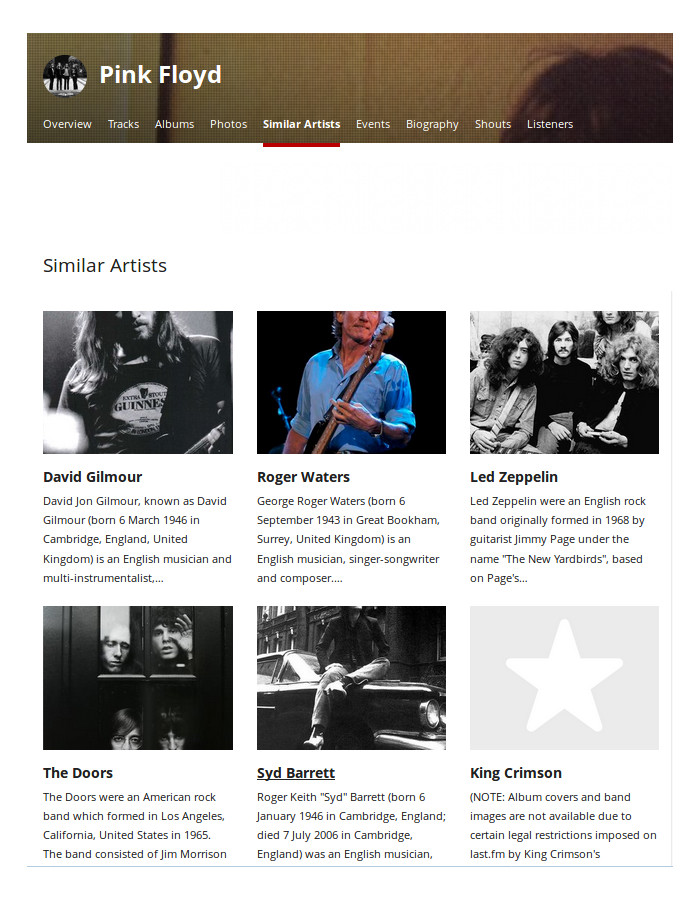
\includegraphics[width=7in,height=7in]{pics/lstfm-rs-example.jpeg}
\end{center}
\end{figure}

В момент решения задачи $topN$ и в момент проверки качества решения
в ООМ используется информация только
о тех объектах, для которых известно, что $(u_a \R i_0) \wedge (u_a \R
i_{\bot})$\footnote{
	Во-первых, данная информация является достаточной для решения задачи
	$topN$, а, во-вторых, информация о других значениях $\rho(u, i)$
	может быть недоступна. К примеру, для случая интернет-магазина, где
	существует только факт наличия приобретения товара без его оценки.
	},
поэтому при решении задачи $topN$ будем работать с множеством исходных
данных вида $P = \{(u, i, \rho(u, i)): u \R i \}$.

Правило вывода $\Pi_O$ ООМ для решения задачи $topN$ задается следующей формулой:
\begin{equation}
	\label{ors-pi-top}
	i \rt i_0 \Rightarrow (\rh(u_a, i) := 1) \wedge (u_a \R i)
\end{equation}
Значения $\rh(u_a, i)$ задаются равными единице, потому что тогда объекты $i$
будут близкими для активного пользователя при любом пороговом значении
$\Delta_{\R}$.
Правило вывода $\Pi_O$ говорит о том,
что если существует объект $i$, являющийся соседом для объекта $i_0$,
то, следуя эвристическому утверждению модели (\ref{assertORS1}), выполняется
отношение $u_a \R i$,
так как $u_a \R i_0$ по принятому для задачи $topN$ виду исходного множества.
То есть решение можно записать в форме утверждения: $(u_a \R i_0) \wedge (i \rt
i_0) \Rightarrow u_a \R i$.

Приведем схему решения задачи $topN$ при использовании правила вывода $\Pi_O$
(\ref{ors-pi-top}). Для того, чтобы составить множество объектов, между которыми и
активным пользователем выполняется отношение близости, по правилу вывода нужно найти объекты,
между которыми и объектами обучающего множества будет выполняться отношение
близости. Тогда, следуя эвристическому утверждению, между найденными объектами
и активным пользователем будет выполняться отношение близости: пусть $i \rt
i_0$, тогда, так как по виду исходного множества, принятого для задачи $topN$
выполняется $u_a \R i_0$, по эвристическому утверждению (\ref{assertORS1})
выполняется $u_a \rt i$ ---
$(u_a \R i_0) \wedge
(i \rt i_0) \Rightarrow u_a \rt i$, --- что и требуется по задаче $topN$.

Схему решения задачи $topN$ можно описать как формирование кластера
объектов $\nit = \{ i : i \rt I^a_0 \}$,
$|\nit| = N$, где
$I^a_0 = \{i_0: \rho(u_a, i_0) \in P_0\}$ --- центр кластера. Множество
объектов кластера (кроме центра) является искомым решением.

Определим способы задания отношения близости между объектом $i$ и
подмножеством объектов $I^a_0$
\label{deltaTneighbours}
 \cite{topn1,topn2,amazon-item2item,disser0}:
\begin{itemize}
	\item $I^a_0 \rt i \Leftrightarrow \Bigr( \frac{1}{|I^a_0|} \cdot \sum \limits_{i_0
		\in I^a_0} \di(i,i_0) \Bigl) \ge \Delta_i$.
		В стандартном решении  \cite{item-based} $topN$
		для определения меры близости между объектом $i$ и множеством объектов
		$I^a_0$ вычисляется сумма мер близости между объектом $i$ и объектами
		$i_0 \in I^a_0$.
		$I^a_0 \rt i \Rightarrow \Bigr( \frac{1}{|I^a_0|} \cdot \sum \limits_{I^a_0 \in I^a_0}
		\di(i,I^a_0)\Bigl) \ge \Delta_i \Rightarrow \exists$
$i_0 \in I^a_0, I^a_0 \rt i$.
По данным задачи и вследствие выполнения отношения $I^a_0 \rt i$, выполняется
		$(u_a \R I^a_0) \wedge (I^a_0 \R i) \Rightarrow u_a \R i$. Таким образом,
если объект $i$ принадлежит кластеру $\nit$ (то есть выполняется
		$I^a_0 \rt i$), то по утверждению ООМ  (\ref{assertORS1}) выполнится $u_a \R i$.
Поэтому данный способ определения отношения $i \rt I^a_0$ можно
		применять с правилом вывода $\Pi_O$ (\ref{ors-pi-top}) для решения задачи

\item $I^a_0 \rt i \Leftrightarrow$  $\exists I^a_0 \in I^a_0, I^a_0 \rt i$.
По данным задачи и способу задания $I^a_0 \rt i$ выполняется утверждение ООМ, то есть
		$(u_a \R I^a_0) \wedge (I^a_0 \rt i) \Rightarrow u_a \R i$.

Таким образом, если объект $i$ принадлежит кластеру $\nit$ (то есть $I^a_0 \rt i$),
		то по утверждению ООМ (\ref{assertORS1}) выполнится $u_a \R i$, что и требуется
от задачи.
Поэтому данный способ определения отношения $i \rt I^a_0$ можно
		применять с правилом вывода $\Pi_O$ (\ref{ors-pi-top}) для решения задачи
$topN$.
\end{itemize}
%%% Для вычисления значения меры близости между объектами системы может использоваться самая различная информация об объектах, которая
%%% зависит от реализации и предметной области РС\footnote{Поэтому при описании схемы, как 
%%% правило, не уделяется внимание контентам объектов}. К примеру, для кинематографической РС сценарий рекомендаций можно описать так: 
%%% если пользователь приобрел коллекцию DVD <<Крестный отец>>, то система может произвести рекомендации тех DVD, 
%%% где участвует Марлон Брандо, режиссером которых является Френсис Форд Коппола, или в жанре криминальная драма. 
%%% То есть характеристиками объекта может выступать любая
%%% известная и значительная информация о нем, в данном случае это: известный актер, режиссер и жанр.
%%--------------------------------------------
\bigbreak
Опишем один из вариантов исполнения ООМ и решим
задачу $topN$  \cite{item-based}.%TODO: set cite
\begin{itemize}
	\item $c_X(u_a) = (x_1, x_2, ..., x_|I|)$
		\begin{equation*}
			x_i =
			\begin{cases}
				1, &\text{если $u_a \R i$}\\
				0, &\text{иначе}
			\end{cases}
		\end{equation*}
		контент активного пользователя --- вектор {\it бинарных} оценок,
		отображающий информацию о том, какие объекты пользователь предпочитает.
		Примером такого контента является контент пользователя
		РС Amazon \cite{amazon-item2item}, где $x_i = 1$ означает то, что пользователь
		приобрел товар $i$;
	\item контент объекта в исследованиях РС, как правило,
		не определяется, так как множество характеристик объектов,
		их значений и структура контента не влияют на технику решения и могут
		варьироваться для различных реализаций РС. В описываемой модели
		воспользуемся векторным представлением, то есть
		$c_Y = (y_1,...,y_{|Y|})$;
	\item
		$\di(i,j) =\cos(\angle(c_Y(i),c_Y(j)))$.

		Типичной мерой близости, используемой при решении задачи $topN$ является
		косинус угла между контентами объектов, представляемых в виде векторов
		\cite{item-based,rs-handbook}.
	\item
		Чтобы не производить расчеты меры близости при формировании
		$\overline{P}^a_{\bot}$ каждый раз, когда активный пользователь
		делает запрос на решение задачи $topN$, значения мер близости $\di$
		рассчитываются заранее и заносятся в специальную матрицу $\mathbb{M}$
		размера $|I| \times |I|$:
		\begin{equation*}
			\mathbb{M}_{ij} =
			\begin{cases}
				\di(i,j), & i \ne j \\
				0, & \text{иначе}
			\end{cases}
		\end{equation*}

		Такой предварительный этап называется построением модели \cite{topn2}.
\end{itemize}

На рисунке (\ref{dia:matrix}) изображена блок-схема алгоритма
построения матрицы $\mathcal{M}$, которой соответствует псевдокод, представленный на изображении <<Алгоритм построения матрицы мер близости объектов>>  (\ref{alg:matrix})
\begin{figure}[htb]
	\caption{Блок-схема алгоритма построения матрицы $\mathcal{M}$}
\begin{center}
	\label{dia:matrix}
 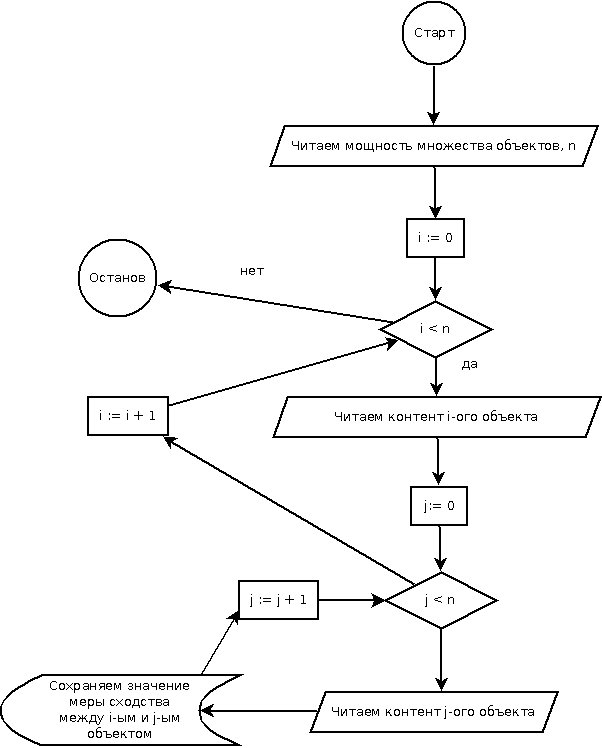
\includegraphics[width=6in,height=7in]{pics/algs/matrix.png}
\end{center}
\end{figure}

%\begin{figure}[htbp]
\begin{figure}[htb]
\caption{Алгоритм построения матрицы мер близости объектов}
\label{alg:matrix}
%\begin{algorithm}
\begin{algorithmic}[1]
\For{$i \gets 1, i \le n$}
	\State $\mathbb{M}_{ii} \gets 0$ \Comment{Чтобы пара с одинаковыми
	объектами не участвовала в дальнейших расчетах}
  \For{$j \gets 1, j \le n$}
  \State $\mathbb{M}_{ij} \gets \di(i,j)$
  \State $\mathbb{M}_{ji} \gets \mathbb{M}_{ij}$
  \State $j \gets j + 1$
  \EndFor
\State $i \gets i + 1$
\EndFor
\end{algorithmic}
%\end{algorithm}
\end{figure}

Для нахождения решения задачи $topN$ построим вектор
$\mathit{M} = (\overline{x}_1,...,\overline{x}_|I|)$, где
$
\overline{x}_i =
\begin{cases}
	0, &\text{если  $i \in I^a_0 $}\\
\mathbb{M}^i \times c_X(u_a)^T, &\text{ иначе }
\end{cases}
$\\
$c_X(u_a)^T$ --- транспонированный контент-вектор активного пользователя.
$I_{topN} = \{ i \in \{\overline{x}_i\} )\}$, где
$\{\overline{x}_i\}$ --- множество, состоящее из $N$ наибольших значений
координат вектора $\mathit{M}$.

На рисунке <<Блок-схема стандартного алгоритма решения задачи $topN$ в ООМ>> (\ref{dia:topn-solve-ors}) изображена блок-схема стандартного
алгоритма алгоритма решения задачи $topN$ в ООМ, которой соответствует
псевдокод, представленный на изображении <<Стандартный метод решения задачи $topN$ в ООМ>> (\ref{alg:topn-solve-ors})
\begin{figure}[htb]
	\caption{Блок-схема стандартного алгоритма решения задачи $topN$ в ООМ}
\begin{center}
	\label{dia:topn-solve-ors}
 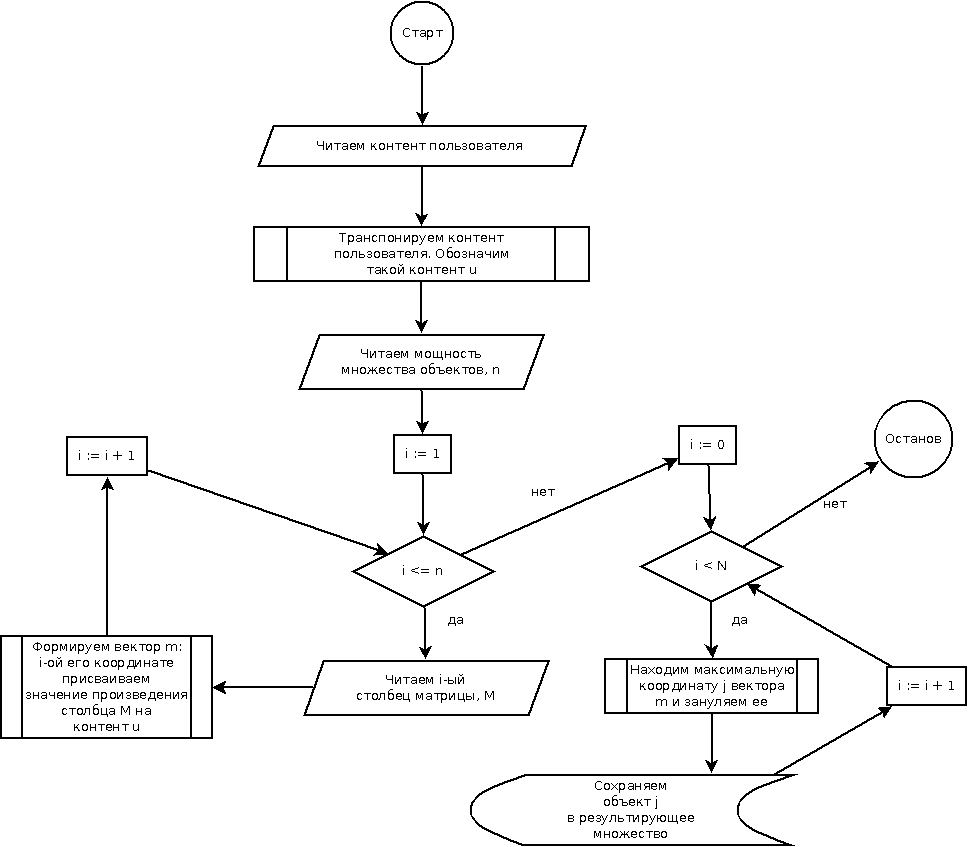
\includegraphics[width=7in,height=8in]{pics/algs/topn-ors.png}
\end{center}
\end{figure}

\begin{figure}[htb]
%\begin{algorithm}
\caption{Стандартный метод решения задачи $topN$ в ООМ}
\label{alg:topn-solve-ors}
\begin{algorithmic}[1]
\For{$i \gets 1, l \le n$} \Comment{Умножаем вектор-контент на матрицу}
	\State $m_i \gets \mathbb{M}^i \times c_X(u_a)^T$
\EndFor
\For{$j \gets 1, j \le N$}
	\State $i \gets \underset{i}{\mathrm{argmax}} \text{ } \overline{x}_i$
	\State $I_{topN} \gets I_{topN} \bigcup \{i\}$
	\Comment{Выбираем координату вектора $\mathit{M}$ с наибольшим значением}
\bigbreak
  \State $\overline{x}_i \gets 0$ \Comment{Зануляем уже выбранную координату}
  \State $j \gets j + 1$
\EndFor
\end{algorithmic}
%\end{algorithm}
\end{figure}


\subsubsection{Задача прогнозирования}
Эвристическое утверждение, на котором основывается решение задачи
$pred$ в ООМ, является более общим случаем утверждения
(\ref{assertORS1}):
\begin{assert}
	\label{assertORS2}
	Если два объекта схожи, то заданные им оценки близости пользователя будут
	приблизительно равны. \cite{rs-handbook,melville}.
\end{assert}
Данное утверждение является более общим случаем утверждения ООМ
(\ref{assertORS1}),
которое
используется при решении задачи $topN$,
так как рассматривает любые оценки, поставленные пользователем,
а не только те, которые означают, что между пользователем и объектом
выполняется отношение близости.

Во введенной терминологии данное утверждение примет следующий вид:
\begin{equation}
	i \rt j \Leftrightarrow |\rho(u,i) - \rho(u,j)|
	\le \varepsilon_p
\end{equation}

Правило вывода ООМ для решения задачи $pred$ запишется следующей
формулой:
\begin{equation}
	\label{ors-pi-p}
	\rh(u_a, i_{\bot}) = g_p(\{\rho(u_a, i^{\prime}_0)\}),
	i^{\prime}_0 \rt i_{\bot}.
\end{equation}
Правило вывода говорит о том, что оценки близости между
пользователем $u_a$ и объектами, являющимися соседями,
функционально связаны. Таким образом, зная
оценки близости, которые пользователь уже задал объектам
$i \rt i_{\bot}$, можно вычислить $\rh(u_a, i_{\bot})$
на основании функциональной связи
$g_p$.

Схема решения задачи $pred$ заключается в построении кластера
$\nip = \{ i_0 : i_0 \rt i_{\bot}\}$, центром которого является прогнозируемый
объект $i_{\bot}$. Решение задачи $pred$ запишется в виде:
\begin{equation}\label{pred-f}
	\rh(u_a,i_{\bot}) = g_p(\{\rho(u_a, i_0): i_0 \in \nip \}
\end{equation}
где $g_p$ --- некоторая функция, используемая в модели для
формирования по множеству оценок пользователя прогнозной оценки.

%===================================================================
%--------------------------------------------
%===================================================================
Опишем возможную\footnote{Модели могут отличаться такими параметрами, как,
например, функция $\di$, поэтому нижеописанная модель является одной из
возможных}
реализацию ООМ
\footnote{
	На данном этапе без оценки качества $\mathcal{E}_{topN}$
	}
 и на ее примере решим
задачу прогнозирования  \cite{item-based} %TODO: set cite. I think need
												%to see amazon
\begin{itemize}
	\item $c_X(u_a) = \{\rho(u_a,i_0)\}$
	\item $c_Y = (y_1,...,y_{|Y|})$;
	\item $\di(i,j) = \cos(\angle(c_Y(i),c_Y(j)))$
\end{itemize}
\bigbreak

Прогнозирование строится на основании оценок, поставленных активным пользователем
объектам, между которыми и прогнозируемым выполняется отношение близости.
Поиск таких объектов может осуществляться линейно по значениям, которые уже
хранятся в матрице мер близости $\mathbb{M}$, находящихся в строке с порядковым
номером, соответствующим индексу объекту. После построения кластера соседей
$\nip$,
вычисляется значение {\it прогнозной функции} от оценок пользователей,
поставленных $i \in \nip$.


На рисунке (\ref{dia:p-ors}) изображена блок-схема алгоритма
решения задачи $pred$ в ООМ.
\begin{figure}[htb]
	\caption{Блок-схема алгоритма построения матрицы $\mathcal{M}$}
\begin{center}
	\label{dia:p-ors}
 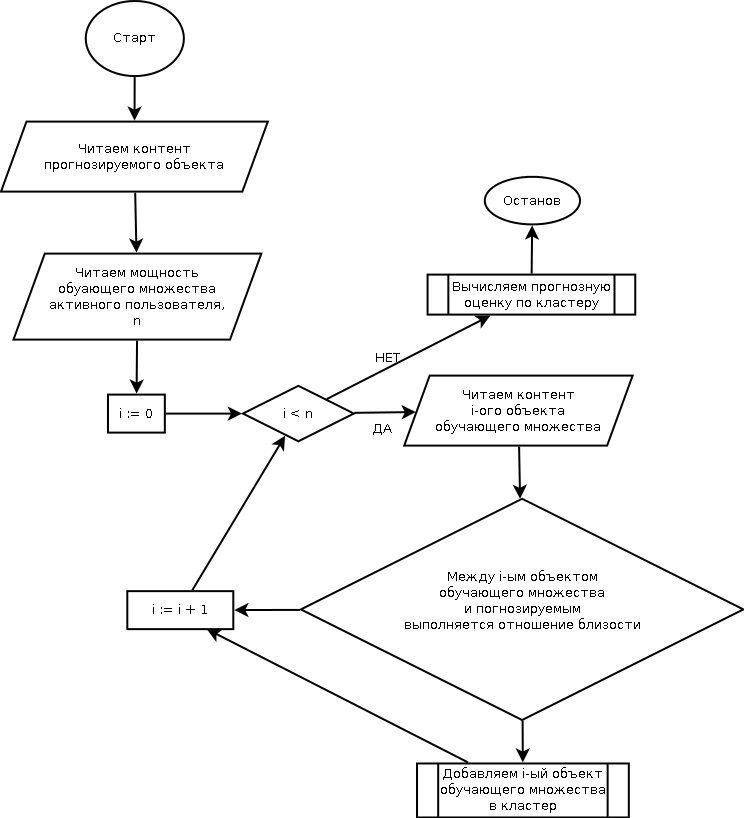
\includegraphics[width=7in,height=8in]{pics/algs/p-ors.png}
\end{center}
\end{figure}
Блок-схеме алгоритма решения задачи $pred$ в ООМ соответствует
псевдокод, представленный на изображении <<Стандартный алгоритм решения задачи $pred$ в ООМ>>  (\ref{alg:p-ors}).

\begin{figure}[htb]
\caption{Стандартный алгоритм решения задачи $pred$ в ООМ}
\label{alg:p-ors}
	%\begin{algorithm}
\begin{algorithmic}[1]
\State $\nip \gets \varnothing$\Comment{Множество объектов,
	оцененных активным пользователем и схожих с прогнозируемым объектом}
	\State $l \gets i_{\bot}$\Comment{Сохраняем в переменной $l$ индекс
	прогнозируемого объекта}
	\State $P^a \gets \varnothing$ \Comment{Множество оценок близости
	активного пользователя}
	\For {$i \in I^a_0$}
	\If {$\mathbb{M}^i_l \ge \Delta_i$}\Comment{Объект $i$ близок к
	прогнозируемому}
  \State $\nip \gets \nip \bigcup \{ i \}$
	\State $P^a \gets P^a \bigcup \{\rho(u_a,i)\}$
  \EndIf
\EndFor
\State $\rh(u_a,i) \gets g_p( P^a )$\Comment{Рассчитываем значение функции прогнозирования}
\end{algorithmic}
%\end{algorithm}
\end{figure}


\subsubsection{Функции вычисления прогнозной оценки}
Приведем
пример распространенной функции прогнозирования, применяемой в ООМ
 \cite{item-based}:
%cite
\begin{equation}\label{fpredict-ors}
	\frac{1}{|\nip|} \frac{\sum \limits_{i \in \nip} \di(i,i_{\bot}) \cdot \rho(u_a,i)}{
\sum \limits_{i \in \nip} \di(i,i_{\bot})
}
\end{equation}
%===================================================================
%--------------------------------------------
%===================================================================
\subsubsection{Используемые функции в качестве меры сходства}
\begin{itemize}
% ToDo: information retireval bib
\item \textbf{Косинус.} \newline
Наиболее популярная мера сходства, заимствованная из области
информационного поиска \cite{ir1,ir2,ir3}:
\begin{equation} \label{sim-cos}
	cos(\angle(c_Y(i),c_Y(j)) = \frac{\sum \limits_{k=1}^{|Y|} y^i_k \cdot y^j_k}{
		\sqrt{ \sum \limits_{k=1}^{|Y|} (y^i_k)^2 } \cdot
		\sqrt{ \sum \limits_{k=1}^{|Y|} (y^j_k)^2 }},
\end{equation}

\item {\bf Условная вероятность.} \newline
Данная мера сходства была разработана Кариписом \cite{topn1} для такой
предметной области РС, в которой оценки близости принадлежат бинарной
шкале. Оценки близости обладают семантикой условной вероятности
события (к примеру, приобретения товара),
которое зависит от истории поведения пользователя:
$Pr( \rho(u_a,i) = 1 | \rho(u_a,j) = 1 )$
\begin{equation}
Pr(i,j) = \frac{\tf(i \wedge j)}{\tf(i) \cdot \tf(j)^{\alpha}}
\end{equation}
где:
\begin{itemize}

\item $\tf(i)$ --- весовой коэффициент, использование которого заимствовано из
области информационного поиска, этот коэффициент определяет частоту
(от term frequency), с какой объект оценивается пользователями, то есть
$\tf(i) = |\{\rho(u,i): \rho(u,i) \in P_0\}|$,
$\tf(i ^ j) = |U^i \bigcup U^j|$,
$U^i = \{u: \rho(u_a,i) \in P_0\}$,
$U^j = \{u: \rho(u,j) \in P_0\}$.

\item $\alpha$ --- коэффициент, который служит для учета популярных объектов,
имеющих, к примеру, тенденцию быть приобретенными большинством пользователей
(и иметь, таким образом, большое значение частоты).

\end{itemize}

\item {\bf Коэффициент корреляции Пирсона.} Мера сходства,
заимствованная из статистики. Данная мера сходства использовалась
компаниями GroupLens \cite{grouplens} и Bellcore \cite{bellcore}.
\begin{equation}
 \frac{\sum \limits_{y}(y^1 - \overline{y^1}) \cdot (y^2 -
                                           \overline{y^2})}
                {\sqrt{\sum \limits_{y}(y^1 - \overline{y^1})^2 \cdot
        \sum \limits_{y}(y^2 - \overline{y^2})^2}},
\end{equation}

$\overline{y^k}$ -- среднее значение характеристики $k$-ого объекта.
\end{itemize}


\subsubsection{Примеры решения задач}
Рассмотрим примеры решения задач помощью ООМ.
\paragraph{Данные}
\begin{itemize}
\item
	Пусть контенты объектов некоторой системы представляют
		собой вектора в трехмерном пространстве характеристик $Y =
		\{y_1,y_2,y_3\}$, значения характеристик
	--- действительные числа.
	Пусть в системе существуют объекты со следующими контентами:
  \begin{enumerate}
  \item $c_Y(1) = (0,2; 0,8; 0)$;
  \item $c_Y(2) = (0; 1; 0)$;
  \item $c_Y(3) = (0,2; 1; 0)$;
  \item $c_Y(4) = (0; 0,2; 0)$;
  \item $c_Y(5) = (1; 0; 0)$;
  \item $c_Y(6) = (0,8; 0; 0)$;
  \item $c_Y(7) = (0; 0; 1)$;
  \item $c_Y(8) = (0; 0; 0,8)$;
  \item $c_Y(9) = (0; 0; 1)$;
  \end{enumerate}
\item Матрица мер сходства:\\
$\mathbb{M} = $
$
\begin{pmatrix}
0    & 0.97 & 0.99   & 0.97 & 0.24 & 0.19 & 0 & 0    & 0    \\
0.97 & 0    & 0.98   & 1    &   0  &  0   & 0 & 0    & 0    \\
0.99 & 0.98 & 0      & 0.97 & 0.58 & 0.19 & 0 & 0    & 0    \\
0.97 & 1    & 0.97   & 0    & 0.37 & 0    & 0 & 0    & 0    \\
0.24 & 0    & 0.58   & 0.37 & 0    & 1    & 0 & 0    & 0    \\
0.19 & 0    & 0.19   & 0    & 1    & 0    & 0 & 0    & 0    \\
0    & 0    & 0      & 0    & 0    & 0    & 0 & 0.98 & 1    \\
0    & 0    & 0      & 0    & 0    & 0    & 0.98 & 0 & 0.98    \\
0    & 0    & 0      & 0    & 0    & 0    & 1    & 0.98 & 0    \\
\end{pmatrix}
$
\item $c_X(u_a) = (1;1,0,0,0,0,1,0,0)$
\item $N = 2$ --- для задачи $topN$ нужно определить
	два объекта, между которыми и активным пользователем выполняется отношение
		близости;
\end{itemize}

\paragraph{Решение задачи $topN$}
\begin{enumerate}
\item В матрице $\mathcal{M}$ в каждом столбце оставляем $N$
	наибольших элементов:
$\mathcal{M'} = $
$
\begin{pmatrix}
0    & 0,97 & 0,99   & 0,97 &      & 0,19 & 0 & 0    & 0    \\
0,97 & 0    & 0,98   & 1    &   0  &  0   & 0 & 0    & 0    \\
0,99 & 0,98 & 0      &      & 0,58 & 0    & 0 & 0    & 0    \\
0    & 1    & 0      & 0    &      & 0    & 0 & 0    & 0    \\
0    & 0    & 0      & 0    & 0    & 1    & 0 & 0    & 0    \\
0    & 0    & 0      & 0    & 1    & 0    & 0 & 0    & 0    \\
0    & 0    & 0      & 0    & 0    & 0    & 0 & 0,98 & 1    \\
0    & 0    & 0      & 0    & 0    & 0    & 0,98 & 0 & 0,98    \\
0    & 0    & 0      & 0    & 0    & 0    & 1    & 0,98 & 0    \\
\end{pmatrix}
$
\item Перемножим {\it транспонированный} контент $c_X(u_a)^T$
	пользователя и матрицу $\mathcal{M'}$
		$m = (u_a)^T \times \mathcal{M'} = s = (0,97; 0,97, 1.97, 1.97, 0, 0,19, 0, 0,98, 1)$
\item Из вектора $m$ выбираем два наибольших значения. Им
	соответствуют объекты 3 и 4. Поэтому
		$I_{topN} = \{3, 4\}$.
\end{enumerate}

\paragraph{Задача прогнозирования}
Решим задачу прогнозирования для объекта 4 и активного пользователя со
следующими данными $P^a_0 = \{(2 | 1), (3, 0,1)\}$.
\begin{enumerate}
	\item $i_{\bot} = 4$ --- необходимо спрогнозировать оценку 4-ого объекта;
	\item Будем пользоваться функцией прогнозирования, описанной формулой
		(\ref{pred-f}).
	\item Составим множество соседей прогнозируемого объекта 4, для чего
		воспользуемся матрицей $\mathcal{M}$, $\nip = \{2, 3\}$
\item $\rho(u_a, 4) = \frac{1 \cdot 0.97 + 0,9 \cdot 1}{|0.97 + 1|} = 0,95$
\end{enumerate}

%===================================================================
%--------------------------------------------
%===================================================================
%===================================================================
%--------------------------------------------
%===================================================================

%-----------------------------------------------
%% \subsubsection{Примеры решения задач ООМ}
%% Рассмотрим примеры решения задач в ООМ. Будем использовать в примерах одни и те же данные
%% для каждой задачи, которые были описаны в разделе 1.3.6.

%% \paragraph{Задача top-$N$}
%% Решим задачу top-$N$ при $N=2$. Известно, что 
%% $I^a = \{ (i^1; 0,9), (i^2; 0,75), (i^5; 0,5), (i^6; 0,3), (i^{10}; 0,8)  \}$, поэтому контент активного пользователя
%% при решении задачи top-$N$ представляется в виде следующего вектора:
%% $a =
%% \begin{pmatrix} 
%% 1\\
%% 1\\
%% 0\\
%% 0\\.Ь = 
%% 0\\
%% 0\\
%% 0\\
%% 0\\
%% 0\\
%% 1\\
%% \end{pmatrix}
%% $
%% \begin{enumerate}
%% \item Предварительно проведем этап моделирование, в ходе которого построим матрицу оценок сходства $\mathbb{M}$
%% $
%% \begin{pmatrix} 
%% 0    & 0,99 & 0,76 & 0,47 & 0,62 & 0,07 & 0,98 & 0    & 0,26 & 0,7  \\
%% 0,99 &  0   & 0,74 & 0,5  & 0,69 & 0,14 & 0,96 & 0,08 & 0,35 & 0,74    \\
%% 0,76 & 0,74 & 0    & 0,8  & 0,39 & 0,31 & 0,85 & 0,21 & 0,24 & 0,1   \\
%% 0,47 & 0,5  & 0,8  & 0    & 0,63 & 0,81 & 0,55 & 0,74 & 0,69 &   0  \\
%% 0,62 & 0,69 & 0,39 & 0,63 & 0    & 0,71 & 0,54 & 0,7  & 0,91 & 0,91   \\
%% 0,07 & 0,14 & 0,31 & 0,81 & 0,71 & 0    & 0,08 & 0,99 & 0,92 & 0  \\
%% 0,98 & 0,96 & 0,85 & 0,55 & 0,54 & 0,08 & 0    &  0   & 0,21 &   0,57 \\
%% 0    & 0,08 & 0,21 & 0,74 & 0,7  & 0,99 & 0    &  0   & 0,92 &  0  \\
%% 0,26 & 0,35 & 0,24 & 0,69 & 0,91 & 0,92 & 0,21 & 0,92 & 0    & 0,37   \\
%% 0,7  & 0,74 & 0,1  & 0    & 0,91 & 0    & 0,57 &  0   & 0,37 & 0    \\
%% \end{pmatrix}
%% $

%% \item В полученной матрице в каждом столбце оставляем $N (=2)$ наибольших элементов:
%% $\mathcal{M'} = \\$
%% $
%% \begin{pmatrix} 

%% \end{pmatrix}
%% $
%% \item Перемножим {\it транспонированный} вектор-контент пользователя и матрицу, полученную в пункте 4:
%% $(u_a)^T \bot \mathcal{M'} = s = (0.97, 0.97, 1.97, 1.97, 0, 0.19, 0, 0.98, 1) \Rightarrow I^a_{topN} = \{i^3, i^4\}$
%% \end{enumerate}
%% \paragraph{Задача прогнозирования}
%% \begin{enumerate}
%% \item Из вида матрицы и условия\ref{example-cond}  следует, что что $\{i^1,i^2,i^3\}$ --- множество объектов, схожих с прогнозируемым;
%% \item $\rho(u_a, i^4) = \frac{1 \cdot 0.97 + 0.9 \cdot 1}{|0.97 + 1|} = 0.95$
%% \item Результат прогнозирования соответствует результату задачи top-$N$, так как $vp^a_l = 9.5 \Rightarrow a \R i$, и $i \in I^a_{topN}$
%% \end{enumerate}



%% \subparagraph{Характеристика объектно-ориентированных систем}
%% \subsubparagraph{Асимптотическая сложность решения и модели}
%% Для построения матрицы мер сходства необходимо вычислить $\frac{1}{2} \cdot (|T| - 1) \cdot |T|$ раз меру сходства. Сложность вычисления меры 
%% сходства зависит от мощности $C_T$. Однако $|CT| << |T|$, поэтому будем считать, что сложность вычисления меры сходства -- константа,
%% а {\bf асимптотическая сложность} определяется формулой $O(|T|^2)$.
%% {\bf  асимптотическая сложность} решения определяется умножением матрицы на вектор, она равна $O(|T|^2)$.

%% % ToDo сослаться на Сашину систему
%% Сложность данного решения велика, учитывая тот факт, что, как правило, в реальных систем $T$ огоромно. К примеру, 
%% новостная лента каждый день пополняет свою базу более, чем на 100 статей объектов. Таким образом, модель и решение
%% ООМ обладает {\it слабой масштабируемостью}.
%


%-----------------------------------------------


%%%\chapter{Субъектно-ориентированные эвристические коллаборативные системы}
\subsection{Субъектно-ориентированная модель рекомендательной
системы}
Одой из первых РС, в которой была применена
СОМ для решения задач, --- это РС, разработанная компанией
GroupLens \cite{grouplens}.

СОМ проводят анализ предпочтений
пользователей. Отфильтровываются те пользователи, чьи предпочтения не близки.
Если пользователи близки
по предпочтениям, то между ними выполняется отношение близости, и тогда
информация о таких пользователях используется для решения задачи. В
исследованиях, посвященных СОМ, такие пользователи называются
соседями \cite{neighbor-cf}.
Для РС интернет-магазина близость по предпочтениям может
выражаться, к примеру, тем, что пользователи приобретают одни и те
же товары (то есть объекты) \cite{e-commerce}.

В СОМ характеристиками пользователей являются объекты,
значениями характеристик --- значения $\rho(u, i)$, которые определяют
предпочтения пользователей.
В общем случае соседями считаются те пользователи,
кто одинаково оценивает одни и те же объекты, что во введенной
терминологии запишется в следующем виде:
\begin{equation}
	\label{user-sim1}
	u \ru v \Leftrightarrow \forall i: \exists \rho(u,i) \wedge
	\exists \rho(v,i) \text{ верно, что } |\rho(u,i) -
	\rho(v,i)| \le \varepsilon_p,
\end{equation}
где $\varepsilon_p$ --- некоторая малая фиксированная величина.

Определим отношение близости на основании меры близости
$\du: U \times U \rightarrow [0,1]$. Считается,
что если мера близости между пользователями больше некоторого порогового
значения, то пользователи являются соседями  \cite{threshold1, threshold2,
threshold3,threshold4,threshold5}:
\begin{equation}
	\label{user-sim2}
	u \ru v \Leftrightarrow \du(u,v) \ge \Delta_u, \Delta_u \in
	[0,1]
\end{equation}
Стоит отметить, что при разработке СОМ необходимо подбирать
параметры $\du$ и $\Delta_u$ так, чтобы близкие пользователи по определению
\ref{user-sim1}, были близки по определению \ref{user-sim2}:
важность подбора таким образом параметров будет описана в главах, посвященных
анализу коллаборативной фильтрации и последующих после текущей главы.

Правило вывода $\Pi_C$ в СОМ основано на утверждении, которое
гласит, что если в прошлом пользователи были близки по вкусам,
то и в будущем они будут близки по вкусам \cite{ub-assumption}.
Во введенной
терминологии данное утверждение примет следующий вид:
\begin{equation}
\label{srs-assert}
u_a \ru u \text{ выполняется на } P_0 \Rightarrow u_a
\ru u \text{ выполняется на } P_{\bot}
\end{equation}
Во время проведения тестов множеством будущего выступает тестовое множество,
множеством настоящего --- обучающее.

Правило вывода СОМ основывается
на эвристическом утверждении \cite{cfrs}, которое гласит :
\begin{assert}\label{assertSRS1}
пользователи, схожие по предпочтениям в прошлом, будут схожи и в будущем.
\end{assert}
Поэтому утверждение
во введенной терминологии запишется следующим образом:
\begin{equation*}
	\forall i_0:
	|\rho(u,i_0) - \rho(v,i_0)| \le \varepsilon_p
	\Rightarrow \forall i_{\bot} |\rho(u,i_{\bot}) - \rho(v,i_{\bot})|
	\le \varepsilon_p,
\end{equation*}

Правило вывода $\Pi_C$ в СОМ задается следующей формулой:
\begin{equation}
	\label{srs-pi}
	u \in U, (u_a \ru u) \Rightarrow |\rh(u_a, i_{\bot}) - \rho(u_a, i_{\bot})|
	\le \varepsilon_p, \rh(u_a, i_{\bot}) = f_p(\{\rho(u, i_{\bot})\}).
\end{equation}
Правило вывода СОМ говорит о том, что если пользователи $u$ являются
соседями для пользователя $u_a$, то оценки близости $\rho(u_a, i_{\bot}), \rho(u, i_{\bot})$
коррелируют, поэтому
неизвестное значение $\rho(u_a, i_{\bot})$ можно функционально определить по
значениям $\{\rho(u, i_{\bot})\}$, то есть прогнозная функция является функцией от
значений оценок близости соседей.

Данная модель используется, в основном, для решения задачи $pred$.
%Рассмотрим, как правило вывода применяется для решения задач.
%%%%%%%%%%%%%%%%%%%%%%%%%%% TOPN %%%%%%%%%%%%%%%%%%%%%%%%%%%%%%%%%%%%%%%%%%

\subsubsection{Задача $topN$}
Схема решения задачи $topN$ заключается в построении кластера соседей
$\nut = \{u: u_a \ru u\}$ активного пользователя $u_a$, который выступает в
роли центра кластера. После того, как кластер был
построен, выбирается $N$ объектов, которые близки для большинства
пользователей.

Это решение основано на правиле вывода $\Pi_C$ --- пусть объект $i$ близок
для большинства пользователей кластера $\nut$: $(\frac{1}{|\nut|} \sum \limits_{u \in
\nut} \rho(u,i)) \ge \Delta_{\R}$, а функциональная зависимость $f_p$
прогнозной функции $\rh$ определяется средним значением оценок близостей
соседей $\rho(u,i)$. Тогда $\rh(u_a, i) = f_p(\{\rho(u, i)\})
> \Delta_{\R}$, и тогда можно утверждать, что $u_a \R i$. $N$ таких объектов
составляет решение задачи $topN$.

Опишем возможную\footnote{Модели могут отличаться такими параметрами, как,
например, функция $\du$, поэтому нижеописанная модель является одной из
возможных}
модель CОМ
\footnote{
	На данном этапе без оценки качества $\mathcal{E}_{topN}$
	}
 и на ее примере решим
задачу $topN$  \cite{amazon-linden}.%TODO: set cite

\begin{itemize}
	\item $c_X(u_a) = (x_1, x_2, ..., x_n)$
\begin{equation*}
  x_i =
  \begin{cases}
	1, &\text{если $u_a \R i$}\\
	  0, &\text{иначе}
  \end{cases}
\end{equation*}
	Это распространенный способ представления контента,
	где координаты соответствуют объектам
		 \cite{topn1}.
	Данный способ представления
	информации о пользователях заимствован из информационного поиска
	 \cite{e-commerce,empirical-cf,ir4};
	\item $c_Y$ не определяется, так как с объектами в СОМ работа не проводится;
	\item $\di(u_a,u) =\cos(\angle(c_X(u_a),c_X(u)))$.
\end{itemize}

Чтобы сформировать кластер соседей, производится линейный поиск соседей
на множестве пользователей \cite{amazon-item2item}. Для построения результирующего
множества просуммируем контенты (данная операция
допустима, так как контент представляет из себя вектор) соседей,
и выберем те координаты $i$, которые обладают наибольшими значениями
и $(i, \rho(u_a,i)) \not \in P_0$.


На рисунке (\ref{dia:nut}) изображена блок-схема алгоритма
построения кластера соседей $\nut$, которой соответствует псевдокод
, представленный на изображении <<Построение множества соседей для активного
		пользователя $u_a$ при решении задачи $topN$>>
(\ref{alg:nut}).
\begin{figure}[htb]
	\caption{Блок-схема алгоритма построения кластера $\nut$}
\begin{center}
	\label{dia:nut}
 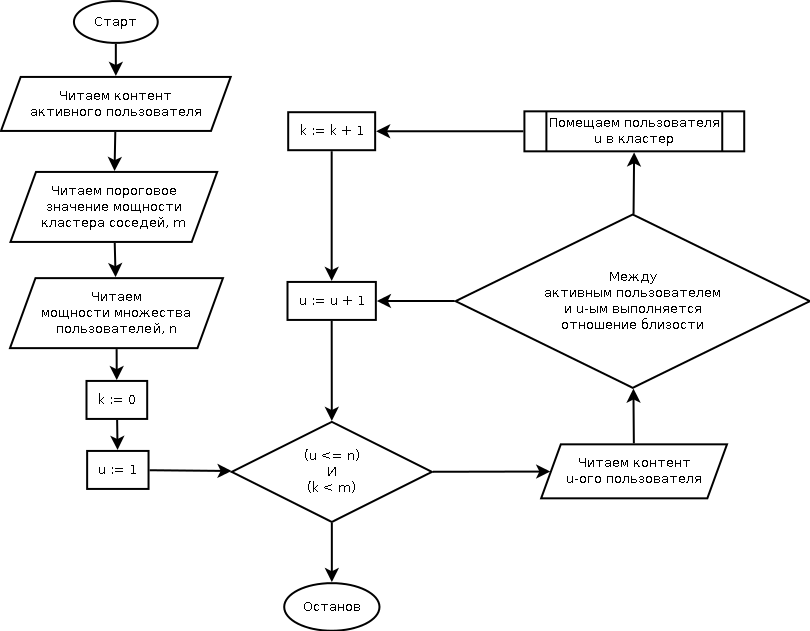
\includegraphics[width=7in,height=8in]{pics/algs/nut.png}
\end{center}
\end{figure}

\begin{figure}[htbp]
	%\begin{algorithm}
		\caption{Построение множества соседей для активного
		пользователя $u_a$ при решении задачи $topN$}
		\label{alg:nut}
		\begin{algorithmic}[1]
			\State $\nut \gets \varnothing$
			\State $k \gets 0$
			\For {$u \gets 1 \to |U|$}
			\If{$u_a \ru u$}
			\State $\nut \gets \nut \bigcup \{ u \}$
			\State $k \gets k + 1$
			\EndIf
			\If{$k > M$}\Comment{Ограничение на размер множества соседей}
			\State Стоп
			\EndIf
			\EndFor
		\end{algorithmic}
	%\end{algorithm}
\end{figure}


На рисунке (\ref{dia:topn-srs}) изображена блок-схема решения задачи $topN$ в
$COM$, которой соответствует псевдокод, представленный на изображении <<Стандартный алгоритм решения задачи $topN$>>  (\ref{alg:topn-srs}).
\begin{figure}[htb]
	\caption{Решение задачи $topN$ в $COM$}
	\begin{center}
		\label{dia:topn-srs}
		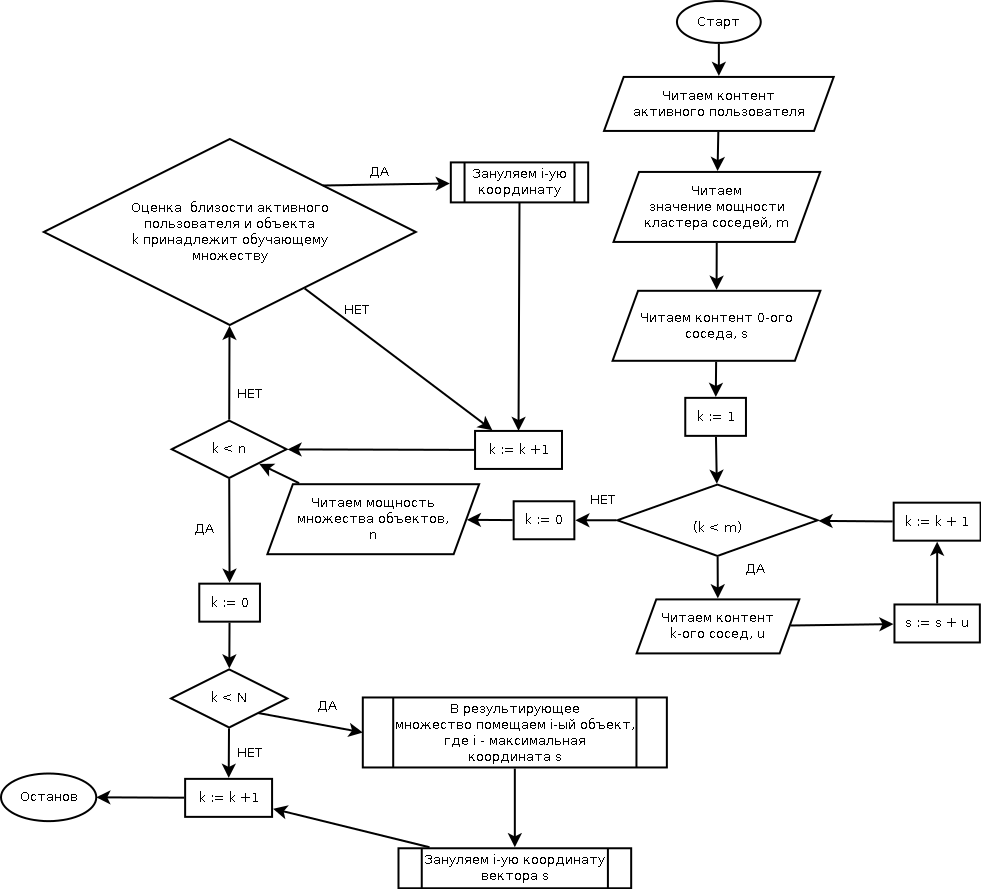
\includegraphics[width=7in,height=8in]{pics/algs/topn-srs.png}
	\end{center}
\end{figure}

\begin{figure}[htbp]
	%\begin{algorithm}
		\caption{Стандартный алгоритм решения задачи $topN$}
		\label{alg:topn-srs}
		\begin{algorithmic}[1]
			\State $s \gets \sum \limits_{u \in \nut} u$ \Comment{Вектор-сумма}
			\For {$i \gets 1, i \le |I|$}
			\If {$\exists \rho(u_a,i)$} \Comment{Если активный пользователь уже оценил
			объект, то он должен отсутствовать в результирующем множестве}
			\State $s_i \gets 0$ \Comment{Зануляем $i$-ую координату}
			\EndIf
			\EndFor
			\State $\overline{P}^a_{\bot} \gets \varnothing$
			\State $I_{topN} \gets \varnothing$
			\For {$k \gets 1, k \le N$}
			\State $i \gets \underset{i} {\mathrm{\max}}$ $s$
			\State $I_{topN} \gets I_{topN} \bigcup \{i\}$
			\State $\overline{P}^a_{\bot} \gets \overline{P}^a_{\bot} \bigcup
			\{ 0 \}$ \Comment{Для решения задачи нужно составить множество объектов, а не
			определить близость, поэтому $\rho(a,i)=0$, так как тогда $\forall
			\epsilon_0:$ $u_a \R i$}
			\State $s_i \gets 0$
			\State $k \gets k + 1$
			\EndFor
		\end{algorithmic}
	%\end{algorithm}
\end{figure}


\subsubsection{Задача прогнозирования}
Подобно задаче $topN$, для решения задачи $pred$ \cite{cfrs, cf-expert,
rs-handbook, toward,coscial-rec-survey, user-item-cf,rs-cf}
строится кластер соседей, центром которого является активный пользователь
$u_a$, однако в кластер входят не только те пользователи, между которыми
и активным выполняется отношение близости, но и такие, которые оценили
прогнозируемый объект $i_{\bot}$:
$\nup = \{u: u_a \ru u \wedge \rho(u,i_{\bot}) \in P_0\}$. Такое дополнительное
условие накладывается для того, чтобы по известным $\rho(u, i_{\bot}), u \in \nup$
определить неизвестную $\rho(u,i_{\bot})$.
Следуя утверждению СОМ (\ref{assertSRS1}), $\forall$ $u \in \nup$ выполняется $|\rho(u_a,i_{\bot}) -
\rho(u,i_{\bot})| \le
\varepsilon_p$.
Для того, чтобы рассчитать прогнозную оценку,
вычисляется значение некоторой прогнозной функции $f_p$
от оценок, поставленных прогнозируемому объекту соседями:
\begin{equation}
	\rh(u_a,i_{\bot}) = f_p(\{ \rho(u,i_{\bot}): u \in \nup \})
\end{equation}

На рисунке (\ref{dia:nup}) изображена блок-схема алгоритма
построения кластера соседей $\nup$, которой соответствует псевдокод
(\ref{alg:nup}).
\begin{figure}[htb]
	\caption{Блок-схема алгоритма построения кластера $\nup$}
\begin{center}
	\label{dia:nup}
 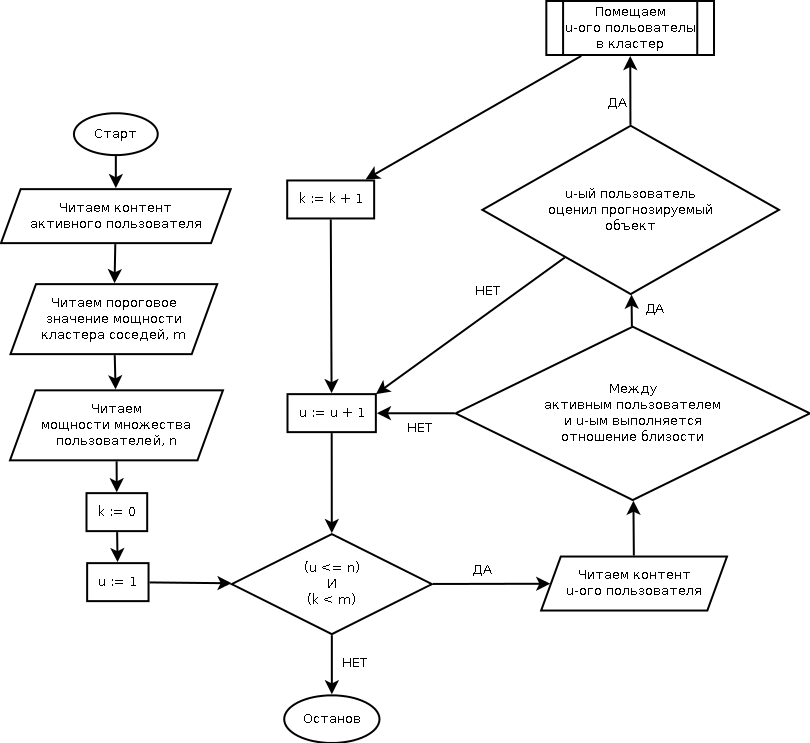
\includegraphics[width=7in,height=8in]{pics/algs/nup.png}
\end{center}
\end{figure}

\begin{figure}[htb]
	%\begin{algorithm}
		\caption{Построение множества соседей для активного
		пользователя при решении задачи прогнозирования в СОМ}
		\label{alg:nup}
		\begin{algorithmic}[1]
			\State $\nup \gets \varnothing$
			\State $k \gets 0$
			\For {$u \gets 1 \to |U|$}
			\If{($u_a \ru u$) $\wedge$ $(\exists$ $\rho(u, i_{\bot}))$}
			\State $\nup \gets \nup \bigcup \{ u \}$
			\State $k \gets k + 1$
			\EndIf
			\If{$k > M$}\Comment{Ограничение на размер множества соседей}
			\State Стоп
			\EndIf
			\EndFor
		\end{algorithmic}
	%\end{algorithm}
\end{figure}

Стандартный алгоритм решения задачи $pred$ в СОМ производится
в две итерации, которым соответствует псевдокод, представленный на изображении <<Стандартный алгоритм решения задачи прогнозирования в СОМ>>
 (\ref{alg:p-srs}):
\begin{enumerate}
	\item формирование кластера соседей $\nup$ (\ref{alg:nup});
	\item вычисление прогнозной функции по множеству оценок $\{\rho(u, i_{\bot}): u
		\in \nup\}$.
\end{enumerate}

\begin{figure}[htb]
	\caption{Стандартный алгоритм решения задачи прогнозирования в СОМ}
	\label{alg:p-srs}
		\begin{algorithmic}[1]
			\State $\nup$ \Comment{Формируем кластер соседей}
			\State $\rh(u_a, i_{\bot}) \gets f(\{\rho(u, i_{\bot}): u
			\in \nup\})$ \Comment{Вычисляем прогнозную функцию}
		\end{algorithmic}
\end{figure}


\subsubsection{Функции вычисления прогнозной оценки}
Приведем примеры распространенных функций $f_p$, которые используются для
вычисления значения прогнозной функции по значениям $\rho(u, i), u \in \nup$.
\begin{itemize}
  \item Среднее  \cite{surveyCf}:
  \begin{equation}
	\label{middle-pred}
    \frac{1}{|\nup|} \cdot \sum \limits_{u \in \nup} \rho(u,i_{\bot}).
  \end{equation}
  \item Среднее взвешенное \cite{surveyCf}:
  \begin{equation}
	  \label{weighted-pred}
    \overline{\rho^a} +
    \frac{ \sum \limits_{u \in \nup} \du(u_a,u) \cdot (\rho(u,i_{\bot}) -
	  \overline{\rho^u}) }
{ \sum \limits_{u \in \nup} | \du(u_a,u) | }
  \end{equation}
  $\overline{\rho^a}$ --- среднее значение близости активного пользователя,
		$\overline{\rho^u}$ --- среднее значение близости пользователя $u$.
Вычитание средней оценки близости призвано устранить эффект,
который накладывается от характера пользователя:
		лояльные пользователи ставят оценки близости не ниже определенной,
строгие пользователи --- наоборот \cite{norm, rs-handbook}.

Приведенные способы вычисления прогнозной оценки являются распространенными, но не единственными.
К примеру, компания Ringo \cite{ringo} не использовала в своей системе веса,
а среднее значение меры сходства соседей. Однако
метод среднего взвешенного является не только простым и распространенным,
но и согласуется с
теорией общественного выбора, ее обоснованиями человеческого поведения, ---
первичными принципами коллаборативной фильтрации  \cite{cfrs,bellcore}.
\end{itemize}

%%%%%%%%%%%%%%%%%%%%%%%%%%%%%%%%%%%%%%%%%%%%%%%%%%%%%%%%%
\subsubsection{Меры сходства}
Приведем примеры распространенных функций, которые используются в качестве меры
сходства.
\begin{itemize}
\item Коэффициент корреляции Пирсона\label{pearson}:
\begin{equation}
	\du(u,v)\frac{\sum \limits_{i \in I_{\bigcap}}(\rho(u,i) - \overline{\rho}^u) \cdot
	(\rho(v,i) - \overline{\rho}^v)}
                {\sqrt{\sum \limits_{i \in I^u}(\rho(u,i) - \overline{\rho})^u \cdot
                    \sum \limits_{i \in I^v}(\rho(v,i) - \overline{\rho}^v)^2}}
\end{equation}
\begin{equation*}
	I^a = \{i: (i, \rho(a,i)) \in P^a_0\}, a \in \{u,v\},P^a_0 = \{\rho(a, i_0)\}
\end{equation*}
\begin{equation*}
	I_{\bigcap} = I^u \bigcap I^v
\end{equation*}
\item Косинус угла между контентами.
	Для применения этой меры сходства необходимо представлять
контенты как элементы векторного пространства, в котором координата
		соответствует объекту и равна нулю, если пользователь не оценивал
		данный объект.
\begin{equation}
cos(\angle(u,v) = \frac{\sum \limits_{ i \in I_{\bigcap} } \rho(u,i) \cdot \rho(v,i)}{
\sqrt{ \sum \limits_{i \in  I^u } (\rho(u,i))^2 } \cdot \sqrt{ \sum \limits_{ i \in I^v} (\rho(u,i))^2 }},
\end{equation}
\end{itemize}


\subsubsection{Примеры решения задач}
Рассмотрим примеры решения задач в СОМ.
\paragraph{Данные}
\begin{itemize}
\item $N=2$ --- для задачи $topN$ требуется определить 2 топовых объекта;
\item $i_{\bot} = 7$ --- для задачи прогнозирования необходимо спрогнозировать оценку на объект 7;
\item $\mathcal{S} = \{0,1;0,2;0,3;0,4;0,5\}$ --- оценки принадлежат относительной шкале от 1 до 5. Если оценка равна 0; то пользователь не
ставил оценку на данный объект.
\item $|I| = 10$
\item Контенты пользователей --- вектор оценок, где $i-ая$ координата соответствует $i$-ому объекту.
  \begin{itemize}
    \item $a =   (0,5; 0,2; 0,4; 0,3; 0,5; 0,0; 0,0; 0,0; 0,0; 0,0)$
    \item $u_1 = (0,5; 0,2; 0,5; 0,0; 0,4; 0,2; 0,5; 0,0; 0,0; 0,0)$
    \item $u_2 = (0,4; 0,3; 0,5; 0,0; 0,4; 0,0; 0,0; 0,4; 0,5; 0,2)$
    \item $u_3 = (0,2; 0,5; 0,2; 0,4; 0,3; 0,0; 0,0; 0,5; 0,4; 0,0)$
    \item $u_4 = (0,0; 0,0; 0,0; 0,0; 0,0; 0,2; 0,0; 0,3; 0,5; 0,5)$
    \item $u_5 = (0,4; 0,2; 0,0; 0,0; 0,4; 0,2; 0,5; 0,5; 0,0; 0,0)$
  \end{itemize}
\item $\Delta_{\R} = 0,49$
\item В качестве меры сходства будем использовать коэффициент корреляции
	Пирсона (\ref{pearson}).
\item
  \begin{equation}
    \du(u_1,u_2) > 0.8 \Rightarrow u_1 \ru u_2
  \end{equation}
\end{itemize}
\paragraph{Задача $topN$}
\begin{enumerate}
\item Составим множество соседей мощности 2. Для этого рассчитаем меру сходства между активным пользователем и другими:
  \begin{itemize}
  \item $\du(u_a,u_1) = 0,94 \Rightarrow u_1 \in \nut$
  \item $\du(u_a,u_2) = 0,57$
  \item $\du(u_a,u_3) = -0,85$
  \item $\du(u_a,u_4) = \varnothing$
  \item $\du(u_a,u_5) = 0,81 \Rightarrow u_5 \in \nut$
  \end{itemize}
\item $s = \sum \limits_{u \in \nut} u = (0,9; 0,4; 0,5; 0,0; 0,8; 0,4; 1,0; 0,5; 0,0; 0,0)$
\item Зануляем значения координат, для которых $\rho(u_a, i) \in P_0: s =
	(0,0; 0,0; 0,0; 0,0; 0,0;0,4; 1,0; 0,5; 0,0; 0,0)$
\item $I_{topN} = \{ 7, 8 \}$
\end{enumerate}
\paragraph{Задача прогнозирования}
При решении предыдущей задачи было составлено множество соседей.
Определим прогноз по оценкам этих соседей:
\begin{equation}
f_p(u_a,7) =  0,38 + \frac{ 0,94 \cdot (0,5 - 0,38) + 0,81 \cdot (0,5 - 0,36)}{
	0,94 + 0,81 } = 0,55
\end{equation}

%%%%%%%%%%%%%%%%%%%%%%%%%%% PREDICT %%%%%%%%%%%%%%%%%%%%%%%%%%%%%%%%%%%%%%%%%%
%%%%%%%%%%%%%%%%%%%%%%%%%%% PREDICT FUNCTIONS %%%%%%%%%%%%%%%%%%%%%%%%%%%%%%%%%%%%%%%%%%

%eval-sim-metrics ToDo: раписать целевую
\section{Описание функций оценок качества решений задач} \label{def-eval}

\subsection{Оценка решения задачи прогнозирования}
Данные оценки определяют, насколько {\it аккуратно} был произведен прогноз путем
расчета погрешности между спрогнозированной оценкой близости и реальной,
принадлежащей тестовому множеству.

Приведем распространенные оценки эффективности этого класса:
\begin{itemize}
\item
  \begin{equation}
	  MAE = \frac{1}{|P^a_{\bot}|} \sum \limits_{(u_a, i_{\bot}, \rho(u_a,
	  i_{\bot})) \in P^a_{\bot}} |\rho(u_a, i_{\bot})
	  - \rh(u_a, i_{\bot})|,
  \end{equation}
		где $P^a_{\bot} = \{\rho(u_a, i_{\bot})\}$ --- тестовое множество
		активного пользователя;
\item
  \begin{equation}
	  \label{nmae}
	  NMAE = \frac{1}{|P_{\bot}|} \cdot (\rho_{\max} - \rho_{\min})
	  \sum \limits_{i \in I_{\bot}} |\du(u_a, i^m_{\bot}) - \rho(u_a, i^m_{\bot})|,
  \end{equation}
$\rho_{\max}, \rho_{\min}$ --- максимальная и минимальная оценки
шкалы соответственно.

Значения $NMAE$ труднее интерпретировать по отношению к масштабу шкалы,
но они сопоставимы для шкал любого масштаба.
\item
  \begin{equation}
	  RMSE = \sqrt{\frac{1}{|P^a_{\bot}|} \sum \limits_{(u_a, i_{\bot}, \rho(u_a, i_{\bot})) \in P^a_{\bot}}
	  (\rh(u_a, i_{\bot}) - \rho(u_a, i_{\bot}))^2}
  \end{equation}
\end{itemize}

%Решение задачи прогнозирования можно рассматривать как формирование системой
%прототипа пользователя $\overline{a}$,
%в контент которого входят спрогнозированные значения.
%Тогда цель системы заключается в том, чтобы сформировать контент пользователя
%$\overline{a}$ так, что
%$a \ru \overline{a}$, то есть $\forall i_{\bot}$ $|\rho(u_a,i_{\bot}) -
%\overline{\rho}(\overline{a},i_{\bot})| \le \epsilon_0$,
%$\overline{\rho}(u_a,i_{\bot})$ --- спрогнозированная оценка.
%Но тогда и оценки эффективности будут иметь значение меньше либо равное
%$\epsilon_0$. Поэтому будем говорить, что решение эффективно, если
%значение оценки эффективности меньше либо равно $\epsilon_0$.

\subsection{Оценка решения задачи $topN$}
% ToDo добавить еще P@ и всякие NDCG
Делая запрос на решение задачи $topN$, активный пользователь $u_a$
ставит перед системой цель
определить множество $I_{topN}$ таких объектов $i$, что $u_a \R i$. Для того,
чтобы определить, насколько точно по отношению к цели было составлено множество
$I_{topN}$ применяются функции, именуемые оценками точности. Эти функции можно
описать как функции, которые сравнивают результирующее
множество с тестовым и определяют качество как точность \lq попадания \rq
объекта из результирующего множества в тестовое.
Эти функции заимствованы из области информационного поиска \cite{ir1,ir2,ir3}.
При оценке задачи $topN$ состоит из объектов, между которыми и активным
пользователем выполняется отношение близости, как и при решении задачи:
$P^a_{\bot} = \{ (u_a,  i_{\bot}, \rho(u_a, i_{\bot})): u_a \R i_{\bot}\}$.

Для определения используемых оценок точности введем функцию,
которая определяет, выполняется ли отношение $u_a \R i$:
$
s(i) =
\begin{cases}
1, &\text{$\exists$ $i_{\bot} \in I_{\bot}$: $u_a \R i_{\bot}$}\\
0, &\text{иначе}.
\end{cases}
$\\

Функция $s$, заданная таким образом соответствует цели пользователя, поэтому
оценки точности, которые определены на базе такой функции $s$ будем называть
{\it целевыми}.

Приведем пример целевых оценок точности:
\begin{itemize}
\item Точность:
	\begin{equation}
		\label{precision}
	1 - \frac{1}{N} \cdot \sum \limits_{i \in I_{\bot}} s(i);
	\end{equation}
%\item Полнота: $1 - \frac{1}{M} \cdot \sum \limits_{i \in I_{\bot}} s(i)$,
%где $M = \{|i \in \mathbb{N}^n : a \R i |\}$ ---
%число всех объектов множества $I$, для которых выполняется отношение
%близости с активным пользователем. Как правило, полнота оценивается на
%объединении результирующих множеств, полученных на большом числе тестов
%или при $N \approx M$. Будем считать, что для полноты $M = N$\label{recall-meqn};
\item Точность $P@L$ для списка объектов длины $L$:
\begin{equation}
1 - \frac{1}{L} \cdot \sum \limits_{i \in I_L} s(n),I_L \subset I_{\bot},
|I_L| = L.
\end{equation}
\item
	\begin{equation}
	AveP = \frac{1}{\sum \limits_{n=1}^{N} s(n)} \cdot
\sum \limits_{L=1}^{N},
\end{equation}
		где $P@L$ --- среднее значение $P@L$ для $L=1..N$.
	\item
		\begin{equation}
		NDCG = 1 - \frac{DCG}{IDCG},
		\end{equation}
			где $DCG = s(1) + \sum \limits_{k=1}^N
\frac{s(i_k)}{log_2(i_k)}$ --- сумма <<весов накопления>>,
где <<вес накопления>> зависит от порядкового номера
в ранжированном результирующем множестве.
Чем меньше порядковый номер объекта,
между которым и активным пользователем выполняется отношение
близости, тем результат качественней, а вес объекта больше.
		Данная оценка используется, к примеру, для поисковых систем\cite{},
		где для пользователя важно, чтобы интересующий его объект находился в
		начале результирующего списка.
\end{itemize}

Однако, совместно с ООМ эти оценки не могут использоваться, так как ООМ
не определяют функцию $\rho: U \times I$. Вместо нее используются значения
прогнозной функции, которые рассчитываются на основании правил вывода ООМ.
Подобно решению, оценка решения задачи $topN$ при применении ООМ,
основана на эвристическом утверждении (\ref{assertORS1}). Чтобы определить,
является ли объект $i \in I_{topN}$ целевым по отношению к поставленной задачи,
нужно выяснить, существует ли объект обучающего множества, являющийся соседом
для объекта $i$. Так как для объектов обучающего множества верно, что $u_a \R
i_0$, то по эвристическому утверждению (\ref{assertORS1}) получим, что $u_a \R
i$, так как $i \rt i_0$.

Для определения качества решения в ООМ используются те же целевые функции,
но их значения зависят не от функции $s$, а от функции $\overline{s}$:
$
\overline{s}(i) =
\begin{cases}
	1, &\text{$\exists$ $i_{\bot} \in I_{\bot}$: $i \rt i_{\bot}$}\\
0, &\text{иначе}.
\end{cases}
$\\
Такие оценки точности будет называть {\it объектно-ориентированными}.

           % Глава 1
\chapter{АНАЛИЗ КОЛЛАБОРАТИВНОЙ МОДЕЛИ РЕКОМЕНДАТЕЛЬНОЙ СИСТЕМЫ} \label{chapt2}


В данном разделе проведем анализ эффективности АКМ
по критериям качества решения, вычислительной
сложности и
стабильности. В том числе проведем анализ используемых оценок качества, их
объективность и применимость.

%\subsection{Отсутствие общей терминологии}
%Следует отметить, что в ряде исследований описанная в предыдущем
%разделе техника решения ООМ, основанная на
%поиске соседей,
%называется
%% Можно посмотреть статью лидена и дернуть оттуда библиографию
%item-based или item-to-item рекомендации \cite{item-based,
%amazon-item2item,heur2,topn1,topn2,item-based-cross-sell,amazon-linden}.
%Но существуют и другие названия этой техники: в некоторых
%исследованиях ее именуют
%более общим термином ---
%модельной техникой решения
%(model-based)
%\cite{topn1,empirical-cf,ringo,learning4,item-based-cross-sell,model-based1},
%так как оно является классом модельных техник
% \cite{topn2}.
%В качестве примера приведем цитаты из статей
%известных авторов. Из статьи
%\lq Item-Based $topN$ Recommendation Algorithms \rq Дж. Кариписа \cite{topn2}:
%\begin{quote}
%The focus of this article is on a particular class of model-based $topN$
%	recommendation algorithms that build the recommendation model by analyzing the
%similarities between the various items and then use these similar items to
%identify the set of items to be recommended.
%\end{quote}
%Из
%<<Fab: Content-based, collaborative recommendation>>.
%Балабанови \cite{content10}
%\begin{quote}
%In content-based recommendation one tries to recommend items similar
%to those a given user has liked in the past.
%\end{quote}
%
%Такое разнообразие названий свидетельствует о том, что в области РС не
%существует пока общей терминологии.
%
%Коллаборативная техника решения называется контентной техникой,
%так как производится анализ контента
%объекта. Возможно, разделение в названиях произошло
%от того, что коллаборативная фильтрация работает
%только с исходными данными $P$ и не анализирует
%информацию об объектах, которая хранится в контенте. Однако, как видно
%из описаний, обе техники основаны на одном и том же принципе ---
%расчете меры сходства объектов и определении соседей. Таким образом,
%техники идентичны, но имеют разные названия.

\section{Обобщение оценок качества}
Анализ качества решений будет
производится по отношению к определенным выше оценкам качества
решений (\ref{def-eval}).
Было показано, что существует два класса оценок, каждому из которых
принадлежит некоторое число функций. Прежде, чем приступить к рассмотрению
качества решений, проведем обобщение функций,
принадлежащих каждому классу,
и будем работать далее с обобщенной функцией класса, что возможно
сделать в силу того, что оценки, которые принадлежать одному классу коррелируют
между собой \cite{herloker-eval}.

%\subsection{Истинность правил вывода}
%Рассмотрим правила вывода и эвристические утверждения, на которых они основаны.
%Выполнение приведенных в первой главе эвристических
%утверждений (\ref{}) () () в существующих исследованиях не рассматриваются,
%правила вывода, основанные на них носят аксиоматический характер.
%\subsection{Условия эффективности решений}
%Прежде, чем приступить к дальнейшему описанию, обобщим оценки
%решения и в дальнейшем для изложения материала будем работать с обобщенной
%оценкой. Возможно провести обобщение и использовать одну функцию
%при описании свойств нескольких, так как оценки, которые принадлежат одному
%классу, коррелируют друг с другом.
% \cite{herloker-eval}.

\subsubsection{Обобщенная оценка качества решения задачи прогнозирования}
По задаче $pred$ необходимо вычислить такое значение
$\rh(u_a, i_{\bot})$, что $|\rh(u_a, i_{\bot}) - \rho(u_a, i_{\bot})| \le
\varepsilon_p$.
Оценки качества решения задачи $pred$
определяют погрешность
составления прогноза, то есть все функции данного класса зависят от одного и того же параметра: от
разницы между спрогнозированной оценкой близости и настоящей.
Чем меньше разница, тем значение оценки меньше и тем аккуратность выше. Функции, принадлежащие этому
классу коррелируют между собой  \cite{herloker-eval}. Поэтому можем ввести
обобщенную функцию и работать в дальнейшем с ней.
Введем и обозначим следующую обобщенную оценку
для этого класса: $\eap = NMAE$.

\begin{assert}
	\label{objectivity-eap}
	Оценка $\eap$ соответствует задаче $pred$, а потому ее значения
	являются объективным показателем аккуратности решения.
\end{assert}
Данное утверждение следует из постановки задачи и способу определения
аккуратности.
\subsection{Обобщенная оценка качества решения задачи $topN$}
Значения приведенных в предыдущем разделе оценок качества задачи $topN$ зависит
от числа
$K = |I'| = |\{i: (i \in I_{topN}) \wedge (s'(i) = 1)\}|$,
где $s' = \{s, \overline{s}\}$.

\begin{trm}
	Решение задачи $topN$ эффективно по оценке качества, если $K \ge N \cdot (1 - \varepsilon_{topN})$
\end{trm}

Покажем, что теорема верна для каждой оценки, приведенной выше \ref{def-eval}
на примере точности (а оценки качества одного класса коррелируют между собой).
%\begin{itemize}
%\item
%	Точность:
		$\eit \le 1 - \frac{K}{N} \le 1 - (1 - \varepsilon_{topN}) \le
		\varepsilon_{topN}$.
%\item Полнота: так как рассматривается при $N = M$\ref{recall-meqn},
%	то доказательство сводится к доказательству, относящемуся к  точности.
%\item Точность $P@L$ --- верно, так как данная оценка является частным случаем
%	точности. Точность может рассматриваться как $P@N$.
%Если теорема верна для $P@N$, то она верна и для $P@L$, так как $L \le N$.
%\item $AveP$: так как отношение близости выполняется для $i_k, k=1..K$,
%то $P@L = 0, l=1..K$ и
%$\eat = \frac{1}{K} \cdot \sum \limits_{L=K}^{N} P@L$.
%В худшем случае, когда $P@L=1, l=(K+1)..N$ получим, что:\\
%$\eat = \frac{N-K}{K} = \frac{N}{K} - 1 \le \frac{N}{N \cdot (1 - \varepsilon_{topN})}
%		- 1 = \frac{1}{1 - \varepsilon_{topN}} - 1$.
%В пределе при $\varepsilon_{topN} \rightarrow 0$ ($K \rightarrow N$)
%		решение эффективно для любых значений $\varepsilon_{topN} \in \varepsilon(0)$.
%
%\item $IDCG = 1 + \sum \limits_{k=2}^N \frac{1}{log_2(k)}$. Так как $s(i_k)=1,
%	k=1..K$, то $DCG=1 + \sum \limits_{n=2}^K \frac{1}{log_2(n)}$.
%$NDCG = 1 - \frac{1 + \sum \limits_{k=2}^K \frac{1}{log_2(n)}}{1 + \sum
%		\limits_{k=2}^N \frac{1}{log_2(k)}}$.
%В пределе при $K \rightarrow N$ получим, что $NDCG \rightarrow 0$, то есть решение эффективно.
%\end{itemize}

Таким образом, мы показали, что приведенные оценки зависят от величины $K$.
Тогда будем рассматривать обобщенную целевую оценку качества решения задачи
$topN$ как функцию $\eat(K)$ при применении функции $s$,
и обобщенную объектно-ориентированную оценку $\eit(K)$ при применении
$\overline{s}$.



\section{Эффективность по критерию качества решения}
Рассмотрим, какие условия влияют на эффективность решения задачи $topN$
по критерию качества. При данном рассмотрении будем анализировать значения
$\eit$, так как именно
объектно-ориентированные (а не целевые) оценки качества применяются при
тестировании ООМ.
%%%%%%%%%%%%%%%%%%%%%%%%%%%%%%%%%%%%%%%%%%%%%%%%%%%%%%%%%%%%%%%%
%%%%%%%%%%%%%%%%%%%%%%%%%%%%%%%%%%%%%%%%%%%%%%%%%%%%%%%%%%%%%%%%
%%%% SPLIP: условия
%%%%%%%%%%%%%%%%%%%%%%%%%%%%%%%%%%%%%%%%%%%%%%%%%%%%%%%%%%%%%%%%
%%%%%%%%%%%%%%%%%%%%%%%%%%%%%%%%%%%%%%%%%%%%%%%%%%%%%%%%%%%%%%%%
\subsection{Необходимые и достаточные условия эффективности решения
по критерию качества при применении правил вывода ООМ}
\subsubsection{Необходимое условие эффективности решения задачи $topN$ по
критерию качества}
\begin{trm}\label{transAssert1}
Необходимым условием эффективности решения задачи $topN$ по критерию качества
является выполнение
транзитивности отношения близости объектов на множестве
	$I^{\prime}_{topN} \bigcup I^a_0 \bigcup I^a_{\bot}$, где
	$I^{\prime}_{topN} \subset I_{topN}, |I^{\prime}| = K \ge N \cdot (1 -
	\varepsilon_{topN})$:
\begin{equation}
	(i_0 \rt i) \wedge (i_0 \rt i_{\bot})
	\Rightarrow (i \rt i_{\bot}),
	i \in I^{\prime}_{topN}
\end{equation}
\end{trm}
Покажем, что $(\eit \le \varepsilon_{topN}) \Rightarrow
\Big((i_0 \rt i) \wedge (i_0 \rt i_{\bot}) \Rightarrow i \rt i_{\bot}\Big),
i \in I^{\prime}_{topN}$.

Пусть $(\eit \le \varepsilon_{topN})$ верно. Рассмотрим выражение
$\Big((i_0 \rt i) \wedge (i_0 \rt i_{\bot}) \Rightarrow i \rt i_{\bot}\Big)$,
а, точнее, его левую часть
$(i_0 \rt i) \wedge (i_0 \rt i_{\bot})$.
По способу задания отношения близости между объектом, входящим в результирующее
множество, и центром $I^a_0$ кластера $\nit$, выполняется, что
$\forall$ $i \in I_{topN}$ $\exists$ $i_0
\in I^a_0: i_0 \rt i$. Поэтому по построению решения верно,
что $i_0 \rt i$ для всех $i$, $i_0 \in I^a_0$.
По утверждению ООМ (\ref{assertORS1}) выполняется $i_0 \rt i_{\bot}$.
Таким образом, левая часть решения выполняется по построению решения и
аксиоматике ООМ. Рассмотрим выполнение правой части выражения --- $i \rt
i_{\bot}$.

Так как решение эффективно по критерию качества (то есть $\eit \le \varepsilon_{topN}$), то $\exists$ $I^{\prime}_{topN} \subset I_{topN}$,
$I^{\prime}_{topN} = \{ i: \exists$ $i_{\bot}, i \rt i_{\bot} \}$,
$|I^{\prime}_{topN}| = K \ge N \cdot (1 - \varepsilon_{topN})$. То есть выполняется
правая часть выражения.

Таким образом, получаем, что если решение эффективно по критерию качества, то выполняется
транзитивность отношения близости для $i \in I^{\prime}_{topN}$.
Чем меньше число $K$, тем меньше раз выполняется транзитивность
отношения близости и тем решение хуже.

\subsubsection{Достаточное условие эффективности решения задачи $topN$ по
критерию качества}
\begin{trm} \label{ass:suf-topnsolve-ors}
Достаточным условием эффективности решения задачи $topN$ по критерию качества является
выполнение транзитивности отношения близости объектов на множестве
	$I^{\prime}_{topN} \bigcup I^a_0 \bigcup I^a_{\bot}$, где
	$I^{\prime}_{topN} \subset I_{topN}, |I^{\prime}| = K \ge N \cdot (1 -
	\varepsilon_{topN})$:
$\Big((i_0 \rt i) \wedge (i \rt i_{\bot})
\Rightarrow i \rt i_{\bot} \Big) \Rightarrow (\eit \le \varepsilon_{topN})$
\end{trm}

Рассмотрим выполнение левой части выражения
$(i_0 \rt i) \wedge (i \rt i_{\bot}) \Rightarrow i \rt i_{\bot}$.
По построению решения выполняется отношение $i \rt I^a_0$.
По способу задания отношения $i \rt I^a_0$ получаем, что
$\exists$ $i_0:$ $i_0 \rt i$. По утверждению ООМ (\ref{assertORS1})
выполняется $i_0 \rt i_{\bot}$. Так как выполняется транзитивность
отношения $\rt$, то получаем, что $\forall$ $i$
$\exists$ $i_{\bot} \rt i$ и выражение $(i_0 \rt i) \wedge (i \rt i_{\bot})
\Rightarrow i \rt i_{\bot}$ истинно. Поэтому $\overline{s}(i_k) = 0$
для $k=1..K$, из чего следует, что $\eit \le \varepsilon_{topN}$.

%TODO: show examples where no transitivity and solution is bad
%TODO: example with solution and properties of users preferences

%\subsubsection{Достаточное условие эффективности решения задачи прогнозирования
%по критерию качества}
%\begin{trm}
%  Достаточным условием эффективности решения по критерию качества
%	является выполнение транзитивности отношения близости объектов
%	на множестве $\nit$:
%\begin{equation}\label{suff-cond-pred-ors}
%	(i_{\bot} \rt i) \wedge (i_{\bot} \rt j)  \Rightarrow i \rt j, i,j \in
%	\nip,
%\end{equation}
%	при выполнении которого гарантируется качество
%	решения не хуже, чем $2 \cdot \varepsilon_p$.
%\end{trm}
%
%Покажем, что $((i_{\bot} \rt i) \wedge (i_{\bot} \rt j) \Rightarrow (i \rt j))
%\Rightarrow (\eap \le \varepsilon_{p})$.
%
%Оценим значение оценку эффективности для одного активного пользователя:
%$\eap = $
%$\Bigg|$ $\rho(u_a, i_{\bot}) -
%\Big( \frac{1}{\nit} \frac{\sum \limits_{i \in \nit} \di(i_{\bot}, i) \cdot
%\rho(u_a, i)}{\sum \limits_{i \in \nit} \di(i_{\bot}, i)} \Big)$ $\Bigg|$,
%где второй член разности --- это значение прогнозной функции. \\
%
%Так как в кластер $\nit$ входят такие объекты $i$, что $i \rt i_{\bot}$, то
%есть $\di(i, i_{\bot}) \ge \Delta_i$. Поэтому
%$\eap <$
%$\Bigg|$ $\rho(u_a, i_{\bot}) -
%\Big( \frac{1}{\nit} \frac{\sum \limits_{i \in \nit} \di(i_{\bot}, i) \cdot
%\rho(u_a, i)}{|\nit| \cdot \Delta_i} \Big)$ $\Bigg| <$\\
%
%$\Bigg|$ $\rho(u_a, i_{\bot}) -
%\Big( \frac{1}{\nit} \frac{\sum \limits_{i \in \nit} \Delta_i \cdot
%\rho(u_a, i)}{|\nit| \cdot \Delta_i} \Big)$ $\Bigg|=$\\
%
%$\Bigg|\frac{1}{\nit} \frac{|\nit| \cdot \Delta_i \cdot (
%\sum \limits_{i \in \nit} \Big(\rho(u_a, i_{\bot}) - \rho(u_a, i))\Big)}
%{|\nit| \cdot \Delta_i}\Bigg|=$\\
%$\frac{\Bigg|  \sum \limits_{i \in \nit} (\rho(u_a, i_{\bot}) - \rho(u_a, i)))
%\Bigg|}{|\nit|} = A$
%
%Так как выполняется свойство транзитивности, что $\forall$ $i, j \in \nit$
%верно, что $i \rt j$. Следуя утверждению ООМ (\ref{assertORS2}), получим, что
%$|\rho(u_a,i) - \rho(u_a,j)| \le \varepsilon_p$, то есть $\rho(u_a, i) \le
%\rho(u_a, j) + \epsilon_p$. Поэтому выражение
%$A \le \Bigg| \frac{1}{|\nit|} \Big(\sum
%\limits_{i \in \nit} (\rho(u_a, i) + \varepsilon_p - \rho(u_a, i_{\bot}))\Big)
%\Bigg|$. По построению кластера $\nit$ выполняется, что $i_{\bot} \rt i$,
%поэтому $|\rho(u_a, i_{\bot}) - \rho(u_a, i)| \le \varepsilon_p$.
%Поэтому $A \le 2 \cdot \varepsilon_p$.
%
%Если свойство транзитивности выполняется, то можно гарантировать, что
%задача прогнозирования в ООМ будет решена с эффективностью не хуже, чем
%$2 \cdot \varepsilon_p$. Если свойство транзитивности не выполняется, то никаких
%гарантий получения решения, близкого к эффективному не существует.
%%%%%%%%%%%%%%%%%%%%%%%%%%%%%%%%%%%%%%%%%%%%%%%%%%%%%%%%%%%%%%%%%%%%%%%
\subsection{Необходимые и достаточные условия эффективности решения
по критерию качества при применении правил вывода СОМ}

\subsubsection{Необходимое условие эффективности решения задачи прогнозирования}
Назовем множество входных данных $P^a_0 \bigcup P^a_{\bot}$
{\it репрезентативным}, если $\underset{n \rightarrow \infty} {\mathrm{\lim}}$
$|\overline{\rho}^a - \rho(u_a,i)| = 0, i=1..n$, где $P^a_0 = \{\rho(u_a,
i_0)\}$, $P^a_{\bot} = \{\rho(u_a, i_{\bot})\}$.

\begin{trm}
\label{nec-cond-pred-srs}
  Необходимым условием эффективности решения по критерию качества является выполнение
	транзитивности отношения близости пользователей на множестве $\nup$:
\begin{equation}	(u_a \ru u) \wedge (u_a \ru v) \Rightarrow (u \ru v), \forall u,v \in \nup
\end{equation}
\end{trm}

Рассмотрим доказательство при применении взвешенной средней близости
в качестве прогнозной функции \ref{weighted-pred}.
Покажем, что $(\eap \le \varepsilon_p) \Rightarrow (u_a \ru u \wedge a
\ru u  \Rightarrow u \ru v, \forall u,v \in \nup)$

Рассмотрим доказательство для $\nup = \{u,v\}$.

Оценим значение оценки эффективности по критерию:\\
$\eap = $ $\Bigg|$ $\rho(u_a, i_{\bot}) - \overline{\rho}^a +
\frac{1}{\du(u_a,u) + \du(u_a,v)} \cdot \\
\Big(\du(u_a,u) \cdot |\rho(u,i_{\bot}) - \overline{\rho}^u| +
 \du(u_a,v) \cdot |\rho(v,i_{\bot}) - \overline{\rho}^v| \Big)$
 $\Bigg|$.

Учитывая репрезентативность, получаем, что
$\rho(u_a, i_{\bot}) - \overline{\rho}^a = 0$, поэтому\\
$\eap \le \varepsilon_p + \frac{1}{\du(u_a,u) + \du(u_a,v)} \cdot
\Big(\du(u_a,u) \cdot |\rho(u,i_{\bot}) - \overline{\rho}^u| +
 \du(u_a,v) \cdot |\rho(v,i_{\bot}) - \overline{\rho}^v|\Big)$.

Так как $\Delta_u \in [0,1]$, то $\du(u_a, m) \le 1$, где $m \in \nup$ поэтому\\
$\eap = \frac{1}{\du(u_a,u) + \du(u_a,v)} \cdot
\Big(|\rho(u,i_{\bot}) - \overline{\rho}^u| + |\rho(v,i_{\bot}) - \overline{\rho}^v|\Big)$.

Так как $u_a \ru u$ $\wedge$ $u_a \ru v$, то $\du(u_a, m) > \Delta_u$, поэтому

$\eap \le \frac{1}{2 \cdot \Delta_u} \cdot \Big(|\rho(u,i_{\bot}) - \overline{\rho}^u| + |\rho(v,i_{\bot}) - \overline{\rho}^v|\Big)$.

Оценим сумму модулей в скобках:
\begin{enumerate}
	\item Пусть $(\rho(u,i_{\bot}) \ge  \overline{\rho}^u)$ $\wedge$
		$(\rho(v,i_{\bot}) \ge  \overline{\rho}^v)$. Тогда: \\
		$(\rho(u,i_{\bot}) - \overline{\rho}^v) + (\rho(v,i_{\bot}) -
		\overline{\rho}^u)$.
		Учитывая репрезентативность перепишем
		сумму в виде: $(\rho(u,i_{\bot}) - \rho(v,i_{\bot}) + \varepsilon_p) +
		(\rho(v,i_{\bot}) - \rho(u,i_{\bot}) + \varepsilon_p)$ = $2 \cdot
		\varepsilon_p$.
		Так как решение
		эффективно, то получим $\frac{2 \cdot \varepsilon_p}{2 \cdot \Delta_u} \le \varepsilon_p$.
		Выполнение
		неравенства возможно при выполнении следующего условия:
		$\Delta_u = 1$. Если $\Delta_u = 1$, то выполнение отношения $u \ru v$
		возможно при $\du(u, v) = 1$, и используемые функции в качестве
		мер сходства (косинус, коэффициенты корреляции и т.д.) будут обладать
		свойством транзитивности. Поэтому
		$(u_a \ru u )\wedge (u_a \ru v)  \Rightarrow u \ru v, m \in \nup$,
		где левая часть выражения верна в силу построения решения.

\item $\rho(u,i_{\bot}) \le  \overline{\rho}^u$ $\wedge$ $\rho(v,i_{\bot}) \le  \overline{\rho}^v$: \\
$(\overline{\rho}^v - \rho(u,i_{\bot})) + (\overline{\rho}^u - \rho(v,i_{\bot}))$. В силу репрезентативности перепишем
сумму в виде: $(\rho(u,i_{\bot}) - \rho(v,i_{\bot})) + (\rho(v,i_{\bot}) - \rho(u,i_{\bot}))$. Дальнейшее доказательство приведено в пункте 1.

\item $\rho(u,i_{\bot}) \ge  \overline{\rho}^u$ $\wedge$ $\rho(v,i_{\bot}) \le  \overline{\rho}^v$: \\
$(\rho(u,i_{\bot}) - \overline{\rho}^v) + (\overline{\rho}^u - \rho(v,i_{\bot}))$. В силу репрезентативности перепишем
сумму в виде: $(\rho(u,i_{\bot}) - \rho(v,i_{\bot})) + (\rho(u,i_{\bot}) - \rho(v,i_{\bot}))$. Дальнейшее доказательство приведено в пункте 1.

\item $\rho(u,i_{\bot}) \le  \overline{\rho}^u$ $\wedge$ $\rho(v,i_{\bot}) \ge  \overline{\rho}^v$: \\
$(\rho(u,i_{\bot}) - \rho(v,i_{\bot})) + (\rho(v,i_{\bot}) - \rho(u,i_{\bot}))$. Дальнейшее доказательство приведено в пункте 1.
\end{enumerate}

\subsubsection{Достаточное условие эффективности решения задачи прогнозирования
по критерию качества}
\begin{trm}
\label{suf-cond-pred-srs}
Достаточным условием эффективности решения по критерию качества является выполнение транзитивности
отношения близости пользователей на множестве $\nup$:

\begin{equation}
	\Big((u_a \ru u) \wedge (u_a
	\ru v)  \Rightarrow u \ru v, m \in \nup)\Big) \Rightarrow (\eap \le \varepsilon_p)
\end{equation}
\end{trm}

Аналогично предыдущему разделу оценим значение оценки эффективности для $\nup = \{u,v\}$:

$\eap < \frac{1}{2 \cdot \Delta_u} \cdot \Big(|\rho(u,i_{\bot}) - \overline{\rho}^u| + |\rho(v,i_{\bot}) - \overline{\rho}^v|\Big)$.

Оценим сумму модулей в скобках: $|\rho(u,i_{\bot}) - \overline{\rho}^u| + |\rho(v,i_{\bot}) - \overline{\rho}^v|$.
\begin{enumerate}
	\item Пусть $(\rho(u,i_{\bot}) \ge \overline{\rho}^u)$ $\wedge$
		$(\rho(v,i_{\bot}) \ge \overline{\rho}^v|)$, тогда:\\
 $(\rho(u,i_{\bot}) - \overline{\rho}^v) +
(\rho(v,i_{\bot}) - \overline{\rho}^u$.
Учитывая репрезентативность, перепишем в виде
		$(\rho(u,i_{\bot}) - \rho(v,i_{\bot})) + $
$(\rho(v,i_{\bot}) - \rho(u,i_{\bot})$. Так как $u \ru v$, то,
разницы в скобках полученного выражения меньше либо равны $\varepsilon_p$. Тогда
		$\eap \le \frac{\varepsilon_p}{\Delta_u}$.
		При $\Delta_u = 1$ оценка $\eap \le \varepsilon_p$, то есть
		решение эффективно по критерию качества.

	\item $(\rho(u,i_{\bot}) \le \overline{\rho}^u)$ $\wedge$
		$(\rho(v,i_{\bot}) \le \overline{\rho}^v|)$:\\
 $(\overline{\rho}^v - \rho(u,i_{\bot})) + (\rho(v,i_{\bot}) - \overline{\rho}^u$. 
Учитывая репрезентативность, перепишем в виде $(\rho(v,i_{\bot}) - \rho(u,i_{\bot})) + (\rho(v,i_{\bot}) - \rho(u,i_{\bot})$. 
Далее доказательство сводится к пункту 1.

\item $\rho(u,i_{\bot}) \ge \overline{\rho}^u$ $\wedge$ $\rho(v,i_{\bot}) \le \overline{\rho}^v|$:\\
 $(\overline{\rho}^u - \rho(v,i_{\bot})) + (\rho(v,i_{\bot}) - \overline{\rho}^u$. Учитывая репрезентативность, 
перепишем в виде $(\rho(u,i_{\bot}) - \rho(v,i_{\bot})) + (\rho(v,i_{\bot}) - \rho(u,i_{\bot})$. Далее доказательство сводится к пункту 1.

\item $\rho(u,i_{\bot}) \le \overline{\rho}^u$ $\wedge$ $\rho(v,i_{\bot}) \ge \overline{\rho}^v|$:\\
 $(\overline{\rho}^v - \rho(u,i_{\bot})) + (\rho(u,i_{\bot}) - \overline{\rho}^v$. 
Учитывая репрезентативность, перепишем в виде $(\rho(v,i_{\bot}) - \rho(u,i_{\bot})) + (\rho(u,i_{\bot}) - \rho(v,i_{\bot})$. Далее доказательство сводится к пункту 1.
\end{enumerate}

		\begin{assert}
			\label{delta21}
		при $\Delta_u = 1$ известные меры сходства гарантируют
		выполнение транзитивности отношения близости, а, значит, выполнение
			необходимых и достаточных условий получения эффективного решения.
		\end{assert}

Рассмотрим доказательство в более простом случае ---
при применении средней близости в качестве прогнозной функции
\cite{rs-handbook}:
$\rh(u_a,i_{\bot}) = \frac{1}{|\nup|} \sum
\limits_{u \in \nup} \rho(u,i_{\bot})$

Оценим разность $A = |\rh(u_a, i_{\bot}) - \rho(u_a, i_{\bot})|$, где
$\rh(u_a, i_{\bot}) = \frac{1}{|\nup|} \sum
\limits_{u \in \nup} \rho(u,i_{\bot})$.
Пусть $u_m = \underset{u \in \nup} \min {\rho(u, i_{\bot})}$. Так как значение $\rho(u_m, i_{\bot})$ минимально
и $\forall u,v \in \nup: u \ru v$,
то $\forall u \in \nup: \rho(u, i_{\bot}) \le \rho(u_m, i_{\bot}) +
\varepsilon_p$.

Если $u_m = u_a$, то тогда оцениваемая разность
$A \le |\rho(u_a,i_{\bot}) - \rho(u_a, i_{\bot}) + \varepsilon_p| = \varepsilon_p$. И
тогда решение эффективно по критерию качества.

Если $u_m \ne u_a$, то тогда оцениваемая разность
$A \le |\rho(u_m,i_{\bot}) - \rho(u_a, i_{\bot}) + \varepsilon_p|$. Так как
$u_a \ru u_m$ по построению кластера, и значение $\rho(u_m,i_{\bot})$ --- минимально, то
$\varepsilon_p \ge \rho(u^m,i_{\bot}) - \rho(u_a, i_{\bot}) \le 0$. И тогда $A \le
\varepsilon_p$, а, значит, решение эффективно по критерию качества.


%%%%%%%%%%%%%%%%%%%%%%%%%%%%%%%%%%%%%%%%%%%%%%%%%%%%%%%%%%%%%%%%
%%%%%%%%%%%%%%%%%%%%%%%%%%%%%%%%%%%%%%%%%%%%%%%%%%%%%%%%%%%%%%%%
%%%% SPLIP: выполнимость
%%%%%%%%%%%%%%%%%%%%%%%%%%%%%%%%%%%%%%%%%%%%%%%%%%%%%%%%%%%%%%%%
%%%%%%%%%%%%%%%%%%%%%%%%%%%%%%%%%%%%%%%%%%%%%%%%%%%%%%%%%%%%%%%%
\subsection{Выполнимость необходимых и достаточных условий}
Выполнение условий эффективности решения по критерию качества
задач АКМ зависит от следующих
стандартных параметров АКМ:
\begin{itemize}
\label{krt-params}
\item Функция, используемая в качестве меры сходства $\di$ для ООМ и $\du$ СОМ.
	Назовем этот параметр {\it функциональным};
\item Пороговое значение $\Delta_i$ или $\Delta_u$.
	Назовем этот параметр {\it пороговым}.
\end{itemize}

Зависимость выполнения необходимого условия эффективности решения задачи
$pred$ при использовании СОМ от этих двух параметров была
показана выше (см. \ref{delta21}).

Распространенной функцией меры сходства, применяемой в
ООМ, является косинус угла между векторами-контентами (\ref{sim-cos}), а пороговое
значение $\Delta_i = 0,49$.

Предположим, что $c_Y(i_0) = (1, 1, 0)$ и $c_Y(i_{\bot}) = (0,1,1)$,
а система рекомендует пользователю объекты, обладающие контентом вида
$c_Y(i) = (1, 0, 0)$. Тогда $i_0 \rt i_{\bot}$, так как
$\di(i_0, i_{\bot}) > \Delta_i = 0,49$,
$i \rt i_0$, так как $\di(i_0, i) > \Delta_i = 0,49$. Однако:
\begin{equation}
\label{exmpl:non-trans-cos}
	(\di(i_{\bot}, i) = 0) \Rightarrow i \bcancel{\rt} i_{\bot}
\end{equation}
поэтому между объектами $i, i_{\bot}$ не выполняется отношение близости,
и тогда значение оценки $\eit \rightarrow 1$, а, значит, решение неэффективно
по критерию качества.

\begin{figure}[h]
	\label{no-cos-trans}
\caption{Нарушение транзитивности при использовании меры сходства косинус}
\begin{center}
  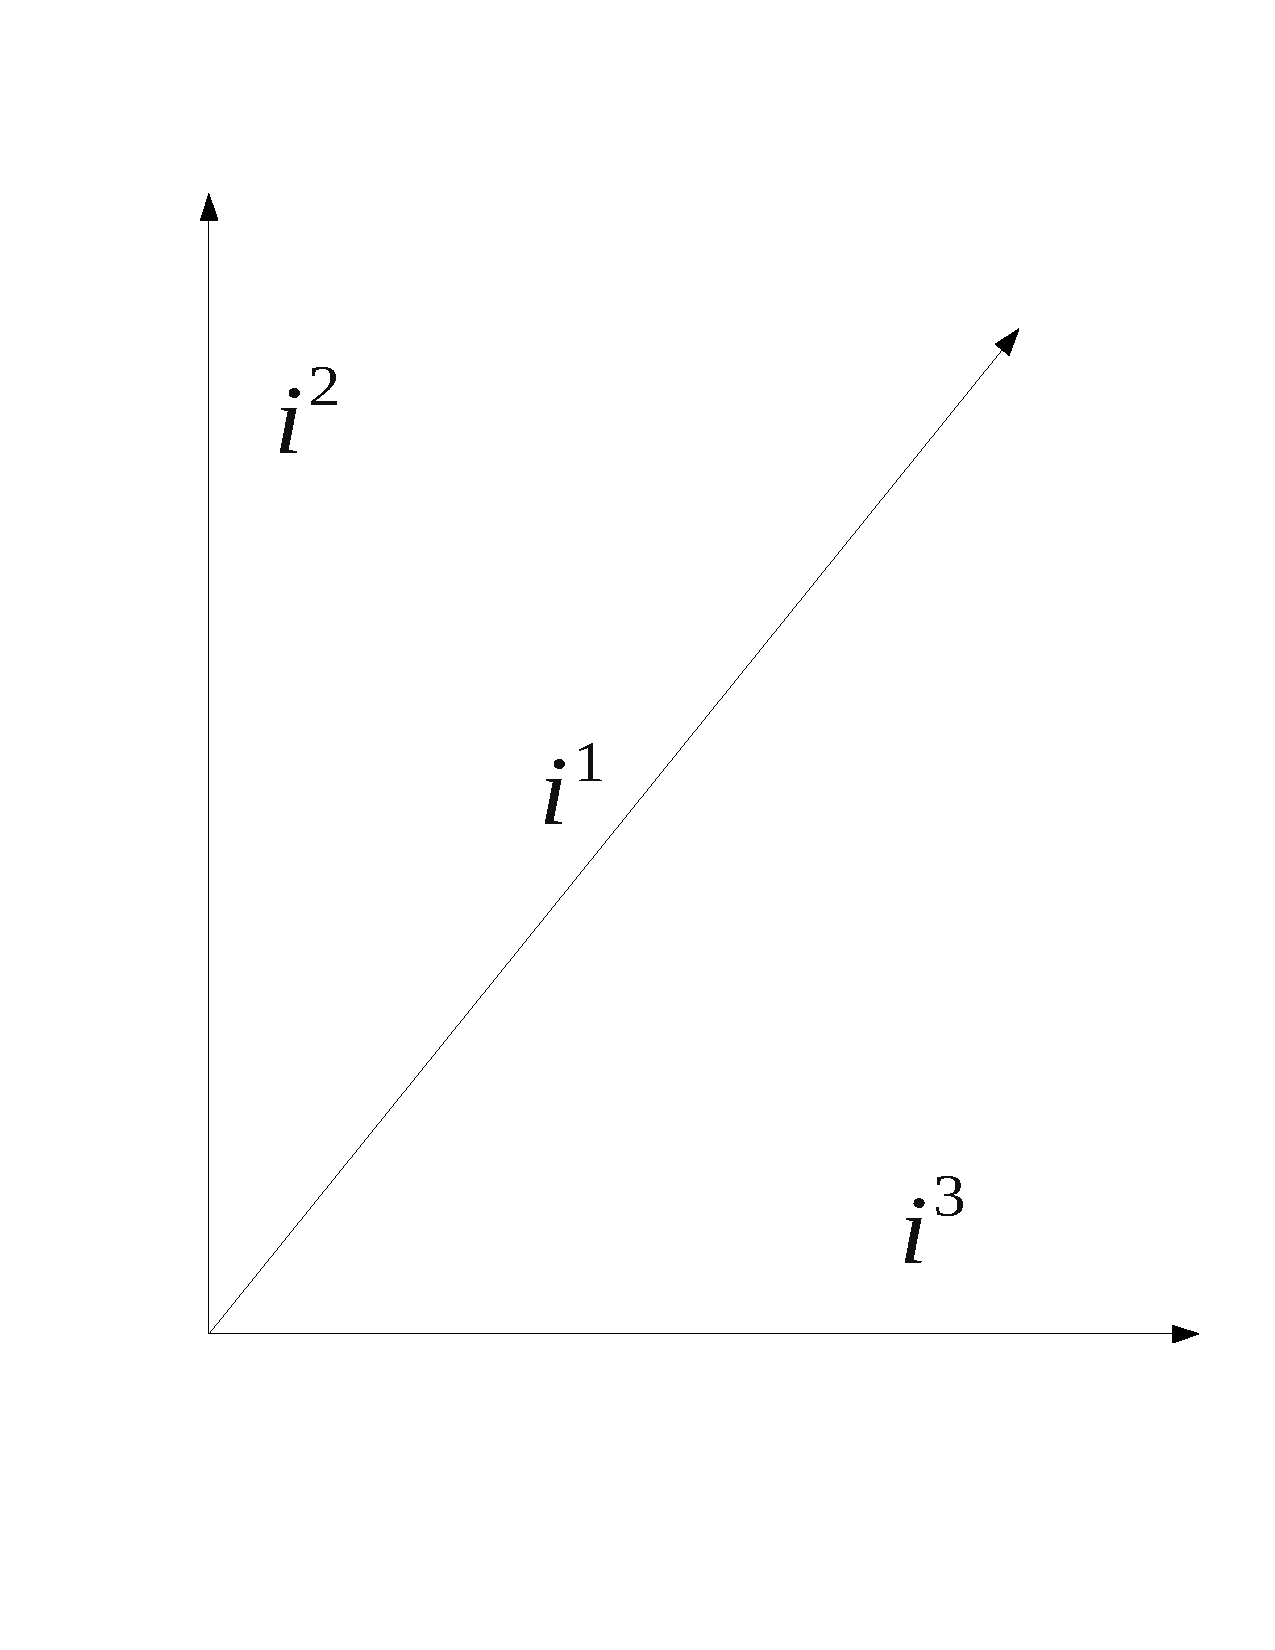
\includegraphics[width=4in,height=3in]{pics/cos-trans-pic.pdf}
\end{center}
\label{fig:no-cos-trans}
\end{figure}

Казалось бы, что значение $\Delta_i = 0,5$ слишком мало, и надо требовать, чтобы
оно стремилось к 1, как было показано на рисунке <<Нарушение транзитивности при использовании меры сходства косинус>> (\ref{exmpl:non-trans-cos}).
Однако такое значение $\Delta_i$ может удовлетворять
реальной РС.
Например, рассмотрим ситуацию, которая может быть характерна
для компании Amazon \cite{amazon-item2item}: объектами являются векторы в
пространстве пользователей, то есть $Y = U, c_Y(i) = (w(1),..,w(m))$
\begin{equation*}
	w(u) =
  \begin{cases}
	1, &\text{если $u \R i$ (пользователь приобрел товар $i$)}\\
	0, &\text{иначе}.
  \end{cases}
\end{equation*}
Данной системой пользуется огромное число человек, поэтому ситуация,
когда товар приобрели, к примеру, 100000 человек, возможна, и вполне
уместно считать товары $i,j$ схожими, если их приобрели более,
чем 49000 одних и тех пользователей.

Для СОМ характерной функцией меры сходства является корреляции Пирсона при
представлении контента пользователя $u$ как выборки
$\{\rho(u,i_0)\}$.

 \begin{equation}
  \du(u, v) =
h \frac{\sum \limits_{i_0 \in P^u_0 \bigcap P^v_0}
	(\rho(u,i_0) - \overline{\rho^u}) \cdot
	(\rho(v,i_0) - \overline{\rho^v})}
	{\sqrt{\sum \limits_{i_0 \in P^u_0}(\rho(u,i_0) -
	\overline{\rho^u})^v \sum \limits_{i_0 \in
	P^v_0}(\rho(v,i) - \overline{\rho^v})^v}}
\end{equation}
В общем случае (при $\Delta_u \in [0,1]$, а не только $\Delta_u = 1$)
коэффициент корреляции не обладает свойством транзитивности
\cite{pearson-trans}, и поэтому в общем случае при применении
данной функции в качестве меры сходства достаточное и необходимое условия не
выполняются.

Если транзитивность в кластере соседей не выполняется, то это приводит
к возрастанию погрешности прогнозной оценки,
так как оценки соседей на прогнозируемый объект могут сильно разниться.

Например, $a = (0,7; 1; 0,1; i_{\bot})$, $u = (0,65; 0,9; 0,1; 1)$,
$v = (0,73; 0,95; 0,05; 0,1)$, $\Delta_u = 0,9$.
Тогда $\du(u_a, u) = 0.9997$, $\du(u_a, v) = 0.9953$, то есть пользователи
$u, v$ попадают в кластер соседей, будучи несхожими
$\du(u, v) = 0.46$. А оценка на неизвестный объект $i_{\bot}$ составляется
из совершенно разных оценок $1$ и $0,1$.
\subsection{Вывод}
Эффективность по критерию качества при применении АКМ для решения задач
зависит от разработчика, а именно от выбора им функционального и тестового
параметра. Не всегда возможно подобрать
функциональный и пороговый параметры так, чтобы выполнялись условия
эффективности решения и реализация РС соответствовала требования
заказчика как, например, в вышеописанном примере для ООМ и $\Delta_u = 0,5$.
АКМ не являются эффективными по критерию качества.
%%%%%%%%%%%%%%%%%%%%%%%%%%%%%%%%%%%%%%%%%%%%%%%%%%%%%%%%%%%%%%%%
%%%%%%%%%%%%%%%%%%%%%%%%%%%%%%%%%%%%%%%%%%%%%%%%%%%%%%%%%%%%%%%%
%%% SPLIP: свойства
%%%%%%%%%%%%%%%%%%%%%%%%%%%%%%%%%%%%%%%%%%%%%%%%%%%%%%%%%%%%%%%%
%%%%%%%%%%%%%%%%%%%%%%%%%%%%%%%%%%%%%%%%%%%%%%%%%%%%%%%%%%%%%%%%
\section{Эффективность по критерию стабильности}
\subsection{Истинность правил вывода}
Правила вывода АКМ, основаны на эвристических
утверждениях. Существующие исследование не анализируют выполнимость этих
утверждений, правила вывода носят аксиоматический характер. Однако,
выполнение эвристических утверждений зависит от свойств исходных данных.
Рассмотрим свойства исходных данных и их влияние на выполнение утверждений.
\subsubsection{Динамика}
В реальности РС работают с динамической информацией,
которая постоянно меняется во времени:
меняется популярность объекта и его восприятие пользователями,
а мощности $U, I$ постоянно растут.
К примеру, новостная система Google News \cite{google-news} ежедневно
пополняет множество объектов, которые являются новостями.

Так же с течением времени меняются потребности и предпочтения пользователей,
поэтому периодически необходимо производить пересмотр их предпочтений \cite{changes}.

Рассмотрим влияние на каждый тип АКМ свойства динамики данных:
\begin{itemize}
	\item утверждение (\ref{assertORS1}) и решение задачи $topN$:
		$(u_a \rt i_0) \wedge (i_0 \rt i) \Rightarrow u_a \R i$.
		Если с течением времени и смене вкусов пользователя меняется отношение
		пользователя к объектам $i_0$ так, что $\rho(u_a,i_0) < \Delta_{\R}$,
		то и $\rho(u_a,i) < \Delta_{\R}$, так как $i_0 \rt i$.
		Таким образом, не выполнится отношение $u_a \R i$, входящее
		в эвристическое утверждение (\ref{assertORS1}), и тогда
		$\eat > \varepsilon_{topN}$, так как цель,
		поставленная при решении задачи $topN$ не будет достигнута. В
		результирующее множество будут входить такие объекты, между которыми и
		активным пользователем не выполняется отношение близости, то есть
		решение неэффективно.

		К примеру, РС интернет-магазина одежды располагает
		данными о покупках пользователя, совершенных зимой. Прибегая к помощи
		системы весной, пользователь, скорее всего, получит в качестве рекомендаций
		зимнюю одежду, хотя планирует выбрать летнюю;

	\item Утверждение СОМ гласит: если в прошлом пользователи были близки по вкусам,
		то и в будущем они будут близки по вкусам. Однако, учитывая динамику
		пользователей, предпочтения пользователей могут смениться так, что
		отношение близости не будет выполняться.

		Если решение будет построено на основании данных некоторого кластера
		$\nup$, и с течением времени предпочтения сменились так, что
		для некоторых $u \in \nup$: $\du(u_a, u) < \Delta_u$, то при
		формировании решения на таком кластере оно будет неэффективным по
		критерию качества, так как нарушится необходимое
		(\ref{suf-cond-pred-srs}) и достаточное (\ref{nec-cond-pred-srs})
		условие: транзитивность отношения близости на кластере.
		Поэтому нужно заново выполнять построение
		кластера, что неэффективно по критерию вычислительной сложности:
		гораздо эффективней единожды сформировать кластер и работать в дальнейшем с
		ним.
\end{itemize}

Таким образом, имеет место быть следующее утверждение.
\begin{assert}
	\label{ass:dynamic}
Если для исходных данных характерно свойство динамики, то
эвристические утверждения могут не выполняться для любого активного
пользователя. И, как следствие, истинность правил вывода нарушается, а решение,
полученные на их основе не являются эффективными по критерию качества решения.
\end{assert}
%Однако, данные, которые были изменены и, тем самым, ухудшают качественность
%результата, могут системой не рассматриваться.
%Если такая информация составляла бОльшую часть контентов,
%то может возникнуть проблема разреженности данных\cite{sparse1, sparse2,
%sparse3}.
%
%Помимо этого, постоянное пополнение множества объектов ведет к проблеме
%добавления нового элемента, следствием
%которого является пересчет матрицы оценок сходства объектов, что, с точки
%зрения вычислительных затрат, является
%дорогим процессом. К примеру, в системе, где есть миллион объектов,
%для добавления нового объекта нужно провести
%миллион операций вычисления оценки сходства.

\subsubsection{Неоднородность предпочтений}
Предпочтения пользователей {\it неоднородны} \cite{psy, hetero-spotify,hetero1}, что означает, что
пользователь может предпочитать совершенно различные объекта, которые не
обязательно являются соседями:
\begin{assert}\label{neodnorodost}
$(u_a \R i) \wedge (u_a \R j) \not \Rightarrow (i \rt j)$.
\end{assert}

Из того, что выполняется $(u_a \R i_0) \wedge (u_a \R i_{\bot})$
нельзя утверждать, что выполняется $i_0 \rt i_{\bot}$, так как значение
$\du(i_0, i_{\bot})$ может быть как больше $\Delta_u$, так и меньше,
в силу того, что вкусы пользователя неоднородны.

К примеру, для кинематографической РС, где характеристиками объектов
являются кинематографические жанры, пользователю могут нравиться как фильм
ужасов $i_0$, так и комедия $i_{\bot}$. Тогда
$(u_a \R i_0) \wedge (u_a \R i_{\bot})$
$\cancel{\Rightarrow} i_0 \rt i_{\bot}$,
так как по кинематографическим жанрам объекты $i_0$ и $i_{\bot}$ не являются
близкими.

Рассмотрим влияние данного свойства:
\begin{itemize}
	\item Рассмотрим ООМ и задачу $topN$. Пусть $P^a_0 = \overline{P}^a_0
		\bigcup \underline{P}^a_0$, где $\overline{P}^a_0$ такое, что $\forall
		i_0,j_0: i_0 \rt j_0, \rho(u_a, i_0), \rho(u_a, j_0) \in
		\overline{P}^a_0$.
		$\underline{P}^a_0$ такое, что $\forall k_0: \di(i_0, k_0) \le \Delta_i$,
		$\rho(u_a, i_0) \in \overline{P}^a_0, \rho(u_a, k_0) \in \underline{P}^a_0$
		Решение (\ref{alg:topn-solve-ors}), реализованное при помощи правила
		вывода ООМ (\ref{ors-pi-top}), применяемым для задачи $topN$
		, будет иметь
		вид $I_{topN} = \{ i: i_0 \rt i \}$,
		если $|\overline{P}^a_0| > |\underline{P}^a_0|$.
		Но тогда в решении существуют две проблема:
		\begin{enumerate}
			\item Рекомендация получается \lq однотипной\rq, так как в
				результирующее множество не попадают объекты, соответствующие
				предпочтениям, которые характерны для объектов типа $k_0$;
			\item Если $P^a_{\bot} = \{ i_{\bot} | k_0 \rt i_{\bot}
				\}$, то вышеприведенное решение будет неэффективным по критерию
				качества $\eit$,
				так как $\eit \rightarrow 1$.
		\end{enumerate}

	\item Рассмотрим CОМ и задачу $pred$.
	Рассмотрим пример данных о пользователе из предыдущего пункта.
	Возможна ситуация, когда
	для такого активного пользователя с неоднородными данными будет составлено
	множество соседей $\{u,v\}$ с односторонними предпочтениями.
	Для пользователя $u$ входное множество данных будет иметь вид
		$\{i_0, u_a, \rho(u_a, i_0)\}: \rho(u_a, i_0) > \Delta_{\R} \}$
		$\bigcup$
		$\{j_0, u_a, \rho(u_a, j_0)\}: \rho(u_a, i_0) = 0 \}$
	Для пользователя $v$ входное множество данных будет иметь вид
		$\{i_0, u_a, \rho(u_a, i_0)\}: \rho(u_a, i_0) = 0 \}$
		$\bigcup$
		$\{j_0, u_a, \rho(u_a, j_0)\}: \rho(u_a, i_0) > \Delta_{\R} \}$

	Пусть $\du = \cos$, тогда возможна ситуация, когда $\du(u, v) = 0$, то есть отношение
	близости $u \ru v$ не выполняется, и поэтому
	нарушается необходимое (\ref{nec-cond-pred-srs}) и
	достаточное (\ref{suf-cond-pred-srs})
	условие эффективного решения по критерию качества.
	\end{itemize}

\begin{assert}
	\label{ass:hetero}
Если для исходных данных характерно свойство неоднородности, то
эвристические утверждения могут не выполняться для любого активного
пользователя. И, как следствие, истинность правил вывода нарушается, а решение,
полученные на их основе не являются эффективными по критерию качества решения.
\end{assert}

Следует отметить, что ООМ, в основном, применяется для задачи $topN$, тогда как
СОМ --- для задачи $pred$. Было показано, что если данные обладают
свойством динамики и неоднородности, то ООМ и СОМ не гарантируют получение
качественного решения.



\subsection{Вывод}
Получение эффективного решения по критерию качества при применении
АКМ зависит от свойств исходных данных, поэтому
\begin{assert}
	\label{input-props-kf}
	АКМ неэффективны по критерию стабильности.
\end{assert}



%Рассмотрим доказательство в более простом случае ---
%при применении средней близости для вычисления
%неизвестного $\rho(u_a,i_{\bot})$\cite{middle-pred}
%$\overline{\rho}(u_a,i_{\bot}) = \frac{1}{|\nup|} \sum
%\limits_{u \in \nup} \rho(u,i_{\bot})$
%, где $\overline{\rho}(u_a,i_{\bot})$ ---
%спрогнозированная близость.
%
%Рассмотрим доказательство для случая, когда $\nup = \{u,v\}$.
%%Пусть $\rho(u_a, i_{\bot}) \ge \overline{\rho}(u_a,i_{\bot})$, тогда
%%% Тут я просто снял модуль и расписал среднее для двух соседей
%%$\rho(u_a,i_{\bot}) - \frac{1}{2}\cdot(\rho(u,i) + \rho(v,i))$.
%Так как $u_a \ru u$, то $|\rho(u_a, i_{\bot}) - \rho(u,i_{\bot})| \le \varepsilon_p$
%по определению \ref{user-sim1}.
%Тогда $\rho(u,i_{\bot}) - \varepsilon_p \le \rho(u_a,i_{\bot}) \le \varepsilon_p +
%% от тут просто подставляю ро(а,и) в исходную разность
%\rho(u,i_{\bot})$. Оценим разницу $A = \rho(u_a,i_{\bot}) -
%\frac{1}{2}\cdot(\rho(u,i) + \rho(v,i))$:\\
%$\frac{1}{2} \cdot (\rho(u,i_{\bot}) - \rho(v, i_{\bot})) \varepsilon_p \le A
%\le \frac{1}{2} \cdot (\rho(u,i_{\bot}) - \rho(v, i_{\bot})) + \varepsilon_p$.
%
%Оценим разность
%$|\rho(u_a,i_{\bot}) - \overline{\rho}(u_a,i_{\bot})| = |\rho(u_a,i_{\bot}) -
%\frac{1}{|\nup|} \sum \limits_{u \in \nup} \rho(u,i_{\bot})|$.
%Так как $u_a \ru u$, то по определению \ref{user-sim1}
%$|\rho(u_a,i_{\bot}) - \rho(u,i_{\bot})| \le \varepsilon_p$, а, значит,
%$\frac{1}{2} \cdot (\rho(u,i_{\bot}) - \rho(v,i_{\bot}) \varepsilon_p
%\ge |\rho(u_a,i_{\bot}) - \overline{\rho}(u_a,i_{\bot})|
%\le \frac{1}{2} \cdot (\rho(u_a,i_{\bot}) - \rho(v,i_{\bot})) + \varepsilon_p$.
%Так как $|\rho(u_a,i_{\bot}) - \overline{\rho}(u_a,i_{\bot})| \le \epsilon_p$,
%то $\rho(u,i_{\bot}) - \rho(v,i_{\bot} \le 2\cdot \epsilon_p +
%2 \cdot \varepsilon_p$


%%%%%%%%%%%%%%%%%%%%%%%%%%%%%%%%%%%%%%%%%%%%%%%%%%%%%%%%%%%%%%%%
%%%%%%%%%%%%%%%%%%%%%%%%%%%%%%%%%%%%%%%%%%%%%%%%%%%%%%%%%%%%%%%%
%%%% SPLIP: применимость етоп
%%%%%%%%%%%%%%%%%%%%%%%%%%%%%%%%%%%%%%%%%%%%%%%%%%%%%%%%%%%%%%%%
%%%%%%%%%%%%%%%%%%%%%%%%%%%%%%%%%%%%%%%%%%%%%%%%%%%%%%%%%%%%%%%%

%\subsection{Необходимое и достаточное условия объективного применения оценок
%эффективности задачи $topN$ при использовании ООМ}
%%% ООМ основаны на эвристических утверждениях, которые выносят предположение относительно
%%% оценки сходства  пользователя и объекта, исходя из схожести только объектов и без введения
%%% соответствующей оценки сходства с область определения $U \bot P$. Это и является основной причиной проблем, которые будут описаны.
%%% Вместо того, чтобы производить непосредственно рассчет $\delta(u_a,i_{\bot})$ РС производят косвенные рассчеты, в основу которых
%%% заложена недоказуемая эвристика.
%Напомним, что целевая задача $topN$ состоит в построении $I_{topn} = \{i: u_a
%\R i\}$.
%Таким образом, по отношению к задаче $topN$, решение
%эффективно по критерию качества, если
%\begin{equation*}
%|\{ i \in \overline{P}^a_{\bot} |u_a \R i \}| = K \ge N \cdot (1 - \varepsilon_{topN})
%\end{equation*}
%Однако, для ООМ проверка выполнения условия $u_a \R i$ основана на
%эвристическом утверждении ООМ \ref{assertORS1}.
%Чтобы показатель $\eit$ соответствовал целевой задаче, нужно, чтобы
%если решение является эффективным по $\eit$, то решение являлось бы эффективным
%и по $\eat$, и наоборот.
%
%То есть должны выполняться следующие два условия:
%\begin{equation}\label{etop-use1}
%\eit \le \varepsilon_{topN} \Rightarrow \eat \le \varepsilon_{topN}
%\end{equation}
%и
%\begin{equation}\label{etop-use2}
%\eat \le \varepsilon_{topN} \Rightarrow \eit \le \varepsilon_{topN}
%\end{equation}
%
%Проанализируем выполнение \ref{etop-use1}.
%Если решение качественно по $\eit$, то
%$\exists I^{\prime}_{topN} \subset I_{topN}, I^{\prime}_{topN} = \{i: \exists
%i_{\bot}, i \rt i_{\bot} \}, |I^{\prime}_{topN}| = K > N \cdot (1 - \varepsilon_{topN}$
%По данным задачи выполняется
%$u_a \R i_{\bot}$, а по решению --- $i \rt i_{\bot}$,
%поэтому, если выполняется утверждение ООМ \ref{assertORS1}, то выполняется отношение
%$u_a \R i$ для $i \in I^{\prime}_{topN}$,
%и тогда значение $\eat < \varepsilon_{topN}$, то есть решение эффективно по критерию
%качества.
%
%Проанализируем выполнение (\ref{etop-use2}). Так как решение эффективно по
%$\eat$, то
%$\exists I^{\prime}_{topN} \subset I_{topN}, I^{\prime}_{topN} = \{i: u_a \R
%i\}, |I^{\prime}_{topN}| = K > N \cdot (1 - \varepsilon_{topN}$
%По данным задачи и по решению известно, что:
%\begin{equation} \label{ors-cond}
%	(u_a \R i_{\bot}) \wedge (u_a \R i)
%\end{equation}
%
%Учитывая утверждение ООМ \ref{assertORS1} и \ref{ors-cond},
%на первый взгляд можно предположить
%выполнение транзитивности отношения близости:
%$\Big((u_a \R i_{\bot}) \wedge (u_a \R i) \Big)  \Rightarrow (i \rt i_{\bot})$.
%Однако утверждение \ref{neodnorodost} показывает, что $ik \rt i_{\bot}$
%может не выполняться при выполнении \ref{ors-cond}.
%Поэтому, если решение качественно по целевой оценке,
%оно может быть {\it неэффективно по оценке} $\eit$, если
%$i \in I^{\prime}_{topN}$, $\du(i, i_{\bot}) \le \Delta_u$ и $|I^{\prime}_{topN}|
%\rightarrow N$, что возможно в силу
%неоднородности предпочтений пользователя.
%
%\begin{assert}
%\label{eit-use}
%Оценка $\eit$ может применяться для определения качества
%решения задачи $topN$ методами ООМ, если выполняется эвристическое утверждение ООМ
%	(assertORS1),
%	что зависит от
%исходных данных.
%\end{assert}

\section{Эффективность по критерию вычислительной сложности}
Вычислительную сложность будем характеризовать асимптотической сложностью
решений, а в качестве элементарной операции возьмем операцию вычисления
значения меры сходства (общую операцию, выполнение которой необходимо для
решения любой задачи при применении любого из правил вывода).

Так как $\Pi_O$ применяется, в основном, для решения задачи $topN$, а
$\Pi_C$ для решения задачи $pred$, то будем рассматривать
асимптотические сложности алгоритмов только для таких случаев.

Асимптотическая сложность алгоритма решения задачи $topN$ при применении
$\Pi_O$ равна $O(n^2)$.
Асимптотическая сложность алгоритма решения задачи $pred$ при применении
$\Pi_C$ равна $O(m)$.

Учитывая огромные мощности множеств $U$ и $I$ при работе реальных РС
с реальными данными и обозначенные асимптотические сложности, для АКМ
имеет место быть проблема масштабируемости \cite{amazon-item2item}, а потому АКМ неэффективны по
критерию вычислительной сложности.

\section{Цели и задачи исследования}
Анализ АКМ выявил следующие открытые проблемы:
		\begin{enumerate}
		\item решение задачи эффективно по критерию качества,
			если выполняются
			эвристические утверждения, что зависит от свойств исходных данных.
			В общем случае, получение качественного решения при применении АКМ
			не гарантировано;
		\item качество решения при применении АКМ зависит
			от следующих параметров системы, которые выбираются разработчиками:
				\begin{enumerate}
					\item функции, которая применяется в качестве меры сходства
				$\du$ для СОМ, $\di$ для ООМ;
		\item порогового значения $\Delta_i, \Delta_u$.
				\end{enumerate}
		\item проблема масштабируемости
		\end{enumerate}

%Цель исследования --- разработка математической модели РС, в которой можно
%более эффективно применять $\Pi_O$ и $\Pi_C$, и определение методов решений во
%введенной модели, не уступающих по эффективности коллаборативным.
%
%Для достижения цели решим следующие задачи:
%\begin{enumerate}
%		\item ввести формальные термины и математические обозначения, в которых определить
%			задачи рекомендательных систем, коллаборативную модель и методы решений
%			задач;
%
%		\item определить критерии оценки эффективности модели и показать, что
%			коллаборативная модель не является эффективной моделью
%			по качеству решения, стабильности и вычислительной сложности;
%
%		\item разработать математическую модель РС, в которой
%
%		\begin{enumerate}
%			\item определить формальные правила вывода, не основанные на
%				эвристических утверждениях;
%			\item определить алгоритмы решения задач, не менее эффективные по
%				по сравнению с алгоритмами
%				коллаборативной модели.
%		\end{enumerate}
%
%	\item реализовать программное обеспечение на основе разработанной модели
%		для демонстрации практического применения разработанной модели;
%
%	\item реализовать программное обеспечение для проведения тестирования
%		коллаборативной и разработанной моделей.
%\end{enumerate}
%

           % Глава 2
\chapter{НЕЧЕТКАЯ МОДЕЛЬ РЕКОМЕНДАТЕЛЬНОЙ СИСТЕМЫ}

% надо перенести на нашу оценку эффективности. То есть мы составляем 
% контент такого пользователя, что расстояние (то есть наша оценка эффективности)
% минимальна
В данной главе описана разработанная в рамках диссертационного исследования
математическая модель РС, основанная на теореии нечетких множеств.
В разработанной модели определены собственные методы решений задач и
обобщенная оценка качества решения.
Проведено теоретическое сравнение эффтиекности разработанной модели
и АКМ по критериям качества решения, вычислительной сложности алгоритмов и
стабильности.
Приведены свойства
разработанной оценки качества, показывающие, что разработанная оценка является
обобщающей оценкой эффективности по критерию качества, которая коррелирует с
суещствующими оценками.

\section{Предпосылки использования теории нечетких множеств}
РС --- гуманистические информационные РС \cite{fuzzy-ponomarev},
работающие с пользователями и их субъективными данными.
При работе с такими данными возникают ситуации неопределенности,
которые можно разделить на две категории:
\begin{enumerate}
\item отсутствие достаточно полного и достоверного знания о предметной области;
\item отсутствие возможности получить исчерпывающую информацию о пользователях
	и объектах.
\end{enumerate}

Существование первой категории неопределенности при работе с АКМ было
продемонстрировано в Главе 2, посвященной анализу АКМ. Было показано, что
эвристические утверждения этой предметной знаний не всегда выполняются, что
свидетельствует об отсутствии полных и достоверных знаний.
В том числе РС оперируют с такими нечеткими, неформальными понятиями, как
<<схож>>, <<обладать тенденцией>>, <<приблизительно равны>> , \lq
вкус>> , <<нравится>> т.п.,
которые точно и формально задать и описать довольно трудно.
Помимо эвристических утверждений, нечеткость присутствует в семантике значений
оценок близостей $\rho(u, i)$. Определить, к примеру, точную семантику между
значением оценки 0,6 и 0,65 довольно трудно, разница между ними размыта.
Вообще говоря, достаточно и полно определить поведение пользователя сложная задача, и
рассчитывать на полноту знаний в этой области не приходится.

Вторая ситуация описывается характерной для РС ситуацией,
которая заключается в разреженности матрицы исходных данных \cite{sparse1, sparse2, sparse3}.
Она определяется тем, что число известных оценок близости по отношение
к числу неизвестных крайне мало. Поэтому для некоторых пользователей
решение задач при помощи правил вывода АКМ невозможно. Или объекты, которые
оценило малое количество пользователей, не будут попадать в результирующее
множество при решении задач при помощи правил вывода АКМ.

Подобные ситуации неопределенности возникают также в экспертных
системах \cite{expert-systems} и в системах принятия решений \cite{set-theory}.
Можно найти некоторое пересечение между экспертными системами и
коллаборатиными РС \cite{cf-expert}. Одним из способов борьбы с
неопределенностью в экспертных системах и системах принятия решений
является применение теории нечетких множеств. Эта же теория была применен
в диссертационной работе для представления исходных данных.

\section{Введение в теорию нечетких множеств}
%ToDo ссылка на клас теорию и булеву логику
% ToDO:эффективным
Классическая теория множеств основана на булевой логике.
Принадлежность элемента некоторому множеству может принимать одно
из двух значений --- $\{0,1\}$ или ({\it истина} или {\it ложь}).
После появления нечетких множеств множества, представляемые при помощи классической теории
стали называть <<жесткими>>. Жесткость представления является источником
проблем при представлении нечетких
понятий при помощи классической теории. В приложении к РС жесткость
заключается в том, что классическая теория может рассматривать,
только два варианта развития событий, к примеру: выполняется ли отношение
близости между пользователем и объектом, или нет.
Такая семантика приемлема для задачи $topN$, так как для ее решения
и требуется определить множество объектов, между которыми и активным
пользователем выполняется отношение близости.
Однако для решения задачи прогнозирования РС должна уметь определять
оценку более гибко: к примеру, идеально, хорошо, удовлетворительно и т.п.

Рассмотрим применение теории нечетких множеств на примере. Предположим,
существует кинематографическая РС,
объектами которой являются фильмы. Характеристики объекта ---
это некоторая неформальная описательная информация.
Предположим, необходимо определить фильмы, которые можно было бы
описать экспертом как <<динамичные>> . В классической
теории множеств множество <<данимичных>>  фильмов $D$ можно было бы составить с
помощью некоторой характеристической функции $f : I \rightarrow D$.
Данную функцию можно было бы задать следующим образом:
\begin{equation*}
  f(i) =
  \begin{cases}
    1, &\text{если для фильма характерен жанр action}\\
    0, &\text{иначе}.
  \end{cases}
\end{equation*}
Представляя все множество <<динамичных>>  объектов $D$, интуитивно
кажется, что границы этого множества должны быть размыты, а
принадлежность элементов этому множеству может быть каким либо образом
ранжирована: можно говорить,
что один фильм динамичнее другого, или столь же динамичен. То есть все
множество $D$ можно упорядочить по свойству динамичности.
Таким образом, можно сказать про конкретный объект множества $D$, что он более
или менее типичен для этой области. К примеру,
фильмы могут обладать несколькими жанрами и могут существовать фильмы, которые
описываются исключительно жанром <<action>> ,
и тогда объект типичен элементу $D$. А могут обладать и нетипичными
жанрами для множества $D$, например
<<drama\rq , что придает драматический эффект и, тем самым, снижает его
динамичность и степень принадлежности множеству $D$.
Следовательно, можно задать некоторую функцию, с помощью которой
можно выразить степень принадлежность элемента к множеству. Пусть
на отрезке $[0,1]$ определена некоторая функция
$d: D \rightarrow [0,1]$, которая сопоставляет элементу $i \in D$ степень
его принадлежности множеству $D$. Если $d(i) = 1$, то можно утверждать, что
объект $D$ типичен для этого множества, если $d(i) = 0$, то можно утверждать, что
объект $D$ нетипичен для этого множества. Промежуточные значения между
$0$ и $1$ являются степенью принадлежности.
Множество $D$ называется нечетким подмножеством универсального множества
$I$, а функция $d$ --- характеристическая функция
принадлежности элементов универсального множества нечеткому подмножеству $D$.

\section{Представление данных в нечеткой модели}
\subsection{Контенты}
Нечеткие множества будем применять для описания информации об объектах и
пользователях системы.
Множество всех возможных характеристик будем называть
универсальным множеством. То есть во введенной терминологии и обозначениях
множество $X$ является универсальным множеством
характеристик пользователей,
а множество $Y$ --- универсальным множеством характеристик объектов.

\begin{defn}
				$c_X(u) = \{(x | w_U(u, x )) \}, w_U(u, x) \in [0,1]$ ---
				контент пользователя, $x \in X$. При этом множество $X$ не
				обязательно является множеством $I$, как в случае с АКМ, а,
				например, в качестве характеристик может выступать контекстная
				информация.
				$w_U(u, x)$ является
				характеристической функции принадлежности.
\end{defn}


\begin{defn}
				$c_Y(i) = \{(y | w_I(i, y )) \}, w_I(i, y) \in [0,1]$ ---
				контент объекта, $y \in Y$.
				$w_I(i, x)$ является
				характеристической функции принадлежности.

\end{defn}

\begin{defn}
				$c_X(u) = \varnothing$, если $w_U(u, x) \equiv 0$ ---
				пустой контент пользователя
\end{defn}

\begin{defn}
				$c_Y(i) = \varnothing$, если $w_I(i, y) \equiv 0$ ---
				пустой контент объекта

\end{defn}

\begin{defn}
	Если пересечение контентов объектов не является пустым контентом, то тогда
	такие элементы будем называть {\it сравнимыми}.
\end{defn}

\subsection{Основные операции над контентами}
Теория нечетких множеств позволяет определить такие операции над контентами,
как их пересечение, объединение и дополнение, так как контенты
являются нечеткими подмножествами. Данные операции будут применены в дальнейшем.
\begin{defn}
	Пересечение контентов пользователей $u_1$ и $u_2$, заданных на универсальном множестве характеристик
	$X$, --- это наибольшее нечеткое множество $c_X(v) = c_X(_1u)
	\bigcup c_X(u_2)$,
	содержащееся одновременно и в $c_X(u_1)$, и в $c_X(u_2)$,
	с функцией принадлежности $w_U$, заданной следующей формулой:
\end{defn}

\begin{equation}
				c_X(u_1) \bigcap c_X(u_2) = c_X(v): \forall x \in X w_U(v, x) =
				\min(w_U(u_1, x), w_U(u_2, x))
\end{equation}

\begin{defn}
	Пересечение контентов объектов $i_1$ и $i_2$, заданных на
	универсальном множестве характеристик
	$Y$, --- это наибольшее нечеткое множество
	$c_Y(j) = c_Y(i_1) \bigcup c_Y(i_2)$,
	содержащееся одновременно и в $c_Y(i)$, и в $c_Y(j)$,
	с функцией принадлежности, заданной следующей формулой:
\end{defn}
\begin{equation}
				c_Y(i_1) \bigcap c_Y(i_2) = c_Y(j): \forall y \in Y w_I(j, y) =
				\min(w_I(i_1, y), w_I(i_2, y))
\end{equation}

\begin{defn}
Объединение контентов пользователей $u_1$ и $u_2$,
	заданных на универсальном множестве $X$, --- это наименьшее
	нечеткое множество $c_X(v) = c_X(u_1) \bigcap c_X(u_2)$,
	включающее как $c_X(u_1)$, так и $c_X(u_2)$ с функцией
	принадлежности, заданной следующим образом:
\end{defn}
\begin{equation}
				c_X(u_1) \bigcup c_X(u_2) = c_X(v): \forall x \in X w_U(v, x) =
				\max(w_U(u_1, x), w_U(u_2, x))
\end{equation}

\begin{defn}
Объединение контентов объектов $i_1$ и $i_2$,
	заданных на универсальном множестве $Y$, --- это наименьшее
	нечеткое множество $c_Y(j) = c_Y(i_1) \bigcap c_Y(i_2)$,
	включающее как $c_Y(i_1)$, так и $c_Y(i_2)$ с функцией
	принадлежности, заданной следующим образом:
\end{defn}
\begin{equation}
				c_Y(i_1) \bigcup c_Y(i_2) = c_Y(j): \forall y \in Y w_I(j, y) =
				\max(w_I(i_1, y), w_I(i_2, y))
\end{equation}



%\begin{defn}
%Пусть $u^1$ и $u^2$ --- контенты пользователей. Говорят, что контенты $u^1$ и $u^2$ являются дополнением друг друга, если $u^1 = \overline{u^2}$ и $u^2 = \overline{u^1}$, 
%если $\forall$ $x \in X$ $w_U_1(x) = 1 - w_U_2(x)$
%\end{defn}
%
%\begin{defn}
%Пусть $i^1$ и $i^2$ --- контенты пользователей. Говорят, что контенты $i^1$ и $i^2$ являются дополнением друг друга, если $i^1 = \overline{i^2}$ и $i^2 = \overline{i^1}$, 
%если $\forall$ $y \in Y$ $w_I_1(y) = 1 - w_I_2(y)$
%\end{defn}

%ToDo показать на примере взаимосвязь. Вычислить косинус например и расстояние Хэмминга
%TODO: cite fuzzy logic
\section{Расстояние между пользователями и расстояние между объектами}
В разработанной модели будем пользоваться не мерой сходства, а
расстоянием. На основании значений расстояний будем определять,
выполняется отношение близости, или нет. Расстояние противоположно по
поведению и по семантике мере сходства. Там, где мера сходства растет,
расстояние убывает.

Введем расстояние между пользователями
$\rhu: U \times U \rightarrow [0,1]$ и объектами $\rhi: I \times I \rightarrow
[0,1]$ как обобщенное расстояние Хэмминга.

Расстояние между пользователями:
    \begin{equation}
		\label{fuz:rhu}
		\rhu(u,v) =
      \begin{cases}
		  \text{Не определено, если} & c_X(u) \bigcap c_X(v) = \varnothing\\
		  \frac{1}{|X|} \cdot \sum \limits_{x \in X} |w_U(u, x) -
		  w_U(v,x)| & \text{иначе}
      \end{cases}
    \end{equation}

Расстояние между пользователями:
    \begin{equation}
		\label{fuz:rhi}
		\rhi(i, j) =
      \begin{cases}
         \text{Не определено, если} & c_Y(i) \bigcap
		  c_Y(j) = \varnothing \\
        \frac{1}{|Y|} \cdot \sum \limits_{y \in Y} |w_I(i, y) - w_I(j,y)| & \text{иначе}
      \end{cases}
    \end{equation}

\subsubsection{Метрические свойства расстояния}
\begin{trm}
	\label{metric}
	Введенные функции $\rhi$ (\ref{fuz:rhi}) и $\rhu$ (\ref{fuz:rhu})
	обладают метрическими свойствами на подмножестве сравнимых агентов.
\end{trm}
Покажем выполнение метрических свойств для $\rhu$.
Доказательство для $\rhi$ проводится аналогично
с заменой соответствующих обозначений.

Опишем метрические свойства \cite{matan} и покажем выполнение каждого из них:
\begin{enumerate}
\item Положительность: $\rhu(u,v) \ge 0$
\item Симметричность: $\rhu(u,v) = \rhu(v,u)$
\item Неравенство треугольника: $\rhu(u, v) \le \rhu(u,z) + \rhu(v,z)$
\end{enumerate}
Выполнение свойства (1): $\rhu(u,v) = \frac{1}{|X|}
\cdot \sum \limits_{x \in X} |w(u,x) - w(v,x)|$. Каждый
элемент $|w(u,x) - w(v,x)| \ge 0$, а сумма неотрицательных
элементов неотрицательна.

Выполнение свойства (2): $\rhu(v,u) = \frac{1}{|X|} \cdot \sum \limits_{x \in X} |w_U(v,x) - w_U(u,x)| =
\frac{1}{|X|} \cdot \sum \limits_{x \in X} |w_U(u,x) - w_U(v,x)| = \rhu(u,v)$.

Выполнение свойства (3): докажем выполнение этого свойства с помощью метода математической индукции. Индукция по мощности $X$.
Рассмотрим его выполнение для $|X| = 1$. Рассмотрим пользователей $v,z$.
Так как $|X| = 1$, неравенство треугольника $\rho(v,z)$ запишется в виде

\begin{equation}\label{triangle-proof1}
|w_U(u,x) - w_U(v,x)| \le |w_U(u,x) - w_U(z,x)| + |w_U(v,x) - w_U(z,x)|
\end{equation}
Раскроем \ref{triangle-proof1} для каждой возможной ситуации:
\begin{itemize}
% z v u
	\item Пусть $(w_U(u,x) \ge w_U(v,x))$ $\wedge$ $(w_U(v,x) \ge w_U(z,x))$.
Тогда  неравенство \ref{triangle-proof1} примет следующий вид:
$w_U(u,x) - w_U(v,x) \le w_U(v,x) - w_U(z,x) + w_U(v,x) - w_U(z,x)$, то есть
$w_U(v,x) \ge w_U(z,x)$, что является истиной;


% v z u
\item Пусть $(w_U(u,x) \ge w_U(z,x))$ $\wedge$ $(w_U(z,x) \ge w_U(v,x))$.
Тогда  неравенство \ref{triangle-proof1} примет следующий вид:
$w_U(u,x) - w_U(v,x) \le w_U(u,x) - w_U(z,x) + w_U(z,x) - w_U(v,x)$, то есть
$w_U(z,x) \ge w_U(v,x)$, что является истиной;

% z u v
\item Пусть $(w_U(v,x) \ge w_U(u,x))$ $\wedge$ $(w_U(u,x) \ge w_U(z,x))$.
Тогда  неравенство \ref{triangle-proof1}
примет следующий вид:
	$w_U(v,x) - w_U(u,x) \le w_U(u,x) - w_U(z,x) + w_U(v,x) - w_U(z,x)$, то
		есть $w_U(u,x) \ge w_U(z,x)$, что является истиной;

% u z v
	\item Пусть $(w_U(v,x) \ge w_U(z,x))$ $\wedge$ $(w_U(z,x) \ge w_U(u,x))$.
Тогда  неравенство \ref{triangle-proof1}
примет следующий вид:
	$w_U(v,x) - w_U(u,x) \le w_U(z,x) - w_U(u,x) + w_U(v,x) - w_U(z,x)$, то
		есть $0 \ge 0$, что является истиной;

% v u  z
\item Пусть
	$(w_U(u,x) \ge w_U(v,x))$ $\wedge$ $(w_U(z,x) \le w_U(u,x))$.
Тогда  неравенство \ref{triangle-proof1} примет следующий вид:
		$w_U(u,x) - w_U(v,x) \le w_U(z,x) - w_U(u,x) + w_U(z,x) - w_U(v,x)$, то
		есть
		$w_U(z,x) \ge w_U(u,x)$, что является истиной;

% u v  z
\item Пусть
	$(w_U(v,x) \ge w_U(u,x))$ $\wedge$ $(w_U(z,x) \le w_U(v,x))$.
Тогда  неравенство \ref{triangle-proof1} примет следующий вид:
		$w_U(v,x) - w_U(u,x) \le w_U(z,x) - w_U(u,x) + w_U(z,x) - w_U(v,x)$, то
		есть
		$w_U(z,x) \ge w_U(v,x)$, что является истиной;
\end{itemize}

Пусть утверждение верно для $|X| = k$. Докажем, что утверждение верно
для $|X| = k + 1$. В этом случае неравенство треугольника запишется в следующем
виде: \\
$\frac{1}{k+1} \cdot \Big(\sum \limits_{l=1}^{k} |w_U(u,x_l) - w_U(v,x_l)| +
|w_U(u,x_{k+1}) - w_U(v,x_{k+1})| \Big)\le$ \\
$\Big(\frac{1}{k+1} \cdot \sum \limits_{l=1}^{k} |w_U(v,x_l) - w_U(z,x_l)| +
|w_U(v,x_{k+1}) - w_U(z,x_{k+1})|\Big) +$\\
$\Big(\frac{1}{k+1} \cdot \sum \limits_{l=1}^{k} |w_U(u,x_l) - w_U(z,x_l)| + |w_U(u,x_{k+1}) - w_U(z,x_{k+1})|\Big)$.

Так как утверждение выполняется для $|X| = k$, то\\
$\frac{1}{k+1} \Big(\sum \limits_{l=1}^{k} |w_U(v,x_l) - w_U(z,x_l)| + \sum \limits_{l=1}^{k} |w_U(u,x_l) - w_U(z,x_l)| -
\sum \limits_{l=1}^{k} |w_U(u,x_l) - w_U(v,x_l)|\Big) = A \ge 0$. Тогда неравенство треугольника для $|X| = k + 1$ запишется в виде
$|w_U(u,x_{k+1}) - w_U(v,x_{k+1})| \le |w_U(v,x_{k+1}) - w_U(z,x_{k+1})| + |w_U(v,x_{k+1}) - w_U(z,x_{k+1})| + A$.
Неравенство
$|w_U(u,x_{k+1}) - w_U(v,x_{k+1})| \le |w_U(v,x_{k+1}) - w_U(z,x_{k+1})| +
|w_U(v,x_{k+1}) - w_U(z,x_{k+1})|$ является верным по доказательству,
приведенному для $|X| = 1$.
Тогда $|w_U(u,x_{k+1}) - w_U(v,x_{k+1})| \le |w_U(v,x_{k+1}) - w_U(z,x_{k+1})|
+ |w_U(v,x_{k+1}) - w_U(z,x_{k+1})| + A$, так как $A$ --- неотрицательное число.

\section{Отношение близости пользователей и отношение близости объектов}
Определим отношение близости объектов:
\begin{equation}\label{rt}
  i \rt j \Leftrightarrow \overset{i}{\rho}(i,j) = 0
\end{equation}
Определим отношение близости пользователей:
\begin{equation}\label{ru}
	u \ru v \Leftrightarrow \overset{u}{\mathcal{\rho}}(u,v) \le
	\varepsilon_p
\end{equation}

По своей сути метрические функции расстояния являются количественными
показателями сходства элементов некоторого множества. Поэтому, отношения
близости, заданные через формулу расстояния могут считаться объективными.
При этом, если в РС используются меры сходства, высокий показатель которых
соответствует выполнению отношения близости, то тогда верны следующие теоремы:

\begin{trm}
	Отношение близости объектов, заданное в нечеткой модели (\ref{rt}), соответствует
	отношению близости объектов, заданному в ООМ (\ref{rt-ors}).
\end{trm}

Если $i \rt j$ в разработанной модели (\ref{rt}),
то $\rho(i, j) = 0$, и тогда $\di(i, j) = 1$, так как $i =
j$ и в РС используются симметричные меры сходства (использование
асимметричных мер сходства не имеет смысла). Так как $\di(i, j) =
1$, то $i \rt j$ для любого $\Delta_i$.

Рассмотрим следующий пример: $\di(i,j) = cos(\angle(i,j))$
и пусть $|c_Y| = 2$. Пусть $i, j$ такие, что $\rhi(i, j) = 0$, то есть
$w_I(i,y) = w_I(j,y)$. Тогда $\di(i, j) =
\frac{
	w_I(i,y_1) \cdot (w_I(i,y_1) +
	w_I(j,y_2) \cdot (w_I(j,y_2)
	} {
		\sqrt{w_I(i,y_1)^2 + w_I(i,y_2)^2} \cdot
		\sqrt{ (w_j(i,y_1))^2 + (w_I(j,y_2))^2   }
	} =
\frac{
	w_i(i,y_1) \cdot (w_i(i,y_1) +
	w_i(i,y_2) \cdot (w_i(i,y_2)
	} {
		\sqrt{w_i(i,y_1)^2 + w_i(i,y_2)^2} \cdot
		\sqrt{ (w_i(i,y_1))^2 + (w_i(i,y_2))^2   }
	} = 1$.
То есть $i \rt j$ для любого $\Delta_i$.

\begin{trm}
	Отношение близости пользователей, заданное в нечеткой модели (\ref{ru}), соответствует
	отношению близости пользователей, заданному в СОМ (\ref{user-sim1}).
\end{trm}

В СОМ $X = I$, $w_U(u, i) = \rho(u, i)$. Покажем, что если
отношение близости выполняется в нечеткой модели, то между пользователями
выполняется отношение близости в СОМ.
Докажем теорему методом индукции.
Пусть $n = 1$. Тогда
$u \ru v \Rightarrow |\rho(u, 1) - \rho(v, 1)| \le
\varepsilon_p$,
что полностью соответствует определению пользователей, между
которыми выполняется отношение близости (\ref{user-sim1}).

Пусть утверждение верно для $n = k$, то есть $\frac{1}{k} \cdot \sum
\limits_{i=1}^k|\rho(u, i) - \rho(v, i)| \le \varepsilon_p$.

Покажем, что теорема верна для $n = k + 1$.
$\rho(u, v) = \frac{1}{k + 1} \cdot \sum \limits_{i=1}^{k+1} |\rho(u,i) -
\rho(v,i)| \le $
$\varepsilon_p + \frac{1}{k + 1} \cdot |\rho(u, k+1) -
\rho(v, k+1)| \le \varepsilon_p$. Получаем, что
$|\rho(u, k+1) - \rho(v, k+1)| = 0$,
что соответствует формуле
(\ref{user-sim1}).
%Расстояние обладает противоположной семантикой семантике меры сходства, и там, где

%расстояние убывает, оценки сходства растет. Определим корреляцию между мерой
%сходства и расстоянием следующим образом:
%\begin{equation}\label{rho-sim}
%\rhi(i,j) = 1 - \di(i,j),
%\rhu(u,v) = 1 - \du(u,v)
%\end{equation}
%Введенная взаимосвязь является очень простой, однако
%она описывает ситуацию, когда $\rhi(i,j) = 0$, то контенты таковы, что, скорее
%всего, используемая мера сходства, например, косинус будет равна 1.
%но она выражает тот факт, что
%если 
%
%Данное уравнение следует из того факта, что для одинаковых элементов применямые
%оценки сходства приобретают значение, равное 1, а расстояния --- 0.
%
%TODO: ВЕЗДЕ УБРАТЬ 1 - \Delta, если речь идет о значении расстояния. Оно должно принадлежать окрестности.
%\subsection{Свойства отношения близости}
%В Главе 1 говорилось о важности выполнения свойства транзитивности отношения
%близости и было показано, что для КРТ выполнение этого свойства не
%гарантируется.
%Рассмотрим выполнение этого свойства в контентной модели.
%\begin{trm}\label{trans-rho}
%Отношения $\rt$, $ru$ в контентной модели обладает свойством транзитивности.
%\end{trm}
%
%Докажем выполнение свойства транзитивности отношения $\rt$. Доказательство
%свойства транзитивности для $\ru$ проводится аналогично.
%Выше было показано, что выполняется неравенство треугольника для введенных
%расстояний.
%Рассмотрим некоторые объекты $1, 2, 3$.
%Пусть $1 \rt 2$ $\wedge$ $2 \rt 3$. Так как функция
%обладает метрическими свойствами, то $\rhi(1,3) \le \rhi(1, 2) + \rhi(2, 3)$.
%Для любой сколь угодно малой окрестности $\varepsilon(0)$ можно составить такую окрестность $\xi(\varepsilon)$, что:
%\begin{enumerate}
%\item $\forall$ $\varepsilon_1$, $\varepsilon_2$ $\in \varepsilon(0)$ выполняется, что
%$\varepsilon_1+\varepsilon_2 \in \xi(\varepsilon)$.
%\item При $\varepsilon(0) \rightarrow 0 \Rightarrow \xi(\varepsilon) \rightarrow 0$.
%\end{enumerate}
%Тогда для любых $\rhi(1, 2)$ и $\rhi(2, 3)$ значение $\rhi(1,3) \in \xi(\varepsilon)$.
%В пределе, при $\varepsilon(0) \rightarrow 0$ получим, что и $\rhi(1,3) \rightarrow 0$, следуя свойству (2) окрестности
%$\xi(\varepsilon)$, то есть $\rhi(1,3) \le \epsilon_0 \in \varepsilon(0)$.
%То есть выполняется $1 \mathcal{R} 3$, а значит выполняется свойство транзитивности.

%% %
%% % ОЦЕНКА ЭФФЕКТИВНОСТИ
%% %
%% \section{Оценка эффективности $\mathcal{E}$}
%% %ToDo: расписать конкретно для полноты, не как f( от числа ), для точности, потом для кривой точность-полнота
%% % ну или сказать. Ну, или как-то потом обощить на другие оценки эффективности. Сказать, что все они f( от мощности )
%% % 
%% В разделе <<Анализ коллаборативных РС\rq  было показано, что не всегда существующие оценки эффективности
%% могут быть применены для выявление эффективности решения основных задач РС. В данном разделе предложен способ
%% введения оценки эффективности, основанный на использовании расстояния между пользователем и объектом. Свойства данного способа 
%% оценки эффективности показаны далее. 

%% Пусть мы обладаем алгоритмом, вычисляющим $\rho_{1}(u^a, t_{1})$ по контентам пользователя и объекта так, что:
%% \begin{equation}
%% |\rho_1(u^a,t_{1}) - \rho_{1}(u^a,t_{1})| \in \varepsilon(0), t_{1} \in T_{\times}
%% \end{equation}
%% где $\rho_{1}$ является {\it метрической функцией расстояния}. При этом будем считать, что значение поставленной оценки связано с расстоянием следующим образом:
%% $\rho_1(u^a, i^l) = 1 - \delta(u^a, i^l)$. Напомним так же, что $e^1 \mathbf{R} e^2 \Leftrightarrow \delta(e^1,e^2) > \Delta, e^i \in \{U,T\} \Leftrightarrow \rho_1(e^1,e^2) < 1 - \Delta$.

%% Характеристиками пользователя могут выступать не только его оценки. К примеру,
%% пользователь перед работой с РС может заполнить анкету \cite{bank}, которая состоит из характеристик, принадлежащих также и объектам, или из характеристик,
%% которые сопоставимы с характеристиками объектов. К примеру, это может набор кинематографических жанров, которые интересны пользователю и 
%% характерны для фильмов.  
%% При наличии алгоритма расчета $\rho_{1}(u^a, i^l)$, мы можем провести вычисление эффективности результатов 
%% по алгоритму, представленному в следующем алгоритме.
%% % ToDo в статье про полноту алгоритм сменен. Получается два разных упорядочвания. На этом надо заострить внимание.
%% \begin{algorithm}
%% \caption{Вычисление оценки эффективности $\mathcal{E}$}
%% \begin{algorithmic}[1]
%% \State Читаем тестовое множество $I^a_{\times}$
%% \State Читаем результирующее множество $I^a_{1}$
%% \State Упорядочиваем тестовое множество $I^a_{\times}$ по возрастанию $\rho_1(u^a, t_{\times})$, где 
%% $\rho_1(u^a, t_{\times})$ --- известная величина, равная $1 - \delta(u^a, t_{\times})$
%% \State Упорядочиваем тестовое множество $I^a_{1}$ по возрастанию $\rho_{1}(u^a, t_{1})$, где 
%% $\rho_{1}(u^a, t_{1})$ --- вычисленная величина. 
%% \State $\mathcal{E} = 0$
%% \For{$i = 1, i \le N$} \Comment{Для каждого $i$-ого объекта результирующего множества вычислим погрешность оценки и просуммируем общую погрешность результата.}
%% \State $\mathcal{E} = \mathcal{E} + |\rho_1(u^a, i^i_{\times}) - \rho_{1}(u^a, i^i_{1})|$
%% \State $i = i + 1$
%% \EndFor
%% \State $\mathcal{E} = \frac{1}{N} \cdot \mathcal{E}$
%% \end{algorithmic}
%% \end{algorithm}

%% То есть для оценки эффективности вычисляется значение следующей функция:
%% \begin{equation}
%% \mathcal{E} = \frac{1}{N} \cdot  \sum \limits_{i=1}^N |\rho_{1}(u^a, i^i_{1}) - \rho_1(u^a, i^i_{\times})|,
%% \end{equation}

%% При этом множества $I^a_{\times}, I^a_{1}$ должны быть упорядочены по возрастанию значения расстояния $\rho_1(u^a, i^i_{\times})$ и
%% $\rho_{1}(u^a, i^i_{1})$ соответственно. Данная оценка расчитывет, насколько далеко объект в позиции $i$ результирующей выборки
%% отстоит по значению $\rho_1(u^a,i^i_{\times})$ от реальной ситуации.

%% Так как алгоритм вычисления $\rho_{1}(u^a, i^i_{1})$ обладает тем свойством, что вычисленное значение близко к реальному, то предложенный 
%% способ оценки заменяет процесс, когда пользователь сам поставит оценку $\delta_{1}(u^a, i^i_{1})$ рекомендованному объекту и 
%% вычислит его <<отдаленность\rq   --- то есть расстояние --- от своих предпочтений.

%% Такой способ оценки аннулирует проблемы, связанные со свойствами данных. Это связано с тем, что введенная оценка эффективности --- функция от вычисленной величины
%% $\delta_{1}(u^a, t_{1} \in I^a_{1})$ и известной $\delta(u^a, t_{\times} \in I^a_{\times})$, на которые не накладываются дополнительные условия, 
%% зависящие от данных. В отличии от оценки точности $\mathcal{E}_{\top}$ и $\mathcal{E}_p$, когда вычисленные и известные величины связаны эвристическими утверждениями ОРС и СРС, выполнение которых зависит от входных данных.
%% Таким образом, способ разбиения входного множества на тестовое и обучающее никак не влияет на значение оценки эффективности $\mathcal{E}$.
%% Значение этой оценки зависит от способа задания контентов пользователей, объектов и точности сопоставления характеристик пользователей
%% с характеристиками объектов.

%% Основывая выводы об эффективности решения не на косвенных признаках сходства объектов, а на вычислении актуального на данный момент времени\footnote{
%% При условии, что актуальные данные введены в систему пользователем. Это может быть обеспечено, 
%% к примеру, обязательным условием заполнением анкеты перед запросом на нахождение топового списка объектов.}
%% значения $\delta_{1}(u^a,t_{1})$, аннулируются проблемы, связанные с динамикой данных и их неоднородностью. 

%% Идеальным решением по $\mathcal{E}$ назовем $I^a_{1} = \{ i^l_{1}, \rho_{1}(u^a,i^l) \}$: 
%% $|\rho_{1}(u^a, i^l_{1}) - \rho_1(u^a, i^l_{\times})| \in \varepsilon(0)$. Будем говорить, что решение эффективно по $\mathcal{E}$, если
%% $|\rho_{1}(u^a, i^l_{1}) - \rho_1(u^a, i^l_{\times})| \in \varepsilon(0)$, $l=1..K \rightarrow N$.

%% %% Помимо точности существует ряд других оценок эффективностей решения, принадлежащих к разным классам. В связи с наличием многообразия оценок
%% %% у исследователей РС возникают вопросы: как сравнивать результаты, которые были оценены не коррелирующими оценками сходства, 
%% %% какую оценку сходства выбрть, как сравнить алгоритмы, протестированные на различных входных данных.

%% \section{Свойства оценка эффективности $\mathcal{E}$}
%% Назовем множество входных данных $I^a = \{ (i^l,\delta(u^a,i^l))| \delta(u^a,i^l) > \Delta \}$ 
%% (и в том числе $I^a_0,I^a_{\times})$) {\it репрезентативным}, если $\underset{l \rightarrow \infty} {\mathrm{\lim}}$  
%% $|\overline{\delta} - \delta(u^a,i^l)| = 0$, где $\overline{\delta}$ --- среднее значение оценок пользователя. 
%% То же распространяется и на расстояние: $\underset{l \rightarrow \infty} {\mathrm{\lim}}$  
%% $|\overline{\rho} - \rho_1(u^a,i^l)| = 0$
%% %Заметим, что  
%% %данные для задачи top-$N$ имеют свойство, что $\forall$ $(i^l, \delta(u^a,i^l))$: 
%% %$\delta(u^a,i^l)) > \Delta$.

%% \section{Применимость оценки эффективности $\mathcal{E}$ к целевой задаче top-$N$}
%% %ToDo: ВСЮ ПРИМЕНИМОСТЬ ПЕРЕПИСАТЬ, ЧТОБЫ НЕ БЫЛО 1 - \Delta
%% \begin{assert}
%%   Оценка эффективности $\mathcal{E}$ удовлетворяет целевой задаче top-$N$.
%% \end{assert}

%% {\bf Покажем, что} $\mathcal{E} \le \varepsilon_0 \Rightarrow \mathcal{E}_A \le \varepsilon_0$:
%% \begin{enumerate}
%% \item $\mathcal{E} \le \varepsilon_0 \Rightarrow |\rho_1(u^a, i^i_{\times}) - \rho_{1}(u^a, i^i_{1})| \in \varepsilon(0), i=1..K, K \rightarrow N$.
%% Решение эффективно при условии, что разница расстояния мала для числа $K \rightarrow N$.
%% \item По данным задачи выполняется $\forall$ $i^i:$ $\rho_1(u^a, i^i_{\times}) < 1 - \Delta$, а, учитывая пункт (1) доказательства, получим, что 
%% $\rho_{1}(u^a, i^i_{1}) < 1 - \Delta$ для $i=1..K, K \rightarrow N$
%% \item Учитывая (11) и следствие пункта (2), получим, что $\rho_1(u^a, i^i_{1}) < 1 - \Delta$ для $i=1..K, K \rightarrow N$
%% %ToDo: перееписать как в статье
%% \item $\delta(u^a, i^i_{1}) = 1 - \rho_1(u^a, i^i_{1}) \Rightarrow \delta(u^a, i^i_{1}) > \Delta$ для $i=1..K, K \rightarrow N$ $\Rightarrow$
%% $\mathcal{E}_A < \varepsilon_0$
%% \end{enumerate}
%% %ToDO: Далее хороший момент, что в пределе будет насрать на дельта, надо и его расписать.
%% %% а при $\varepsilon(0) \rightarrow 0$ 
%% %% $\delta(u^a, i^i_{1}) \rightarrow 1$, а значит $\delta(u^a, i^i_{1}) > \Delta$ для любого $\Delta \in [0,1]$. 
%% %% Поэтому при $\varepsilon(0) \rightarrow 0$  


%% {\bf Покажем, что} $\mathcal{E}_A \le \varepsilon_0 \Rightarrow \mathcal{E} \le \varepsilon_0$:
%% \begin{enumerate}
%% \item $\mathcal{E}_A < \varepsilon_0$ $\Rightarrow$ $\delta(u^a, i^i_{1}) > \Delta$ для $i=1..K, K \rightarrow N \Rightarrow \rho_1(u^a, i^i_{1}) < 1 - \Delta$

%% \item $|\rho_1(u^a, i^i_{1}) - \rho_{1}(u^a, i^i_{1})| \in \varepsilon(0) \wedge$
%% $\rho_1(u^a, i^i_{1}) < 1 - \Delta \Rightarrow \rho_{1}(u^a, i^i_{1}) < 1 - \Delta$ для $i=1..K, K \rightarrow N$

%% \item Оценим $|\rho_1(u^a, i^i_{\times}) - \rho_{1}(u^a, i^i_{1})|$: обе величины меньше $1 - \Delta$ и, учитывая репрезентативность множеств,
%% получим, что $\underset{i \rightarrow \infty} {\mathrm{\lim}}$  
%% $|\rho_1(u^a, i^i_{\times}) - \rho_{1}(u^a, i^i_{1})| = 0 \Rightarrow \mathcal{E} < \varepsilon(0)$ для больших величин $N$

%% %% \item Учитывая репрезентативность, получаем, что:\\ $\mathcal{E}_A < \varepsilon_0$ $\Rightarrow$ $|\overline{\delta} - \delta(u^a, i^i_{1})| \in \varepsilon(0)$ 
%% %% для $i=1..K, K \rightarrow N$, где $\overline{\delta} = \frac{1}{M} \cdot \sum \limits_{t_0 | u^a \mathbf{R} i^l} \delta(u^a,t_0)$. $\overline{\delta}$ --- средняя высокая 
%% %% оценка активного пользователя, поставленная им понравившимся ему объектам.

%% %% \item $|\overline{\delta} - \delta(u^a, i^i_{1})| = |(1 - \overline{\delta}) - (1 - \delta(u^a, i^i_{1}))| = \overline{\rho} - \rho_1(u^a, i^i_{1})$

%% %% \item $\mathcal{E}_A < \varepsilon_0$ $\Rightarrow$ $|\overline{\rho} - \rho_1(u^a, i^i_{1})| \in \varepsilon(0)$ для $i=1..K, K \rightarrow N$

%% %% \item Из условия $|\overline{\rho} - \rho_{1}(u^a, i^i_{1})| \in \varepsilon(0)$ для $i=1..K, K \rightarrow N$ и (9) следует, что $\mathcal{E} < \varepsilon_0$.
%% %% Это следствие истинно, так как $\overline{\rho}$ --- среднее расстояние между активным пользователем и высоко оцененным им объектом, то есть таким объектом $t_0$, что
%% %% $u^a \mathbf{R} t_0$. Так как $|\overline{\rho} - \rho_{1}(u^a, i^i_{1})| \in \varepsilon(0)$, то вычисленное расстояние

%% %% \item По данным задачи $\forall$ $i^i:$ $\delta(u^a, i^i_{\times}) > \Delta$, поэтому $|\delta(u^a, i^i_{1}) - \delta(u^a, i^i_{\times})| \in \varepsilon(0)$
%% %% для $i=1..K, K \rightarrow N$
%% %% \item $|\delta(u^a, i^i_{1}) - \delta(u^a, i^i_{\times})| = |(1 - \delta(u^a, i^i_{\times})) - (1- \delta_{1}(u^a, i^i_{1}))| = |\rho_1(u^a, i^i_{\times}) - \rho_{1}(u^a, i^i_{1})|$
%% %% \item $|\delta(u^a, i^i_{1}) - \delta(u^a, i^i_{\times})| \in \varepsilon(0)$ для $i=1..K, K \rightarrow N$ $\Rightarrow$ 
%% %% $|\rho_1(u^a, i^i_{\times}) - \rho_{1}(u^a, i^i_{1})| \in \varepsilon(0)$
%% %% \end{itemize}

%% %% $\mathcal{E}_A \le \varepsilon_0 \Rightarrow \delta(u^a, i^i_{\times}) \ge \Delta$ для $i=1..K$, $K \rightarrow N$.
%% %% Поэтому $|\rho_1(u^a, i^i_{\times}) - \rho_{1}(u^a, t_{1})| \le \varepsilon_0$ для $i=1..K$, $K \rightarrow N$, поэтому
%% %%  $\mathcal{E} \le \varepsilon_0$.
%% \end{enumerate}

%% {\bf !!!!!!! Правльное утверждение !!!!!!!}

%% \begin{assert}
%% Введенная оценка эффективности может применяться для выявления качества решения задачи top-$N$.
%% \end{assert}

%% \section{Применимость оценки эффективности $\mathcal{E}$ к целевой задаче прогнозирования}
%% \begin{assert}
%%   Оценка эффективности $\mathcal{E}$ удовлетворяет целевой задаче прогнозирования.
%% \end{assert}

%% По целевой задаче необходимо определить такую $\delta_{1}(u^a,t_{\times})$ такую, что 
%% $|\delta_{1}(u^a,t_{\times}) - \delta(u^a,t_{\times})| \in \varepsilon(0)$. Если решение задачи прогнозирования
%% эффективно, то тогда $|\delta_{1}(u^a,i^i_{\times}) - \delta(u^a,i^i_{\times})| \in \varepsilon(0)$ для $i=1..K$, 
%% $K \rightarrow N$. 

%% Решение задачи прогнозирования эффективно по оценке эффективности $\mathcal{E}$, если $|\rho_{1}(u^a,i^i_{\times}) - \rho_1(u^a,i^i_{\times})| \in \varepsilon(0)$ для $i=1..K$, $K \rightarrow N$. Так как 
%% $\rho_{1}(u^a,i^i_{\times}) = 1 - \delta_{1}(u^a,i^i_{\times}), \rho_1(u^a,i^i_{\times}) = 1 - \delta(u^a,i^i_{\times})$, 
%% то решение эффективно, если $|\delta(u^a,i^i_{\times}) - \delta_{1}(u^a,i^i_{\times})| \in \varepsilon(0)$ для $i=1..K$, 
%% $K \rightarrow N$, что соответствует эффективности по целевой задаче.

%% \section{Корреляция $\mathcal{E}_{\top}$ и $\mathcal{E}$}
%% Покажем, что в тех случаях, когда для оценки эффективности может применяться $\mathcal{E}_{\top}$ --- 
%% то есть входные данные таковы, что выполняется утверждение ОРС --- верно, что $\mathcal{E}_{\top} \le \varepsilon_0 \Rightarrow \mathcal{E} \le \varepsilon_0$
%% и $\mathcal{E} \le \varepsilon_0 \Rightarrow \mathcal{E}_{\top} \le \varepsilon_0$.

%% {\bf Покажем, что} $\mathcal{E}_{\top} \le \varepsilon_0 \Rightarrow \mathcal{E} \le \varepsilon_0$:
%% \begin{enumerate}
%% \item Учитывая свойства входных данных и выполнение утверждения ОРС, верно, что 
%% $u^a \mathbf{R} t_{\times} \wedge i^i_{1} \mathbf{R} t_{\times} \Rightarrow u^a \mathbf{R} t_{1}$,
%% где $i^i_{1} \mathbf{R} t_{\times} \Leftarrow$ $\mathcal{E}_{\top} \le \varepsilon_0$ для $i=1..K$, $K \rightarrow N$

%% \item $u^a \mathbf{R} i^i_{1} \Rightarrow$ $\rho_1(u^a,i^i_{1}) < 1 - \Delta$ для $i=1..K$, $K \rightarrow N$

%% \item Учитывая (11) и вывод пункта (2) получим, что $\rho_{1}(u^a,i^i_{1}) < 1 - \Delta$ 
%% для $i=1..K$, $K \rightarrow N \Rightarrow \mathcal{E} < \varepsilon_0$

%% \item Оценим $|\rho_1(u^a, i^i_{\times}) - \rho_{1}(u^a, i^i_{1})|$: обе величины меньше $1 - \Delta$ и, учитывая репрезентативность множеств, получим, что $\underset{i \rightarrow \infty} {\mathrm{\lim}}$  
%% $|\rho_1(u^a, i^i_{\times}) - \rho_{1}(u^a, i^i_{1})| = 0 \Rightarrow \mathcal{E} < \varepsilon(0)$ для больших величин $N$
%% \end{enumerate}

%% {\bf Покажем, что} $\mathcal{E} \le \varepsilon_0 \Rightarrow \mathcal{E}_{\top} \le \varepsilon_0$: 
%% \begin{enumerate}
%% \item $\mathcal{E} \le \varepsilon_0 \Rightarrow |\rho_1(u^a, i^i_{\times}) - \rho_{1}(u^a, i^i_{1})| \in \varepsilon(0), i=1..K, K \rightarrow N$. 
%% \item Так как функции $\rho$ и $\rho_{1}$ обладают метрическими свойствами, то 
%% $\rho_{1}(i^i_{\times},i^i_{1}) \le \rho_1(u^a,i^i_{\times}) + \rho_{1}(u^a,i^i_{1}) \Rightarrow \rho_{1}(i^i_{\times},i^i_{1}) \in \varepsilon(0) \Rightarrow $
%% $\rho_{1}(i^i_{\times},i^i_{1}) < 1 - \Delta$ для $i=1..K, K \rightarrow N \Rightarrow $ $t_{1} \mathbf{R} t_{\times} \Rightarrow$ $\mathcal{E}_{\top} < \varepsilon_0$
%% %% $(1 - \Delta) + (1 - \Delta)$. При $\Delta \rightarrow 1$ значение $\rho_{1}(i^i_{\times},i^i_{1}) \rightarrow 0 \Rightarrow$ 
%% %% $i^i_{\times} \mathbf{R} i^i_{1}$ для $i=1..K, K \rightarrow N \Rightarrow$ $\mathcal{E}_{\top} \le \varepsilon_0$.
%% \end{enumerate}

%% \begin{assert}
%% При выполнении утверждения ОРС оценка эффективности $\mathcal{E}$ коррелирует с оценкой эффективности $\mathcal{E}_{\top}$.
%% \end{assert}

%% \section{Корреляция $\mathcal{E}_{\top}$ и $\mathcal{E}$}
%% \begin{assert}
%% Оценка эффективности $\mathcal{E}_p$ коррелируют с оценкой эффективности $\mathcal{E}$
%% \end{assert}

%% Данное утверждение следует из того, что 
%% $\rho_{1}(u^a,i^i_{\times}) = 1 - \delta_{1}(u^a,i^i_{\times}), \rho_1(u^a,i^i_{\times}) = 1 - \delta(u^a,i^i_{\times})$.

%% \section{Решение задач во введенной модели}
%% Опишем возможные способы решения основных задач РС во введенной модели. Решение обеих задач основано на использовании
%% введенного расстояния между пользователем и объектом.

%% \section{Решение задачи top-$N$}
%% Задача top-$N$ может быть решена {\it линейным поиском} схожих с активным пользователем объектов. 

%% \begin{algorithm}\label{mysolve-topn}
%% \caption{Решение задачи top-$N$}
%% \begin{algorithmic}[1]
%% \State $T' \gets T \setminus \{ t_0 | t_0 \in I^a_0\}$
%% \State $n \gets 1$
%% \State $I^a_{1} \gets \varnothing$
%% \For{$i^l \in T'$ $\wedge$ $n \le N$}
%%   \If {$\rho_{1}(u^a,i^l) < 1 - \Delta$}
%%   \State $I^a_{1} \gets I^a_{1} \bigcup \{(i^l, \rho_{1}(u^a,i^l))\}$
%% 	\State $n \gets n + 1$
%%   \EndIf
%% \EndFor
%% \end{algorithmic}
%% \end{algorithm}

%% \section{Анализ решения задачи top-$N$}
%% \begin{assert}
%% Решение \ref{mysolve-topn} эффективно
%% \end{assert}

%% Рассмотрим, чему равно значение оценки эффективности на решении, предложенном алгоритмом \ref{mysolve-topn}.
%% $\mathcal{E}(E_{1}, E_{\times}) = \sum \limits_{i=1}^N |\rho_{1}(u^a,t_{\times}^i) - \rho_1(u^a,i^i)|$. 
%% Для каждой пары выполняется $\rho_{1}(u^a,t_{\times}^i) < 1 - \Delta$, $\rho_1(u^a,i^i) < 1 - \Delta$. 
%% При $\Delta \rightarrow 1$ получаем, что $|\rho_{1}(u^a,t_{\times}^i) - \rho_1(u^a,i^i)| \in \varepsilon(0)$ для
%% $i=1..N$. Поэтому можно считать, что решение задачи, полученное при помощи алгоритма \ref{mysolve-topn} эффективно.

%% Асимптотическая сложность решения задачи top-$N$ в худшем случае равна $O(|T|)$, так как для ее решения рассчитать 
%% $|T|$ раз расстояние $\rho_{1}(u^a,i^l)$.

%% \section{Решение задачи прогнозирования}
%% Решение задачи прогнозирования заключается в расчете значения $1 - \rho_{\times}(u^a, t_{\times})$. 
%% \begin{algorithm}\label{mysolve-p}
%% \caption{Решение задачи top-$N$}
%% \begin{algorithmic}[1]
%% \State $\delta_{\times}(u^a, t_{\times}) \gets 1 - \rho_{\times}(u^a, t_{\times})$
%% \end{algorithmic}
%% \end{algorithm}

%% \section{Анализ решения задачи прогнозирования}
%% Решение, полученно при помощи алгоритма \ref{mysolve-p} является эффективным, если 
%% $\rho_{1}(u^a,t_{\times})$ таково, что 
%% $|\rho_{1}(u^a,t_{\times}) - \rho_1(u^a,t_{\times})| \in \varepsilon(0)$. Так
%% как $|\rho_{1}(u^a,t_{\times}) - \rho_1(u^a,t_{\times})| \in \varepsilon(0)$, то
%% $\mathcal{E} = \sum \limits_{i=1}^{M} |\rho_{1}(u^a,i^i_{\times}) - \rho^i(u^a,t_{\times})| < \varepsilon_0$.

%% Асимптотическая сложность решения задачи прогнозирования равна $O(C)$, где $C$ --- константа, 
%% так как для решения необходимо произвести единичный расчет функции расстояния.

%% \section{Вывод}
%% Решения основных задач во введенной модели являются эффективными по отношению к целевой задаче для любых входных данных и 
%% обладают асимптотической сложностью на порядок меньшей по сравнению с решениями основных задач в эвристических коллаборативных РС.
	        % Введение
\section{Правило вывода}
Одной из целей исследования является определение формального правила вывода,
с помощью которого можно производить расчет прогнозной оценки
близости пользователя и объекта.

Современные РС оперирует с большим числом различной информации о
пользователях, которой может выступать не только информация об их
предпочтениях, как в случае с АКМ. Этой информацией может быть, к примеру,
социально-демографические данные пользователя, такая информация в существующих
исследованиях называется контекстной \cite{2d, citation}.
Разработанная модель позволяет работать
с подобной информацией, поэтому разработанная модель является расширением
АКМ по данным о пользователе. РС производит сопоставление
информации о пользователе и объекте, за счет которого определяется
оценка близости пользователя и объекта. В случае АКМ сопоставление
определяется эвристическими утверждениями. При работе с более широкой и
неоднозначной информацией о пользователе и при ее сопоставлении с данными об
объектах применяются знания эксперта, алгоритмические подходы такие, к примеру,
как машинное обучение.

В самом простом варианте сопоставление
является тождественным, и $X = Y$.
Такая ситуация возможна для РС, рекомендующей музыкальные произведения, где
характеристики пользователей и объектов --- это музыкальные жанры. Однако в общем случае
характеристики пользователей могут совершенно отличаться от характеристик
объектов. К примеру для банковской системы \cite{bank},
характеристиками пользователей являются социально-демографические данные,
а характеристики объектов --- финансовые данные.

В разработанной модели сопоставление информации и пользователе и объекте
определяется заданием
нечеткого отображения $\dc: X \times Y \rightarrow [0,1]$, именуемым оценкой
близости характеристик.

Функция сходства $\dc$ может быть задана в следующих формах:
\begin{enumerate}
\item табличной;
\item аналитической.
\end{enumerate}

Значения функции могут быть сформированы:
\begin{enumerate}
\item алгоритмически. К примеру, помощью методов классификации;
\item экспертно. С помощью экспертных знаний о прикладной области РС.
\end{enumerate}

С помощью функции $\dc$ можно определить нечеткое отображение $\Psi: X \rightarrow Y$ контента
пользователя на множество контентов объектов.
Для этого
зададим характеристическую функцию принадлежности $\nu_{\Psi}$ характеристики
$y$ нечеткому подмножеству универсального множества $Y$ при отображении $\Psi$ следующей формулой:
\begin{equation}
	\label{make-rho1}
		\nu_{\Psi}(y) = \underset{x \in X} {\mathrm{\max}} \min\{
			\delta_c(x,y); w_U(u, x) \}
\end{equation}

Определим функцию отображения контентов пользователей:
		\begin{equation}
			\Psi(c_X(u)) = \{ (y | \nu_{\Psi}(y)) \}, y \in Y
		\end{equation}

При наличии способа отображения контента пользователя, зададим расстояние
между пользователем $u$ и объектом $i$:
	\begin{equation}
		\label{my-rh}
		\rh(u,i) := 1 - \rhi(\overline{i}, i)\text{, где }
		c_Y(\overline{i}) := \Psi(c_X(u))
	\end{equation}
где $\overline{\rh}(u,i) $ --- расстояние вычисленное системой.


Будем говорить, что между пользователем $u$ и объектом $i$
выполняется отношение близости, если:
\begin{equation}
	\label{user-item-sim}
	u \R i\Leftrightarrow \text{ } \overline{\rho}(u,i) \ge
	\Delta_{\R}
\end{equation}

\begin{equation}
	\begin{aligned}
	\label{my-pi}
		\text{Нечеткое правило $\Pi_f$ нечеткой модели }\\
	\text{заключается в задании оценки сходства } \delta_c\\
	\text{и в дальнейшем расчете прогнозной функции }\rh
	\end{aligned}
\end{equation}

%\begin{trm}
%	При $\epsilon_0 \rightarrow 1$ отношение близости $\R$,
%	определенное формулой \ref{user-item-sim} в
%	контентной модели обладает свойством транзитивности.
%\end{trm}
%
%Расстояние между пользователем и объектом вычисляется через расстояние $\rhi$,
%то есть расстояние между пользователем $u$ и объектом $i$
%--- это расстояние между объектом $i$ и объектом $i^{\prime}$ таким, что
%$c_Y(i^{\prime}) = \Psi(c_X(u))$. Таким образом,
%если выполняется отношение близости  $i \rt i^{\prime}$, где
%$c_Y(i^{\prime}) = \Psi(c_X(u))$, то выполняется отношение
%близости $u \R i$. Выше было показано, что отношение близости $\rt$
%в контентной модели обладает свойством транзитивности\ref{trans-rho}. А потому отношение
%близости, заданное формулой \ref{user-item-sim} обладает свойством
%транзитивности.
	        % Введение
%%%%%%%%%%%%%%%%%%%%%%%%%%%%%%%%%%%%%%%%%%%%%%%%%%%%%%%%%%%%%%%%%%%
%
%%%%%%%%%%%%%%%%%%%%%%%%%%%%%%%%%%%%%%%%%%%%%%%%%%%%%%%%%%%%%%%%%%%
\section{Применение коллаборативных правил вывода в нечеткой модели}
Разработанная нечеткая модель не является жесткой альтернативой,
перечеркивающей применение коллаборативных правил вывода, допускается
применение методов коллаборативной фильтрации, но предлагается использовать
способ представления данных и отношения близости
способами нечеткой модели.

Выше говорилось, что при применении $\Pi_O$ или $\Pi_C$
не всегда
получение эффективного решения по критерию качества
зависит от меры сходства и порогового значения (\ref{krt-params}).
Разработанная нечеткая модель позволяет
применить $\Pi_O$ и $\Pi_C$ так, чтобы выполнялись
достаточные и необходимые условия эффективности.
%========================================================================
\subsection{Применение правил вывода объектно-ориентированной модели}
Рассмотрим объектно-ориентированную модель при представлении контентов в виде
нечетких множеств и при применении расстояния $\rhi$ между объектами для определения
отношения близости объектов.
%----------------------------------------------------------------------
\subsubsection{Решение задачи $topN$}
Напомним, что решение задачи $topN$
при применении $\Pi_O$ заключается в формировании кластера $\nit = \{ i : i \rt I_0 \}$.
Необходимое условие точности решения (\ref{transAssert1})
заключается в выполнении свойства
транзитивности отношения близости,
что зависит от меры сходства и порогового значения \ref{krt-params}.
В нечеткой модели введена функция расстояния
$\rhi$, определим отношение $i \rt I_0$ следующим образом:
\begin{equation}
	\label{mod-itopn}
	i \rt I_0 \Leftrightarrow \exists i_0 \in I_0: \rhi(i, i_0) = 0
\end{equation}

\begin{trm}
	В нечеткой модели гарантируется выполнение необходимого
	условия эффективности решения (\ref{transAssert1}).
\end{trm}
Выполнение условия (\ref{transAssert1}) достигается за счет метрических свойств
используемой функции расстояния.

По утверждению (\ref{assertORS1}) получаем, что $\forall i_0$ $\exists i_{\bot}: i_0
\rt i_{\bot}$. По построению решения в результирующее множество входят такие
объекты $i$, что: $\exists i_0: \rhi(i_0, i) = 0$. Но также $\exists i_{\bot}:
\rhi(i_0, i_{\bot}) = 0$. Так как функция $\rhi$ обладает
метрическими свойствами, то $\rhi(i, i_{\bot}) \le \rhi(i_0, i) + \rhi(i_0,
i_{\bot}) = 0$, и потому $i \rt i_{\bot}$. То есть выполняется
необходимое свойство транзитивности: $(i \rt i_0) \wedge (i_0 \rt i_{\bot})
\Rightarrow i \rt i_{\bot}$.

\begin{trm}
	\label{trm:fuz-eff-oom}
	Применение правила вывода $\Pi_O$ в нечеткой модели более эффективно
	по критерию качества, чем применение того же правила в ООМ.
\end{trm}
Эта теорема следует из того, что в нечеткой модели выполняется
необходимое условие эффективности решения (\ref{transAssert1}).
%-------------------------------------------------------------------------------
%\subsubsection{Решение задачи прогнозирования}
%Напомним, что для решения задачи прогнозирования при применении $\Pi_O$ строится кластер
%$\nip = \{ i_0 : i \rt i_{\bot} \}$. Введем следующую модификацию:
%
%\begin{equation}
%\label{mod-ip1}
%\nip = \{i_0: \rhi(i_0, i_{\bot}) = 0 \}
%\end{equation}
%
%\begin{trm}
%В нечеткой модели гарантируется выполнение
%достаточного условия эффективности решения
%(\ref{suff-cond-pred-ors}).
%\end{trm}
%
%Оценим значение расстояния $\rhi(i, j)$ для любых $i,j \in \nip$.
%Так как функция $\rhi$ обладает свойством неравенства треугольника, то
%$\rhi(i, j) \le \rhi(i, i_{\bot}) + \rhi(j, i_{\bot})$.
%$\rhi(i, i_{\bot}) = 0, \rhi(j, i_{\bot}) = 0$ по модификации алгоритма.
%Поэтому $\rhi(i, j) = 0 \Rightarrow i \rt j$. Таким образом между любыми
%элементами кластера выполняется отношение близости свойство транзитивности
%отношения близости,
%то есть выполняется
%достаточное условие
%$(i_{\bot} \rt i) \wedge (i_{\bot} \rt j) \Rightarrow i \rt j, i,j \in \nit$.
%\begin{trm}
%	\label{trm:fuz-eff-com}
%	Применение правила вывода $\Pi_C$ в нечеткой модели более эффективно
%	по критерию качества, чем применение того же правила в СОМ.
%\end{trm}
%Эта теорема следует из того, что в нечеткой модели выполняется
%достаточное условие эффективности решения (\ref{suff-cond-pred-ors}).
%
%\paragraph{Модификация алгоритма решения задачи прогнозирования}
%Отношение близости объектов, заданное формулой (\ref{rt}) и
%на котором основано решение задачи прогнозирования,
%определяется по равенству расстояния нулю, однако такие значения для
%реальной РС могут быть неподходящими. Можно представить систему,
%которая оперирует с бинарными значениями характеристик \{0, 1\}, а объекты
%считаются в этой системе схожими, если половина признаков объекта совпадает,
%то есть если $\rhi(i, j) \le 0,5$, то $i \rt j$. Для таких случаев, когда
%$(i \rt j) \Leftrightarrow (\rhi(i, j) \le \varepsilon \ne 0)$,
%приведем модификацию алгоритма составления соседей, при применении которой
%в построенном кластере будет выполняться свойство транзитивности отношения
%близости, то есть достаточное условие аккуратности решения задачи
%прогнозирования (\ref{suff-cond-pred-ors}).
%
%При добавлении нового объекта $i$ в момент формирования
%будем соблюдать выполнение следующего условия:
%\begin{equation}
%	\label{mod-ip2}
%	(i \rt i_{\bot}) \wedge (i \rt i^{\bigcup}) \wedge (i \rt i^{\bigcap})
%\end{equation}
%где $i^{\bigcup} = i^1 \bigcup i^2 \bigcup ... i^{|\nip|},
%i^{\bigcap} = i^1 \bigcap i^2 \bigcap ... i^{\nip}$
%
%\begin{figure}[htb]
%\caption{Модифицированный алгоритм решения задачи прогнозирования}
%\label{alg-mod-ip2}
%%\begin{algorithm}
%\begin{algorithmic}[1]
%\State $\nip \gets \varnothing$
%	\For {$i \in I^a_0$}
%	\If {$\rhi(i, i_{\bot}) \le \varepsilon$}
%		\If {$|\nit| = 0$}\Comment{Если множество соседей еще пусто, то добавляем
%		объект $i$}
%		\State $\nit \gets \nit \bigcup \{ i \}$
%		\State $i^{\bigcup} \gets i \bigcup i_{\bot}$
%		\State $i^{\bigcap} \gets i \bigcap i_{\bot}$
%		\State $P^a \gets \rhu(u_a, i)$
%		\ElsIf {$i \rt i^{\bigcup} \wedge i \rt i^{\bigcap}$}
%		\State $\nit \gets \nit \bigcup \{ i \}$
%		\State $i^{\bigcup} \gets i \bigcup i^{\bigcup}$
%		\State $i^{\bigcap} \gets i \bigcap i^{\bigcap}$
%		\State $P^a \gets \rho(u_a, i)$
%		\EndIf
%	\If{$|\nup|$}\Comment{$M$ --- максимальное число объектов в кластере}
%	\State Стоп
%	\EndIf
%	\EndIf
%	\EndFor
%	\State $\rho(u_a,i_{\bot}) \gets p(P^a)$
%\end{algorithmic}
%%\end{algorithm}
%\end{figure}
%
%\begin{trm}
%	Модифицированный алгоритм решения задачи прогнозирования
%	(\ref{alg-mod-ip2})
%	гарантирует выполнение достаточного условия аккуратности решения
%	\ref{suff-cond-pred-ors}.
%\end{trm}
%Докажем при помощи метода индукции по мощности множества $|Y|$.
%На первом шаге индукции $|Y|=1$, то есть $c_Y(i) = \{ y | w_I(i, y) \}$.
%
%По построению кластера для нового объекта $i$
%выполняется $i \rt i^{\bigcup} \wedge i \rt i^{\bigcap}$, то есть
%$\nu_i(y) - \mathrm{min}\{ \nu_j(y), j \in \nit \} \le \varepsilon$ и
%$\mathrm{max}\{ \nu_j(y), j \in \nit \} - \nu_i(y)
%\le \varepsilon$ по определению расстояния и отношения близости объектов.
%
%Покажем, что для нового элемента $i$, и $\forall$ $j \in \nit$
%верно
%$|\nu(y) - \nu(y)| \le \varepsilon$. Для этого покажем, что
%$|\nu(y) - \nu(y)| < |\nu(y) - \mathrm{min}\{ \nu_j(y), j \in \nit \}|$:
%
%\begin{enumerate}
%	\item Пусть $\nu_i(y) \ge \nu_j(y)$, тогда \\
%$\nu_i(y) - \nu_j(y) < \nu_i(y) - \mathrm{min}\{ \nu_k(y), k \in
%\nit \} \le \varepsilon$
%\item Пусть $\nu_i(y) < \nu_j(y)$, тогда \\
%$\nu_j(y) - \nu_i(y) < \mathrm{max}\{ \nu_k(y), k \in \nit\} -
%\nu_i(y) \le \varepsilon$
%\end{enumerate}
%
%Пусть утверждение выполняется для $|c_Y| = l-1$.
%Покажем, что для множества мощности $l$ выполняется
%$\frac{1}{l} \cdot \sum \limits_{k=1}^{l-1}
%|\nu_i(y^k) - \nu_j(y^k)| \le \varepsilon$\\
%
%Пусть $\nu_i(y^k) \ge \nu_j(y^k)$, тогда:\\
%
%$\rhi(i, j) = \sum \limits_{k=1}^{l-1}
%|\nu_i(y^k) - \nu_j(y^k)|$ +
%$(\nu_k(y^l) - \nu_j(y^l)) <$\\
%
%$\sum \limits_{k=1}^{l-1} |\nu_i(y^k) - \nu_j(y^k)|$
%+ $(\nu_i(y^l) - \mathrm{min}\{ \nu_j(y^l), j \in \nip)\} <$  \\
%
%$\sum \limits_{k=1}^{l-1}
%|\nu_i(y^k) - \mathrm{min}\{ \nu_j(y^k), j \in \nip \}|$
%+ $(\nu_i(y^l) - \mathrm{min}\{ \nu_j(y^l), j \in \nip \}) = $
%$\rhi(i, i^{\bigcap}) \le \varepsilon$
%
%Пусть $\nu_i(y^k) < \nu_j(y^k)$, тогда:\\
%
%$\rhi(i, j) = \sum \limits_{k=1}^{l-1}
%|\nu_i(y^k) - \nu_j(y^k)|$ +
%$(\nu_k(y^l) - \nu_j(y^l)) <$\\
%
%$\sum \limits_{k=1}^{l-1} |\nu_i(y^k) - \nu_j(y^k)|$
%+ $(\mathrm{max}\{ \nu_j(y^l), j \in \nip \} - \nu_i(y^l)) <$  \\
%
%$\sum \limits_{k=1}^{l-1}
%|\mathrm{max}\{ \nu_j(y^k), j \in \nip \} - \nu_i(y^k)|$
%+ $\mathrm{max}\{ \nu_j(y^l), j \in \nip \} - (\nu_i(y^l)) = $
%$\rhi(i, i^{\bigcup}) \le \varepsilon$.

\subsection{Применение правил вывода субъектно-ориентированной модели}
Рассмотрим субъектно-ориентированную модель при представлении контентов в виде
нечетких множеств и при применении расстояния $\rhu$ между пользователями для определения
отношения близости пользователей.
\subsubsection{Решение задачи прогнозирования}
Напомним, для что решения задачи $pred$ в СОМ
строится кластер
$\nup = \{ u_a : (u_a \ru u) \wedge (\exists \rho(u, i_{\bot})) \}$.
Необходимое (\ref{nec-cond-pred-srs}) и достаточное (\ref{suf-cond-pred-srs})
условия эффективности решения задачи $pred$
заключается в выполнении на кластере $\nup$ свойства
транзитивности отношения близости,
что зависит от меры сходства и порогового значения \ref{krt-params}.
В нечеткой модели введем следующую модификацию составления
кластера соседей:

\begin{equation}
	\label{mod-of-p-ub}
	\nup = \{ u : (\rhu(u_a, u) \le \frac{1}{2} \cdot \varepsilon_p) \wedge
	(\exists \rho(u, i_{\bot})) \}
\end{equation}
Для нечеткой модели при применении $\Pi_C$ для решения задачи
$pred$ меняется лишь алгоритм составления множества соседей, дальнейшее решение остается прежним.

\begin{figure}[h]
	\caption{Модифицированный алгоритм построения множества соседей для активного
	пользователя $u_a$ при решении задачи прогнозирования}
	\label{alg-mod-up1}
	%\begin{algorithm}
		\begin{algorithmic}[1]
			\State $\nup \gets \varnothing$
			\State $k \gets 0$
			\For {$u \gets 1 \to m$}
			\If{$\rhu(u_a,  u) \le \frac{1}{2} \varepsilon_p$}
			\State $\nup \gets \nup \bigcup \{ u \}$
			\State $k \gets k + 1$
			\EndIf
			\If{$k > M$}\Comment{Ограничение на размер множества соседей}
			\State Стоп
			\EndIf
			\EndFor
		\end{algorithmic}
	%\end{algorithm}
\end{figure}

\begin{trm}
	\label{trm:fuz-eff-com}
	Модифицированный алгоритм составления кластера соседей
	(\ref{alg-mod-up1})
	гарантирует выполнение необходимого (\ref{nec-cond-pred-srs}
) и
	достаточного (\ref{suf-cond-pred-srs})
эффективности решения
		\end{trm}
Оценим значение расстояния $\rhu(u, v)$ для любых $u,v \in \nup$.
Так как функция $\rhu$ обладает свойством неравенства треугольника, то
$\rhu(u, v) \le \rho(u_a, u) + \rhi(u_a, v)$. По построению кластера
(\ref{alg-mod-up1}) выполняется, что
$\rhu(u_a, u) \frac{1}{2} \cdot \varepsilon_p$
и
$\rhu(u_a, v) \frac{1}{2} \cdot \varepsilon_p$. Поэтому $\rhu(u,v) \le
\varepsilon_p$, то есть выполняется
необходимое и достаточное условие
$u_a \ru u \wedge u_a \ru v  \Rightarrow u \ru v, \forall u,v \in \nup$.

%\paragraph{Способ 2}
%При создании реальной РС, моделью которой является нечеткая модель при применении
%$\Pi_C$ и модификации алгоритма построения кластера соседей первым способом
%(\ref{alg-mod-up1}),
%отношение близости, заданное формулой (\ref{ru}) может быть неподходящим,
%так как пороговое значение $\varepsilon_p$ малая величина, близкая нулю.
%И значение $\varepsilon_p$ может быть слишком маленьким для применения
%в реальной РС.
%
%Например, в системе используется бинарная шкала для близостей, задаваемых
%пользователями. Так как близости являются характеристиками для нечеткой СОМ,
%то это значит, что $w_U(u, x) \in \{0,1\}$. Пусть РС используется в
%букинистическом интернет-магазине, тогда пользователей можно назвать соседями,
%если они приобретают от 40\% до 100\% одних и тех же книг.
%Для таких пользователей $u \ru v \Leftrightarrow \rhu(u,v) \in [0; 0,6]$,
%и тогда по свойству неравенства треугольника $\rhu(u, v) \in [0; 1,2]$.
%
%При использовании иного порогового значения
%для установления
%выполнения отношения близости необходимое и достаточное условие аккуратности
%решения могут не выполняться при применении алгоритма формирования
%кластера (\ref{alg-mod-up1}). Рассмотрим пример, приведенный выше.
%Предположим, что $\varepsilon_p = 0,8$, $(u_a \ru u) \wedge (u_a \ru v)$, тогда
%$\rho(u, v) \in [0;0,4]$ (по неравенству треугольника).
%Вполне вероятно, что значение $\rho(u,v)$ окажется больше 0,2.
%Например, пользователь $u_a$ приобрел книги 1-10 включительно,
%пользователь $u$ --- книги 1-4 включительно,
%пользователь $v$ --- книги 4-10 включительно. Между пользователями $u, v$
%отношение близости не выполняется, то есть нарушаются необходимое и достаточное
%условия.
%
%Для таких систем, где требуется использование порогового значения $\varepsilon$ не близкого
%нулю введем следующий алгоритм составления множества соседей $\nup$:
%новый пользователь $u$ добавляется в кластер, если:
%\begin{equation}\label{method}
%	(u \ru u_a) \wedge (u \ru u^{\bigcup}) \wedge (u \ru u^{\bigcap})
%\end{equation}
%где $u^{\bigcup} = u^1 \bigcup u^2 \bigcup ... u^{|\nup|},
%u^{\bigcap} = u^1 \bigcap u^2 \bigcap ... u^{|\nup|}, u^k \in \nup$.
%
%\begin{figure}[h]
%	\caption{Модифицированный алгоритм построения множества соседей для активного
%	пользователя $u_a$ при решении задачи прогнозирования. Способ 2.}
%	\label{alg-mod-up2}
%	%\begin{algorithm}
%		\begin{algorithmic}[1]
%			\State $\nup \gets \varnothing$
%			\For {$u \gets 1 \to m$}
%				\If{ $(u_a \ru u) \wedge (\exists \rho(u, i_{\bot})) \wedge (k < M)$
%				} \Comment{$M$ --- максимальное число пользователей в кластере}
%					\If{$|\nup| = 0$}
%						\State $\nup \gets \nup \{u\}$
%						\State $u^{\bigcup} \gets u$
%						\State $u^{\bigcap} \gets u$
%					\ElsIf{
%					$(u $
%					$\ru$
%					$\u^{\bigcup})$ $\wedge (u$
%					$\ru$
%					$u^{\bigcap})$}
%						\State $\nup \gets \nup \bigcup \{ u \}$
%						\State $u^{\bigcap} \gets u \bigcap u^{\bigcap}$
%						\State $u^{\bigcup} \gets u \bigcup u^{\bigcup}$
%					\EndIf
%				\EndIf
%				\If{$|\nup|$}\Comment{$M$ --- максимальное число объектов в кластере}
%				\State Стоп
%				\EndIf
%			\EndFor
%			\State $\rho(u_a,i_{\bot}) \gets p\{ \rho(u,i_{\bot}) \in \nup \})$
%		\end{algorithmic}
%	%\end{algorithm}
%\end{figure}
%
%
%\begin{trm}
%	Модифицированный алгоритм составления кластера при решении задачи $pred$
%	(\ref{alg-mod-up2}) гарантирует выполнение необходимого (\ref{nec-cond-pred-srs}
%) и
%	достаточного (\ref{suff-cond-pred-srs}) условия эффективности решения при любых пороговых значений
%	$[0,1]$.
%\end{trm}
%
%Докажем с помощью метода индукции по мощности множества характеристик
%пользователей $c_X$. Так как для КРС характеристиками пользователей являются
%идентификаторы объектов, то индукция проводится по множеству $I$.
%Рассмотрим ситуацию, когда есть $|I| = 1$.
%
%По построению кластера $\nup$ для нового пользователя $u$
%выполняется $u \ru u^{\bigcup} \wedge u \ru u^{\bigcap}$, то есть
%$\rho(u, i) - \mathrm{min}\{ \rho(v, i), v \in \nup \} \le \varepsilon$ и
%$\mathrm{max}\{ \rho(v, i), v \in \nup\} - \rho(u, i)
%\le \varepsilon$ по определению расстояния (\ref{rho-user}) и
%близких пользователей (\ref{user-sim1}).
%
%Покажем, что для нового элемента $u$, и $\forall$ $v \in \nup$ верно
%$|\rho(u, i) - \rho(v, i)| \le \varepsilon_p$. Для этого покажем, что
%$|\rho(u, i) - \rho(v, i)| < |\rho(u, i) - \mathrm{min}\{ \rho(v, i),
%v \in \nup \}|$:
%
%\begin{enumerate}
%\item Пусть $\rho(u, i) \ge \rho(v, i)$, тогда \\
%$\rho(u, i) - \rho(v, i) < \rho(u, i) - \mathrm{min}\{ \rho(v, i),
%v \in \nup \} \le \varepsilon_p$
%\item Пусть $\rho(u, i) < \rho(v, i)$, тогда \\
%$\rho(v, i) - \rho(u, i) < \mathrm{max}\{ \rho(v, i), v \in \nup \} -
%\rho(u, i) \le \varepsilon_p$
%\end{enumerate}
%
%Пусть утверждение выполняется для $|I| = l-1$.
%Покажем, что для $|I|=l$ выполняется
%
%$\frac{1}{l} \cdot \sum \limits_{i=1}^{l} |\rho(u, i) - \rho(v, i)|
%\le \varepsilon_p$\\
%
%Пусть $\rho(u, i) \ge \rho(v, i)$, тогда:\\
%
%$\rho(u, v) = \sum \limits_{i=1}^{l-1} |\rho(u, i) - \rho(v, i)|$ +
%$(\rho(u, i) - \rho(v, i)) <$\\
%
%$\sum \limits_{i=1}^{l-1} |\rho(u, i) - \rho(v, i)|$
%+ $(\rho(u, i) - \mathrm{min}\{ \rho(v, i), v \in \nup \}) <$  \\
%
%$\sum \limits_{i=1}^{l-1}
%|\rho(u, i) - \mathrm{min}\{ \rho(v, i), v \in \nup \}|$
%+ $(\rho(u, i) - \mathrm{min}\{ \rho(v, i), v \in \nup \}) = $  $\rho(u, u^{\bigcup}) \le \varepsilon$
%
%Пусть $\rho(u, i) \ge \rho(v, i)$, тогда:\\
%
%$\rho(u, v) = \sum \limits_{i=1}^{l-1} |\rho(u, i) - \rho(v, i)|$ +
%$(\rho(u, i) - \rho(v, i)) <$\\
%
%$\sum \limits_{i=1}^{l-1} |\rho(u, i) - \rho(v, i)|$
%+ $(\mathrm{max}\{ \rho(v, i), v \in \nup \} - \rho(u, i)) <$  \\
%
%$\sum \limits_{i=1}^{l-1}
%|\rho(u, i) - \mathrm{max}\{ \rho(v, i), v \in \nup \}|$
%+ $(\mathrm{max}\{ \rho(v, i), v \in \nup \} - \rho(u, i)) =
%\rho(u, u^{\bigcap}) \le \varepsilon$.

%\subsection{Результат}
%За счет представления контентов в виде нечетких множеств и введения обощенного
%расстояния Хэмминга между агентами системы, были сформированы нечеткие
%модели КРС: нечеткая ООМ и нечеткая СОМ. В нечетких ООМ и СОМ представлены
%алгоритмы решения, основанные на правилах вывода КРС, которые гарантируют
%выполнение достаточных и необходимых условий получения аккуратного или точного
%решения. Нечеткая КРС является более стабильным представителем КРС
%по критерию получения точного и аккуратного решения.
%При использовании нечеткой КРС с разработчика снимается
%дополнительная нагрузка в выборе меры сходства и порогового параметра так,
%чтобы выполнялись необходимые и достаточные условия.
%Достигнута одна из поставленных целей решения: разработать модель РС, в
%которой, при выполнении эвристических утверждений, будут сняты дополнительные
%ограничения.
%В контентной модели представлен способ определения расстояния расстояния
%между пользователем и объектом за счет введения функции $\dc$. Представленный
%способ определения расстояния и расстояние $\rh$ являются формальной техникой
%решения в контентной модели.
%
%Формальность контентной техники решения заключается в определении
%отображения пользователей на множество объектов. В данном методе нет
%эвристик. Контентная модель и техника решения может быть использована с
%совершенно различными реальными данными и построенными для них РС.
%Разработчикам необходимо лишь определить $\dc$, которая может быть основана
%на эвристиках, или нет. Но при этом, независимо от реализации $\dc$, применении
%контентной модели и техники решения гарантирует, что если $\dc$ задана
%аккуратно (что можно проверить при проведении тестирования, решая задачу
%прогнозирования), то тогда решения задач прогнозирования и $topN$
%будут аккуратны и точны. Такое свойство контентной модели и техники решения
%является и сильной и слабой стороной: с одной стороны это дает
%гибкость разработки и применения:
%разработчики могут подстраивать реализацию $\dc$ и применять модель
%и технику на различных входных данных. С другой стороны разработчикам
%необходимо определить функцию $\dc$, что может являться сложной задачей,
%в отличии от КФ, где уже существует метод решения и разработчикам не нужно
%ничего придумывать, а только реализовать алгоритмы и выбрать
%параметры КФ \ref{params-krt}.
%
%TODO: картинка, где есть моя РС и ей подсовывают $\dc$.
%На основании функции $\rh$ определена оценка $\ec$
%задачи прогнозирования и $topN$, значение которой является объективным
%показателем решения этих задач. Оценка $\ec$ коррелирует с использующимися
%оценками $\eap$ и $\eit$.
%Таким образом, на данном этапе решены следующие поставленные задачи:
%
%\begin{enumerate}
%	\item Разработана формальная техника решения $\Pi$;
%	\item Разработана обобщенная оценка эффективности, коррелирующая с
%		существующими оценками эффективности.
%\end{enumerate}
	        % Введение
\section{Решения задач}
Опишем возможные способы решения задачи $pred$
и $topN$ в нечеткой модели при применении правила вывода
$\Pi_f$ (\ref{my-pi}).
Приведенные способы не являются единственно возможными способами решения.

\subsection{Решение задачи $topN$}
Задача $topN$ может быть решена с помощью линейного поиска
таких объектов, что $u_a \R i$.


На рисунке <<Блок-схема алгоритма решения задачи $topN$ в нечеткой модели при
	использовании $\Pi_f$>> (\ref{dia:fuz-topn}) изображена блок-схема алгоритма
решения задачи $topN$ в нечеткой модели при использовании
правила вывода $\Pi_f$.
\begin{figure}[hbtp]
	\caption{Блок-схема алгоритма решения задачи $topN$ в нечеткой модели при
	использовании $\Pi_f$}
\begin{center}
	\label{dia:fuz-topn}
 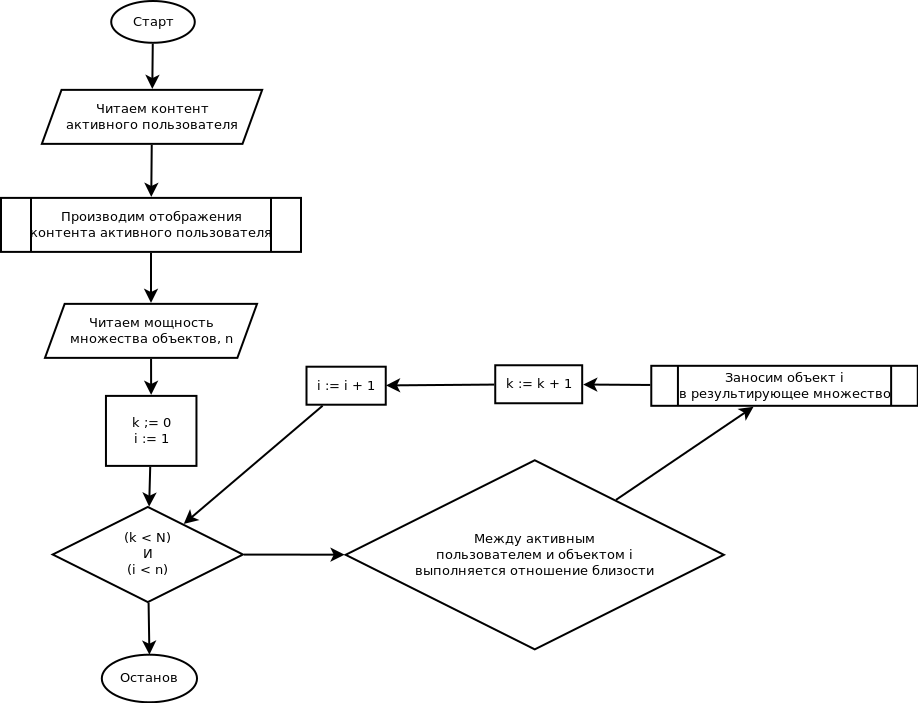
\includegraphics[width=7in,height=8in]{pics/algs/fuz-topn.png}
\end{center}
\end{figure}
Блок-схеме (\ref{dia:fuz-topn}) соответствует псевдокод, представленный на
изображении <<Алгоритм решения задачи $topN$ при использовании правила
	вывода нечеткой модели>> (\ref{alg:fuz-topn}).

\begin{figure}[htb]
	\caption{Алгоритм решения задачи $topN$ при использовании правила
	вывода нечеткой модели}
	\label{alg:fuz-topn}
	%\begin{algorithm}
		\begin{algorithmic}[1]
			\State $n \gets 1$
			\State $I_{topN} \gets \varnothing$
			\For {$i \gets 1 \to |I|$}
			\If{$\rh(u_a, i) \ge \Delta_{\R}$}
			\State $I_{topN} \gets I_{topN} \bigcup \{ i \}$
			\State $n \gets n + 1$
			\EndIf
			\If{$n = N$}
			\State Стоп
			\EndIf
			\EndFor
		\end{algorithmic}
	%\end{algorithm}
\end{figure}

\subsection{Свойства решения задачи $topN$}
\begin{trm}
	\label{pif_acc}
	Если $\Pi_f$ определено разработчиками так, что $\forall$ $(u_a, i, \rho(u_a, i)) \in P$
	$|\rho(u_a, i) - \rh(u_a, i)| = 0$, то эффективность решения
	по критерию качества гарантированна.
\end{trm}

Результирующее множество имеет вид $\{(u_a, i, \rh(u_a, i)): \rh(u_a, i) \ge
\Delta_{\R}\}$. Так как $|\rho(u_a, i) - \rh(u_a, i)| = 0$, поэтому
$\rh(u_a, i) \ge \Delta_{\R}$, а, значит, $u_a \R i$ и решение эффективно по
$\eat$, что и требуется по задаче.

Таким образом, получаем, что
\begin{trm}
	\label{fuz-cond-topn}
достаточным условием эффективности решения задачи $topN$ по критерию качества является
такое задание $\Pi_f$, что
$|\rh(u_a, i) - \rho(u_a, i)| = 0$
\end{trm}

Асимптотическая сложность решения задачи $topN$ равна $O(|I|)$.

\subsection{Решение задачи прогнозирования}
Правило вывода нечеткой модели (\ref{my-pi}) заключается в реализации функции $\rh$.
Поэтому прямое решение задачи прогнозирования, без применения каких-либо
алгоритмов, заключается только в расчете значения $\rh(u_a, i_{\bot})$.


На рисунке <<Блок-схема алгоритма решения задачи прогнозирования в нечеткой модели при
	использовании $\Pi_f$>> (\ref{dia:fuz-p}) изображена блок-схема алгоритма
решения задачи прогнозирования  в нечеткой модели при использовании
правила вывода $\Pi_f$.
\begin{figure}[hbtp]
	\caption{Блок-схема алгоритма решения задачи прогнозирования в нечеткой модели при
	использовании $\Pi_f$}
\begin{center}
	\label{dia:fuz-p}
 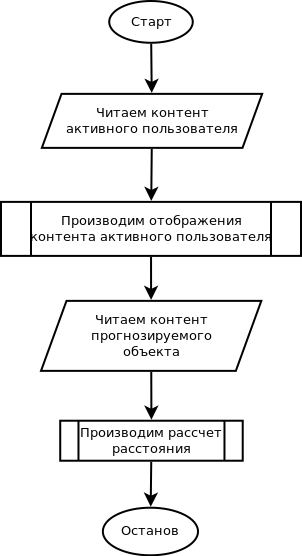
\includegraphics[width=4in,height=5in]{pics/algs/fuz-p.png}
\end{center}
\end{figure}
Блок-схеме (\ref{dia:fuz-p}) соответствует псевдокод, представленный на
изображении <<Алгоритм решения задачи прогнозирования при использовании правила
	вывода нечеткой модели>> (\ref{alg:fuz-p}).

\begin{figure}[htb]
	\caption{Алгоритм решения задачи прогнозирования при использовании правила
	вывода нечеткой модели}
	\label{alg:fuz-p}
	%\begin{algorithm}
		\begin{algorithmic}[1]
			\State $\rh(u_a, i_{\bot})$ \Comment{Нужно провести только расчет
			прогнозной функции}
		\end{algorithmic}
	%\end{algorithm}
\end{figure}

%\begin{figure}[h]
%\caption{Решение задачи прогнозирования}
%\begin{algorithm}\label{mysolve-p}
%\begin{algorithmic}[1]
%\State $\delta(u_a, i_{\bot}) \gets 1 - \rh(u_a, i_{\bot})$
%\end{algorithmic}
%\end{algorithm}
%\end{figure}

\subsection{Свойства решения задачи прогнозирования}

\begin{trm}
	\label{pif_acc_pred}
	Если $\Pi_f$ определено разработчиками так, что $\forall$ $(u_a, i, \rho(u_a, i)) \in P$
	$|\rho(u_a, i) - \rh(u_a, i)| \le \varepsilon_p$, то эффективность решения
	по критерию качества гарантированна.
\end{trm}

Эффективность решения задачи $pred$ зависит от
аккуратности задания $\Pi_f$.
Если функция $\rh$ реализована так, что
$|\rh(u_a, i) - \rho(u_a, i)| \le \varepsilon_p$, то решение будет эффективным,
что следует из способа решения задачи.

Таким образом, получаем, что
\begin{trm}
	\label{fuz-cond-pred}
достаточным условием эффективности решений по критерию качества является
такое задание $\Pi_f$, что
$|\rh(u_a, i) - \rho(u_a, i)| \le \varepsilon_p$
\end{trm}

Асимптотическая сложность решения задачи $pred$ равна $O(C)$.
%\subsection{Интерполяционное решение задачи прогнозирования}
%
%\subsection{Свойства интерполяционного решения задачи прогнозирования}




	        % Введение

\section{Сравнение коллаборативной и нечеткой моделей рекомендательной системы}
Сравним эффективность моделей по критериям качества решения, вычислительной
сложности и стабильности.
%При реализации нечеткой модели разработчик
%единожды создает программный код самой модели. Если нужно что-то изменить,
%то меняется стратегия, которая заключается в задании функции $\delta_c$, но не код.
\subsection{Эффективность по критерию качества}
\begin{trm}
	\label{trm:fuz-eff-extension}
	Нечеткая модель является эффективным по критерию качества расширением АКМ.
\end{trm}
Нечеткая модель включает в себя АКМ по применяемым правилам вывода.
При этом коллаборативные правила вывода в нечеткой модели дают большую
эффективность, чем применение тех же правил в АКМ, так как в нечеткой
модели выполняются условия получения эффективного решения по критерию качества
при применении коллаборативных правил вывода, что было показано в разделе
<<Применение коллаборативных правил вывода в нечеткой модели>>.

Эффективность нечеткой модели по критерию качества при применении правила
вывода $\Pi_f$ так же, как и в коллаборативных моделях ограничена
дополнительным условием. Для нечеткой модели и $\Pi_f$ --- это требования
к заданию $\Pi_f$, которые выражены достаточными условиями
(\ref{fuz-cond-pred}) и (\ref{fuz-cond-topn}). Как и в АКМ выполнение этого условия
зависит от разработчиков системы. Однако в АКМ разработчик
обладает меньше свободой действий, чем в нечеткой модели. Все, что доступно
разработчику в АКМ --- это выбор функции, которая будет
использоваться в качестве меры сходства, и ее порогового значения. В нечеткой
модели разработчик выбирает алгоритмы, эвристики, наборы данных, знания и т.п.,
чтобы задать правила вывода. При этом было показано, что если правило вывода
$\Pi_f$ задано так, что выполняются (\ref{fuz-cond-pred}) и
(\ref{fuz-cond-topn}), то решение будет гарантированно эффективно.
Для АКМ такую гарантию дать нельзя, так как существует зависимость от исходных
данных. Поэтому теоретически нечеткая модель более
эффективна, чем АКМ, и является ее расширением, так как включает
в себя коллаборативные правила вывода, и может применяться на любых данных
о пользователе $X$ и объекте, а не только тога, когда $X = I$ И $Y = X$.

Правила вывода РС задают взаимосвязь между информацией о пользователе и об
объекте. В правилах вывода
АКМ эта взаимосвязь заложена статически в качестве эвристик, выполнение
которых не гарантировано. Для нечеткой модели взаимосвязь является
динамической. Ее можно рассматривать как паттерн программирования
<<стратегия>>. При реализации нечеткой модели разработчик
единожды создает программный код самой модели. Если нужно что-то изменить,
то меняется стратегия, но не код.

\subsection{Эффективность по критерию стабильности}
\begin{trm}
	\label{trm:fuz-eff-extension-stab}
	Нечеткая модель является эффективным расширением АКМ
	по критерию стабильности.
\end{trm}

Эффективность по качеству решений, получаемых в АКМ зависит от свойств исходных
данных, поэтому АКМ неэффективны по критерию стабильности. В том числе, если
мощность $P$ мала или вовсе равна нулю, то АКМ даже нельзя применять для
решения.

При применении
правила вывода $\Pi_f$ в нечеткой модели эффективность по качеству решения
не зависит от свойств исходных данных, зависит только от разработчика.

\subsection{Эффективность по критерию вычислительной сложности}
  \begin{table}[h]
	  \begin{center}
		  \caption{Асимптотические сложности алгоритмов решений}
		  \label{ass-comp}
		  \begin{tabular}{|c|c|c|c|}
			  \hline
			  Модель   & Правило вывода & Задача & Сложность  \\ \hline
			  ООМ      & $\Pi_{O}$ & $topN$ & $O(n^2)$  \\ \hline
			  СОМ      & $\Pi_{C}$ &Прогнозирование & $O(m)$ \\ \hline
			  Нечеткая & $\Pi_{O}$ &$topN$ & $O(n^2)$  \\ \hline
			  Нечеткая & $\Pi_{C}$ &Прогнозирование & $O(m)$ \\ \hline
			  Нечеткая & $\Pi_{f}$ &$topN$ & $O(n)$  \\ \hline
			  Нечеткая & $\Pi_{f}$ &Прогнозирование & $O(C)$ \\ \hline
		  \end{tabular}
	  \end{center}
  \end{table}

\begin{assert}
	\label{ass:eff-calc}
	Нечеткая модель является эффективным расширением АКМ
	по критерию вычислительной сложности.
\end{assert}

\subsection{Выводы}
В ходе диссертационного исследования была разработана
математическая модель РС, которая является эффективным
расширением АКМ по всем заданным критериям.
%\begin{enumerate}
%	\item Зависимость от свойств исходных данных: динамики, неоднородности,
%		мощности. Решения в нечеткой контентной модели в общем случае не
%		зависят от свойств исходных данных. Если мощность исходных данных мала,
%		то АКМ не применимы для решения задач. Если исходные данные обладают
%		свойством динамики или неоднородности, то АКМ не гарантируют получения
%		качественного решения.
%
%	\item Асимптотическая сложность. Алгоритмы решений задач нечеткой контентной модели
%		обладают асимптотической сложность, меньшей на порядок асимптотических
%		сложностей
%		алгоритмов решений АКМ;
%
%	\item Качество решений. Качество решений в контентной нечеткой модели
%		зависит от разработчика --- от аккуратности задания $\delta_c$.
%		Если функция задана аккуратно, то решения качественны.
%
%		Качество решений в АКМ зависят от разработчика --- от выбора
%		$\du, \di$ и $\Delta_u, \Delta_i$. Если эти параметры выбраны так, что
%		выполняются достаточные условия, то АКМ не гарантирует получение
%		качественных решений, так как это зависит в том числе и от свойств
%		исходных данных.
%\end{enumerate}
	        % Введение


           % Глава 3
\chapter{ТЕСТИРОВАНИЕ МОДЕЛЕЙ}
В данном разделе опишем разработанное программное обеспечение, с помощью
которого было проведено тестирование, данные, на которых проводилось
тестирование, а также представим и проанализируем полученные результаты.
\section{Описание программного обеспечения}
Программное обеспечение было написано на языке программирования
C++ по стандарту C++-11 под ОС Ubuntu. Сборка проекта осуществлялась
с помощью Cmake, использовался компилятор GNU.

Программное обеспечение работает с исходными данными,
данными о пользователях и объектах, которые хранятся в базе данных.
Пользователь исходного кода может сделать некоторые дополнения и
использовать другую базу данных. Класс подключения к базе создается
с помощью фабрики объектов.
Базовым классом, представляющим эту фабрику, является класс
ConnectionFactory, который имеет чистый виртуальный (pure virtual)
метод create и описан в файле db/connection-pool/ConntectionPool.h.
Пользователь должен сформировать собственную фабрику, класс которой
будет являться дочерним классом класса ConnectionFactory и которая
будет создавать объекты-коннекторы к конкретной базе.
Фабрика объектов-коннекторов создает объекты типа
std::shared\_ptr<Connection>, для которого определены чистые виртуальные методы
query и exec.
В разработанном
программном обеспечении данные хранились в базе MySql, поэтому был
создан класс MySQLConnectionFactory, в параметры конструктора которого
передаются параметры подключения к базе: хост, имя базы, логин и
пароль. В этом классе перегружен метод create, в теле которого
создается новое подключение к базе данных MySql, используя те
параметры, что были переданы в конструктор класса
MySQLConnectionFactory. Подключение происходит с помощью библиотеки
cppconn. Фабрика MySQLConnectionFactory создает объекты-коннекторы
типа MySQLConnection, в котором определены методы exec и query.
Таким образом, пользователь должен объявить два класса:
наследника класса ConnectionFactory и наследника класса Connection.
Фабрика, с помощью которой будет осуществляться создание объектов-коннекторов
и тип объектов коннекторов являются шаблонными параметрами класса
DbPoolGeneral, описанного в файле db/dbPool.h. Пользователю нужно
лишь указать имена этих параметров в определении typedef в конце файла,
как это сделано в текущем проекте:
\begin{verbatim}
	typedef DbPoolGeneral<
		active911::MySQLConnection,
		active911::MySQLConnectionFactory>

		DbPool;
\end{verbatim}
При использовании других баз и коннекторов нужно также внести изменения в файл
db/CmakeLists.txt и указать, какие библиотеки используются.

Интерфейсом пользователя программного обеспечения является командная
строка, в которой пользователь указывает параметры запуска.
Параметры запуска программы делятся на несколько логических групп,
а каждой группе принадлежит некоторое множество параметров:

\begin{itemize}
	\item параметры модели:
	\begin{itemize}
		\item $sim$ --- выбор функции, которая будет использоваться в качестве
			меры сходства. Реализованы следующие функции и соответствующие им
			имена параметров:
			\begin{itemize}
				\item $cos$ --- косинус угла между контами-векторами;
				\item $pearson$ --- коэффициент корреляции Пирсона;
				\item $hamming$ --- обобщенное расстояние Хэмминга.
			\end{itemize}
		\item $uidelta$ --- пороговое значение, которое соответствует
			$\Delta_{\R}$
		\item $delta$ --- пороговое значение меры сходства, соответствует
			$\Delta_u$ или $\Delta_i$.
	\end{itemize}
	\item параметры задачи:
	\begin{itemize}
		\item $N$ --- число объектов при решении задачи $topN$;
		\item $task$ --- решаемая задача. Либо параметр равен $p$, либо $topn$;
		\item $neighn$ --- число соседей, которые войдут в кластер;
		\item $sltn$ --- способ решения задачи. Реализованы следующие способы
			решения, которые может выбрать пользователь:
			\begin{itemize}
				\item $std$ --- стандартное решение задач методами коллаборативной
					фильтрации;
				\item $linear$ --- решение задачи $topN$ линейным поиском в нечеткой
					модели;
				\item $rnd$ --- случайное решение;
				\item $direct$ --- прямое вычисление $\rho(u_a, i)$, то есть
					решение задачи прогнозирования в нечеткой модели.
			\end{itemize}
	\end{itemize}
	\item функциональные параметры:
		\begin{itemize}
			\item $resplit$ --- опциональный параметр.опциональный параметр.
				Если он указан в командной строке, тогда произойдет разбиение
				исходных данных на обучающее и тестовое множество;
			\item $eval$ --- если параметр указан, то произойдет оценка
				качества и результаты сохранятся в соответствующей базе;
			\item $split\_alg$ --- алгоритм разбиения исходных данных на
				обучающее и тестовое множество. Возможны следующие варианты:
				\begin{itemize}
					\item $std$ --- стандартное разбиение, которое производится
						в случайном порядке;
					\item $div$ --- от diverse. Алгоритм формирует данные для
						каждого пользователя так,
						что в обучающем множестве находятся такие объекты между
						которыми и объектами тестового множества не выполняется
						отношение близости, если это возможно.
				\end{itemize}
			\item $split\_pcnt$ --- процент исходный данных, который войдет в
				обучающее множество;
			\item $calc$ --- если параметр указан, то будет произведено решение
				задачи --- если параметр указан, то будет произведено решение
				задачи;;
			\item $truncate$ --- очищение базы данных. Можно очистить один из
				четырех типов баз:
				\begin{itemize}
					\item $train$ --- обучающие данные;
					\item $test$ --- тестовые данные;
					\item $eval$ --- результаты оценки качества;
					\item $rslt$ --- результирующее множество.
				\end{itemize}
				Конкретное же имя базы формируется так:
				\begin{itemize}
					\item type + postfix, где type $\in \{eval, rslt\}$, postfix
						=
					$task$ + \_ + $sltn$ + \_ + $sim$ + \_ + $uidelta$ + \_ $delta$ +
					\_ $split$ + \_ + $split\_pcnt$ + $neighn$, где $task$ и
						т.д. конкретные значения указанных параметров, а знак +
						означает конкатеннацию строк;
					\item type + \_ + $task$ + \_ + $split\_pcnt$ +
						$split\_alg$,
						где type $\in \{train, test\}$, $task$ и т.п.
						означает конкретное значение соответствующего типа, указанного в
						командной строке.
				\end{itemize}

		\end{itemize}
\end{itemize}

Таким образом, пользователь с помощью командной строки
может запустить программу на выполнение следующих задач:
решить задачу при использовании различных параметров,
очистить базу данных, произвести расчет
оценки качества и разбить исходное множество на тестовое и обучающее.

Приведем несколько основных примеров запусков программы.

\begin{figure}[H]
	\caption{Пример запуска решения задачи $topN$ в ООМ}
	\label{pic:ex-topn-cos}
	\begin{center}
  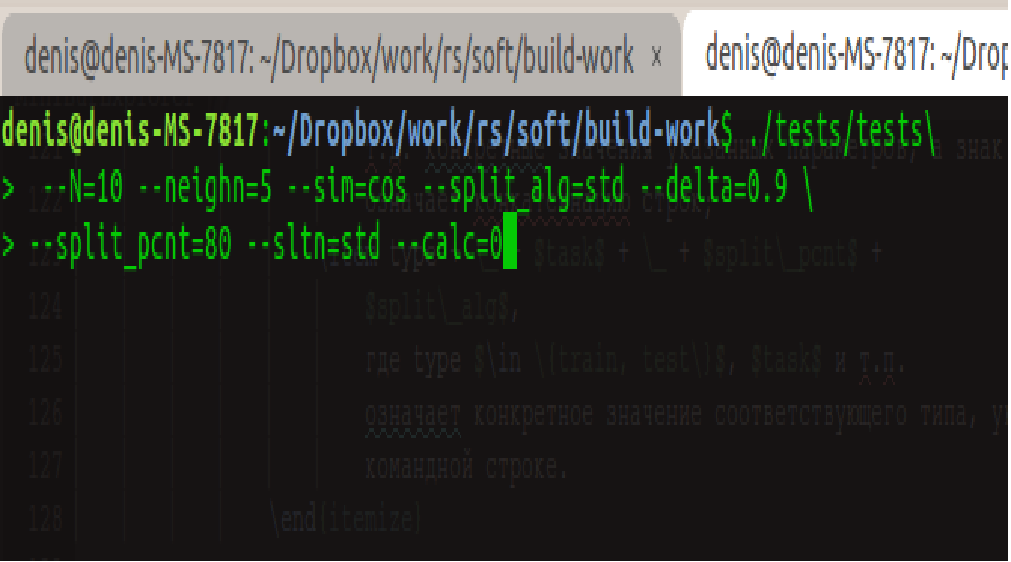
\includegraphics[width=7in,height=3in]{pics/examples/topn-cos.png}
\end{center}
\end{figure}

Пример запуска решения задачи $topN$ в ООМ стандартным
алгоритмом (\ref{alg:topn-solve-ors}) со следующими параметрами
\begin{itemize}
	\item $N=10$;
	\item мера сходства --- косинус;
	\item $\Delta_i = 0,9$;
	\item стандартное разбиение исходного множества данных на обучающее и
		тестовое множество;
	\item в обучающее множество входит 80\% исходных данных;
\end{itemize}
представлен на рисунке <<Пример запуска решения задачи $topN$ в ООМ>> (\ref{pic:ex-topn-cos}).

Пример запуска решения задачи $topN$ в нечеткой модели стандартным
алгоритмом (\ref{alg:topn-solve-ors}) со следующими параметрами:
\begin{itemize}
	\item $N=10$;
	\item $\Delta_i = 0,1$;
	\item стандартное разбиение исходного множества данных на обучающее и
		тестовое множество;
	\item в обучающее множество входит 80\% исходных данных;
\end{itemize}
представлен на рисунке <<Пример запуска решения задачи $topN$ в нечеткой модели при
	использовании $\Pi_C$>> (\ref{pic:ex-topn-hamming}).

\begin{figure}[H]
	\caption{Пример запуска решения задачи $topN$ в нечеткой модели при
	использовании $\Pi_C$}
	\label{pic:ex-topn-hamming}
	\begin{center}
  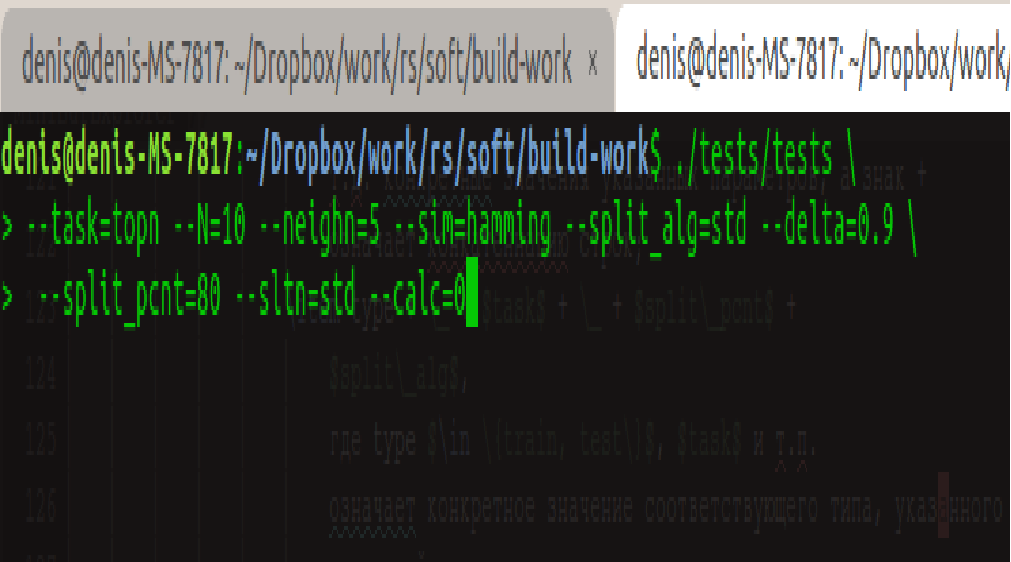
\includegraphics[width=7in,height=3in]{pics/examples/topn-hamming.png}
\end{center}
\end{figure}

Пример запуска решения задачи $topN$ в нечеткой модели
при использовании алгоритма линейного поиска (\ref{alg:fuz-topn}) со следующими
параметрами:
\begin{itemize}
	\item $N=10$;
	\item $\varepsilon_{\R} = 0,9$;
	\item стандартное разбиение исходного множества данных на обучающее и
		тестовое множество;
	\item в обучающее множество входит 80\% исходных данных;
\end{itemize}
представлен на рисунке <<Пример запуска решения задачи $topN$ в нечеткой модели при
	использовании $\Pi_f$>> (\ref{pic:ex-topn-fuz}).

\begin{figure}[H]
	\caption{Пример запуска решения задачи $topN$ в нечеткой модели при
	использовании $\Pi_f$}
	\label{pic:ex-topn-fuz}
	\begin{center}
	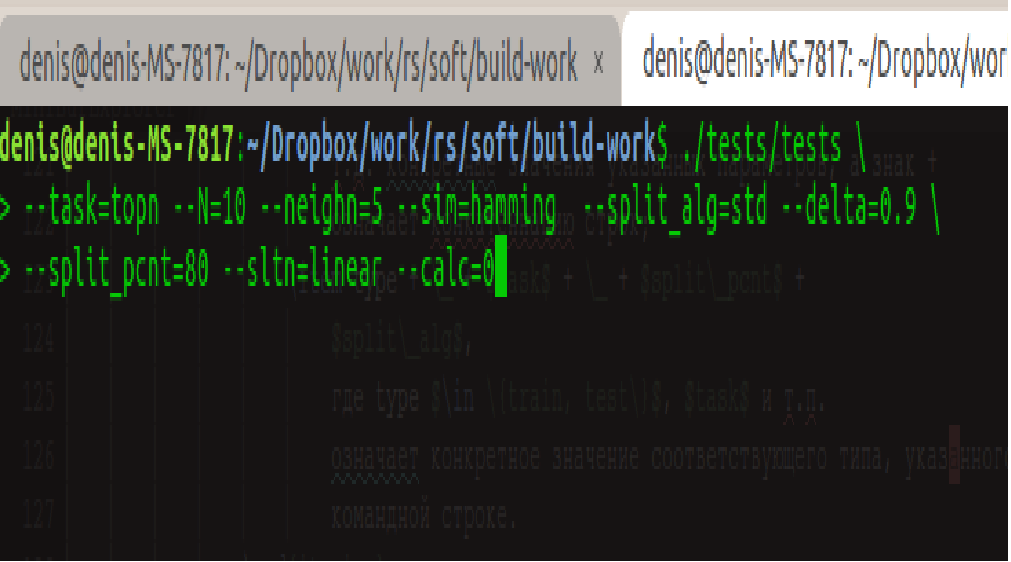
\includegraphics[width=7in,height=3in]{pics/examples/topn-fuz.png}
\end{center}
\end{figure}
%%%%%%%%%%%%%%%%%%%%%%%% p
Пример запуска решения задачи прогнозирования в CОМ стандартным
алгоритмом (\ref{alg:p-srs}) со следующими параметрами
\begin{itemize}
	\item мера сходства --- коэффициент корреляции Пирсона;
	\item $\Delta_u = 0,9$;
	\item стандартное разбиение исходного множества данных на обучающее и
		тестовое множество;
	\item в обучающее множество входит 80\% исходных данных;
\end{itemize}
представлен на рисунке <<Пример запуска решения задачи прогнозирования в СОМ>> (\ref{pic:ex-p-srs}).

\begin{figure}[H]
	\caption{Пример запуска решения задачи прогнозирования в СОМ}
	\label{pic:ex-p-srs}
	\begin{center}
  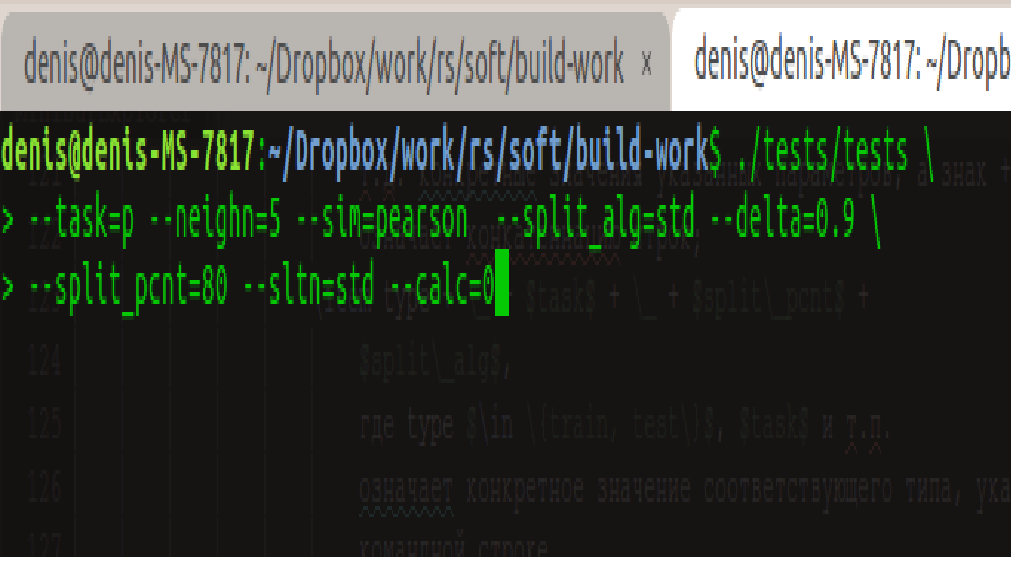
\includegraphics[width=7in,height=3in]{pics/examples/p-pearson.png}
\end{center}
\end{figure}

Пример запуска решения задачи прогнозирования в нечеткой модели стандартным
алгоритмом (\ref{alg:p-srs}) со следующими параметрами:
\begin{itemize}
	\item $\Delta_u = 0,1$;
	\item в обучающее множество входит 80\% исходных данных;
\end{itemize}
\begin{figure}[H]
	\caption{Пример запуска решения задачи прогнозирования в нечеткой модели при
	использовании $\Pi_C$}
	\label{pic:ex-p-srs-hamming}
	\begin{center}
  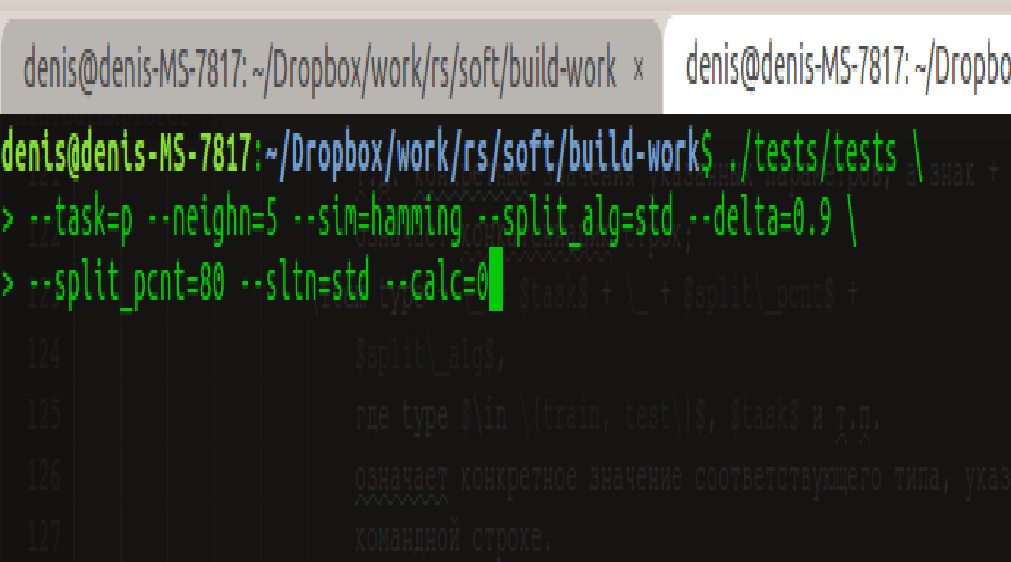
\includegraphics[width=7in,height=3in]{pics/examples/p-hamming.png}
\end{center}
\end{figure}
представлен на рисунке <<Пример запуска решения задачи прогнозирования в нечеткой модели при
	использовании $\Pi_C$>> (\ref{pic:ex-p-srs-hamming}).

Пример запуска решения задачи прогнозирования в нечеткой модели
алгоритмом нечеткой модели (\ref{alg:fuz-p}) со следующими параметрами:
\begin{itemize}
	\item $\varepsilon_{\R} = 0,9$;
	\item стандартное разбиение исходного множества данных на обучающее и
		тестовое множество;
	\item в обучающее множество входит 80\% исходных данных;
\end{itemize}
\begin{figure}[H]
	\caption{Пример запуска решения задачи прогнозирования в нечеткой модели при
	использовании $\Pi_f$}
	\label{pic:ex-p-srs-fuz}
	\begin{center}
  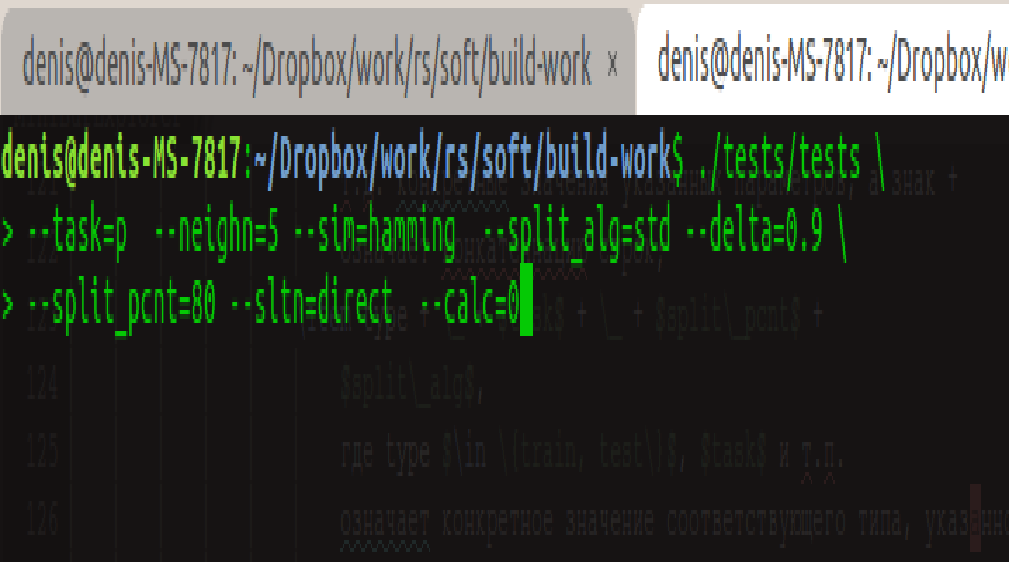
\includegraphics[width=7in,height=3in]{pics/examples/p-fuz.png}
\end{center}
\end{figure}
представлен на рисунке <<Пример запуска решения задачи прогнозирования в нечеткой модели при
	использовании $\Pi_f$>> (\ref{pic:ex-p-srs-hamming}).

%%%%%%%%%%%%%%%%%%%%
Пример очистки таблиц, в которых находятся результаты решения и оценки качества
решения задачи $topN$ в нечеткой модели представлен на рисунке <<Пример очистки
таблицы результатов и таблицы со значениями оценок качества>>.
(\ref{pic:truncate}).
\begin{figure}[H]
	\caption{Пример очистки таблицы результатов и таблицы со значениями оценок качества}
	\label{pic:truncate}
	\begin{center}
  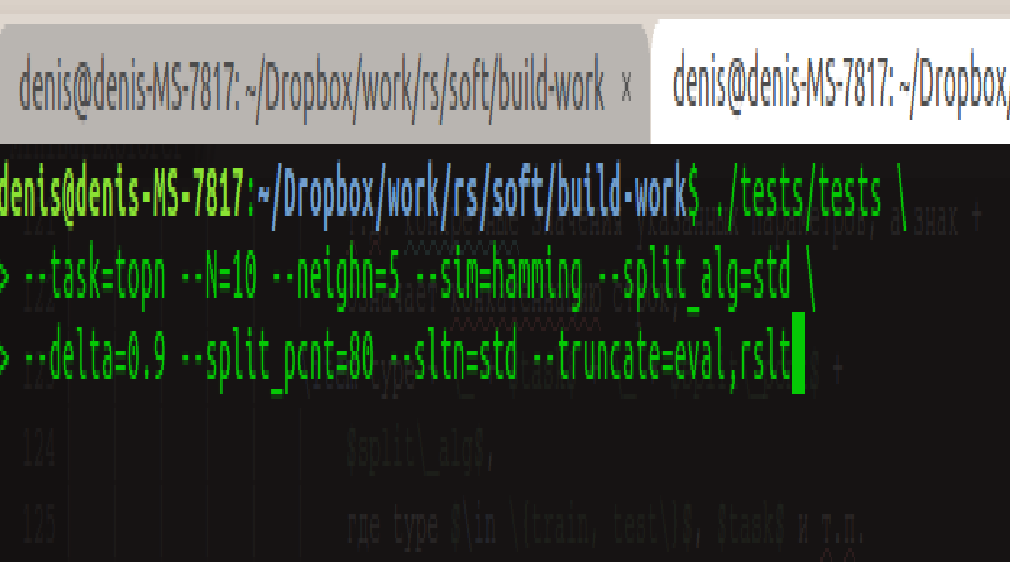
\includegraphics[width=7in,height=3in]{pics/examples/truncate.png}
\end{center}
\end{figure}

Пример вывода значений $P, AveP, NDCG$ при решении задачи $topN$ в нечеткой
модели при применении $\Pi_O$ представлен на рисунке <<Пример запуска программного обеспечения для вывода средних значений оценок
качества>> (\ref{pic:eval}).
\begin{figure}[H]
	\caption{Пример запуска программного обеспечения для вывода средних значений оценок
качества}
\label{pic:eval}
	\begin{center}
  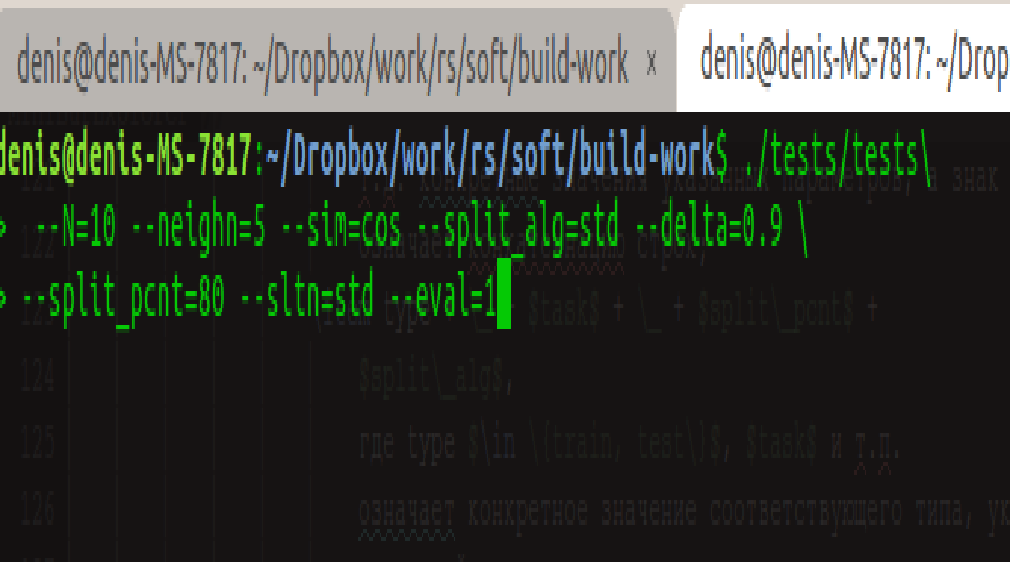
\includegraphics[width=7in,height=3in]{pics/examples/eval.png}
\end{center}
\end{figure}

Пример разбиения множества исходных данных на обучающее множество и тестовое
при применении стандартного алгоритма в пропорции 80 к 20 соответственно
представлен на рисунке <<Пример запуска программного обеспечения для формирования обучающего и тестового
множества при использовании разбиения 80 к 20 случайным образом (стандартное
разбиение)>> (\ref{pic:resplit}).
\begin{figure}[H]
	\caption{Пример запуска программного обеспечения для формирования обучающего и тестового
множества при использовании разбиения 80 к 20 случайным образом (стандартное
разбиение)}
\label{pic:resplit}
	\begin{center}
  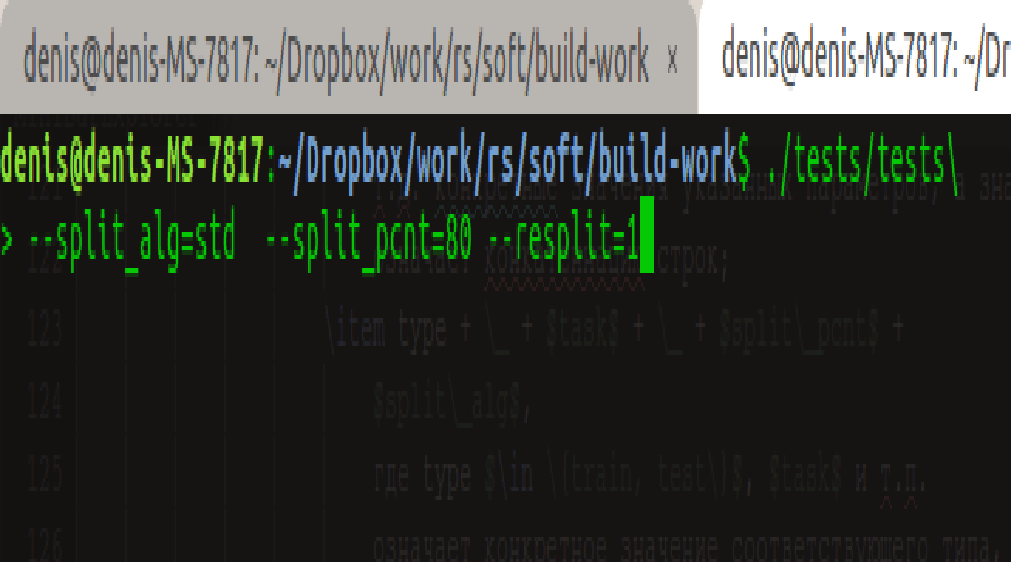
\includegraphics[width=7in,height=3in]{pics/examples/resplit.png}
\end{center}
\end{figure}

%\section{Описание входных данных}
Для того, чтобы провести практическое сравнение по критериям эффективности
было проведено тестирование на реальных исходных данных с помощью программного
обеспечения, описанного в предыдущем разделе. Опишем данные, на которых
проводилось тестирование.

Тестирования проводились на новейшем сформированном
множестве данных MovieLens \cite{ml-data}.
Эти исходные данные были собраны компанией MovieLens, которая
занимается исследованиями и разработками в области РС. Исходные
данные не являются синтетическими данными, а данными,
которые были заполнены реальными
пользователями. Множество данных MovieLens характеризуется следующими
показателями:
\begin{itemize}
	\item $|U| = 700$;
	\item $|I| = 9000$ --- объектами являются фильмы;
	\item $|P| = 100000$;
	\item $|Y| = 18$ --- характеристикой фильма является кинематографический
		жанр.
\end{itemize}
Список жанров-характеристик объектов:
\begin{itemize}
	\item action;
	\item adventure;
	\item animation;
	\item children's;
	\item comedy;
	\item crime;
	\item documentary;
	\item drama;
	\item fantasy;
	\item film-Noir;
	\item horror;
	\item musical;
	\item mystery;
	\item romance;
	\item sci-Fi;
	\item thriller;
	\item war;
	\item western.
\end{itemize}

Для АКМ $X = I$ и $w_U(u, x) = \rho(u,x), x \in I$.

Для задания правила вывода $\Pi_f$ была аналитически определена
функция $\delta_c$, основываясь на эвристическом предположении о том,
что между оценкой близости $\rho(u, i)$, заданной пользователем $u$
и характеристикой $y \in Y$ объекта $i$,
то есть жанром фильма, существует корреляция:
\begin{multline}
	\delta_c(i, y) = \frac{1}{|\{i: \exists \rho(u,i)\}|}
	\cdot
	|\{ i : (\rho(u, i) < \varepsilon_1) \wedge (\nu(y) = 1)\}| -\\
	|\{ i : (\rho(u, i) > \varepsilon_2) \wedge (\nu(y) = 1)\}|, \\
	\text{ где }
	\varepsilon_1 = 0,2, \varepsilon_2 = 0,6;
\end{multline}

Такое эвристическое предположение верно не для всех пользователей, так как
их вкусы могут быть неоднородными. Поэтому для некоторых пользователей функция
$\delta_c$ задана так, что
$|\rh(u, i_{\bot}) - \rho(u, i_{\bot}) \le \varepsilon_p|$,
а для некоторых --- нет.

\section{Сравнение моделей по критерию качества решений}

\subsection{Задача $topN$}

Результаты представляются графиком и таблицей для каждого пункта.
Координатой оси $X$ является идентификатор пользователя, координатой
оси $Y$ является значение оценки качества.
В качестве функции $\eit$ использовалась функция
<<точность>> (P) \ref{precision}.
Другие функции рассматривались так же, но между
функциями одного класса существует корреляция и приведение других графиков
оказывается избыточным.

На графиках представляются данные по двум методам тестирования. Для наглядности
результирующие данные были отсортированы по значениям оценки качества,
принадлежащим первому методу (в каждой паре точек, которые находятся на одной
вертикали, идентификаторы пользователей совпадают).

В таблицах представлены средние значения оценок точности по всем пользователям.


Для проведения тестов данного пункта исходные данные были
стандартно разбиты на тестовое и обучающее множество по следующему принципу:
разбиение проводилось случайно, в обучающее множество входит
80\% данных, в тестовое --- оставшиеся 20\%. В тестировании участвовало
подмножество $P^{\prime} \subset P, P^{\prime} = \{(u, i, \rho(u, i)):
\rho(u, i) = 1\}$.

\subsubsection{Влияние свойства транзитивности на ООМ при решении задачи $topN$}
В данном пункте приведем и сравним результаты решения задачи $topN$, полученные:
\begin{enumerate}
	\item  в ООМ при следующих параметрах:
		\begin{itemize}
			\item
			стандартный алгоритма решения задачи
			$topN$ (\ref{alg:topn-solve-ors}), основанный на
			правиле вывода $\Pi_O$;
			\item
			пороговое значение $\Delta_i$ равно $0,9$;
			\item
		применяемая мера сходства --- косинус угла (\ref{sim-cos})
		между контентами, которые представляются в ООМ в виде векторов.
		\end{itemize}
	\item  в ООМ при следующих параметрах:
		\begin{itemize}
			\item
			стандартный алгоритма решения задачи
			$topN$ (\ref{alg:topn-solve-ors}), основанный на
			правиле вывода $\Pi_O$;
			\item
			пороговое значение $\Delta_i$ равно $0,49$;
			\item
		применяемая мера сходства --- косинус угла (\ref{sim-cos})
		между контентами, которые представляются в ООМ в виде векторов.
		\end{itemize}
\end{enumerate}

При $\Delta_i = 0,9$ вероятность того, что $(i \rt j) \wedge (j \rt k)
\Rightarrow (i \rt k)$, выше, чем при $\Delta_i = 0,49$.
На Рис. \ref{pic:topn_trans} приведены результаты решений задачи $topN$ при
различных пороговых значениях. Черным цветом приведены результаты для
$\Delta_i = 0,9$, красным --- для $\Delta_i = 0,49$.
Видно, что при $\Delta_i = 0,9$ результаты решений эффективней, так
как большинство точек, соответствующих $\Delta_i = 0,9$ проходит ниже точек,
соответствующих $\Delta_i = 0,49$, что также подтверждается табличными данными,
представленными в таблице (\ref{tbl:topn_trans}).

Некоторые результаты при $\Delta_i = 0,9$ хуже, чем при
$\Delta_i = 0,49$. Это происходит для тех пользователей,
для которых характерно свойство неоднородности.

\begin{figure}[H]
	\caption{Влияние свойства транзитивности на ООМ при решении задачи $topN$}
	\label{pic:topn_trans}
	\begin{center}
		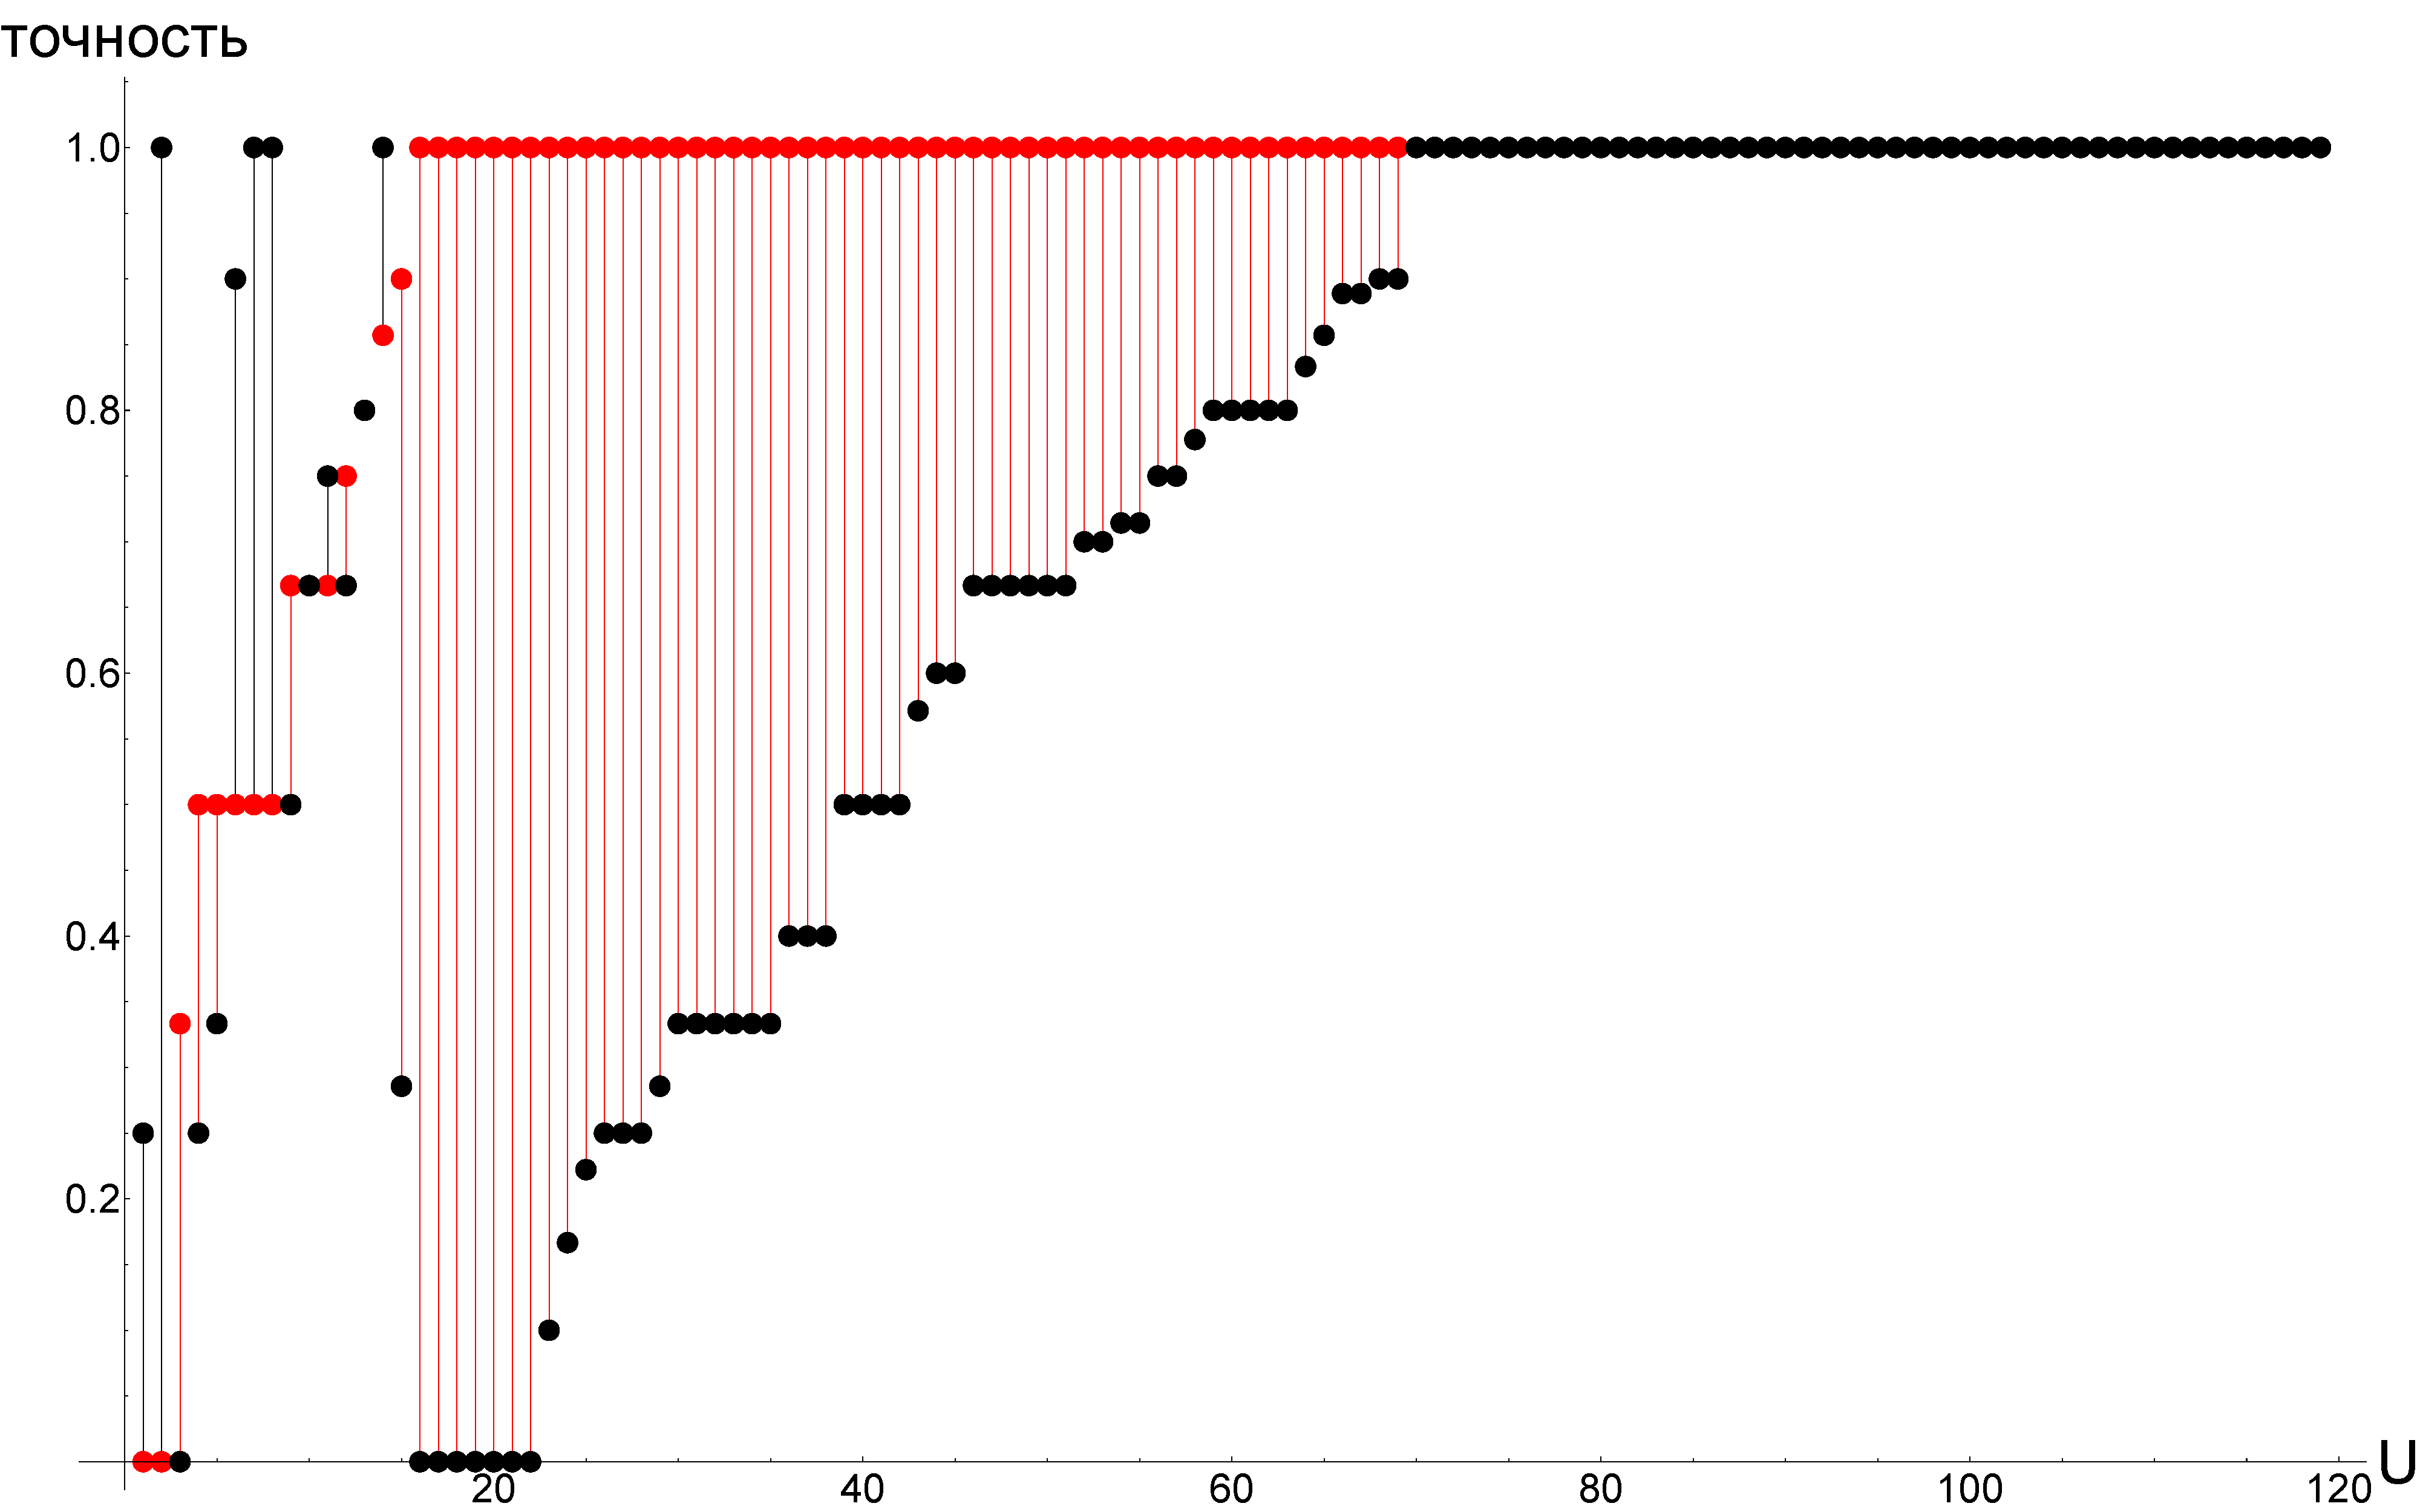
\includegraphics[width=7in,height=4in]{pics/results/transitivity.pdf}
\end{center}
\end{figure}

\begin{table}[H]
	\caption{Влияние свойства транзитивности на ООМ при решении задачи $topN$}
  \label{tbl:topn_trans}
  \begin{center}
	\begin{tabular}{|c|c|}
	  \hline
		Модель& Точность \\ \hline
		ООМ&0,925 \\ \hline
		Нечеткая&0,627 \\ \hline
	\end{tabular}
  \end{center}
\end{table}

\subsubsection{Применение правила вывода ООМ в коллаборативной и нечеткой
моделях}
В данном пункте приведем и сравним результаты решения задачи $topN$, полученные:
\begin{enumerate}
	\item  в ООМ при следующих параметрах:
		\begin{itemize}
			\item
			стандартный алгоритма решения задачи
			$topN$ (\ref{alg:topn-solve-ors}), основанный на
			правиле вывода $\Pi_O$;
			\item
			пороговое значение $\Delta_i$ равно $0,9$;
			\item
		применяемая мера сходства --- косинус угла (\ref{sim-cos})
		между контентами, которые представляются в ООМ в виде векторов.
		\end{itemize}
	\item в нечеткой при следующих параметрах:
		\begin{itemize}
			\item
			стандартный алгоритма решения задачи
			$topN$ (\ref{alg:topn-solve-ors}), основанный на
			правиле вывода $\Pi_O$;
			\item
				применяемая мера сходства --- обобщенное расстояние Хэмминга
				(\ref{fuz:rhi})
		\end{itemize}
\end{enumerate}

На Рис. \ref{pic:topn_pio} приведены результаты решения
задачи $topN$ при применении $\Pi_O$ в ООМ и нечеткой модели.
Черным цветом обозначены результаты решения в нечеткой модели.
Видно, что в большинстве случаев нечеткая модель более эффективна
по критерию качества. В обратных ситуациях предпочтения пользователя
неоднородны.
%, и $\delta_c$ для таких пользователей определена так, что
%$|\rho(u, i) - \rh(u, i)| > \varepsilon_p$.

\begin{figure}[H]
	\caption{Качество решений при применении правила вывода $\Pi_{O}$ в нечеткой модели и ООМ}
	\label{pic:topn_pio}
	\begin{center}
		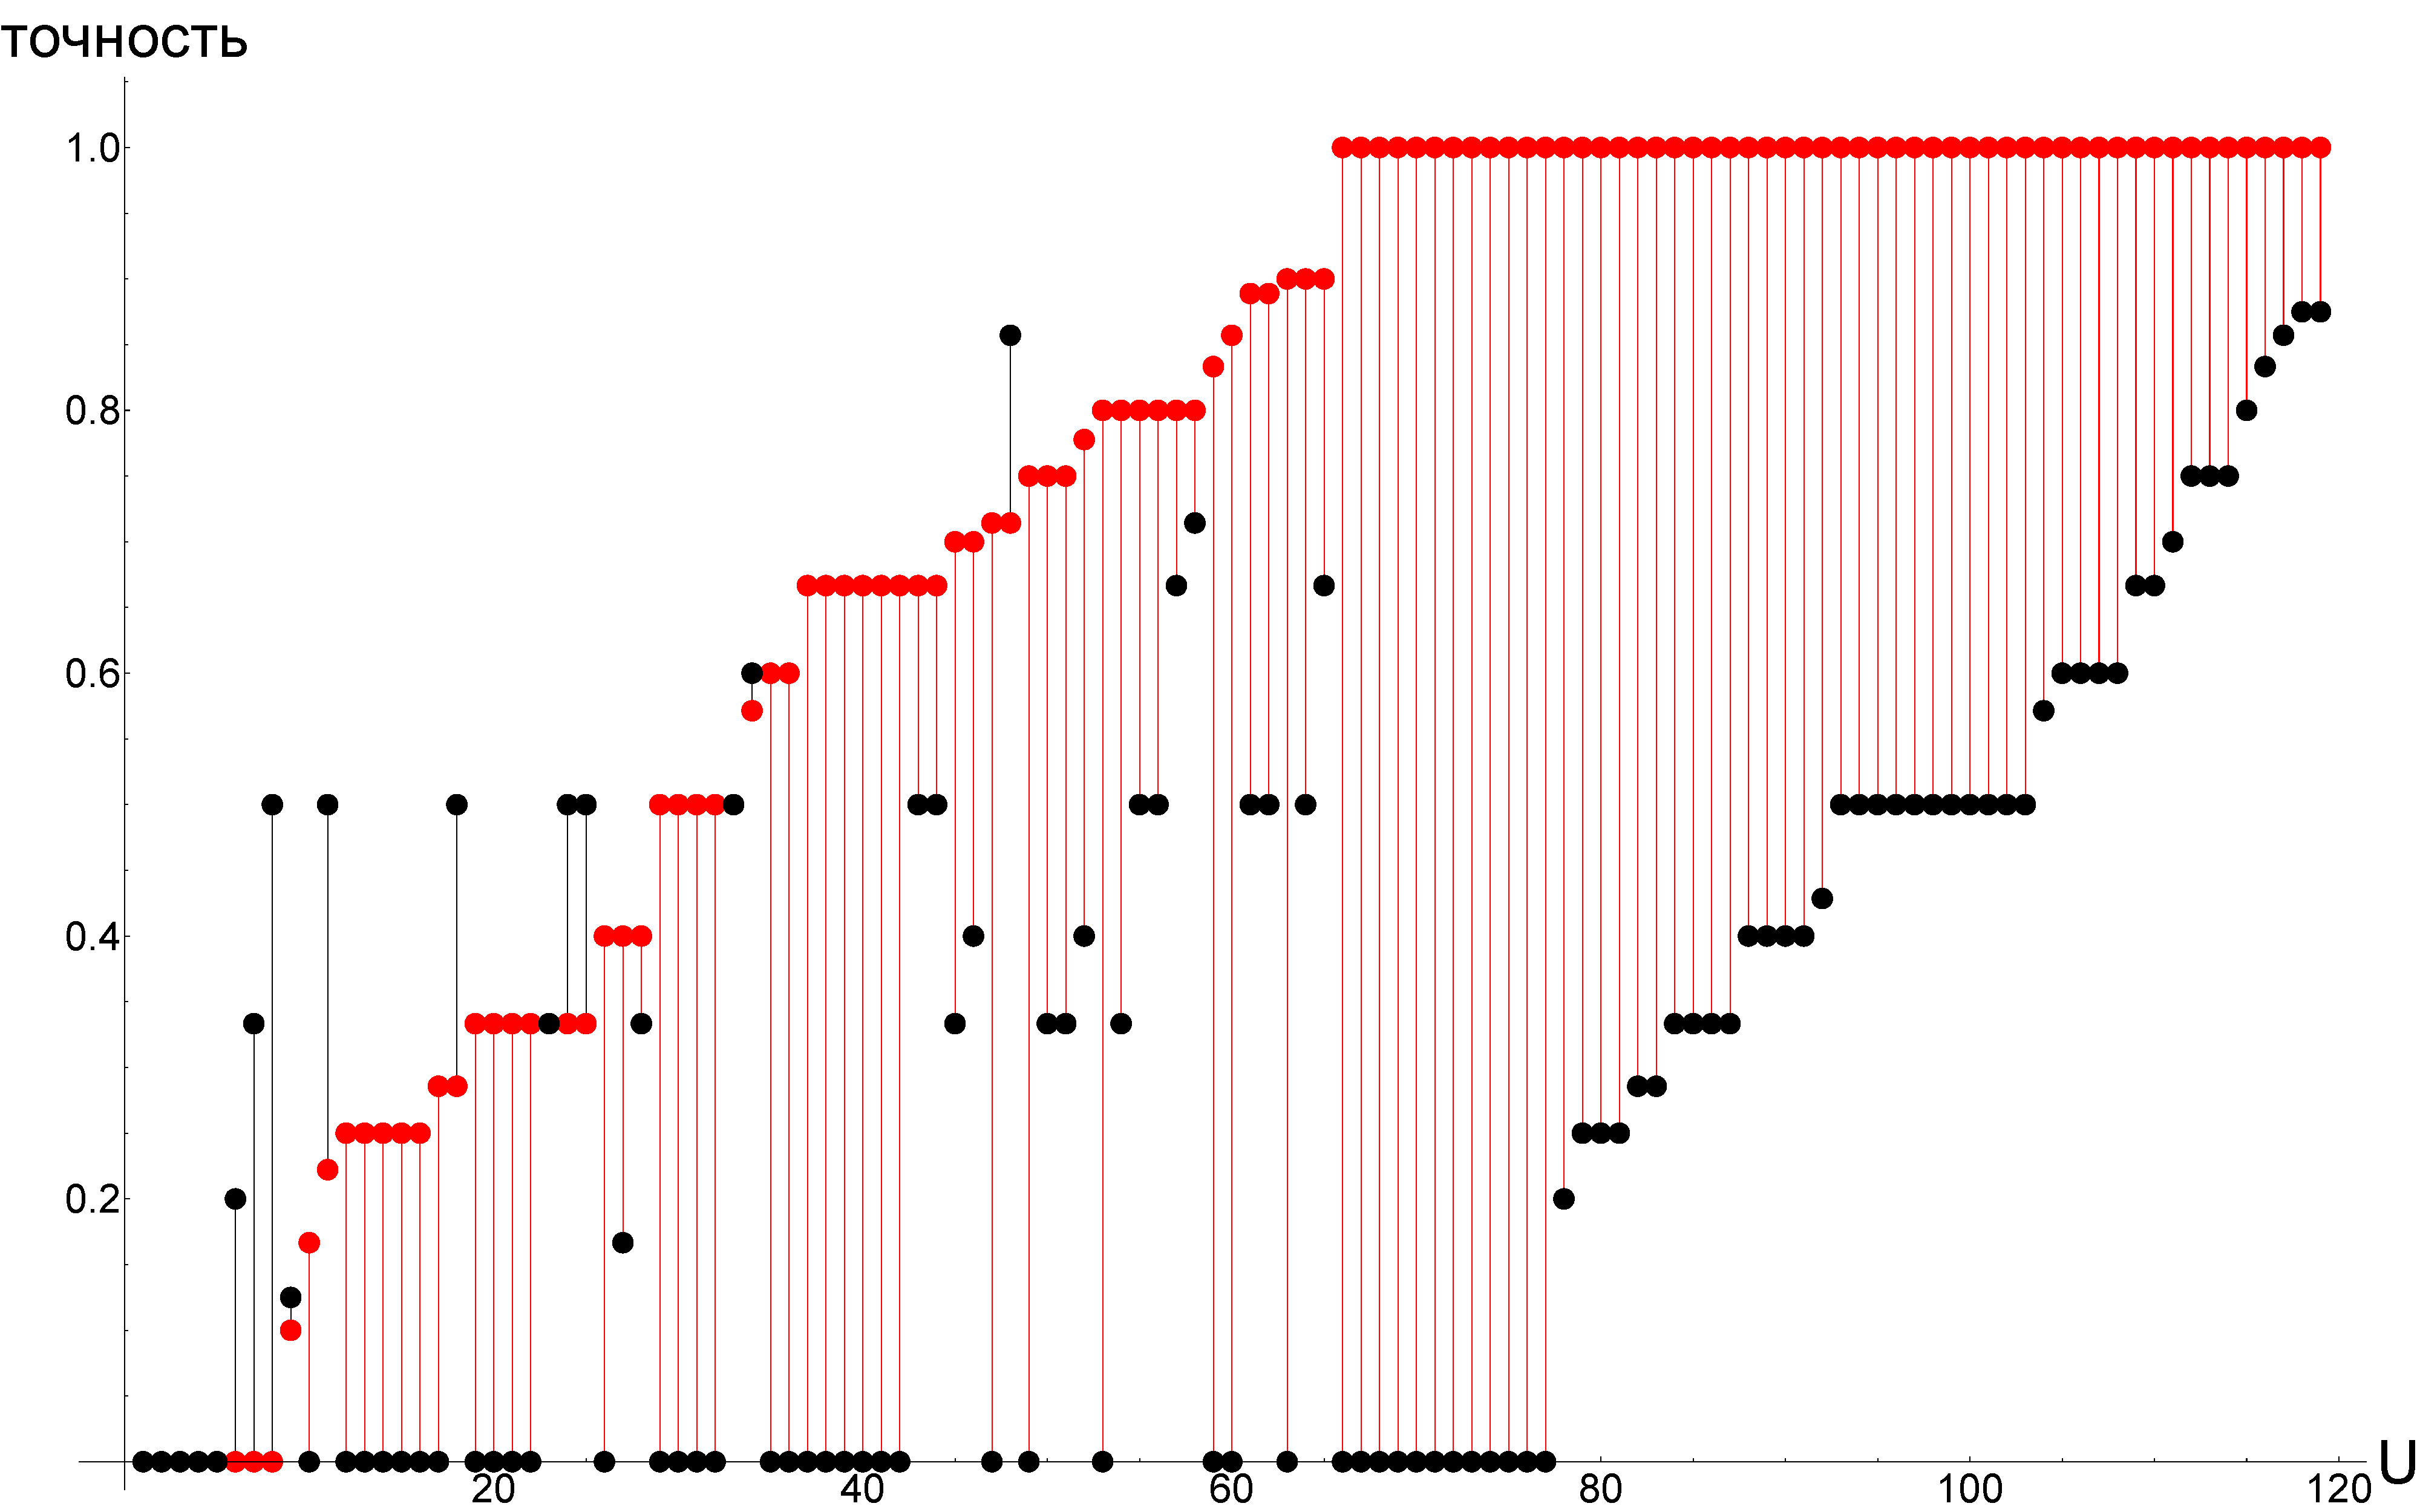
\includegraphics[width=7in,height=4in]{pics/results/ib_method_in_ib_and_fuzzy_model.pdf}
\end{center}
\end{figure}

\begin{table}[H]
	\caption{Средняя точность решений при применении правила вывода $\Pi_{O}$ в нечеткой модели и ООМ}
  \label{tbl:topn_hamming}
  \begin{center}
	\begin{tabular}{|c|c|}
	  \hline
		Модель& Точность \\ \hline
		ООМ&0,627 \\ \hline
		Нечеткая&0,312 \\ \hline
	\end{tabular}
  \end{center}
\end{table}

Практические результаты подтверждают вывод (\ref{trm:fuz-eff-oom}) о том, что
применение $\Pi_O$ в нечеткой модели более эффективно по критерию качества,
чем применение того же правила в АКМ.

\subsubsection{Применение правила вывода нечеткой модели для решения задачи
$topN$}
В данном пункте приведем и сравним результаты решения задачи $topN$, полученные:
\begin{enumerate}
	\item в ООМ:
		\begin{itemize}
			\item
			стандартный алгоритма решения задачи
			$topN$ (\ref{alg:topn-solve-ors}), основанный на
			правиле вывода $\Pi_O$;
			\item
			пороговое значение $\Delta_i$ равно $0,9$;
			\item
		применяемая мера сходства --- косинус угла (\ref{sim-cos})
		между контентами, которые представляются в ООМ в виде векторов.
		\end{itemize}
	\item
		\begin{itemize}
			\item
			алгоритма решения задачи
			$topN$ (\ref{alg:fuz-topn}), основанный на
			правиле вывода $\Pi_f$;
		\end{itemize}
\end{enumerate}


\begin{figure}[H]
	\caption{Качество решений задачи $topN$ при использовании $\Pi_O$ в ООМ и
	$\Pi_f$ в НРС}
	\label{pic:topn_pio_pif}
	\begin{center}
		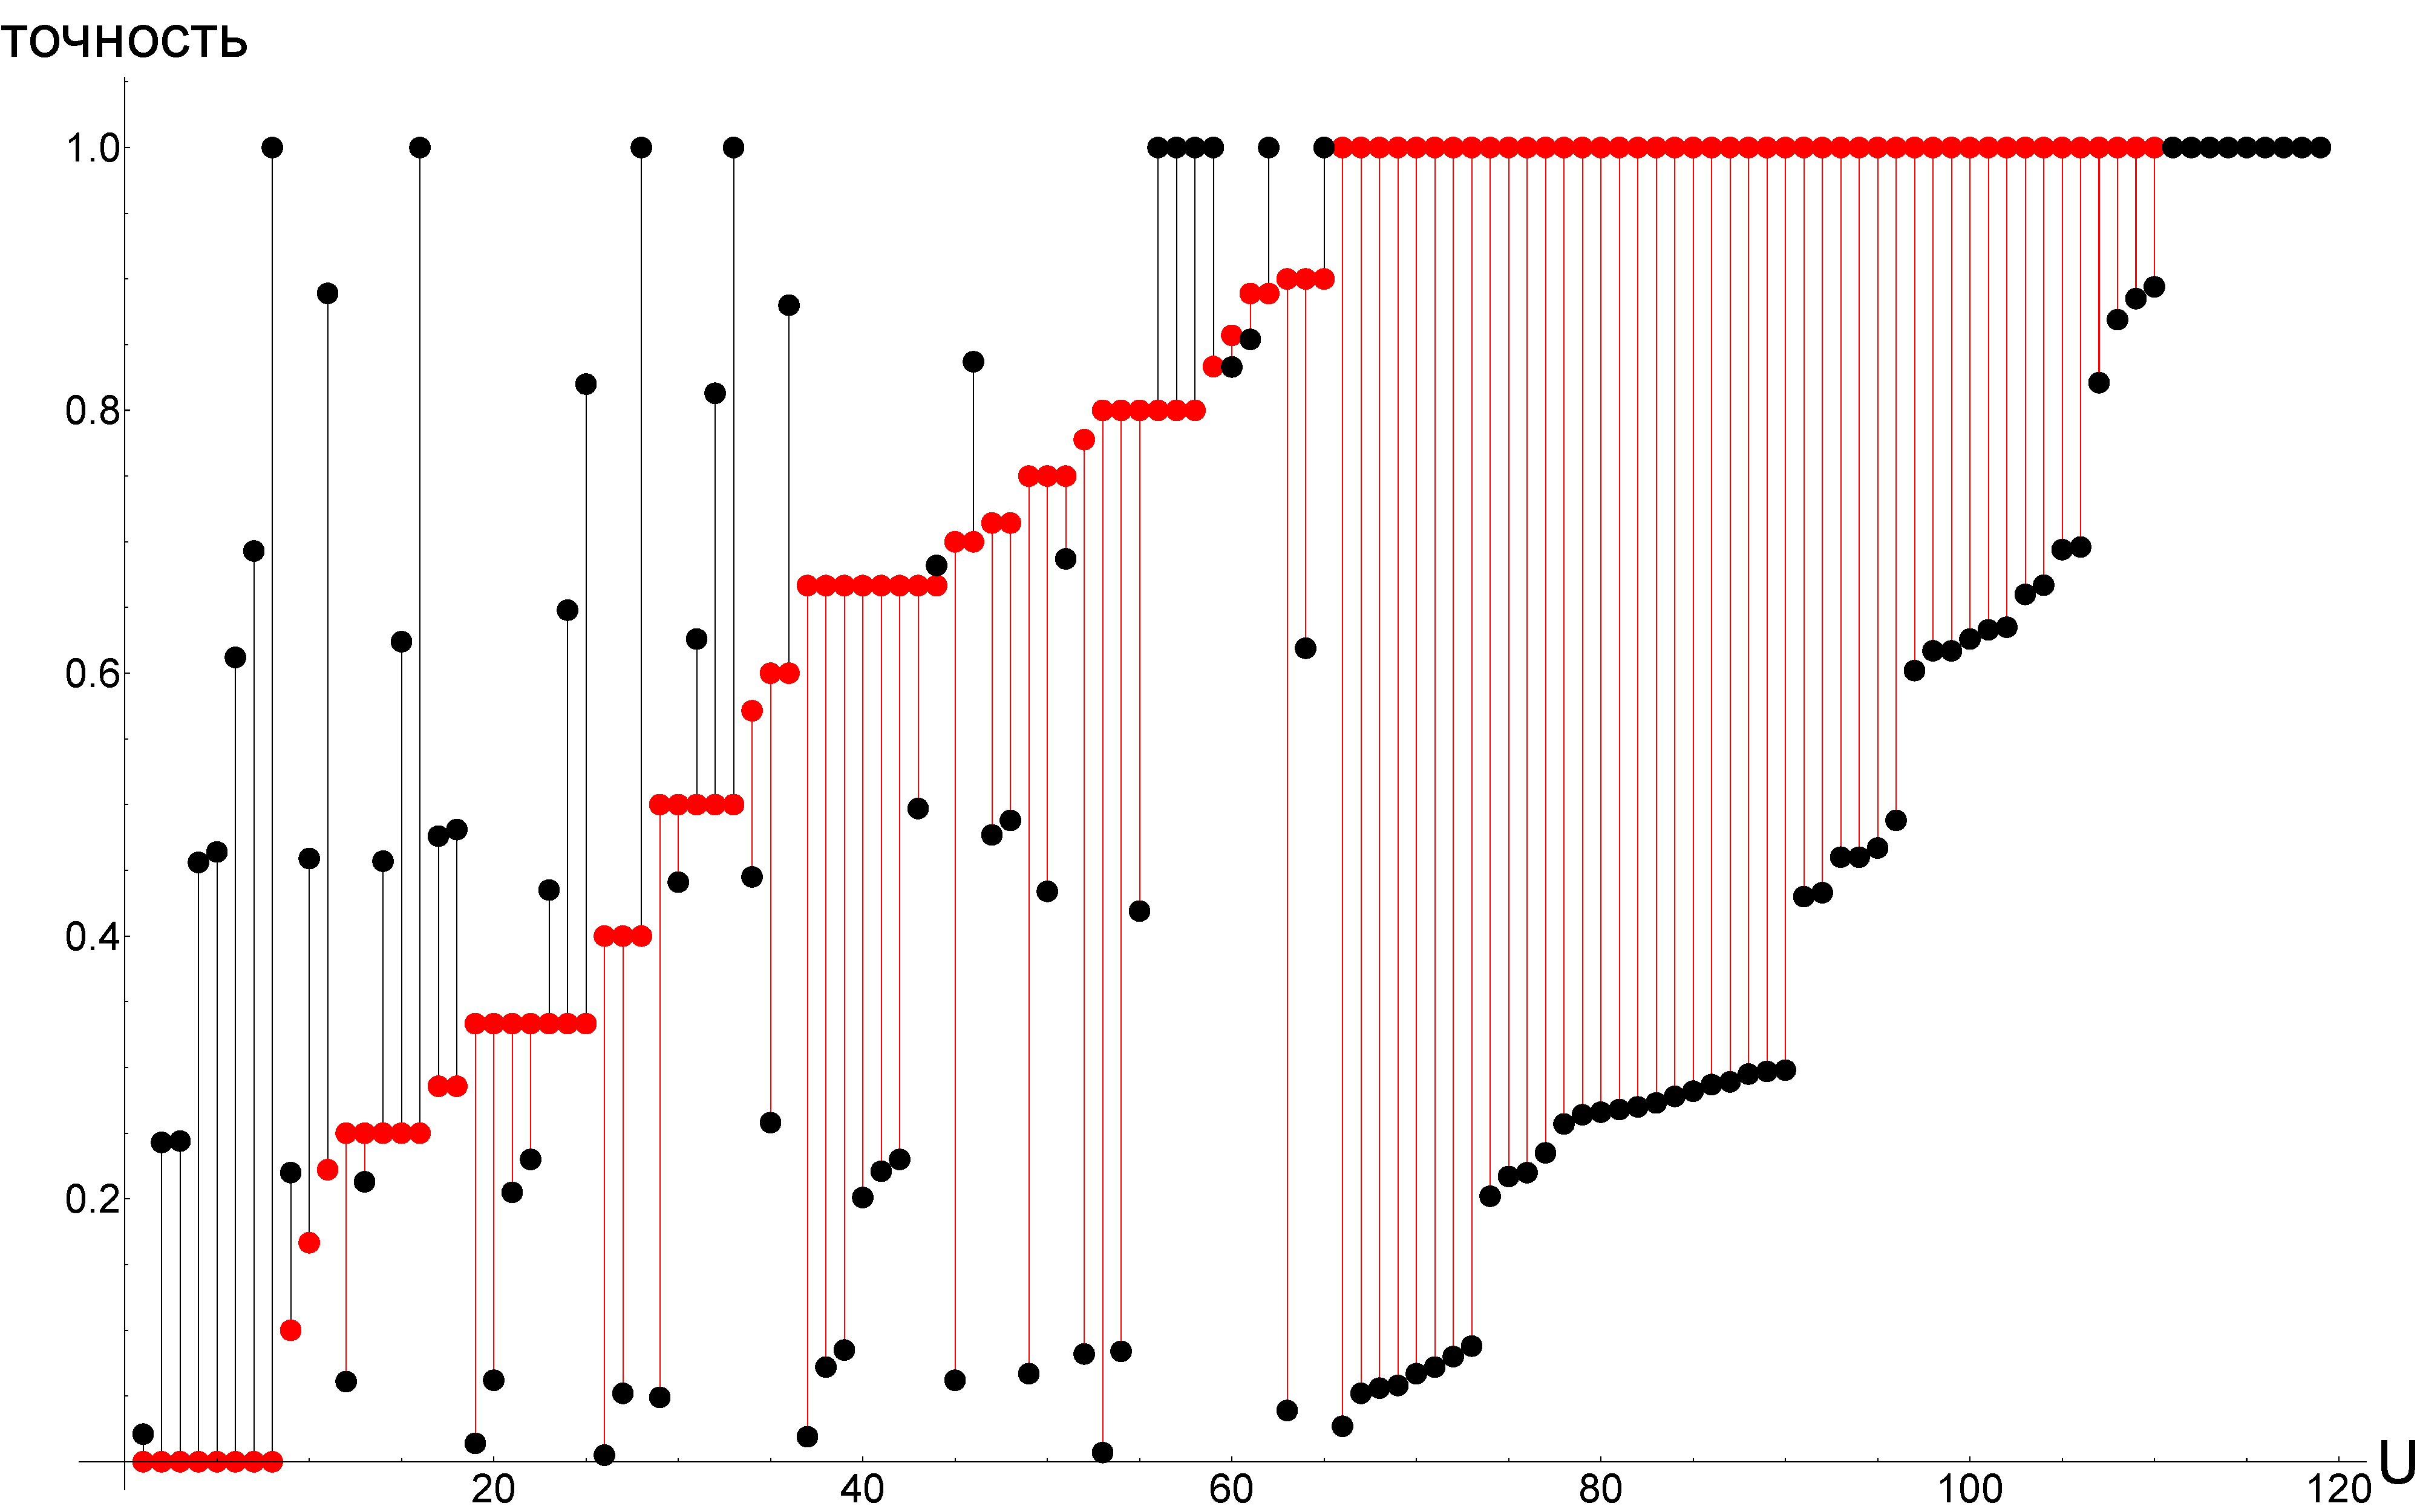
\includegraphics[width=7in,height=4in]{pics/results/topn_oom_fuzz.pdf}
\end{center}
\end{figure}

\begin{table}[H]
	\caption{Средняя точность решений в ООМ и нечеткой модели при применении
	$\Pi_f$}
  \begin{center}
	\label{tbl:topn_fuz}
	\begin{tabular}{|c|c|}
	  \hline
		Модель/Правило вывода & Точность \\ \hline
		ООМ/$\Pi_{O}$&0,627 \\ \hline
		Нечеткая/$\Pi_{f}$&0,420 \\ \hline
	\end{tabular}
  \end{center}
\end{table}


На Рис. \ref{pic:topn_pio_pif} приведены результаты решения
задачи $topN$ при применении $\Pi_O$ в ООМ и нечеткой модели.
Черным цветом обозначены результаты решения в нечеткой модели.
Видно, что в большинстве случаев нечеткая модель более эффективна
по критерию качества. В обратных ситуациях предпочтения пользователя
неоднородны, и $\delta_c$ для таких пользователей определена так, что
$|\rho(u, i) - \rh(u, i)| > \varepsilon_p$.

Практические результаты подтверждают вывод (\ref{trm:fuz-eff-extension}) о том,
что нечеткая модель является эффективным расширением АКМ по критерию качества.


\subsection{Задача прогнозирования}
Результаты представляются графиком и таблицей для каждого пункта.
Координатой оси $X$ является идентификатор пользователя, координатой
оси $Y$ является значение оценки качества.
В качестве функции $\eit$ использовалась функция
NMAE \ref{nmae}.
Другие функции рассматривались так же, но между
функциями одного класса существует корреляция и приведение других графиков
оказывается избыточным.

На графиках представляются данные по двум методам тестирования. Для наглядности
результирующие данные были отсортированы по значениям оценки качества,
принадлежащим первому методу (в каждой паре точек, которые находятся на одной
вертикали, идентификаторы пользователей совпадают).

В таблицах представлены средние значения оценок точности по всем пользователям.

Для проведения тестов данного пункта исходные данные были
стандартно разбиты на тестовое и обучающее множество по следующему принципу:
разбиение проводилось случайно, в обучающее множество входит
80\% данных, в тестовое --- оставшиеся 20\%. В тестировании участвовало
подмножество $P^{\prime} \subset P, P^{\prime} = \{(u, i, \rho(u, i)):
\rho(u, i) = 1\}$.

\subsubsection{Влияние свойства транзитивности на СОМ при решении задачи
прогнозирования}
В данном пункте приведем и сравним результаты решения задачи $pred$, полученные:
\begin{enumerate}
	\item  в СОМ при следующих параметрах:
		\begin{itemize}
			\item
			стандартный алгоритма решения задачи
			$pred$ (\ref{alg:p-srs}), основанный на
			правиле вывода $\Pi_C$;
			\item
			пороговое значение $\Delta_u$ равно $0,9$;
			\item
		применяемая мера сходства --- коэффициент корреляции Пирсона
				(\ref{pearson}).
		\end{itemize}
	\item  в СОМ при следующих параметрах:
		\begin{itemize}
			\item
			стандартный алгоритма решения задачи
			$pred$ (\ref{alg:p-srs}), основанный на
			правиле вывода $\Pi_C$;
			\item
			пороговое значение $\Delta_u$ равно $0,49$;
			\item
		применяемая мера сходства --- коэффициент корреляции Пирсона
				(\ref{pearson}).
		\end{itemize}
\end{enumerate}

При $\Delta_u = 0,9$ вероятность того, что $(u \rt v) \wedge (v \rt z)
\Rightarrow (u \rt z)$, выше, чем при $\Delta_u = 0,49$.
На Рис. \ref{pic:predtrans} приведены результаты решений задачи $topN$ при
различных пороговых значениях. Черным цветом приведены результаты для
$\Delta_u = 0,9$, красным --- для $\Delta_u = 0,49$.
Видно, что при $\Delta_u = 0,9$ результаты решений эффективней, так
как большинство точек, соответствующих $\Delta_u = 0,9$ проходит ниже точек,
соответствующих $\Delta_u = 0,49$, что также подтверждается табличными данными,
представленными в таблице (\ref{tbl:predtrans}).

Некоторые результаты при $\Delta_u = 0,9$ хуже, чем при
$\Delta_u = 0,49$. Это происходит для тех пользователей,
для которых характерно свойство неоднородности.

\begin{figure}[H]
	\caption{Влияние свойства транзитивности на СОМ при решении задачи $pred$}
	\label{pic:predtrans}
	\begin{center}
		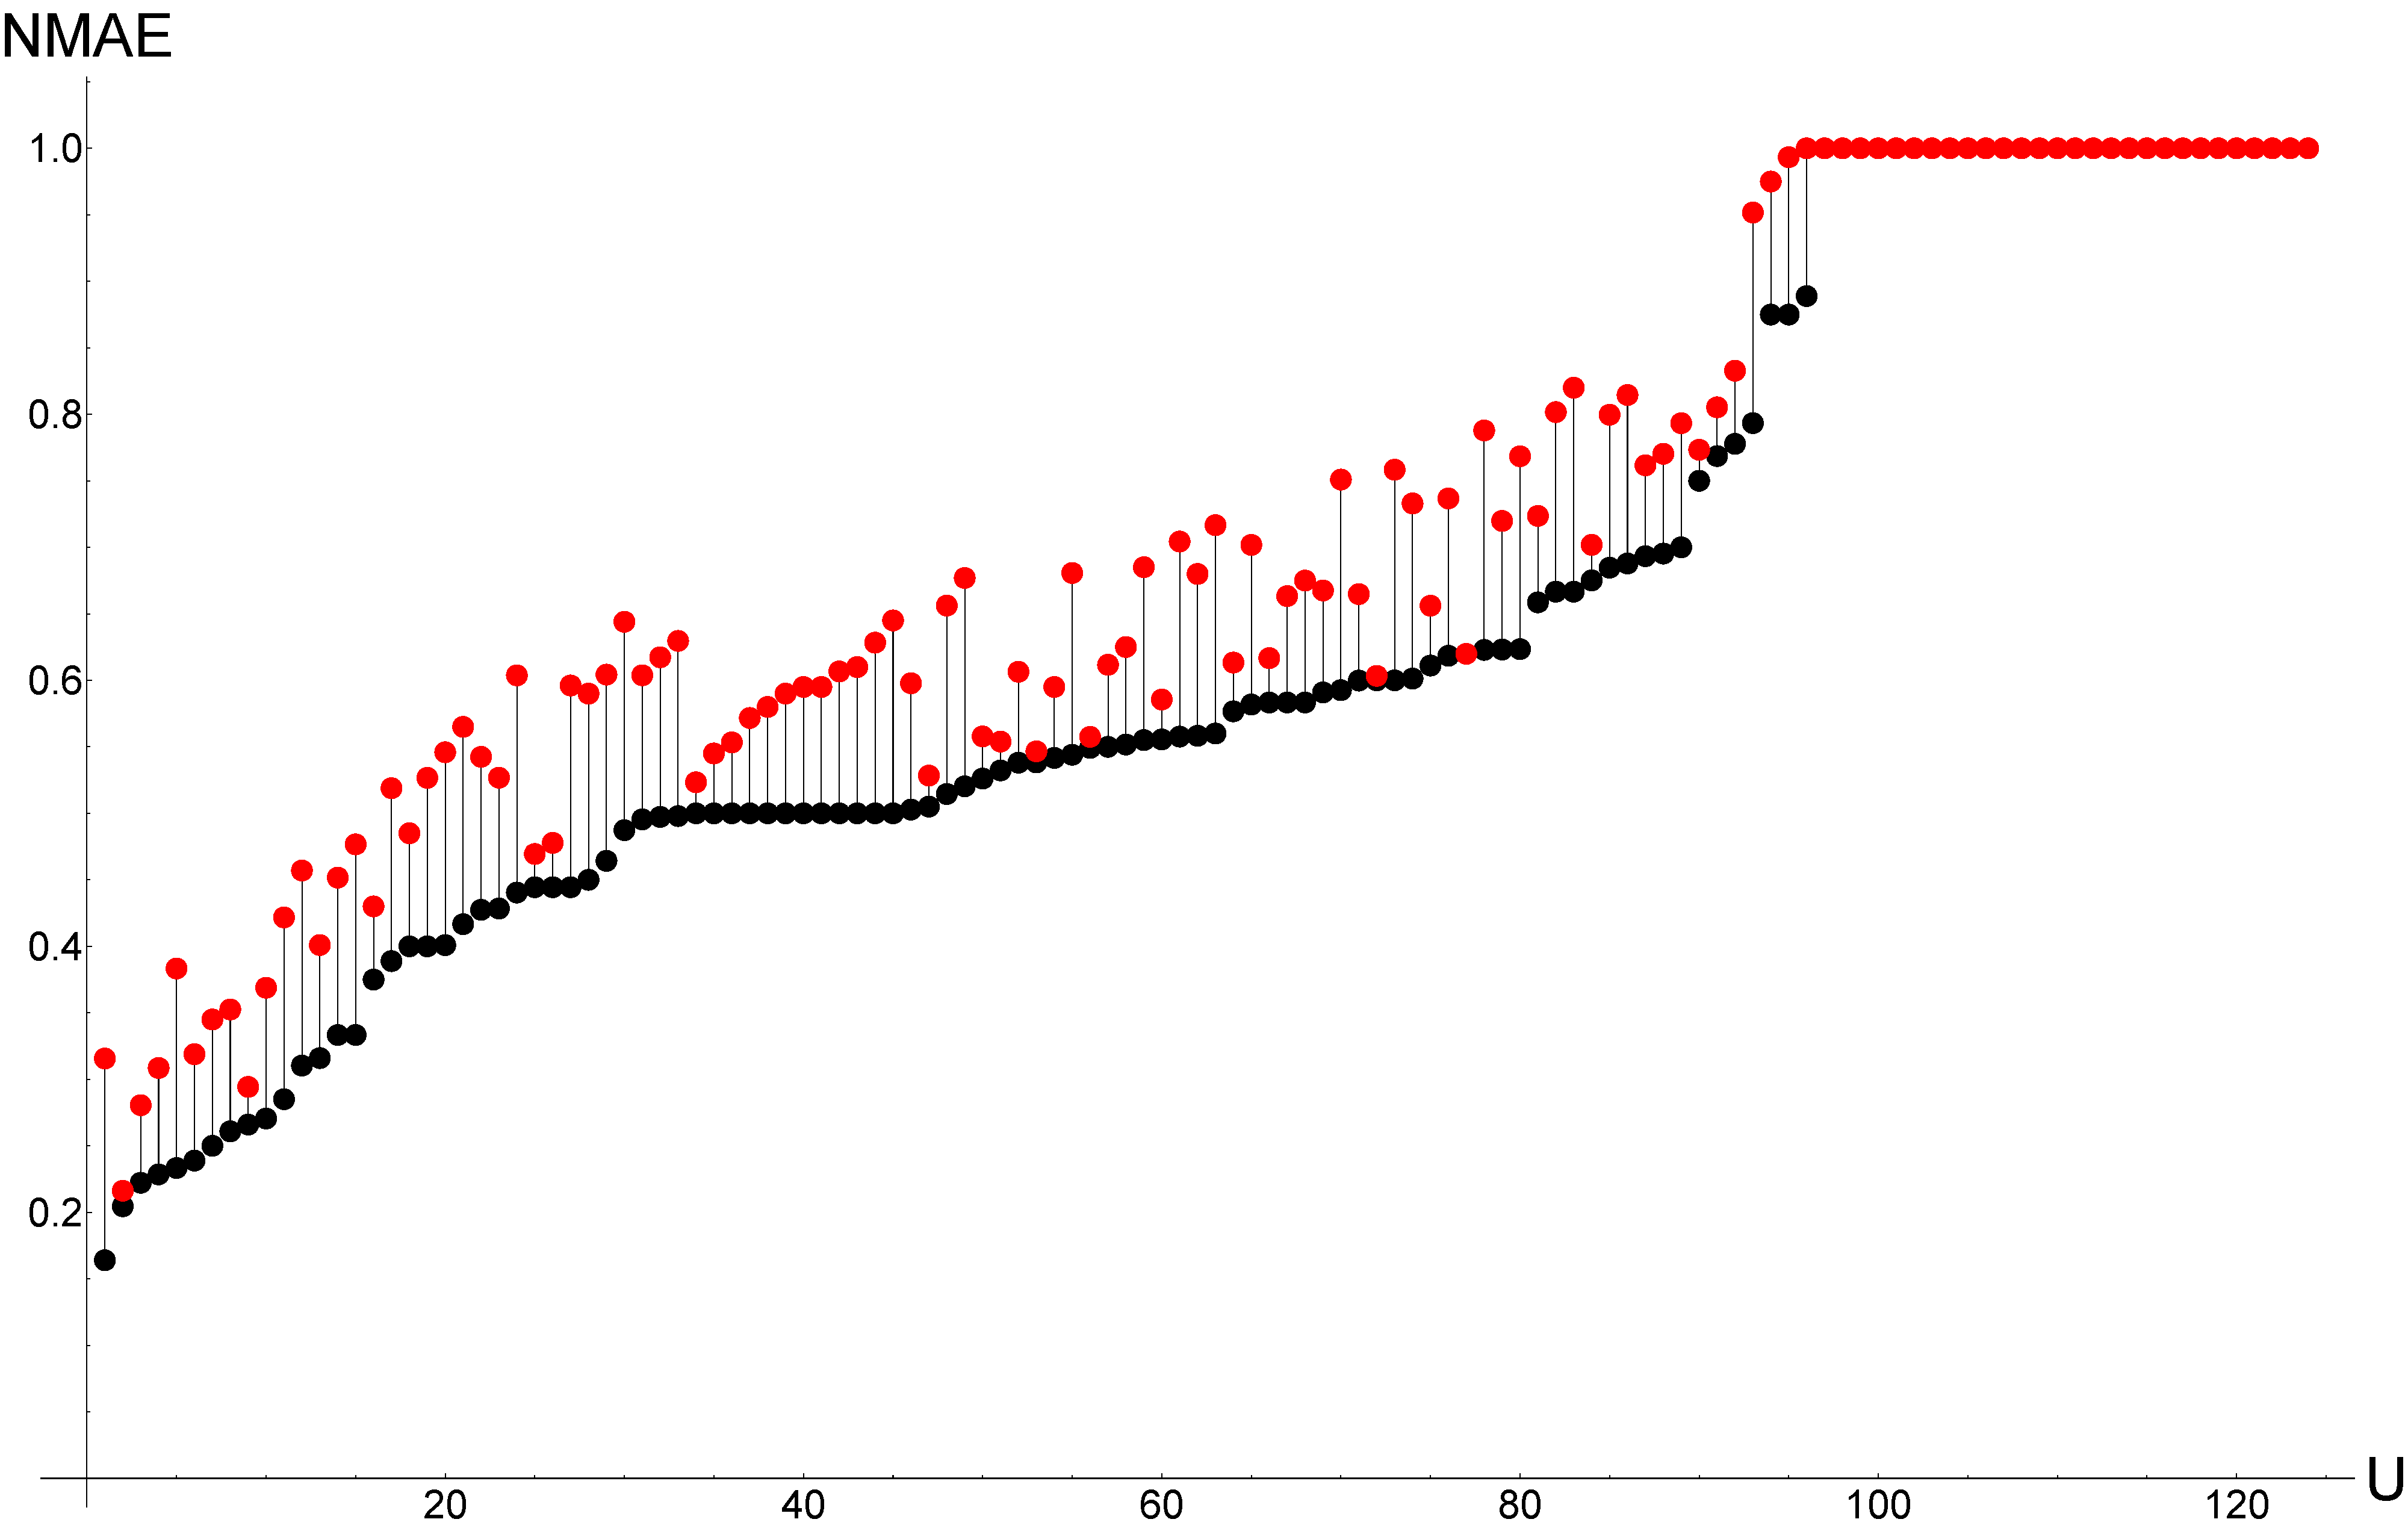
\includegraphics[width=7in,height=4in]{pics/results/ub_transitivity.pdf}
\end{center}
\end{figure}

\begin{table}[H]
	\caption{Влияние свойства транзитивности на СОМ при решении задачи $pred$}
  \label{tbl:predtrans}
  \begin{center}
	\begin{tabular}{|c|c|}
	  \hline
		Пороговое значение & NMAE \\ \hline
		0,9&0,495 \\ \hline
		0,49&0,601 \\ \hline
	\end{tabular}
  \end{center}
\end{table}

\subsubsection{Применение правила вывода СОМ в коллаборативной и нечеткой
моделях}
В данном пункте приведем и сравним результаты решения задачи $topN$, полученные:
\begin{enumerate}
	\item  в СОМ при следующих параметрах:
		\begin{itemize}
			\item
			стандартный алгоритма решения задачи
			$pred$ (\ref{alg:p-srs}), основанный на
			правиле вывода $\Pi_C$;
			\item
			пороговое значение $\Delta_u$ равно $0,9$;
			\item
		применяемая мера сходства --- коэффициент корреляции Пирсона
		\end{itemize}
	\item в нечеткой при следующих параметрах:
		\begin{itemize}
			\item
			стандартный алгоритма решения задачи
			$pred$ (\ref{alg:p-srs}), основанный на
			правиле вывода $\Pi_C$;
			\item
				применяемая мера сходства --- обобщенное расстояние Хэмминга
				(\ref{fuz:rhi})
		\end{itemize}
\end{enumerate}

На Рис. \ref{pic:predpio} приведены результаты решения
задачи $topN$ при применении $\Pi_C$ в СОМ и нечеткой модели.
Черным цветом обозначены результаты решения в нечеткой модели.
Видно, что в большинстве случаев нечеткая модель более эффективна
по критерию качества. В обратных ситуациях предпочтения пользователя
неоднородны.
%, и $\delta_c$ для таких пользователей определена так, что
%$|\rho(u, i) - \rh(u, i)| > \varepsilon_p$.

\begin{figure}[H]
	\caption{Качество решений при применении правила вывода $\Pi_{C}$ в нечеткой модели и СОМ}
	\label{pic:predpio}
	\begin{center}
		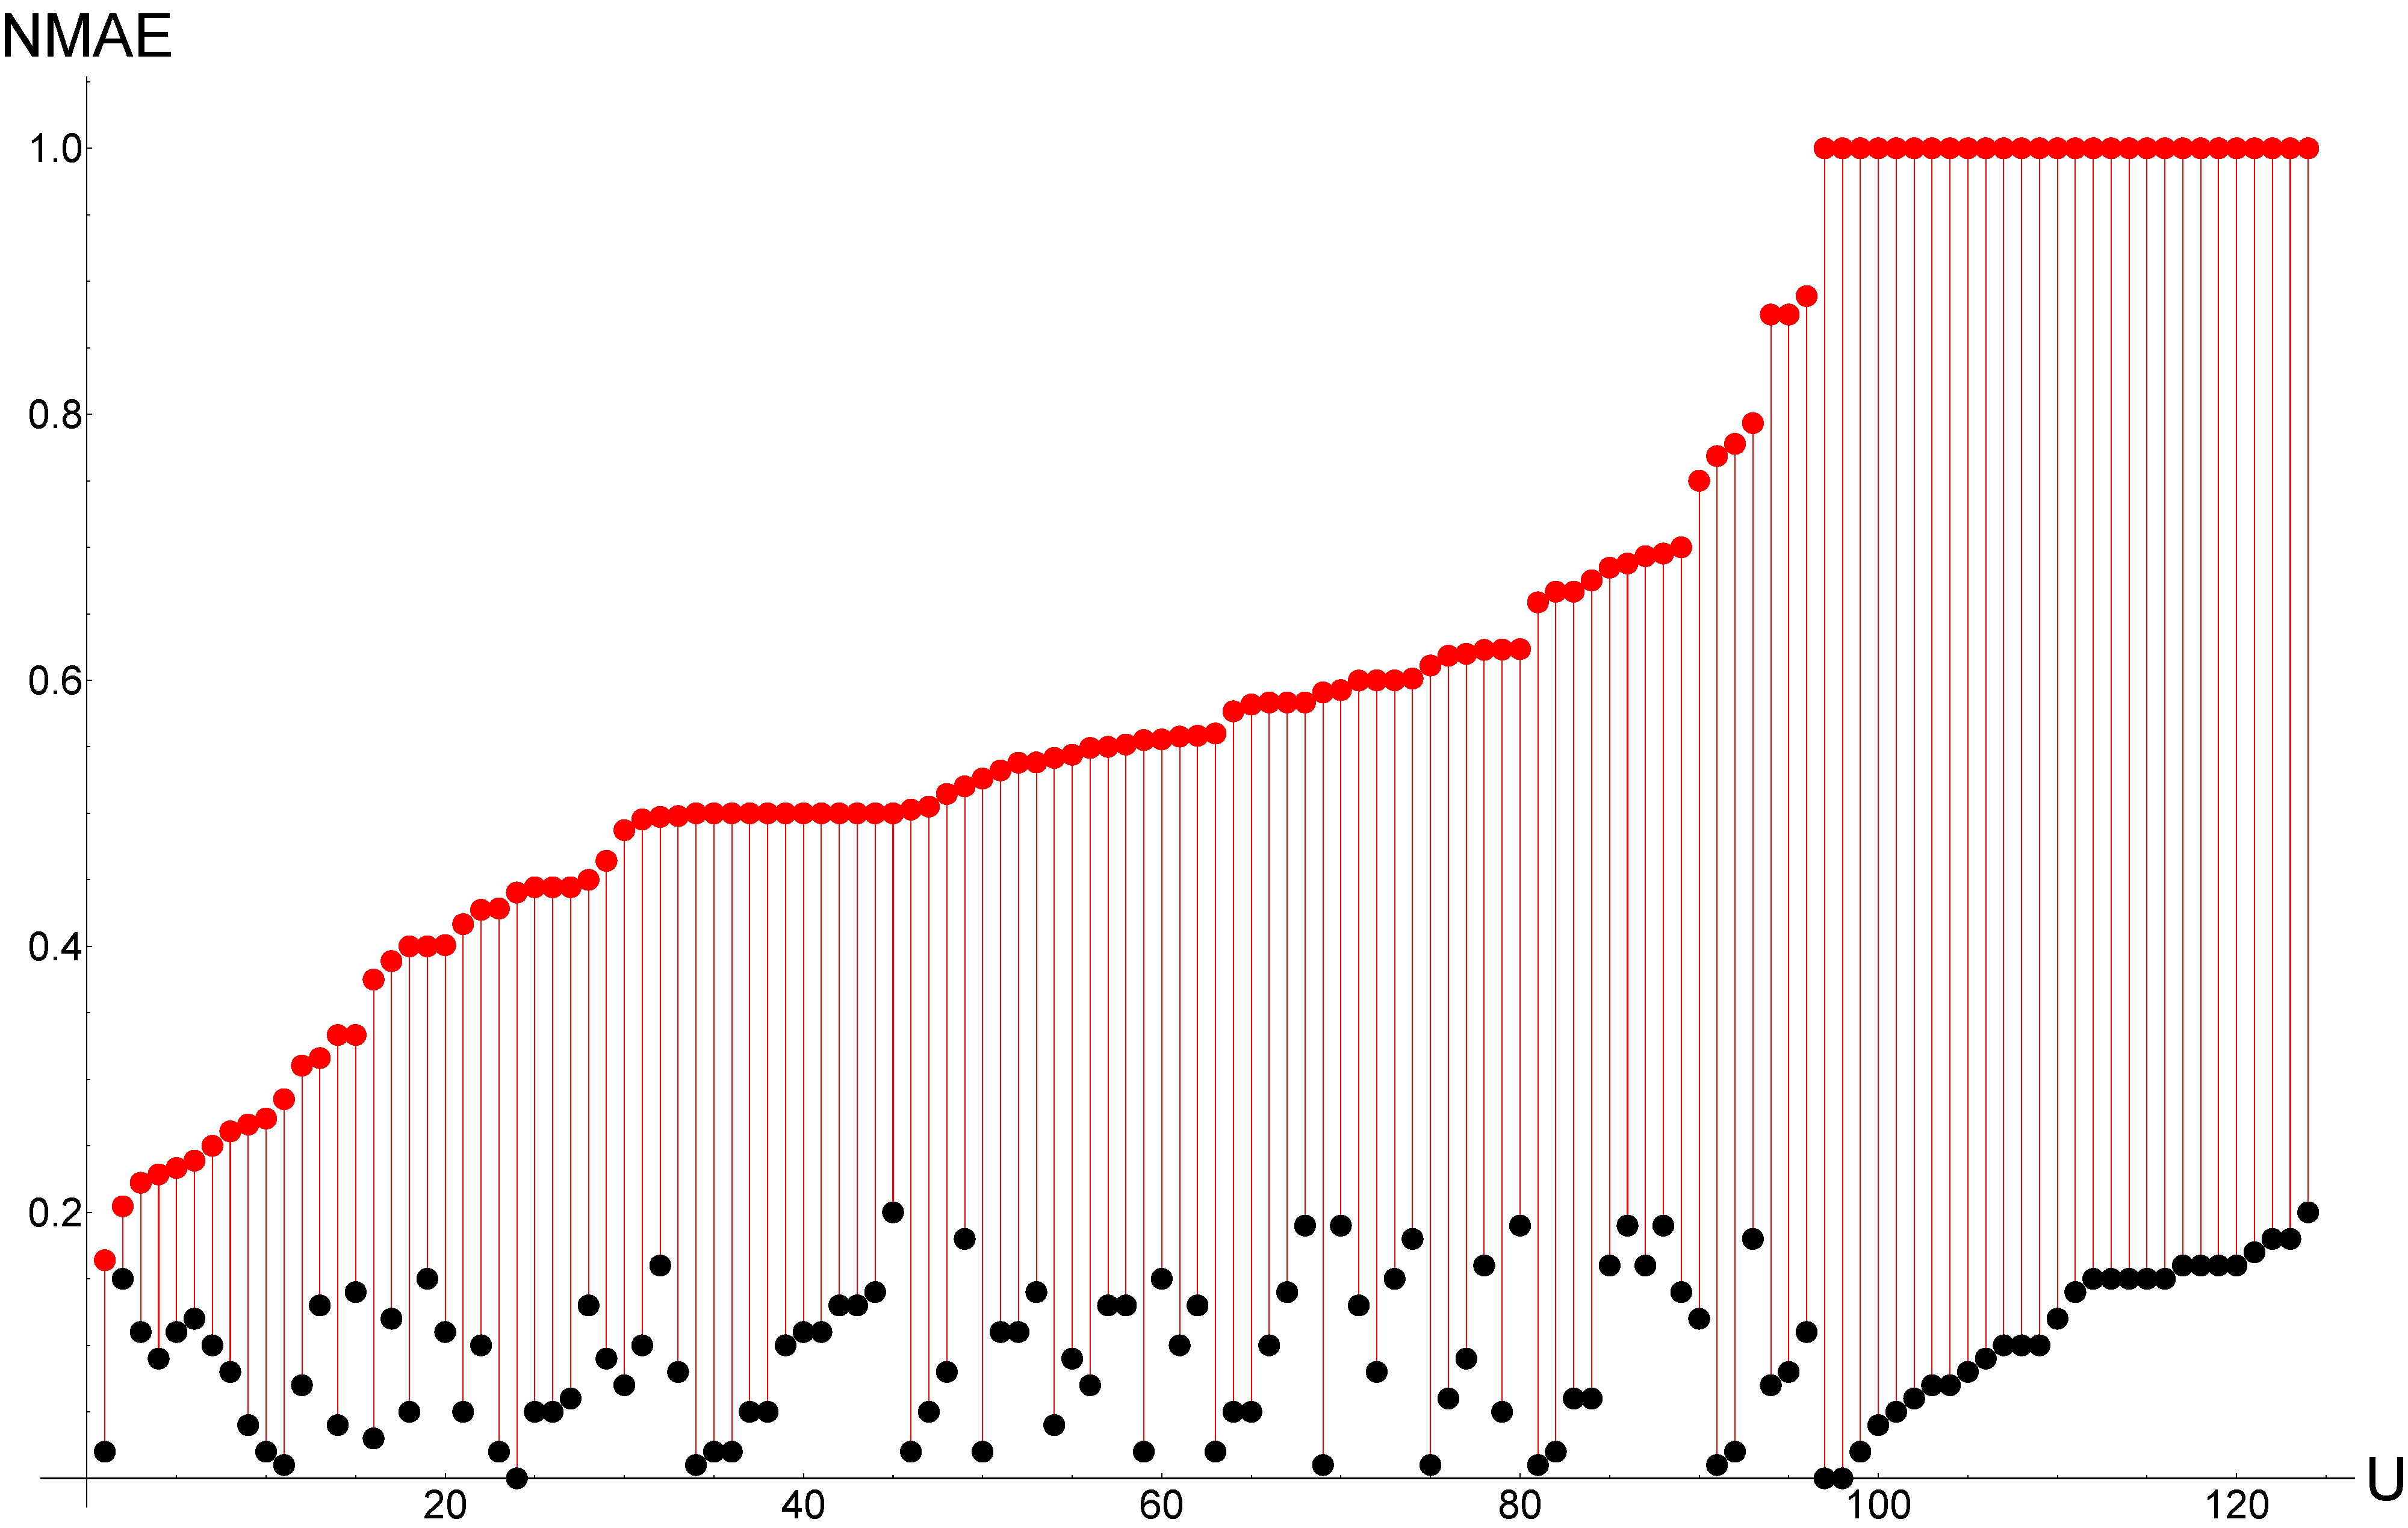
\includegraphics[width=7in,height=4in]{pics/results/ub_method_in_ub_and_fuzz_model.pdf}
\end{center}
\end{figure}

\begin{table}[H]
	\caption{Средняя точность решений при применении правила вывода $\Pi_{C}$ в нечеткой модели и СОМ}
  \label{tbl:predhamming}
  \begin{center}
	\begin{tabular}{|c|c|}
	  \hline
		Модель& Точность \\ \hline
		Нечеткая&0,001 \\ \hline
		COM&0,495\\ \hline
	\end{tabular}
  \end{center}
\end{table}

Практические результаты подтверждают вывод (\ref{trm:fuz-eff-com}) о том, что
применение $\Pi_C$ в нечеткой модели более эффективно по критерию качества,
чем применение того же правила в АКМ.

\subsubsection{Применение правила вывода нечеткой модели для решения задачи
$pred$}
В данном пункте приведем и сравним результаты решения задачи $pred$, полученные:
\begin{enumerate}
	\item в СОМ:
		\begin{itemize}
			\item
			стандартный алгоритма решения задачи
			$topN$ (\ref{alg:topn-solve-ors}), основанный на
			правиле вывода $\Pi_C$;
			\item
			пороговое значение $\Delta_u$ равно $0,9$;
			\item
		применяемая мера сходства --- косинус угла (\ref{sim-cos})
		между контентами, которые представляются в СОМ в виде векторов.
		\end{itemize}
	\item
		\begin{itemize}
			\item
			алгоритма решения задачи
			$pred$ (\ref{alg:fuz-p}), основанный на
			правиле вывода $\Pi_f$;
		\end{itemize}
\end{enumerate}


\begin{figure}[H]
	\caption{Качество решений задачи $pred$ при использовании $\Pi_C$ в СОМ и
	$\Pi_f$ в нечеткой модели}
	\label{pic:predpio_pif}
	\begin{center}
		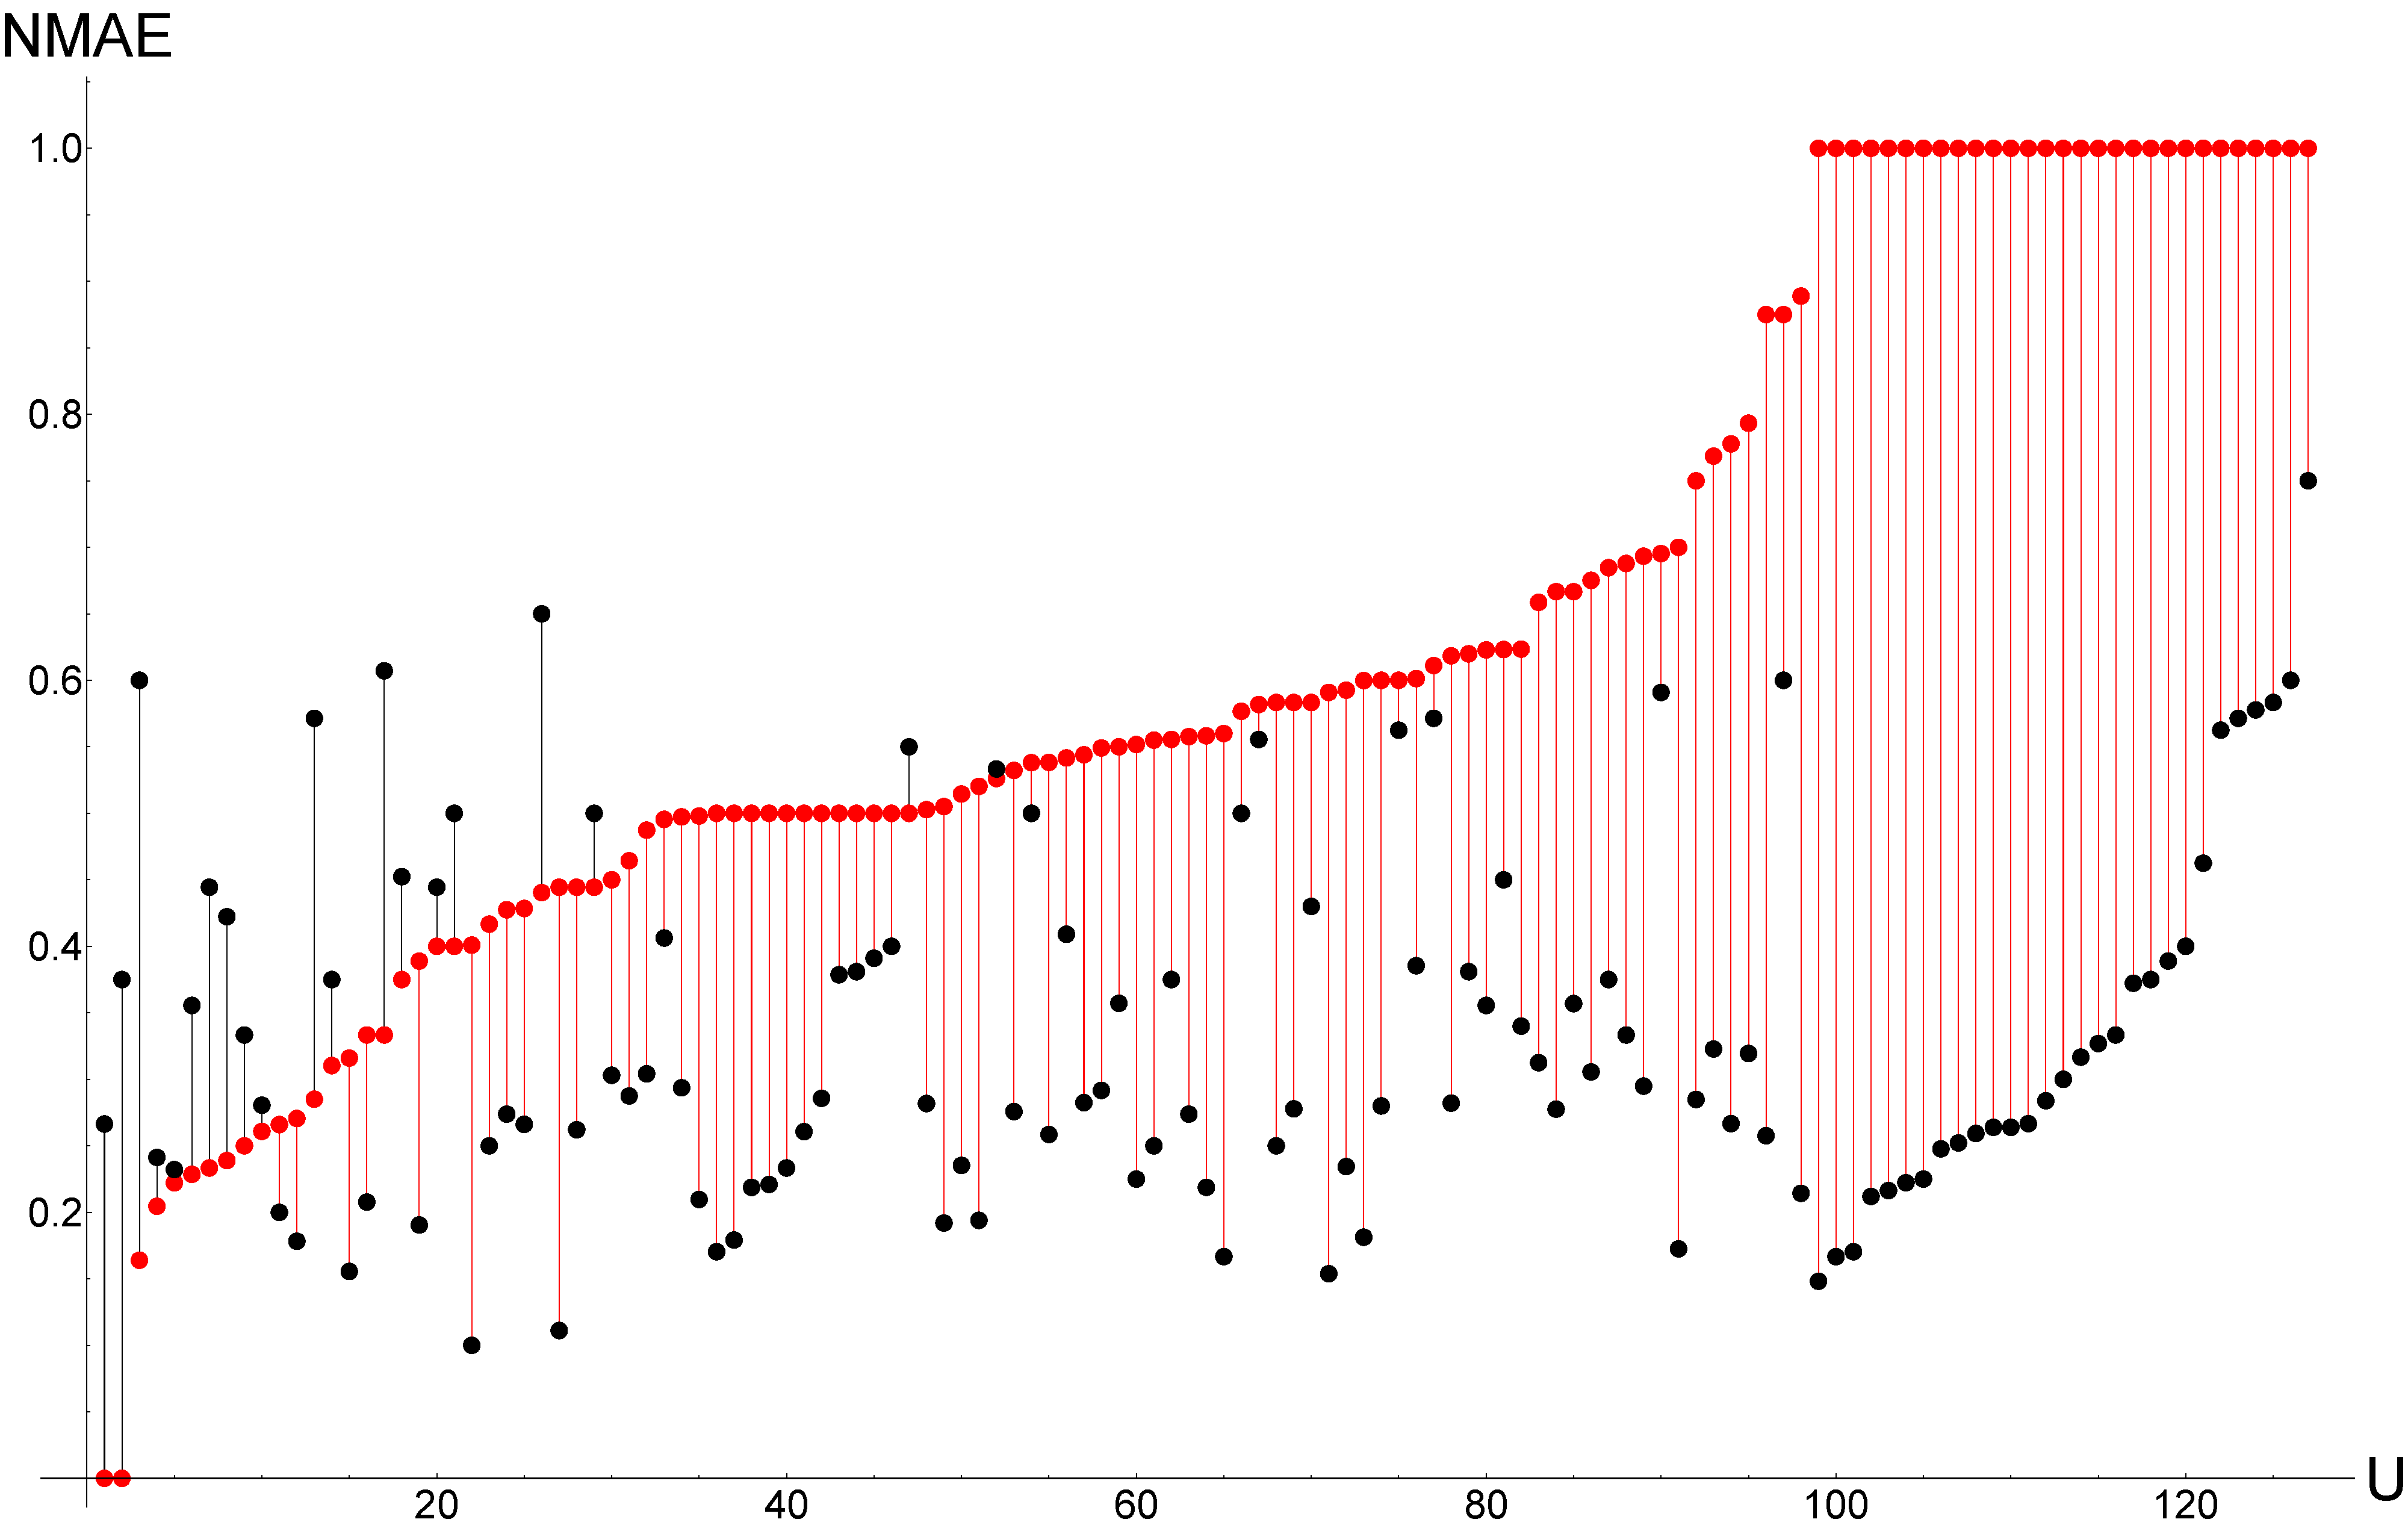
\includegraphics[width=7in,height=4in]{pics/results/ub_vs_fuzzy.pdf}
\end{center}
\end{figure}

\begin{table}[H]
	\caption{Средняя точность решений в СОМ и нечеткой модели при применении
	$\Pi_f$}
  \begin{center}
	\label{tbl:predfuz}
	\begin{tabular}{|c|c|}
	  \hline
		Модель/Правило вывода & Точность \\ \hline
		СОМ/$\Pi_{O}$&0,495\\ \hline
		Нечеткая/$\Pi_{f}$&0,334 \\ \hline
	\end{tabular}
  \end{center}
\end{table}


На Рис. \ref{pic:predpio_pif} приведены результаты решения
задачи $pred$ при применении $\Pi_C$ в СОМ и нечеткой модели.
Черным цветом обозначены результаты решения в нечеткой модели.
Видно, что в большинстве случаев нечеткая модель более эффективна
по критерию качества. В обратных ситуациях предпочтения пользователя
неоднородны, и $\delta_c$ для таких пользователей определена так, что
$|\rho(u, i) - \rh(u, i)| > \varepsilon_p$.

Практические результаты подтверждают вывод (\ref{trm:fuz-eff-extension}) о том,
что нечеткая модель является эффективным расширением АКМ по критерию качества.


%
\section{Сравнение моделей по критерию стабильности}
\subsection{Влияние свойства динамики исходных данных}

В аналитической главе говорилось о влиянии свойства динамики
данных (\ref{ass:dynamic}) на качество решения в СОМ, а точнее на выполнение
эвристического утверждения СОМ (\ref{srs-assert}). Для теста данного пункта
была произведена имитация проявления свойства динамики, для этого
исходные данные были разбиты не стандартно в пропорции 80 к 20, а
в пропорции 40 к 60, то есть в обучающее множество попало 40\%
данных, остальные --- в тестовое. При таком разбиении вероятность
того, что $u \ru v$ на обучающем множестве выполняется, но на тестовом --- нет,
высока.


Результаты представлены в следующих формах:
\begin{enumerate}
	\item таблицей <<Влияние свойства динамики на качество решения при применении
	$\Pi_C$ в СОМ>> (\ref{tbl:dynamic-com}), в которой указаны
	средние значения $NMAE$ при решении задачи прогнозирования
	в СОМ и при использовании стандартного алгоритма
	на стандартно разбиении и на разбиении 40/60. Значения
	$NMAE$ для разбиения 40/60 выше, что говорит о зависимости
	качества решения от выполнения эвристического утверждения и его
		зависимости от свойств исходных данных;

	\item таблицей <<Влияние свойства динамики на качество решения при применении
	$\Pi_C$ в нечеткой модели>> (\ref{tbl:dynamic-com}), в которой указаны
	средние значения $NMAE$ при решении задачи прогнозирования
	в нечеткой модели и при использовании стандартного алгоритма
	на стандартно разбиении и на разбиении 40/60. Значения
	$NMAE$ для разбиения 40/60 выше, что говорит о зависимости
	качества решения от выполнения эвристического утверждения и его
	зависимости от свойств исходных данных независимо от используемой модели;

	\item таблицей <<Влияние свойства динамики на качество решения при применении
	$\Pi_f$ в нечеткой модели>> (\ref{tbl:dynamic-fuz-com}), в которой указаны
	средние значения $NMAE$ для стандартного разбиения и 40/60
	при решении задачи прогнозирования в нечеткой модели и при использовании
	алгоритма $\Pi_f$, основанного на $\Pi_f$.
	В таблице (\ref{tbl:dynamic-fuz-com}) среднее значение $NMAE$, соответствующее
	решению задачи на разбиении 40/60 больше, чем среднее значение $NMAE$
	на стандартном разбиении
	что свидетельствует о влиянии свойства динамики на качество решения
	при использовании $\Pi_f$ в нечеткой модели. Проявление влияния следует из
	того, что функция $\delta_c$ составлена по данным, которые принадлежат
	множеству $P$. Но, несмотря на влияние, эффективность нечеткой модели
	при применении $\Pi_f$
	снижается не столь стремительно как в случае применения $\Pi_C$
	и дает в условиях динамики более эффективный результат,
	что подтверждает теоретический вывод о том, что нечеткая
	модель более эффективна по критерию стабильности.
\end{enumerate}

\begin{table}[h]
	\caption{Влияние свойства динамики на качество решения при применении
	$\Pi_C$ в СОМ}
  \begin{center}
	\label{tbl:dynamic-com}
	\begin{tabular}{|c|c|}
	  \hline
		Разбиение & NMAE \\ \hline
		80/20 & 0,495 \\ \hline
		40/60 & 0,634 \\ \hline
	\end{tabular}
  \end{center}
\end{table}

\begin{table}[h]
	\caption{Влияние свойства динамики на качество решения при применении
	$\Pi_C$ в нечеткой модели}
  \begin{center}
	\label{tbl:dynamic-fuz-com}
	\begin{tabular}{|c|c|}
	  \hline
		Разбиение & NMAE \\ \hline
		80/20$\Pi_{O}$&0,001 \\ \hline
		40/60$\Pi_{f}$&0,420 \\ \hline
	\end{tabular}
  \end{center}
\end{table}

\begin{table}[h]
	\caption{Влияние свойства динамики на качество решения при применении
	$\Pi_f$ в нечеткой модели}
  \begin{center}
	\label{tbl:dynamic-fuz}
	\begin{tabular}{|c|c|}
	  \hline
		Разбиение & NMAE \\ \hline
		80/20$\Pi_{O}$&0,334 \\ \hline
		40/60$\Pi_{f}$&0,398 \\ \hline
	\end{tabular}
  \end{center}
\end{table}
Практические результаты подтверждают теоретические выводы о том,
что нечеткая модель при применении $\Pi_f$ более эффективна по критерию
стабильности (\ref{trm:fuz-eff-extension-stab}).

% hetero
\subsection{Влияние свойства неоднородности}
В аналитической главе говорилось о влиянии свойства неоднородности данных
(\ref{ass:hetero}) на качество решения в ООМ.
Свойство неоднородности в используемых для тестов данных
проявляется для некоторых пользователей. Это проявление
заключается в том, что пользователь высоко оценивает фильмы,
которые не схожи друг с другом по характеристикам. Например,
пользователь высоко оценивает фильм жанра <<comedy>> и фильм
жанра <<crime>>.

В данном пункте будут представлены результаты теста, которые
проводились на подмножестве таких пользователей $U^{\prime}$,
для которых проявляется свойство неоднородности в большей мере,
то есть процент объектов, между которыми не выполняется отношение близости
составляет больше 70\%.

Результаты представлены в следующих формах:
\begin{enumerate}
	\item таблицей <<Влияние неоднородности на ООМ>> (\ref{tbl:hetero-oom}), в которой указаны
	средние значения точности для множества пользователей $U$ и подмножества
	$U^{\prime}$ при решении задачи с помощью ООМ.
	В данной таблице (\ref{tbl:hetero-oom}) среднее значение точности, соответствующее
	решению задачи на подмножестве $U^{\prime}$, на порядок
	меньше значения точности решения для всего множества,
	что свидетельствует о влиянии свойства неоднородности на качество
	решения при использовании $\Pi_O$ в ООМ.

	\item таблицей <<Влияние неоднородности на нечеткую модель при применении $\Pi_O$>> (\ref{tbl:hetero-fuz-oom}), в которой указаны
	средние значения точности для множества пользователей $U$ и подмножества
	$U^{\prime}$ при решении задачи с помощью $\Pi_O$ в нечеткой модели.
	В данной таблице (\ref{tbl:hetero-fuz-oom}) среднее значение точности, соответствующее
	решению задачи на подмножестве $U^{\prime}$, на порядок
	меньше значения точности решения для всего множества,
	что свидетельствует о влиянии свойства неоднородности на качество решения
	при использовании $\Pi_O$ в нечеткой модели. В ООМ и нечеткой модели
	использовался один и тот же алгоритм, эффективность которого заметно
	снижается при проявлении свойства неоднородности, то есть независимо
	используемый алгоритм не дает эффективного результата.

	\item таблицей <<Влияние неоднородности на нечеткую модель при применении $\Pi_f$>> (\ref{tbl:hetero-fuz-oom}), в которой указаны
	средние значения точности для множества пользователей $U$ и подмножества
	$U^{\prime}$ при решении задачи с помощью $\Pi_O$ в нечеткой модели.
	В данной таблице (\ref{tbl:hetero-fuz-oom}) среднее значение точности, соответствующее
	решению задачи на подмножестве $U^{\prime}$, на порядок
	меньше значения точности решения для всего множества,
	что свидетельствует о влиянии свойства неоднородности на качество решения
	при использовании $\Pi_f$ в нечеткой модели. Проявление влияния следует из
	того, что функция $\delta_c$ составлена по данным, которые принадлежат
	множеству $P$. Но, несмотря на влияние, эффективность нечеткой модели
	при применении $\Pi_f$
	снижается не столь стремительно как в случае применения $\Pi_O$
	и дает в условиях неоднородности более эффективный результат,
	что подтверждает теоретический вывод о том, что нечеткая
	модель более эффективна по критерию стабильности.
\end{enumerate}

\begin{table}[h]
	\caption{Влияние неоднородности на ООМ}
  \begin{center}
	\label{tbl:hetero-oom}
	\begin{tabular}{|c|c|}
	  \hline
		Множество & Точность \\ \hline
		Все пользователи & 0,251 \\ \hline
		только те, для которых неоднородность выполняется & 0,108 \\ \hline
	\end{tabular}
  \end{center}
\end{table}

\begin{table}[h]
	\caption{Влияние неоднородности на нечеткую модель при применении $\Pi_O$}
  \begin{center}
	\label{tbl:hetero-fuz-oom}
	\begin{tabular}{|c|c|}
	  \hline
		Модель/Правило вывода & Точность \\ \hline
		ООМ/$\Pi_{O}$&0,644 \\ \hline
		Нечеткая/$\Pi_{f}$&0,277 \\ \hline
	\end{tabular}
  \end{center}
\end{table}

\begin{table}[h]
	\caption{Влияние неоднородности на нечеткую модель при применении $\Pi_f$}
  \begin{center}
	\label{tbl:hetero-fuz}
	\begin{tabular}{|c|c|}
	  \hline
		Свойство неоднородности проявляется & Точность \\ \hline
		Нет & 0,633 \\ \hline
		Да & 0,379 \\ \hline
	\end{tabular}
  \end{center}
\end{table}

Практические результаты подтверждают теоретические выводы о том,
что нечеткая модель при применении $\Pi_f$ более эффективна по критерию
стабильности (\ref{trm:fuz-eff-extension-stab}).


%%%%%%%%%%%%%%%%%%%%%%%%%%%%%%%%%%%%%%%%%%%%%%%%%%%%%%%%%%%%%%%%%%%%%%

\section{Сравнение моделей по критерию вычислительной сложности}
В качестве показателя вычислительной сложности алгоритма рассмотрим время,
которое затрачивается в среднем на решение задачи для одного пользователя.
Решение задачи $topN$ рассмотрим для $N = 10$, решение задачи прогнозирования
для одного прогнозируемого объекта. Алгоритмы использовались те же, что
применялись при определении качества решения, описанные выше.

Тесты проводились на следующем оборудовании:
\begin{itemize}
	\item ОС --- Ubuntu 16.04 LS, 64 бита;
	\item Оперативная память --- 8Gb;
	\item Процессор --- Intel Core i5-4460 CPU \@ 3.20GHz $\times$ 4;
\end{itemize}


\begin{table}[h]
	\caption{Время решения задачи $topN$}
  \begin{center}
	\label{table:time-topn}
	\begin{tabular}{|c|c|}
	  \hline
		Модель & Время (с)\\ \hline
		ООМ& 13\\ \hline
		Нечеткая&0,06 \\ \hline
	\end{tabular}
  \end{center}
\end{table}
Столь длительной по времени решение задачи $topN$
объясняется тем, что для решения этой задачи ведется работа
с матрицей $\mathcal{M}$, в которой хранятся значения
$\di$, по алгоритму приходится делать $|I|$ запросов к базе, по которому
достается $|I|$ значений. Хранить целиком в памяти матрицу не оптимально по
отношению к расходуемой оперативной памяти, а для реальных систем и вовсе может
быть невозможно, где мощности множества объектов велики. Конечно,
каждый шаг алгоритма можно оптимизировать и придумать методы, ускоряющие
работу алгоритма, однако целью исследования было сравнить стандартные
предлагаемые подходы, а не оптимизировать существующие. Нечеткая модель
предлагает алгоритм, который заметно эффективней по критерию вычислительной
сложности.

\begin{table}[h]
\caption{Время решения задачи прогнозирования}
  \begin{center}
	\label{table:time-p}
	\begin{tabular}{|c|c|}
	  \hline
		Модель & Время (с)\\ \hline
		СОМ& 0,5\\ \hline
		Нечеткая&0,08 \\ \hline
	\end{tabular}
  \end{center}
\end{table}

Практические результаты подтверждают вывод (\ref{ass:eff-calc}) о том, что нечеткая модель является
эффективным расширением КРС по критерию вычислительной сложности.

           % Глава 3
%\chapter{ПРОГРАММНОЕ ОБЕСПЕЧЕНИЕ РЕКОМЕНДАТЕЛЬНОГО ВЕБ-ПРИЛОЖЕНИЯ НА ОСНОВЕ
НЕЧЕТКОЙ МОДЕЛИ}
В рамках диссертационного исследования разработанная нечеткая модель
РС была применена практически при разработке программного
обеспечения, описанию которого посвящен данный раздел.
Как было показано в предыдущей главе, разработанная модель не зависит от
исходных данных, что позволяет создавать на ее основе программное
обеспечение, не привязанное к конкретным исходным данным и
более общего применения, нежели, например, веб-сервис одного конкретного
интернет-магазина. Разработанная модель легла в основу
ядра рекомендательной системы, названного <<Контентный
рекомендательный сервис>>.

Так как модель не зависит от исходных данных, то и разработанное ядро,
основанное на модели, не зависит от того, с каким множеством данных ему приходится работать.
Единственное требование, которые накладывается на исходные данные ---
это требование, накладываемое на структуру базы данных, которая
будет описана ниже. Функция разработанного ядра веб-сервиса заключается
в следующем --- по заданным пользователем характеристикам множества $X$
выполнять поиск интересующих его объектов. То есть функцией ядра является
решение задачи $\top$ при использовании правил вывода нечеткой
контентной модели (\ref{content-solve-tech}).

Так как ядро может работать с любыми исходными данными, то оно может
применяться для любой прикладной области. В рамках диссертационного
исследования было построено программное обеспечение демонстрационных
веб-приложений при применении ядра, множеством объектов
одного из которых является множество музыкальных исполнителей,
другого --- множество фильмов.

Разработанное ядро может быть внедрено в любой веб-сервис, который располагает
базой данных определенной далее структуры.

Ядро системы может дополняться различными модулями, которые расширяют
функциональность системы, что будет продемонстрировано при описании конкретных
двух реализаций.

\section{Структура базы данных}
Требуемая структура показана на рисунке <<Необходимая структура базы данных для
использования ядра>> (\ref{pic:bd-struct}).
\begin{figure}
\caption{Необходимая структура базы данных для использования ядра}
\label{pic:bd-struct}
	\begin{center}[H]
  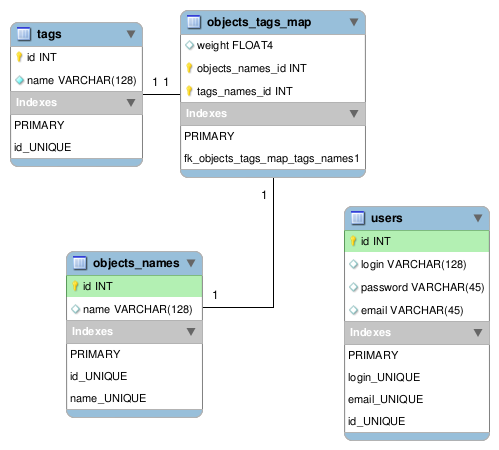
\includegraphics[width=7in,height=8in]{pics/db-scheme-core.png}
\end{center}
\end{figure}

Для работы ядра необходимы следующие таблицы в базе данных:
\begin{itemize}
\item $users$ --- таблица, в которой хранится информация о пользователях. Имеет
	следующую структуру:
  \begin{itemize}
    \item $id$ --- первичный ключ таблицы, целое число;
    \item $login$ --- строка, в которой хранится login пользователя;
    \item $password$ --- строка, в которой хранится пароль пользователя;
    \item $email$ --- строка, в которой хранится email пользователя;
  \end{itemize}
\item $obects\_names$ --- таблица, в которой хранится информация об объектах (objects) предметной области. Имеет следующую структуру:
  \begin{itemize}
    \item $id$ --- первичный ключ таблицы, целое число;
    \item $name$ --- строка, в которой хранится наименование объекта;
  \end{itemize}
\item $tags$  --- таблица, в которой хранится информация о тегах
	предметной области. Теги --- популярный термин, который несет семантику характеристики. Имеет следующую структуру:
  \begin{itemize}
    \item $id$ - первичный ключ таблицы, целое число;
    \item $name$ --- строка, в которой хранится наименование объекта;
  \end{itemize}
\item $objects\_tags\_map$ --- таблица, в которой хранится информация о характеристиках объектов. Имеет следующую структуру:
  \begin{itemize}
    \item $oid$ --- внешний ключ таблицы, связанный с $id$ таблицы $obects\_names$;
    \item $tid$ --- внешний ключ таблицы, связанный с $id$ таблицы $tags$;
    \item $(oid, tid)$ --- пара внешних ключей составляет первичный ключ таблицы;
    \item $weight$ --- вещественное число, являющееся значением характеристики или весом тега;
  \end{itemize}
\end{itemize}

\section{Описание ядра системы}
Ядро системы написано на языке Java с применением технологии Java Servlet-ов,
для использования которых был развернут контейнер сервлетов --- сервер
Apache Tomcat, который позволяет запускать веб-приложения.

Программное обеспечение обладает архитектурой пакетов, изображенной на
UML-диаграммах (\ref{entres-uml1}) и (\ref{entres-uml2}).
\begin{figure}[h]
\caption{UML-диаграмма пакетов ядра}
	\label{entres-uml1}
\begin{center}
  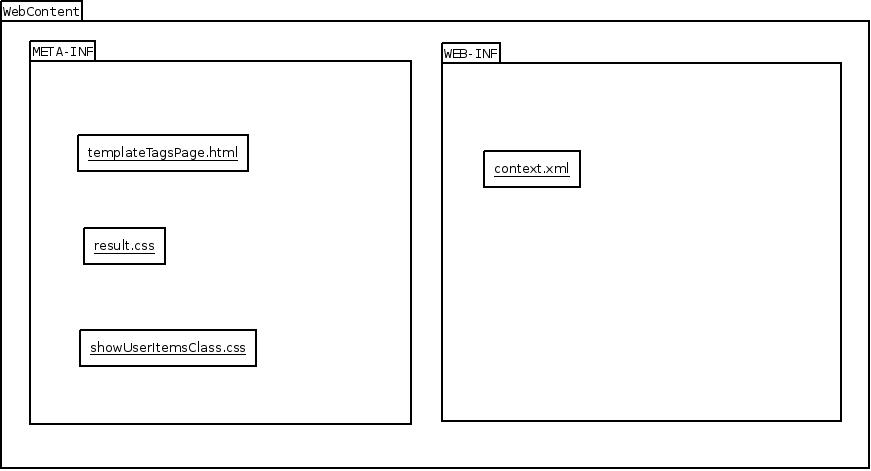
\includegraphics[width=7in,height=7in]{pics/core-web-content.jpeg}
\end{center}
\end{figure}
В Web пакеты ядра входят следующие составляющие:
\begin{enumerate}
\item Пакет <<WEB-INF>>, в котором определены <<.js>> скрипты, стилевые файлы и
	файл-шаблон для предварительных действий, проводимых перед запуском
		системы;
\item Пакет <<META-INF>> содержит файл <<context.xml>>,
	в котором описывается контекст подключения к базе данных.
\end{enumerate}

\begin{figure}
\caption{UML-диаграмма пакетов ядра.}
\label{entres-uml2}
\begin{center}
  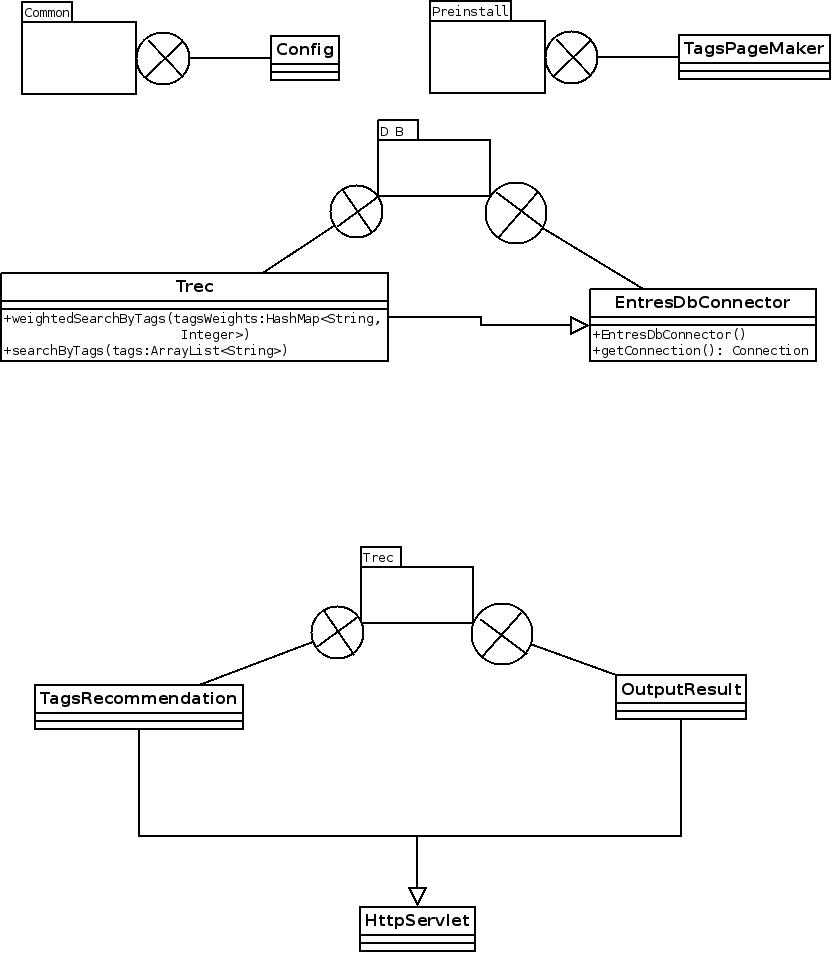
\includegraphics[width=7in,height=10in]{pics/core-packs2.jpeg}
\end{center}
\end{figure}

Ядро системы состоит из следующих пакетов и классов:
\begin{itemize}
	\item Common --- пакет, содержащий общие для всего ядра элементы:
		\begin{itemize}
			\item Класс <<Config>> --- в нем пользователь ядра должен задать
				конфигурационные константы своего приложения, такие, например, как,
				имена таблиц базы данных.
		\end{itemize}
	\item Пакет <<Preinstall>> --- данный пакет содержит классы,
		которые выполняют предварительные действия, необходимые для запуска
		приложения;
	\item <<TagsPageMaker>> --- класс, с помощью которого формируется
		html-страницы веб-сервиса с конcтантным
		  именем <<tagsInputPage.html>>, на которой
		  пользователь может задать теги для поиска интересующих объектов.
		  Страница <<tagsInputPage.html>> формируется по шаблону,
		  входящему в ядро системы --- в пакете WEB-INF,
		  файл <<templateTagsPage.html>>. Это необходимое предварительное
		  действие, необходимое для запуска сервиса, так как ядро не имеет
		  никакой информации о конкретной базе, с которой придется работать.
		  При желании изменения стиля сформированной страницы пользователь ядра
		  может изменить стилевой файл/
	  \item Пакет DB (от Data Base) --- содержит классы, которые осуществляют
		  работу с базой данных. В данном пакете определены следующие классы:
		  \begin{itemize}
			  \item Базовый класс <<EntresDbConnector>>, который описывает
				  подключение к бае данных.
			  \item Класс <<Trec (от Tag Recommendation)>>, наследуемый от
				  класс <<EntresDbConnector>>. В нем определены функции, необходимые ядру
				  для осуществления поиска объектов по заданным тегам. С данным классом осуществляют работу Java-сервлеты после получения данных от пользователя.
				  Класс содержит основные публичные методы:
				  \begin{itemize}
					  \item <<weightedSearchByTags>> --- поиск по тегам,
						  заданных пользователем вместе с указанием их веса;
					  \item <<searchByTags>> --- поиск объектов по списку
						  тегов, заданных пользователем.
				  \end{itemize}
		  \end{itemize}
	  \item <<Trec>> --- данный пакет содержит сервлеты, которые в
		  иерархически
		  находятся между пользователем и базой данных.
		  В пакет входят следующие сервлеты:
		  \begin{itemize}
			  \item <<TagsRecommendation>> --- сервлет, получающий информацию от пользователя и делающий запрос в базу данных
				  на поиск соответствующих объектов через класс Trec пакета DB;
			  \item <<OutputResult>> --- сервлет получающий управление после форвардинга из сервлета <<TagsRecommendation>>. Данный сервлет осуществляет
				  вывод результатов поиска по базе на веб-страницу;
		  \end{itemize}
\end{itemize}

\section{Описание рекомендательного кинематографического веб-сервиса}
На базе ядра было разработано приложение для кинематографиских рекомендаций.
В качестве таблицы $objects\_tags\_map$ использовались данные базы Movie Lens.
В сформированной базе на основе Movie Lens содержится 30 000 фильмов и 200 жанров.
Характеристики объектов могут принимать значения 0 либо 1, в зависимости от того,
принадлежит ли жанр объекту или нет (то есть $w(i, y) \in \{0,1\}$).
В действительности число жанров гораздо больше, но в создаваемом приложении огромное число 
жанров затруднит формирование запроса. Характеристики пользователя совпадают с
характеристиками объекта, то есть $\delta_c(x, y) = 1$.

Помимо основной функциональности была добавлена возможность сохранения пользователем
интересующих его фильмов и просмотр текущего списка. Для этого к базе была
добавлена
дополнительная таблица, что отражено в UML-диаграмме (\ref{pic:db-ml}).

\begin{figure}
\caption{Структура базы данных кинематографического сервиса}
\label{pic:db-ml}
\begin{center}
  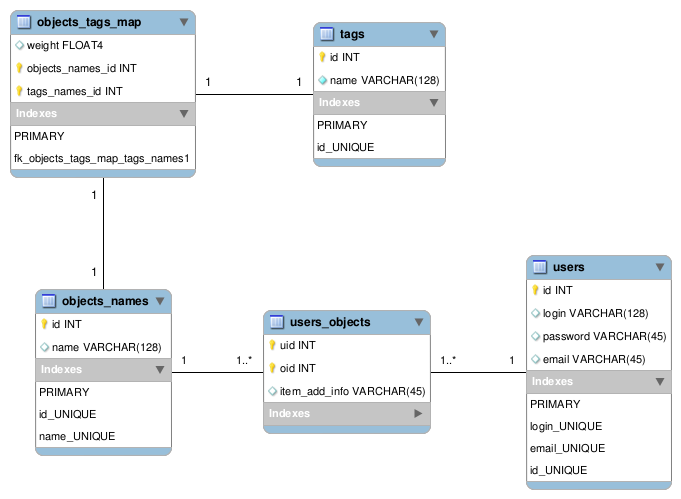
\includegraphics[width=7in,height=6in]{pics/db-scheme-ml.png}
\end{center}
\end{figure}

База содержит дополнительную таблицу $users\_objects$ со следующей структурой:
\begin{itemize}
\item $uid$ --- внешний ключ таблицы, связанный с $id$ таблицы $users$;
\item $oid$ --- внешний ключ таблицы, связанный с $id$ таблицы $obects\_names$;
\item $(uid, oid)$ --- пара внешних ключей составляет первичный ключ таблицы;
\item $item\_add\_info$ --- дополнительная информация, известная о фильме, хранимая в виде строки;
\end{itemize}

Для отображения пользовательской информации был добавлен класс <<ShowUserInfo
>> в пакет Trec, что изображено на следующей UML-диаграмме.
\begin{figure}
\caption{UML-диаграмма пакетов ядра.}
\begin{center}
  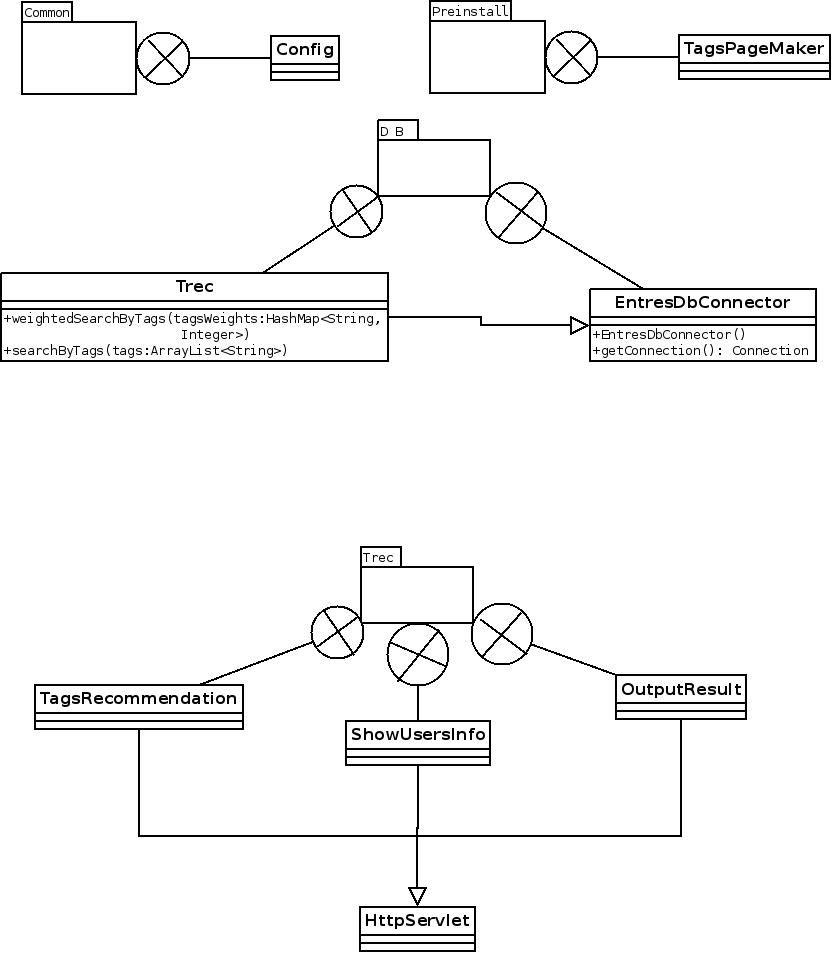
\includegraphics[width=7in,height=7in]{pics/core-packs-ml.jpeg}
\end{center}
\end{figure}

Приведем пример работы с веб-приложением с помощью нескольких скриншотов системы.
На первом скриншоте (\ref{pic:ml-screen1}) виден основной интерфейс пользователя, с помощью которого
он может выбрать интересующие его кинематографические жанры.
\begin{figure}
\caption{Пример выбора пользователем кинематографических жанров для поиска соответствующих им фильмов.}
\label{pic:ml-screen1}
\begin{center}
  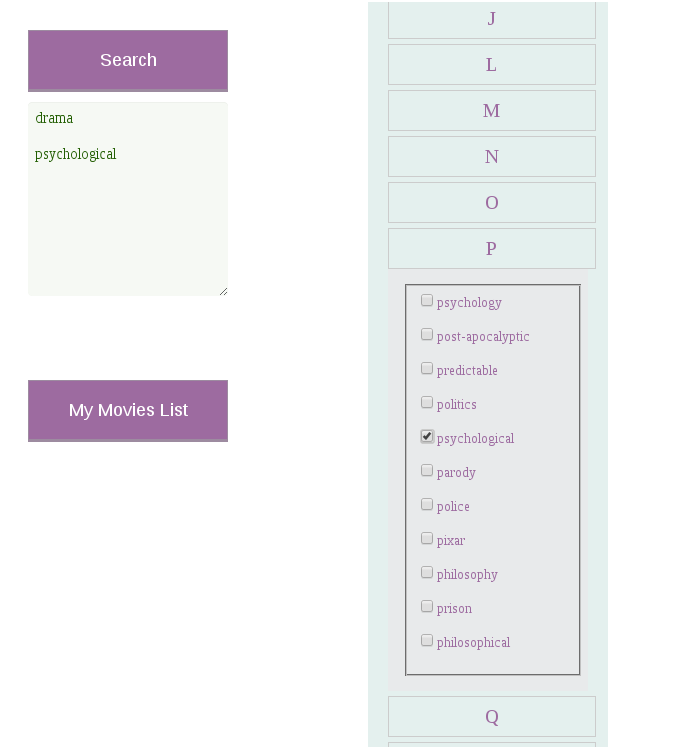
\includegraphics[width=8in,height=9in]{pics/ml-interface.png}
\end{center}
\end{figure}

При задании жанров пользователь формирует собственный контент, значения характеристик принадлежат шкале $\{0,1\}$.
0 --- если пользователь не выбрал жанр, 1 --- иначе. Задача заключается в поиске топовых объектов, поэтому
из базы данных выбираются те объекты, которым принадлежат все выбранные
пользователем характеристик. Результатом
такой выборки являются такие объекты, что $\rho(u_a, i) = 0$.

На скриншоте виден выбор пользователя: его интересуют фильмы, которые обладают
жанрами
<<драма>> и <<психологический>>. На этом же изображении
видна кнопка <<My movies list>>, по нажатию которой пользователь
сможет просмотреть информацию о фильмах, ранее им сохраненных
(см. Рисунок <<Пример списка сохраненных ранее пользователем фильмов>> \ref{pics:save}).
%==========================>
\begin{figure}
\caption{Пример списка сохраненных ранее пользователем фильмов}
	\label{pics:save}
\begin{center}
  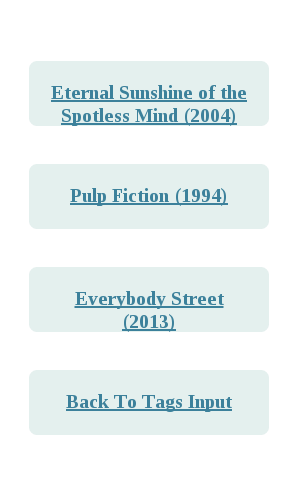
\includegraphics[width=5in,height=5in]{pics/ml-mylist.png}
\end{center}
\end{figure}

На следующем скриншоте (\ref{pic:ml-screen2}) показаны результаты поиска фильмов по запросу пользователя. Если запрос пользователя не устраивает, то
можно сделать повторный и получить другие результаты, нажав кнопку <<Reload>>. Под каждым названием пользователь может
установить галочку и нажать кнопку <<Save Result>>, чтобы занести интересующий его фильм в собственный список.
Так же выводится дополнительная информация о фильме --- IMDB рейтинг. Данная информация сохраняется в колонку  $item\_add\_info$
таблицы $users\_objects$.
\begin{figure}
\caption{Пример результата поиска фильмов}
\label{pic:ml-screen2}
\begin{center}
  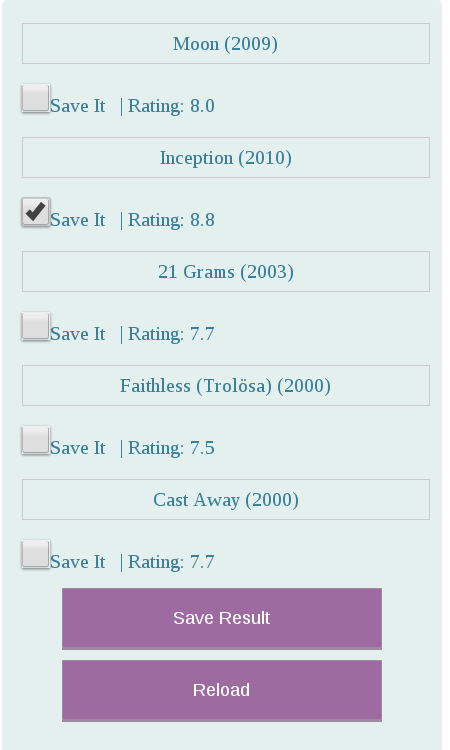
\includegraphics[width=5in,height=5in]{pics/ml-rslt.png}
\end{center}
\end{figure}

\section{Описание рекомендательного музыкального веб-сервиса}
На базе ядра был разработан веб-сервис для поиска музыкальных исполнителей
по заданным пользователям музыкальным жанрам. Музыкальные жанры были
взяты с помощью Last Fm API и среди всего их большого множества оставлены
наиболее
популярные. Всего в базе хранится больше полумиллиона объектов и около 200
самых
распространенных музыкальных жанров. Характеристики пользователя совпадают с
характеристикми объекта.

Созданный веб-сервис имеет дополнительную функциональность, добавленную к ядру:
\begin{itemize}
\item Ведется история выборов пользователей: для этого добавлена таблица $users\_tags$;
\item Существует возможность прослушать понравившееся произведения, отмеченные
	таковыми пользователем ранее. Для этого
добавлена таблица $users\_objects$ и реализован класс <<ShowUserInfo>> в пакете
		<<Trec>>;
\item Вывод результатов сформирован так, что пользователь тут же может
	прослушать найденных исполнителей.
Для этого производится запрос видео на <<Youtube>>, для чего создан класс запроса
		расширенной информации об объекте
<<ExtendedAdditionalQuery>>, входящий в состав пакета <<Trec>>;
\end{itemize}

На следующей UML-диаграмме (\ref{pic:db-lf}) отображена структура базы сервиса.

\begin{figure}
\caption{Структура базы данных рекомендательного музыкального веб-сервиса.}
\label{pic:db-lf}
\begin{center}
  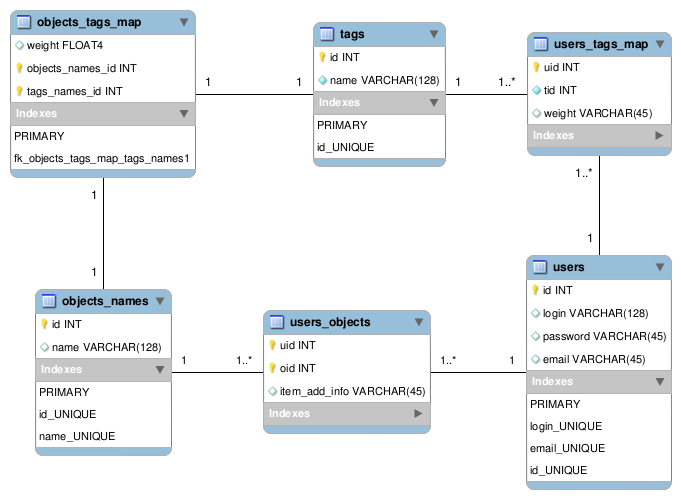
\includegraphics[width=7in,height=6in]{pics/db-scheme-lastfm.png}
\end{center}
\end{figure}

База содержит дополнительную таблицу $users\_tags$ со следующей структурой:
\begin{itemize}
\item $uid$ --- внешний ключ таблицы, связанный с $id$ таблицы $users$;
\item $tid$ --- внешний ключ таблицы, связанный с $id$ таблицы $tags$;
\item $(uid, tid)$ --- пара внешних ключей составляет первичный ключ таблицы;
\end{itemize}

Структура пакетов отображена на следующей UML-диаграмме (\ref{pic:lf-packs}).
\begin{figure}
\caption{UML-диаграмма пакетов ядра}
\label{pic:lf-packs}
\begin{center}
  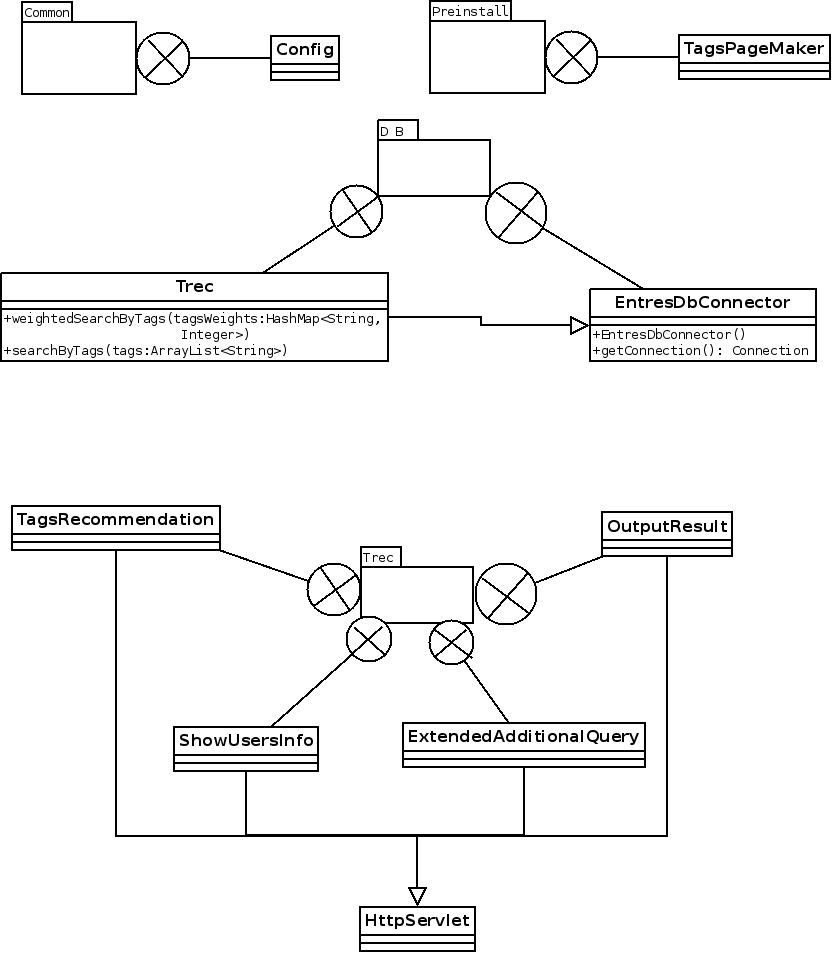
\includegraphics[width=5in,height=5in]{pics/core-packs-lastfm.jpeg}
\end{center}
\end{figure}

Приведем пример работы с веб-приложением с помощью нескольких скриншотов системы.
На первом скриншоте виден основной интерфейс пользователя, с помощью которого
он может выбрать интересующие его кинематографические жанры. Разработанный веб-сервис
имеет более расширенную версию выбора жанров по сравнению с предыдущим сервисом:
пользователь может указать <<вес>> жанра. В терминах нечеткой модели данный вес
отображает степень принадлежности жанра контенту пользователя, который он формирует
при составлении запроса. То есть $w(u,x) \in \{0; 0,3; 0,6; 1\}$. Семантическое соответствие:
\begin{itemize}
\item 0 --- жанр не выбран;
\item 0,3 --- низкая принадлежность;
\item 0,6 --- средняя принадлежность;
\item 1 --- высокая принадлежность.
\end{itemize}
Отображение контета пользователя на множества контентов объектов является тождественным, так как $X = Y$,
но с учетом табицы соответствия значений характеристик пользователя характеристикам объекта $delta_c$:
\begin{table}[h]
\caption{Таблица соответствия характеристик пользователей характеристикам объектов}
\begin{tabular}{|c|c|}
  \hline
  Значение характеристики пользователя & Интервал значений характеристики объекта \\ \hline
  0   & [0; 0,]) \\ \hline
  0,3 &  (0,5; 0,4] \\ \hline
  0,6 & (0,4; 0,7] \\ \hline
  1 & (0,7; 1] \\ \hline
\end{tabular}
\end{table}
К примеру, пользователю с контентом \{(<<Blues>>; 0,8)\} будет
соответствовать объекты, которым принадлежат пары \{(<<blues>>; n)\}, где
$n \in [0,1]$. К примеру, по данному запросу пользователь может получить объект
с именем \{(<<B. B. King>>\}. Таким образом, выбираются объекты,
для которых $\rho(u_a, i) < 0,3$.


На скриншоте (\ref{pic:lf-screen1}) виден выбор пользователя: его интересуют музыкальные исполнители, для которых жанр <<blues>> имеет
высокую принадлежность и жанр <<rock>> --- среднюю.
\begin{figure}[h]
\caption{Пример выбора пользователем музыкальных жанров для поиска соответствующих им исполнителей.}
\label{pic:lf-screen1}
\begin{center}
  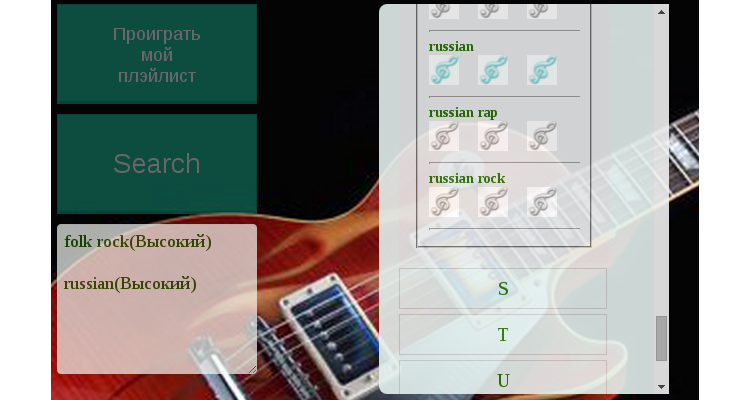
\includegraphics[width=5in,height=3in]{pics/lastfm-interface.png}
\end{center}
\end{figure}

На следующем скриншоте (\ref{pic:lf-screen2}) изображен результат запроса.
\begin{figure}[h]
\caption{Пример результата запроса на поиск музыкальных исполнителей.}
\label{pic:lf-screen2}
\begin{center}
  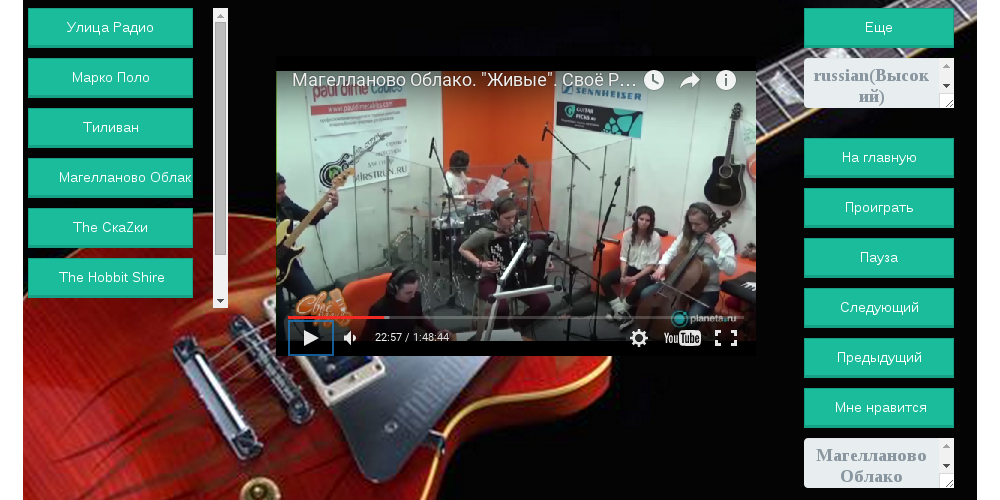
\includegraphics[width=5in,height=3in]{pics/lastfm-rslt.png}
\end{center}
\end{figure}

На скриншоте (\ref{pic:lf-screen2}) видна дополнительная, по сравнению с
предыдущим сервисом, функциональность: можно прослушивать и просматривать
видео исполнителей, выбирая их с помощью навигационных кнопок и сохранять понравившихся в свой плэйлст.

На последнем рисунке <<Пример paylist-a пользователя>> (\ref{pic:lf-screen4}) изображен paylist пользователя. Здесь он может прослушивать понравившиеся и сохраненные ранее им исполнители.
\begin{figure}[h]
\caption{Пример paylist-a пользователя}
\label{pic:lf-screen4}
\begin{center}
  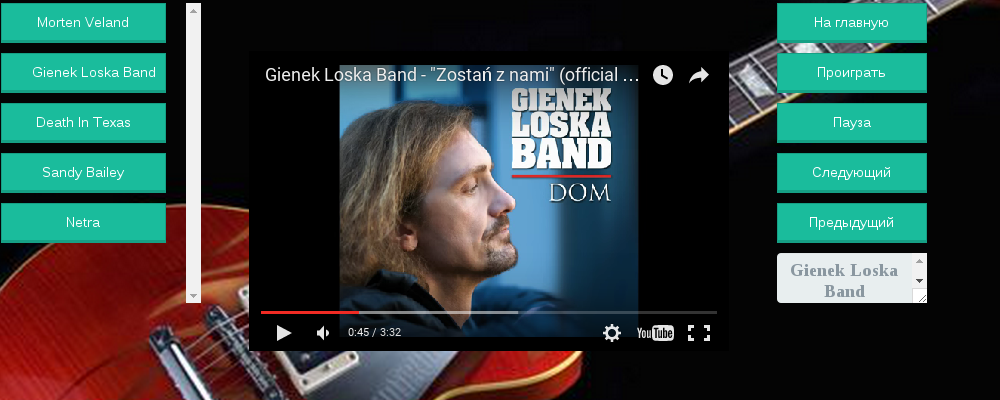
\includegraphics[width=5in,height=3in]{pics/lastfm-mylist.png}
\end{center}
\end{figure}

           % Глава 3
\chapter*{Заключение}						% Заголовок
\addcontentsline{toc}{chapter}{Заключение}	% Добавляем его в оглавление

%% Согласно ГОСТ Р 7.0.11-2011:
%% 5.3.3 В заключении диссертации излагают итоги выполненного исследования, рекомендации, перспективы дальнейшей разработки темы.
%% 9.2.3 В заключении автореферата диссертации излагают итоги данного исследования, рекомендации и перспективы дальнейшей разработки темы.
%% Поэтому имеет смысл сделать эту часть общей и загрузить из одного файла в автореферат и в диссертацию:
В рамках проведенного диссертационного исследования решена актуальная
научно-техническая задача построения математической модели рекомендательной
системы. Теоретически и практически показано, что разработанная модель
является эффективным расширением существующей
анамнестической коллаборативной модели.

В ходе диссертационного исследования были решены все поставленные
цели и задачи:

\begin{enumerate}
	\item
		проведен анализ эффективности АКМ по критериям оценки
		эффективности моделей РС. Показано, что в общем случае
		анамнестическая коллаборативная модель не является
		эффективной моделью рекомендательной системы;
	\item разработана модель рекомендательной системы на нечетких
		множествах и алгоритмы решений задач в рамках этой модели.
		Показано, что разработанная модель является эффективным расширением
		анамнестической коллаборативной модели;
	\item разработано программное обеспечение, с помощью которого
		было проведено тестирование разработанной и анамнестической
		коллаборативной моделей. Результаты тестирования подтверждают
		теоретический вывод о том, что разработанная модель более эффективна,
		чем анамнестическая коллаборативная модель.
\end{enumerate}
      % Заключение
\chapter*{Список сокращений и условных обозначений}             % Заголовок
\addcontentsline{toc}{chapter}{Список сокращений и условных обозначений}  % Добавляем его в оглавление
\noindent
\addtocounter{table}{-1}% Нужно откатить на единицу счетчик номеров таблиц, так как следующая таблица сделана для удобства представления информации по ГОСТ
%\begin{longtabu} to \dimexpr \textwidth-5\tabcolsep {r X}
	\begin{longtable}{p{3cm}p{13cm}}
	$\rho$ & оценка близости пользователя и объекта\\
	$\Delta_{\R}$ & пороговое значение оценки близости $\rho$, по которому
	устанавливается выполнение отношения близости\\
		$\Delta_{u}$ & пороговое значение меры сходства $\du$, по которому
	устанавливается выполнение отношения близости $\ru$\\
		$\Delta_{i}$ & пороговое значение меры сходства $\di$, по которому
	устанавливается выполнение отношения близости $\rt$\\
	$I$ & множество объектов \\
	$U$ & множество пользователей \\
	$i$ & объект \\
	$i_0$ & объект, принадлежащий обучающему множеству \\
	$i_{\bot}$ & объект, принадлежащий тестовому множеству. Также
	прогнозируемый объект. \\
	$u$ & пользователь \\
	$t$ & задача\\
	$\overline{P}^a_{\bot}$ & результирующее множество \\
	$task$ & множество задач\\
	$u_a$ & активный пользователь \\
	$p$ & задача прогнозирования \\
	$topN$ & задача $topN$ \\
	$\mathbb{N}$ & множество натуральных чисел\\
	$\varepsilon_p$ & пороговое значение малой величины разницы между оценками
	близости или оценкой близости и значением прогнозной функции
	\\
	$\R$ & отношение близости пользователя и объекта \\
	$P$ & множество исходных данных, которое содержит все известные значения оценки близости \\
	$P_0$ & обучающее множество \\
	$P_{\bot}$ & тестовое множество \\
	$\mathcal{M}_{\rho}$ & матрица значений оценки близости\\
	$\bot$ & неизвестное значение\\
	$w_U$ & весовая функция, сопоставляющая характеристике пользователя вес\\
	$w_I$ & весовая функция, сопоставляющая характеристике объекта вес\\
	$\mathcal{S})_I$ & шкала значений весов характеристик объектов\\
	$\mathcal{S})_U$ & шкала значений весов характеристик пользователей\\
	$X$ & множество всех возможных характеристик пользователей \\
	$Y$ & множество всех возможных характеристик объектов \\
	ООМ & Объектно-ориентированныя модель \\
	СОМ & Субъектно-ориентированныя модель \\
	$I_{topN}$ & множество, содержащее объекты, по алгоритмическому
	выводу РС между которыми и активным пользователем выполняется отношение
	близости. Данное множество формируется в процессе решения задачи $topN$ \\
	$\rh$ & прогнозная функция \\
	$s$ & функция, сопоставляющая объекту 1, если между ним и активным
	пользователем выполняется отношение близости, 0 --- иначе. Применяется при вычислении
	целевой оценки точности\\
	$\overline{s}$ & функция, сопоставляющая объекту 1, если между ним и активным
	пользователем выполняется отношение близости по правилам вывода ООМ,
	0 --- иначе. Применяется при вычислении объектно-ориентированной оценки точности\\
	$|S|$ & мощность некоторого множества $S$\\
	$\eat$ & обобщенная целевая оценка точности \\
	$\eit$ & обобщенная объектно-ориентированная оценка точности \\
	$I^a_0$ & $\{i_0: (i | \rho(u_a, i_0)) \in P_0$ \\
	$\nit$ & кластер соседей-объектов, составляемый при решении задачи $topN$ в
	ООМ\\
	$\nip$ & кластер соседей-объектов, составляемый при решении задачи $p$ в
	ООМ\\
	$\nut$ & кластер соседей-объектов, составляемый при решении задачи $topN$ в
	СОМ\\
	$\nup$ & кластер соседей-объектов, составляемый при решении задачи $p$ в
	СОМ\\
	$\Pi$ & правило алгоритмического вывода значения прогнозной функции\\
	$\Pi_O$ & правило алгоритмического вывода значения прогнозной функции ООМ\\
	$\Pi_C$ & правило алгоритмического вывода значения прогнозной функции СОМ\\
	$\Pi_f$ & правило алгоритмического вывода значения прогнозной функции
	нечеткой модели\\
	$f_p$ & функция, выражающая зависимость между значением прогнозной функции
	и значениями оценок близости пользователей, вошедших в кластер $\nup$ю\\
	$s(i)$ & функция, принимающая значение, равное 1, если $u_a \R
	i, i \in I_{topN}, 0$ --- иначе. Применяется для расчета $\eat$.\\
	$\overline{s}(i)$ & функция, принимающая значение, равное 1,
	если $\exists i_{\bot}: i_{\bot} \rt i, i \in I_{topN}, 0$ --- иначе.
	Применяется для расчета $\eit$.\\
\end{longtable}
        % Список сокращений и условных обозначений
\chapter*{Словарь терминов}             % Заголовок
\addcontentsline{toc}{chapter}{Словарь терминов}  % Добавляем его в оглавление

\textbf{Агент} --- пользователь или объект системы.

\textbf{Эффективность} --- оценочная характеристика РС.

\textbf{Объект} --- некоторая сущность предметной области РС.

\textbf{Пользователь} --- пользователь РС.

\textbf{Характеристика агента} --- единица метаданных агента. Например, жанр
объекта для кинематографической системы.

\textbf{Контент агента} --- структура данных, представляющая информацию об
агенте. Например, вектор.

\textbf{Рекомендательная система} --- программное обеспечение,
функциональность которых заключается в определении информации, которая
будет полезна пользователю.

\textbf{Модель рекомендательная система} --- математическая модель
рекомендательной системы, которая описывает способы представления информации
о пользователях и объектах, методы решения задач и взаимосвязи этой информации.

\textbf{Двумерная модель рекомендательная система} ---
наиболее распространенная модель, получившая свое название от определения
способа взаимосвязи информации о пользователе и объекте, которая
заключается в определении двумерной функции $\rho: U \times I \Rightarrow [0,1]$.

\textbf{Функция близости} --- функция $\rho: U \times I \Rightarrow [0,1]$,
значения которой определяют степень полезности, предпочтения и т.п. объекта
пользователю.

\textbf{Отношение близости пользователя и объекта} --- отношение, которое
формализует такие неформальные понятия как <<пользователю нравится объект>>,
<<объект полезен для пользователя>> и т.п. Факт выполнения отношения
устанавливается по значениям функции близости.

\textbf{Мера сходства пользователей} --- функция $\du: U \times U \Rightarrow
[0,1]$, определяющая степень близости пользователей по их характеристикам.

\textbf{Мера сходства объектов} --- функция $\di: I \times I \Rightarrow
[0,1]$, определяющая степень близости объектов по их характеристикам.

\textbf{Отношение близости объектов} --- отношение, которое определяет
близость агентов системы, определяемую по значениям меры сходства.

\textbf{Активный пользователь} --- пользователь системы, обозначающийся
символом $u_a$, для которого в данный момент решается задача.

\textbf{Задача topN} --- задача, целью которой является формирование
подмножества объектов, между которыми и активным пользователем выполняется
отношение близости.

\textbf{Задача прогнозирования} --- задача, обозначающаяся символом $p$ и
заключающаяся в определении неизвестного значения $\rho(u_a, i)$.

\textbf{Оценка качества} --- функция $\mathcal{E}_t$ оценки качества решения
задачи $t \in \{topn, p\}$.

      % Словарь терминов
%\clearpage                                  % В том числе гарантирует, что список литературы в оглавлении будет с правильным номером страницы
%\hypersetup{ urlcolor=black }               % Ссылки делаем чёрными
%\providecommand*{\BibDash}{}                % В стилях ugost2008 отключаем использование тире как разделителя 
\urlstyle{rm}                               % ссылки URL обычным шрифтом
\ifdefmacro{\microtypesetup}{\microtypesetup{protrusion=false}}{} % не рекомендуется применять пакет микротипографики к автоматически генерируемому списку литературы
\insertbibliofull                           % Подключаем Bib-базы
\ifdefmacro{\microtypesetup}{\microtypesetup{protrusion=true}}{}
\urlstyle{tt}                               % возвращаем установки шрифта ссылок URL
%\hypersetup{ urlcolor={urlcolor} }          % Восстанавливаем цвет ссылок      % Список литературы
%\clearpage
%\listoffigures  % Список изображений
%\ifdefmacro{\microtypesetup}{\microtypesetup{protrusion=false}}{} % не рекомендуется применять пакет микротипографики к автоматически генерируемым спискам

%%% Список таблиц %%%
% (ГОСТ Р 7.0.11-2011, 5.3.10)
\clearpage
\listoftables   % Список таблиц
\ifdefmacro{\microtypesetup}{\microtypesetup{protrusion=true}}{}
           % Списки таблиц и изображений (иллюстративный материал)
\appendix
%%% Оформление заголовков приложений ближе к ГОСТ:
\setlength{\midchapskip}{20pt}
\renewcommand*{\afterchapternum}{\par\nobreak\vskip \midchapskip}
\renewcommand\thechapter{\Asbuk{chapter}} % Чтобы приложения русскими буквами нумеровались
   % Предварительные настройки для правильного подключения Приложений
%%\chapter{Примеры вставки листингов программного кода} \label{AppendixA}
%%
%%Для крупных листингов есть два способа. Первый красивый, но в нём могут быть проблемы с поддержкой кириллицы (у вас может встречаться в комментариях и
%%печатаемых сообщениях), он представлен на листинге~\ref{list:hwbeauty}.
%%\begin{ListingEnv}[!h]% настройки floating аналогичны окружению figure
%%%    \captionsetup{format=tablenocaption}% должен стоять до самого caption
%%    \caption{Программа “Hello, world” на \protect\cpp}
%%    % далее метка для ссылки:
%%    \label{list:hwbeauty}
%%    % окружение учитывает пробелы и табуляции и применяет их в сответсвии с настройками
%%    \begin{lstlisting}[language={[ISO]C++}]
%%	#include <iostream>
%%	using namespace std;
%%
%%	int main() //кириллица в комментариях при xelatex и lualatex имеет проблемы с пробелами
%%	{
%%		cout << "Hello, world" << endl; //latin letters in commentaries
%%		system("pause");
%%		return 0;
%%	}
%%    \end{lstlisting}
%%\end{ListingEnv}%
%%Второй не такой красивый, но без ограничений (см.~листинг~\ref{list:hwplain}).
%%\begin{ListingEnv}[!h]
%%    \caption{Программа “Hello, world” без подсветки}
%%    \label{list:hwplain}
%%    \begin{Verb}
%%        
%%        #include <iostream>
%%        using namespace std;
%%        
%%        int main() //кириллица в комментариях
%%        {
%%            cout << "Привет, мир" << endl;
%%        }
%%    \end{Verb}
%%\end{ListingEnv}
%%
%%Можно использовать первый для вставки небольших фрагментов
%%внутри текста, а второй для вставки полного
%%кода в приложении, если таковое имеется.
%%
%%Если нужно вставить совсем короткий пример кода (одна или две строки), то выделение  линейками и нумерация может смотреться чересчур громоздко. В таких случаях можно использовать окружения \texttt{lstlisting} или \texttt{Verb} без \texttt{ListingEnv}. Приведём такой пример с указанием языка программирования, отличного от заданного по умолчанию:
%%\begin{lstlisting}[language=Haskell]
%%fibs = 0 : 1 : zipWith (+) fibs (tail fibs)
%%\end{lstlisting}
%%Такое решение~--- со вставкой нумерованных листингов покрупнее
%%и вставок без выделения для маленьких фрагментов~--- выбрано,
%%например, в книге Эндрю Таненбаума и Тодда Остина по архитектуре
%%%компьютера~\autocite{TanAus2013} (см.~рис.~\ref{fig:tan-aus}).
%%
%%Наконец, для оформления идентификаторов внутри строк
%%(функция \lstinline{main} и тому подобное) используется
%%\texttt{lstinline} или, самое простое, моноширинный текст
%%(\texttt{\textbackslash texttt}).
%%
%%
%%Пример~\ref{list:internal3}, иллюстрирующий подключение переопределённого языка. Может быть полезным, если подсветка кода работает криво. Без дополнительного окружения, с подписью и ссылкой, реализованной встроенным средством.
%%\begin{lstlisting}[language={Renhanced},caption={Пример листинга c подписью собственными средствами},label={list:internal3}]
%%## Caching the Inverse of a Matrix
%%
%%## Matrix inversion is usually a costly computation and there may be some
%%## benefit to caching the inverse of a matrix rather than compute it repeatedly
%%## This is a pair of functions that cache the inverse of a matrix.
%%
%%## makeCacheMatrix creates a special "matrix" object that can cache its inverse
%%
%%makeCacheMatrix <- function(x = matrix()) {#кириллица в комментариях при xelatex и lualatex имеет проблемы с пробелами
%%    i <- NULL
%%    set <- function(y) {
%%        x <<- y
%%        i <<- NULL
%%    }
%%    get <- function() x
%%    setSolved <- function(solve) i <<- solve
%%    getSolved <- function() i
%%    list(set = set, get = get,
%%    setSolved = setSolved,
%%    getSolved = getSolved)
%%    
%%}
%%
%%
%%## cacheSolve computes the inverse of the special "matrix" returned by
%%## makeCacheMatrix above. If the inverse has already been calculated (and the
%%## matrix has not changed), then the cachesolve should retrieve the inverse from
%%## the cache.
%%
%%cacheSolve <- function(x, ...) {
%%    ## Return a matrix that is the inverse of 'x'
%%    i <- x$getSolved()
%%    if(!is.null(i)) {
%%        message("getting cached data")
%%        return(i)
%%    }
%%    data <- x$get()
%%    i <- solve(data, ...)
%%    x$setSolved(i)
%%    i  
%%}
%%\end{lstlisting} %$ %Комментарий для корректной подсветки синтаксиса
%%                 %вне листинга
%%
%%Листинг~\ref{list:external1} подгружается из внешнего файла. Приходится загружать без окружения дополнительного. Иначе по страницам не переносится.
%%    \lstinputlisting[lastline=78,language={R},caption={Листинг из внешнего файла},label={list:external1}]{listings/run_analysis.R}
%%
%%
%%
%%
%%
%%
%
\chapter{Свидетельство о регистрации программного обеспечения}
\begin{figure}[H]
  \begin{center}
  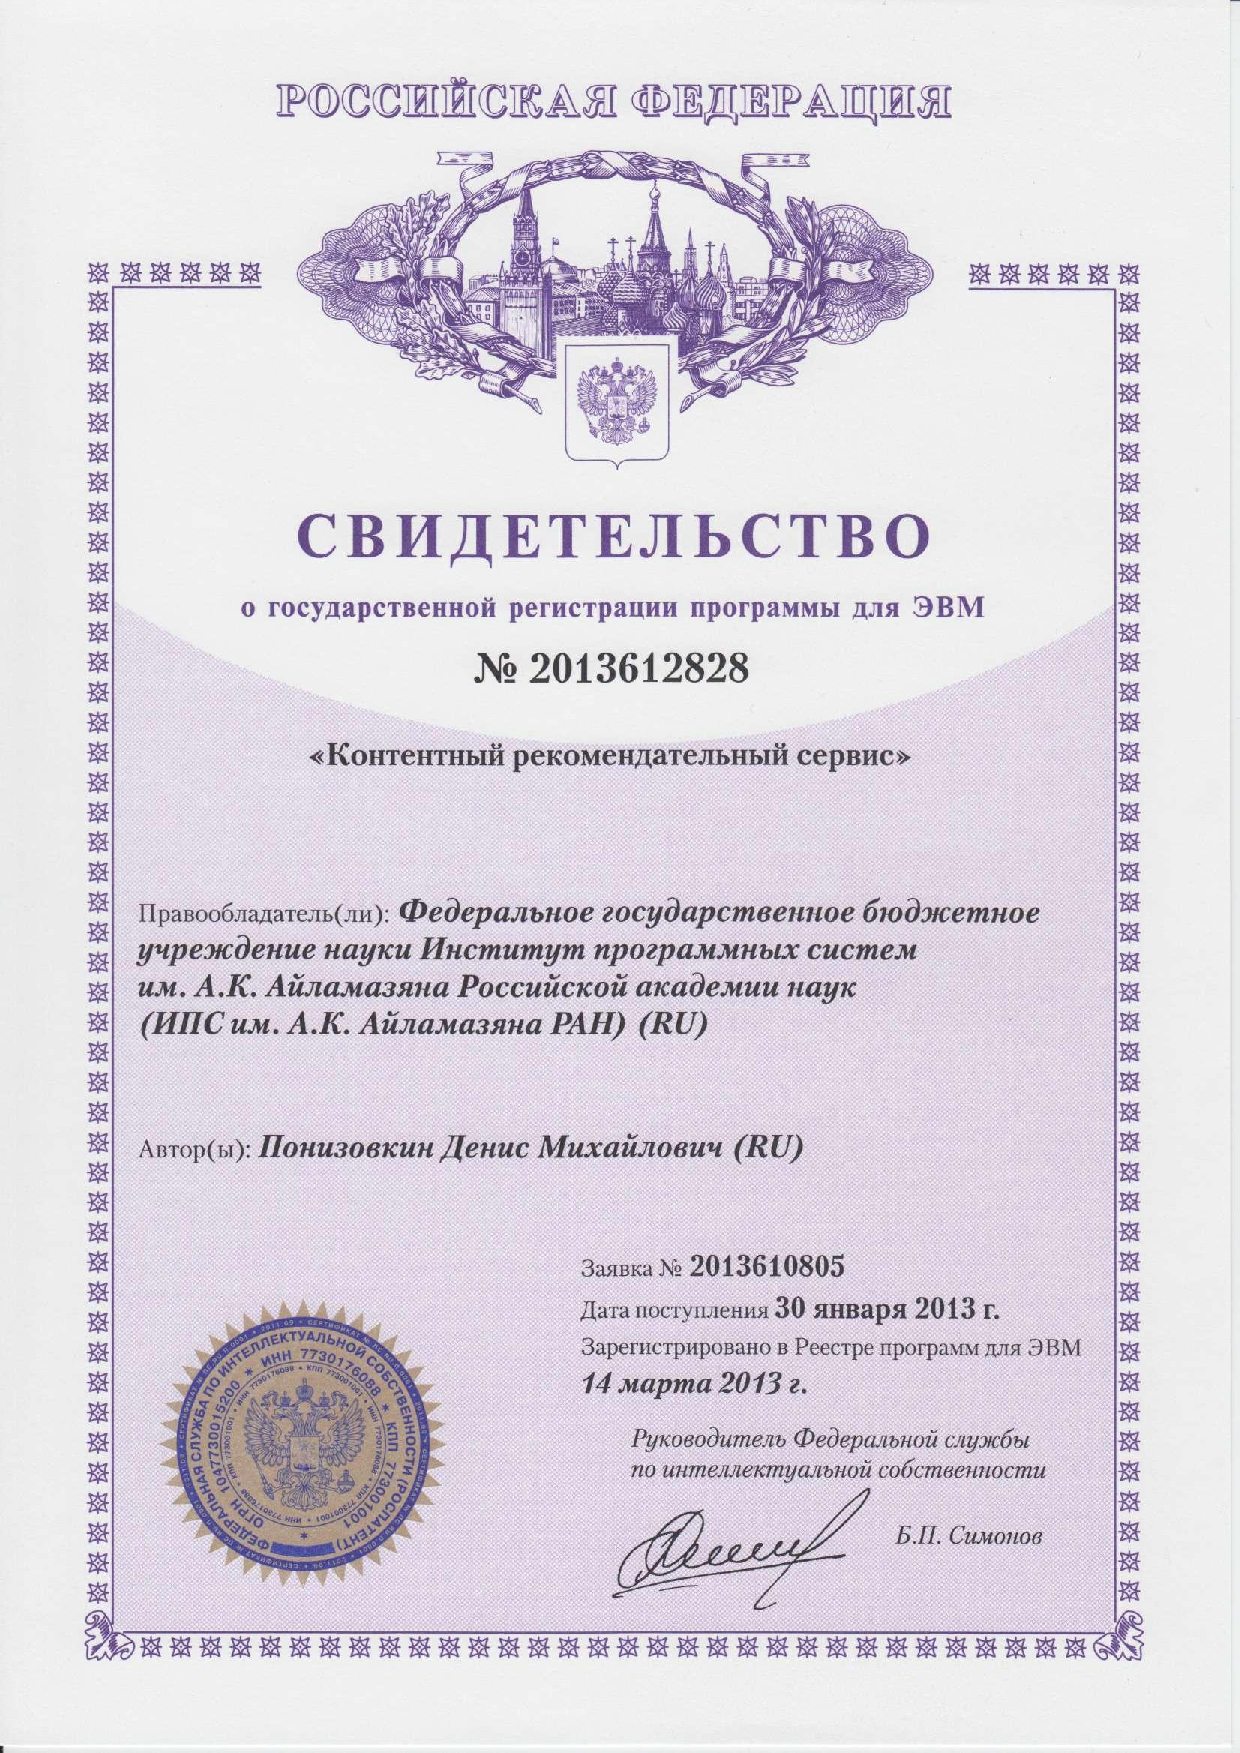
\includegraphics[width=6in,height=6in]{pics/svidetelstvo}
	\end{center}
\end{figure}

\chapter{Акты, подтверждающие внедрение и использование результатов
диссертационной работы}
%%Вот размещается длинная таблица:
%%\fontsize{10pt}{10pt}\selectfont
%%\begin{longtable*}[c]{|l|c|l|l|} %longtable* появляется из пакета caption и даёт ненумерованную таблицу
%%% \caption{Описание входных файлов модели}\label{Namelists} 
%%%\\ 
%% \hline
%% %\multicolumn{4}{|c|}{\textbf{Файл puma\_namelist}}        \\ \hline
%% Параметр & Умолч. & Тип & Описание               \\ \hline
%%                                              \endfirsthead   \hline
%% \multicolumn{4}{|c|}{\small\slshape (продолжение)}        \\ \hline
%% Параметр & Умолч. & Тип & Описание               \\ \hline
%%                                              \endhead        \hline
%%% \multicolumn{4}{|c|}{\small\slshape (окончание)}        \\ \hline
%%% Параметр & Умолч. & Тип & Описание               \\ \hline
%%%                                             \endlasthead        \hline
%% \multicolumn{4}{|r|}{\small\slshape продолжение следует}  \\ \hline
%%                                              \endfoot        \hline
%%                                              \endlastfoot
%% \multicolumn{4}{|l|}{\&INP}        \\ \hline 
%% kick & 1 & int & 0: инициализация без шума ($p_s = const$) \\
%%      &   &     & 1: генерация белого шума                  \\
%%      &   &     & 2: генерация белого шума симметрично относительно \\
%%  & & & экватора    \\
%% mars & 0 & int & 1: инициализация модели для планеты Марс     \\
%% kick & 1 & int & 0: инициализация без шума ($p_s = const$) \\
%%      &   &     & 1: генерация белого шума                  \\
%%      &   &     & 2: генерация белого шума симметрично относительно \\
%%  & & & экватора    \\
%% mars & 0 & int & 1: инициализация модели для планеты Марс     \\
%%kick & 1 & int & 0: инициализация без шума ($p_s = const$) \\
%%      &   &     & 1: генерация белого шума                  \\
%%      &   &     & 2: генерация белого шума симметрично относительно \\
%%  & & & экватора    \\
%% mars & 0 & int & 1: инициализация модели для планеты Марс     \\
%%kick & 1 & int & 0: инициализация без шума ($p_s = const$) \\
%%      &   &     & 1: генерация белого шума                  \\
%%      &   &     & 2: генерация белого шума симметрично относительно \\
%%  & & & экватора    \\
%% mars & 0 & int & 1: инициализация модели для планеты Марс     \\
%%kick & 1 & int & 0: инициализация без шума ($p_s = const$) \\
%%      &   &     & 1: генерация белого шума                  \\
%%      &   &     & 2: генерация белого шума симметрично относительно \\
%%  & & & экватора    \\
%% mars & 0 & int & 1: инициализация модели для планеты Марс     \\
%%kick & 1 & int & 0: инициализация без шума ($p_s = const$) \\
%%      &   &     & 1: генерация белого шума                  \\
%%      &   &     & 2: генерация белого шума симметрично относительно \\
%%  & & & экватора    \\
%% mars & 0 & int & 1: инициализация модели для планеты Марс     \\
%%kick & 1 & int & 0: инициализация без шума ($p_s = const$) \\
%%      &   &     & 1: генерация белого шума                  \\
%%      &   &     & 2: генерация белого шума симметрично относительно \\
%%  & & & экватора    \\
%% mars & 0 & int & 1: инициализация модели для планеты Марс     \\
%%kick & 1 & int & 0: инициализация без шума ($p_s = const$) \\
%%      &   &     & 1: генерация белого шума                  \\
%%      &   &     & 2: генерация белого шума симметрично относительно \\
%%  & & & экватора    \\
%% mars & 0 & int & 1: инициализация модели для планеты Марс     \\
%%kick & 1 & int & 0: инициализация без шума ($p_s = const$) \\
%%      &   &     & 1: генерация белого шума                  \\
%%      &   &     & 2: генерация белого шума симметрично относительно \\
%%  & & & экватора    \\
%% mars & 0 & int & 1: инициализация модели для планеты Марс     \\
%%kick & 1 & int & 0: инициализация без шума ($p_s = const$) \\
%%      &   &     & 1: генерация белого шума                  \\
%%      &   &     & 2: генерация белого шума симметрично относительно \\
%%  & & & экватора    \\
%% mars & 0 & int & 1: инициализация модели для планеты Марс     \\
%%kick & 1 & int & 0: инициализация без шума ($p_s = const$) \\
%%      &   &     & 1: генерация белого шума                  \\
%%      &   &     & 2: генерация белого шума симметрично относительно \\
%%  & & & экватора    \\
%% mars & 0 & int & 1: инициализация модели для планеты Марс     \\
%%kick & 1 & int & 0: инициализация без шума ($p_s = const$) \\
%%      &   &     & 1: генерация белого шума                  \\
%%      &   &     & 2: генерация белого шума симметрично относительно \\
%%  & & & экватора    \\
%% mars & 0 & int & 1: инициализация модели для планеты Марс     \\
%%kick & 1 & int & 0: инициализация без шума ($p_s = const$) \\
%%      &   &     & 1: генерация белого шума                  \\
%%      &   &     & 2: генерация белого шума симметрично относительно \\
%%  & & & экватора    \\
%% mars & 0 & int & 1: инициализация модели для планеты Марс     \\
%%kick & 1 & int & 0: инициализация без шума ($p_s = const$) \\
%%      &   &     & 1: генерация белого шума                  \\
%%      &   &     & 2: генерация белого шума симметрично относительно \\
%%  & & & экватора    \\
%% mars & 0 & int & 1: инициализация модели для планеты Марс     \\
%%kick & 1 & int & 0: инициализация без шума ($p_s = const$) \\
%%      &   &     & 1: генерация белого шума                  \\
%%      &   &     & 2: генерация белого шума симметрично относительно \\
%%  & & & экватора    \\
%% mars & 0 & int & 1: инициализация модели для планеты Марс     \\
%% \hline
%%  %& & & $\:$ \\ 
%% \multicolumn{4}{|l|}{\&SURFPAR}        \\ \hline
%%kick & 1 & int & 0: инициализация без шума ($p_s = const$) \\
%%      &   &     & 1: генерация белого шума                  \\
%%      &   &     & 2: генерация белого шума симметрично относительно \\
%%  & & & экватора    \\
%% mars & 0 & int & 1: инициализация модели для планеты Марс     \\
%%kick & 1 & int & 0: инициализация без шума ($p_s = const$) \\
%%      &   &     & 1: генерация белого шума                  \\
%%      &   &     & 2: генерация белого шума симметрично относительно \\
%%  & & & экватора    \\
%% mars & 0 & int & 1: инициализация модели для планеты Марс     \\
%%kick & 1 & int & 0: инициализация без шума ($p_s = const$) \\
%%      &   &     & 1: генерация белого шума                  \\
%%      &   &     & 2: генерация белого шума симметрично относительно \\
%%  & & & экватора    \\
%% mars & 0 & int & 1: инициализация модели для планеты Марс     \\
%%kick & 1 & int & 0: инициализация без шума ($p_s = const$) \\
%%      &   &     & 1: генерация белого шума                  \\
%%      &   &     & 2: генерация белого шума симметрично относительно \\
%%  & & & экватора    \\
%% mars & 0 & int & 1: инициализация модели для планеты Марс     \\
%%kick & 1 & int & 0: инициализация без шума ($p_s = const$) \\
%%      &   &     & 1: генерация белого шума                  \\
%%      &   &     & 2: генерация белого шума симметрично относительно \\
%%  & & & экватора    \\
%% mars & 0 & int & 1: инициализация модели для планеты Марс     \\
%%kick & 1 & int & 0: инициализация без шума ($p_s = const$) \\
%%      &   &     & 1: генерация белого шума                  \\
%%      &   &     & 2: генерация белого шума симметрично относительно \\
%%  & & & экватора    \\
%% mars & 0 & int & 1: инициализация модели для планеты Марс     \\
%%kick & 1 & int & 0: инициализация без шума ($p_s = const$) \\
%%      &   &     & 1: генерация белого шума                  \\
%%      &   &     & 2: генерация белого шума симметрично относительно \\
%%  & & & экватора    \\
%% mars & 0 & int & 1: инициализация модели для планеты Марс     \\
%%kick & 1 & int & 0: инициализация без шума ($p_s = const$) \\
%%      &   &     & 1: генерация белого шума                  \\
%%      &   &     & 2: генерация белого шума симметрично относительно \\
%%  & & & экватора    \\
%% mars & 0 & int & 1: инициализация модели для планеты Марс     \\
%%kick & 1 & int & 0: инициализация без шума ($p_s = const$) \\
%%      &   &     & 1: генерация белого шума                  \\
%%      &   &     & 2: генерация белого шума симметрично относительно \\
%%  & & & экватора    \\
%% mars & 0 & int & 1: инициализация модели для планеты Марс     \\ 
%% \hline 
%%\end{longtable*}
%%
%%\normalsize% возвращаем шрифт к нормальному
%%\section{Ещё один подраздел приложения} \label{AppendixB2}
%%
%%Нужно больше подразделов приложения!
%%
%%Пример длинной таблицы с записью продолжения по ГОСТ 2.105
%%\begingroup
%%    \centering
%%	\small
%%    \begin{longtable}[c]{|l|c|l|l|}
%%	\caption{Наименование таблицы средней длины}%
%%    \label{tbl:test5}% label всегда желательно идти после caption
%%    \\
%%    \hline
%%     %\multicolumn{4}{|c|}{\textbf{Файл puma\_namelist}}        \\ \hline
%%     Параметр & Умолч. & Тип & Описание\\ \hline
%%     \endfirsthead%
%%%     \multicolumn{4}{|c|}{\small\slshape (продолжение)}        \\ \hline
%% \captionsetup{format=tablenocaption,labelformat=continued}% должен стоять до самого caption
%%    \caption[]{}\\
%%    \hline
%%     Параметр & Умолч. & Тип & Описание\\ \hline
%%      \endhead
%%      \hline
%%%     \multicolumn{4}{|r|}{\small\slshape продолжение следует}  \\
%%%\hline
%%     \endfoot
%%         \hline
%%     \endlastfoot
%%     \multicolumn{4}{|l|}{\&INP}        \\ \hline 
%%     kick & 1 & int & 0: инициализация без шума ($p_s = const$) \\
%%          &   &     & 1: генерация белого шума                  \\
%%          &   &     & 2: генерация белого шума симметрично относительно \\
%%      & & & экватора    \\
%%     mars & 0 & int & 1: инициализация модели для планеты Марс     \\
%%     kick & 1 & int & 0: инициализация без шума ($p_s = const$) \\
%%          &   &     & 1: генерация белого шума                  \\
%%          &   &     & 2: генерация белого шума симметрично относительно \\
%%      & & & экватора    \\
%%     mars & 0 & int & 1: инициализация модели для планеты Марс     \\
%%    kick & 1 & int & 0: инициализация без шума ($p_s = const$) \\
%%          &   &     & 1: генерация белого шума                  \\
%%          &   &     & 2: генерация белого шума симметрично относительно \\
%%      & & & экватора    \\
%%     mars & 0 & int & 1: инициализация модели для планеты Марс     \\
%%    kick & 1 & int & 0: инициализация без шума ($p_s = const$) \\
%%          &   &     & 1: генерация белого шума                  \\
%%          &   &     & 2: генерация белого шума симметрично относительно \\
%%      & & & экватора    \\
%%     mars & 0 & int & 1: инициализация модели для планеты Марс     \\
%%    kick & 1 & int & 0: инициализация без шума ($p_s = const$) \\
%%          &   &     & 1: генерация белого шума                  \\
%%          &   &     & 2: генерация белого шума симметрично относительно \\
%%      & & & экватора    \\
%%     mars & 0 & int & 1: инициализация модели для планеты Марс     \\
%%    kick & 1 & int & 0: инициализация без шума ($p_s = const$) \\
%%          &   &     & 1: генерация белого шума                  \\
%%          &   &     & 2: генерация белого шума симметрично относительно \\
%%      & & & экватора    \\
%%     mars & 0 & int & 1: инициализация модели для планеты Марс     \\
%%    kick & 1 & int & 0: инициализация без шума ($p_s = const$) \\
%%          &   &     & 1: генерация белого шума                  \\
%%          &   &     & 2: генерация белого шума симметрично относительно \\
%%      & & & экватора    \\
%%     mars & 0 & int & 1: инициализация модели для планеты Марс     \\
%%    kick & 1 & int & 0: инициализация без шума ($p_s = const$) \\
%%          &   &     & 1: генерация белого шума                  \\
%%          &   &     & 2: генерация белого шума симметрично относительно \\
%%      & & & экватора    \\
%%     mars & 0 & int & 1: инициализация модели для планеты Марс     \\
%%    kick & 1 & int & 0: инициализация без шума ($p_s = const$) \\
%%          &   &     & 1: генерация белого шума                  \\
%%          &   &     & 2: генерация белого шума симметрично относительно \\
%%      & & & экватора    \\
%%     mars & 0 & int & 1: инициализация модели для планеты Марс     \\
%%    kick & 1 & int & 0: инициализация без шума ($p_s = const$) \\
%%          &   &     & 1: генерация белого шума                  \\
%%          &   &     & 2: генерация белого шума симметрично относительно \\
%%      & & & экватора    \\
%%     mars & 0 & int & 1: инициализация модели для планеты Марс     \\
%%    kick & 1 & int & 0: инициализация без шума ($p_s = const$) \\
%%          &   &     & 1: генерация белого шума                  \\
%%          &   &     & 2: генерация белого шума симметрично относительно \\
%%      & & & экватора    \\
%%     mars & 0 & int & 1: инициализация модели для планеты Марс     \\
%%    kick & 1 & int & 0: инициализация без шума ($p_s = const$) \\
%%          &   &     & 1: генерация белого шума                  \\
%%          &   &     & 2: генерация белого шума симметрично относительно \\
%%      & & & экватора    \\
%%     mars & 0 & int & 1: инициализация модели для планеты Марс     \\
%%    kick & 1 & int & 0: инициализация без шума ($p_s = const$) \\
%%          &   &     & 1: генерация белого шума                  \\
%%          &   &     & 2: генерация белого шума симметрично относительно \\
%%      & & & экватора    \\
%%     mars & 0 & int & 1: инициализация модели для планеты Марс     \\
%%    kick & 1 & int & 0: инициализация без шума ($p_s = const$) \\
%%          &   &     & 1: генерация белого шума                  \\
%%          &   &     & 2: генерация белого шума симметрично относительно \\
%%      & & & экватора    \\
%%     mars & 0 & int & 1: инициализация модели для планеты Марс     \\
%%    kick & 1 & int & 0: инициализация без шума ($p_s = const$) \\
%%          &   &     & 1: генерация белого шума                  \\
%%          &   &     & 2: генерация белого шума симметрично относительно \\
%%      & & & экватора    \\
%%     mars & 0 & int & 1: инициализация модели для планеты Марс     \\
%%     \hline
%%      %& & & $\:$ \\ 
%%     \multicolumn{4}{|l|}{\&SURFPAR}        \\ \hline
%%    kick & 1 & int & 0: инициализация без шума ($p_s = const$) \\
%%          &   &     & 1: генерация белого шума                  \\
%%          &   &     & 2: генерация белого шума симметрично относительно \\
%%      & & & экватора    \\
%%     mars & 0 & int & 1: инициализация модели для планеты Марс     \\
%%    kick & 1 & int & 0: инициализация без шума ($p_s = const$) \\
%%          &   &     & 1: генерация белого шума                  \\
%%          &   &     & 2: генерация белого шума симметрично относительно \\
%%      & & & экватора    \\
%%     mars & 0 & int & 1: инициализация модели для планеты Марс     \\
%%    kick & 1 & int & 0: инициализация без шума ($p_s = const$) \\
%%          &   &     & 1: генерация белого шума                  \\
%%          &   &     & 2: генерация белого шума симметрично относительно \\
%%      & & & экватора    \\
%%     mars & 0 & int & 1: инициализация модели для планеты Марс     \\
%%    kick & 1 & int & 0: инициализация без шума ($p_s = const$) \\
%%          &   &     & 1: генерация белого шума                  \\
%%          &   &     & 2: генерация белого шума симметрично относительно \\
%%      & & & экватора    \\
%%     mars & 0 & int & 1: инициализация модели для планеты Марс     \\
%%    kick & 1 & int & 0: инициализация без шума ($p_s = const$) \\
%%          &   &     & 1: генерация белого шума                  \\
%%          &   &     & 2: генерация белого шума симметрично относительно \\
%%      & & & экватора    \\
%%     mars & 0 & int & 1: инициализация модели для планеты Марс     \\
%%    kick & 1 & int & 0: инициализация без шума ($p_s = const$) \\
%%          &   &     & 1: генерация белого шума                  \\
%%          &   &     & 2: генерация белого шума симметрично относительно \\
%%      & & & экватора    \\
%%     mars & 0 & int & 1: инициализация модели для планеты Марс     \\
%%    kick & 1 & int & 0: инициализация без шума ($p_s = const$) \\
%%          &   &     & 1: генерация белого шума                  \\
%%          &   &     & 2: генерация белого шума симметрично относительно \\
%%      & & & экватора    \\
%%     mars & 0 & int & 1: инициализация модели для планеты Марс     \\
%%    kick & 1 & int & 0: инициализация без шума ($p_s = const$) \\
%%          &   &     & 1: генерация белого шума                  \\
%%          &   &     & 2: генерация белого шума симметрично относительно \\
%%      & & & экватора    \\
%%     mars & 0 & int & 1: инициализация модели для планеты Марс     \\
%%    kick & 1 & int & 0: инициализация без шума ($p_s = const$) \\
%%          &   &     & 1: генерация белого шума                  \\
%%          &   &     & 2: генерация белого шума симметрично относительно \\
%%      & & & экватора    \\
%%     mars & 0 & int & 1: инициализация модели для планеты Марс     \\ 
%%%     \hline 
%%    \end{longtable}
%%\normalsize% возвращаем шрифт к нормальному
%%\endgroup
%%\section{Использование длинных таблиц с окружением \textit{longtabu}} \label{AppendixB2a}
%%
%%В таблице~\ref{tbl:test-functions} более книжный вариант 
%%длинной таблицы, используя окружение \verb!longtabu! и разнообразные
%%\verb!toprule! \verb!midrule! \verb!bottomrule! из пакета
%%\verb!booktabs!. Чтобы визуально таблица смотрелась лучше, можно
%%использовать следующие параметры: в самом начале задаётся расстояние
%%между строчками с~помощью \verb!arraystretch!. Таблица задаётся на
%%всю ширину, \verb!longtabu! позволяет делить ширину колонок
%%пропорционально "--- тут три колонки в пропорции 1.1:1:4 "--- для каждой
%%колонки первый параметр в описании \verb!X[]!. Кроме того, в~таблице
%%убраны отступы слева и справа с помощью \verb!@{}! в
%%преамбуле таблицы. К первому и второму столбцу применяется
%%модификатор 
%%
%%\verb!>{\setlength{\baselineskip}{0.7\baselineskip}}!,
%%
%%\noindent который уменьшает межстрочный интервал в для текста таблиц (иначе
%%заголовок второго столбца значительно шире, а двухстрочное имя
%%сливается с окружающими). Для первой и второй колонки текст в ячейках
%%выравниваются по~центру как по вертикали, так и по горизонтали -
%%задаётся буквами \verb!m! и \verb!c! в~описании столбца \verb!X[]!. 
%%
%%Так как формулы большие "--- используется окружение \verb!alignedat!,
%%чтобы отступ был одинаковый у всех формул "--- он сделан для всех, хотя
%%для большей части можно было и не использовать.  Чтобы формулы
%%занимали поменьше места в~каждом столбце формулы (где надо)
%%используется \verb!\textstyle! "--- он делает дроби меньше, у знаков
%%суммы и произведения "--- индексы сбоку. Иногда формулы слишком большая,
%%сливается со следующей, поэтому после неё ставится небольшой
%%дополнительный отступ \verb!\vspace*{2ex}!  Для штрафных функций "---
%%размер фигурных скобок задан вручную \verb!\Big\{!, т.к. не умеет
%%\verb!alignedat! работать с~\verb!\left! и \verb!\right! через
%%несколько строк/колонок.
%%
%%
%%В примечании к таблице наоборот, окружение \verb!cases! даёт слишком
%%большие промежутки между вариантами, чтобы их уменьшить, в конце
%%каждой строчки окружения использовался отрицательный дополнительный
%%отступ \verb!\\[-0.5em]!.
%%
%%
%%
%%\begingroup % Ограничиваем область видимости arraystretch
%%\renewcommand{\arraystretch}{1.6}%% Увеличение расстояния между рядами, для улучшения восприятия.
%%\begin{longtabu} to \textwidth
%%{%
%%@{}>{\setlength{\baselineskip}{0.7\baselineskip}}X[1.1mc]%
%%>{\setlength{\baselineskip}{0.7\baselineskip}}X[mc]%
%%X[4]@{}%
%%}
%%        \caption{Тестовые функции для оптимизации, $D$ "---
%%          размерность. Для всех функций значение в точке глобального
%%          минимума равно нулю.\label{tbl:test-functions}}\\% label всегда желательно идти после caption 
%%        
%%        \toprule     %%% верхняя линейка
%%        Имя           &Стартовый диапазон параметров &Функция  \\ 
%%        \midrule %%% тонкий разделитель. Отделяет названия столбцов. Обязателен по ГОСТ 2.105 пункт 4.4.5 
%%        \endfirsthead
%%
%%        \multicolumn{3}{c}{\small\slshape (продолжение)}        \\ 
%%        \toprule     %%% верхняя линейка
%%        Имя           &Стартовый диапазон параметров &Функция  \\ 
%%        \midrule %%% тонкий разделитель. Отделяет названия столбцов. Обязателен по ГОСТ 2.105 пункт 4.4.5 
%%        \endhead
%%        
%%        \multicolumn{3}{c}{\small\slshape (окончание)}        \\ 
%%        \toprule     %%% верхняя линейка
%%        Имя           &Стартовый диапазон параметров &Функция  \\ 
%%        \midrule %%% тонкий разделитель. Отделяет названия столбцов. Обязателен по ГОСТ 2.105 пункт 4.4.5 
%%        \endlasthead
%%
%%        \bottomrule %%% нижняя линейка
%%        \multicolumn{3}{r}{\small\slshape продолжение следует}  \\ 
%%        \endfoot   
%%        \endlastfoot
%%
%%        сфера         &$\left[-100,\,100\right]^D$   &
%%        $\begin{aligned}\textstyle f_1(x)=\sum_{i=1}^Dx_i^2\end{aligned}$                                                        \\
%%        Schwefel 2.22 &$\left[-10,\,10\right]^D$     &
%%        $\begin{aligned}\textstyle f_2(x)=\sum_{i=1}^D|x_i|+\prod_{i=1}^D|x_i|\end{aligned}$                                     \\
%%        Schwefel 1.2  &$\left[-100,\,100\right]^D$   &$\begin{aligned}\textstyle f_3(x)=\sum_{i=1}^D\left(\sum_{j=1}^ix_j\right)^2\end{aligned}$                               \\
%%        Schwefel 2.21 &$\left[-100,\,100\right]^D$   &$\begin{aligned}\textstyle f_4(x)=\max_i\!\left\{\left|x_i\right|\right\}\end{aligned}$                             \\
%%        Rosenbrock    &$\left[-30,\,30\right]^D$     &$\begin{aligned}\textstyle f_5(x)=\sum_{i=1}^{D-1}\left[100\!\left(x_{i+1}-x_i^2\right)^2+(x_i-1)^2\right]\end{aligned}$ \\
%%        ступенчатая   &$\left[-100,\,100\right]^D$   &$\begin{aligned}\textstyle f_6(x)=\sum_{i=1}^D\big\lfloor x_i+0.5\big\rfloor^2\end{aligned}$                             \\ 
%%зашумлённая квартическая  &$\left[-1.28,\,1.28\right]^D$ &$\begin{aligned}\textstyle f_7(x)=\sum_{i=1}^Dix_i^4+rand[0,1)\end{aligned}$\vspace*{2ex}\\
%%        Schwefel 2.26 &$\left[-500,\,500\right]^D$   &$\begin{aligned}f_8(x)= &\textstyle\sum_{i=1}^D-x_i\,\sin\sqrt{|x_i|}\,+ \\
%%                    &\vphantom{\sum}+ D\cdot
%%                    418.98288727243369 \end{aligned}$\\
%%        Rastrigin     &$\left[-5.12,\,5.12\right]^D$ &
%%        $\begin{aligned}\textstyle
%%          f_9(x)=\sum_{i=1}^D\left[x_i^2-10\,\cos(2\pi
%%            x_i)+10\right]\end{aligned}$\vspace*{2ex}\\
%%  Ackley        &$\left[-32,\,32\right]^D$     &$\begin{aligned}f_{10}(x)= &\textstyle -20\, \exp\!\left(-0.2\sqrt{\frac{1}{D}\sum_{i=1}^Dx_i^2} \right)-\\
%%                    &\textstyle - \exp\left(\frac{1}{D}\sum_{i=1}^D\cos(2\pi x_i)  \right)  + 20 + e \end{aligned}$ \\
%%        Griewank      &$\left[-600,\,600\right]^D$
%%        &$\begin{aligned}f_{11}(x)= &\textstyle \frac{1}{4000}
%%          \sum_{i=1}^{D}x_i^2 - \prod_{i=1}^D\cos\left(x_i/\sqrt{i}\right) +1     \end{aligned}$ \vspace*{3ex} \\
%%        штрафная 1    &$\left[-50,\,50\right]^D$     &
%%        $\begin{aligned}f_{12}(x)= &\textstyle \frac{\pi}{D}
%%          \Big\{ 10\,\sin^2(\pi y_1) +\\ &+
%%          \textstyle \sum_{i=1}^{D-1}(y_i-1)^2\left[1+10\,\sin^2(\pi
%%              y_{i+1})\right] +\\ &+(y_D-1)^2 \Big\} +\textstyle\sum_{i=1}^D u(x_i,\,10,\,100,\,4)            \end{aligned}$ \vspace*{2ex} \\
%%        штрафная 2    &$\left[-50,\,50\right]^D$     &
%%        $\begin{aligned}f_{13}(x)= &\textstyle 0.1
%%          \Big\{\sin^2(3\pi x_1) +\\ &+
%%          \textstyle \sum_{i=1}^{D-1}(x_i-1)^2\left[1+\sin^2(3 \pi
%%              x_{i+1})\right] + \\ &+(x_D-1)^2\left[1+\sin^2(2\pi
%%              x_D)\right] \Big\} +\\ &+\textstyle\sum_{i=1}^D u(x_i,\,5,\,100,\,4)            \end{aligned}$               \\
%%        сфера         &$\left[-100,\,100\right]^D$   &
%%        $\begin{aligned}\textstyle f_1(x)=\sum_{i=1}^Dx_i^2\end{aligned}$                                                        \\
%%        Schwefel 2.22 &$\left[-10,\,10\right]^D$     &
%%        $\begin{aligned}\textstyle f_2(x)=\sum_{i=1}^D|x_i|+\prod_{i=1}^D|x_i|\end{aligned}$                                     \\
%%        Schwefel 1.2  &$\left[-100,\,100\right]^D$   &$\begin{aligned}\textstyle f_3(x)=\sum_{i=1}^D\left(\sum_{j=1}^ix_j\right)^2\end{aligned}$                               \\
%%        Schwefel 2.21 &$\left[-100,\,100\right]^D$   &$\begin{aligned}\textstyle f_4(x)=\max_i\!\left\{\left|x_i\right|\right\}\end{aligned}$                             \\
%%        Rosenbrock    &$\left[-30,\,30\right]^D$     &$\begin{aligned}\textstyle f_5(x)=\sum_{i=1}^{D-1}\left[100\!\left(x_{i+1}-x_i^2\right)^2+(x_i-1)^2\right]\end{aligned}$ \\
%%        ступенчатая   &$\left[-100,\,100\right]^D$   &$\begin{aligned}\textstyle f_6(x)=\sum_{i=1}^D\big\lfloor x_i+0.5\big\rfloor^2\end{aligned}$                             \\ 
%%зашумлённая квартическая  &$\left[-1.28,\,1.28\right]^D$ &$\begin{aligned}\textstyle f_7(x)=\sum_{i=1}^Dix_i^4+rand[0,1)\end{aligned}$\vspace*{2ex}\\
%%        Schwefel 2.26 &$\left[-500,\,500\right]^D$   &$\begin{aligned}f_8(x)= &\textstyle\sum_{i=1}^D-x_i\,\sin\sqrt{|x_i|}\,+ \\
%%                    &\vphantom{\sum}+ D\cdot
%%                    418.98288727243369 \end{aligned}$\\
%%        Rastrigin     &$\left[-5.12,\,5.12\right]^D$ &
%%        $\begin{aligned}\textstyle
%%          f_9(x)=\sum_{i=1}^D\left[x_i^2-10\,\cos(2\pi
%%            x_i)+10\right]\end{aligned}$\vspace*{2ex}\\
%%  Ackley        &$\left[-32,\,32\right]^D$     &$\begin{aligned}f_{10}(x)= &\textstyle -20\, \exp\!\left(-0.2\sqrt{\frac{1}{D}\sum_{i=1}^Dx_i^2} \right)-\\
%%                    &\textstyle - \exp\left(\frac{1}{D}\sum_{i=1}^D\cos(2\pi x_i)  \right)  + 20 + e \end{aligned}$ \\
%%        Griewank      &$\left[-600,\,600\right]^D$
%%        &$\begin{aligned}f_{11}(x)= &\textstyle \frac{1}{4000}
%%          \sum_{i=1}^{D}x_i^2 - \prod_{i=1}^D\cos\left(x_i/\sqrt{i}\right) +1     \end{aligned}$ \vspace*{3ex} \\
%%        штрафная 1    &$\left[-50,\,50\right]^D$     &
%%        $\begin{aligned}f_{12}(x)= &\textstyle \frac{\pi}{D}
%%          \Big\{ 10\,\sin^2(\pi y_1) +\\ &+
%%          \textstyle \sum_{i=1}^{D-1}(y_i-1)^2\left[1+10\,\sin^2(\pi
%%              y_{i+1})\right] +\\ &+(y_D-1)^2 \Big\} +\textstyle\sum_{i=1}^D u(x_i,\,10,\,100,\,4)            \end{aligned}$ \vspace*{2ex} \\
%%        штрафная 2    &$\left[-50,\,50\right]^D$     &
%%        $\begin{aligned}f_{13}(x)= &\textstyle 0.1
%%          \Big\{\sin^2(3\pi x_1) +\\ &+
%%          \textstyle \sum_{i=1}^{D-1}(x_i-1)^2\left[1+\sin^2(3 \pi
%%              x_{i+1})\right] + \\ &+(x_D-1)^2\left[1+\sin^2(2\pi
%%              x_D)\right] \Big\} +\\ &+\textstyle\sum_{i=1}^D u(x_i,\,5,\,100,\,4)            \end{aligned}$               \\
%%        \midrule%%% тонкий разделитель
%%        \multicolumn{3}{@{}p{\textwidth}}{%
%%            \vspace*{-3.5ex}% этим подтягиваем повыше
%%            \hspace*{2.5em}% абзацный отступ - требование ГОСТ 2.105
%%            Примечание "---  Для функций $f_{12}$ и $f_{13}$
%%            используется $y_i = 1 + \frac{1}{4}(x_i+1)$ и
%%            $u(x_i,\,a,\,k,\,m)=\begin{cases}
%%k(x_i-a)^m,\quad &x_i >a\\[-0.5em]
%%0,\quad &-a\leq x_i \leq a\\[-0.5em]
%%k(-x_i-a)^m,\quad &x_i <-a
%%\end{cases}$  }   \\        \bottomrule %%% нижняя линейка 
%%\end{longtabu} 
%%\endgroup
%%
%%
%%\section{Форматирование внутри таблиц} \label{AppendixB3}
%%
%%В таблице~\ref{tbl:other-row} пример с чересстрочным
%%форматированием. В \verb+userstyles.tex+  задаётся счётчик
%%\verb+\newcounter{rowcnt}+ который увеличивается на 1 после каждой
%%строчки (как указано в преамбуле таблицы). Кроме того, задаётся
%%условный макрос \verb+\altshape+ который выдаёт одно из
%%двух типов форматирования в зависимости от чётности счётчика. 
%%
%%В таблице~\ref{tbl:other-row} каждая чётная строчка --- синяя,
%%нечётная --- с наклоном и слегка поднята вверх. Визуально это приводит
%%к тому, что среднее значение и среднеквадратичное изменение
%%группируются и хорошо выделяются взглядом в таблице. Сохраняется
%%возможность отдельные значения в таблице выделить цветом или
%%шрифтом. К первому и второму столбцу форматирование не применяется по
%%сути таблицы, к шестому общее форматирование не применяетсся для
%%наглядности.
%%
%%Так как заголовок таблицы тоже считается за строчку, то перед ним (для
%%первого, промежуточного и финального варианта) счётчик обнуляется, а в
%%\verb+\altshape+ для нулевого значения счётчика форматирования не
%%применяется. 
%%
%%
%%\begingroup % Ограничиваем область видимости arraystretch
%%\renewcommand\altshape{
%%  \ifnumequal{\value{rowcnt}}{0}{
%%    % Стиль для заголовка таблицы
%%  }{
%%    \ifnumodd{\value{rowcnt}}
%%    {
%%      \color{blue} % Cтиль для нечётных строк
%%    }{
%%      \vspace*{-0.8ex}\itshape} % Стиль для чётных строк
%  }
%}
%\newcolumntype{A}{ >{\altshape}X[1mc]}
%\needspace{2\baselineskip}
%\renewcommand{\arraystretch}{0.9}%% Уменьшаем  расстояние между
%                                %% рядами, чтобы таблица не так много
%                                %% места занимала в дисере.
%\begin{longtabu} to \textwidth {@{}X[0.2ml]X[0.9mc]AAAX[0.99mc]>{\setlength{\baselineskip}{0.7\baselineskip}}AA<{\stepcounter{rowcnt}}@{}}
%% \begin{longtabu} to \textwidth {@{}X[0.2ml]X[1mc]X[1mc]X[1mc]X[1mc]X[1mc]>{\setlength{\baselineskip}{0.7\baselineskip}}X[1mc]X[1mc]@{}}
%  \caption{Длинная таблица с примером чересстрочного форматирования\label{tbl:other-row}}\vspace*{1ex}\\% label всегда желательно идти после caption
%  % \vspace*{1ex}     \\
%
%  \toprule %%% верхняя линейка  
%\setcounter{rowcnt}{0} &Итерации & JADE\texttt{++} & JADE & jDE & SaDE
%& DE/rand /1/bin & PSO \\ 
% \midrule %%% тонкий разделитель. Отделяет названия столбцов. Обязателен по ГОСТ 2.105 пункт 4.4.5 
% \endfirsthead
%
% \multicolumn{8}{c}{\small\slshape (продолжение)} \\ 
% \toprule %%% верхняя линейка
%\setcounter{rowcnt}{0} &Итерации & JADE\texttt{++} & JADE & jDE & SaDE
%& DE/rand /1/bin & PSO \\ 
% \midrule %%% тонкий разделитель. Отделяет названия столбцов. Обязателен по ГОСТ 2.105 пункт 4.4.5 
% \endhead
% 
% \multicolumn{8}{c}{\small\slshape (окончание)} \\ 
% \toprule %%% верхняя линейка
%\setcounter{rowcnt}{0} &Итерации & JADE\texttt{++} & JADE & jDE & SaDE
%& DE/rand /1/bin & PSO \\ 
% \midrule %%% тонкий разделитель. Отделяет названия столбцов. Обязателен по ГОСТ 2.105 пункт 4.4.5 
% \endlasthead
%
% \bottomrule %%% нижняя линейка
% \multicolumn{8}{r}{\small\slshape продолжение следует}     \\ 
% \endfoot 
% \endlastfoot
% 
%f1  & 1500 & \textbf{1.8E-60}   & 1.3E-54   & 2.5E-28   & 4.5E-20   & 9.8E-14   & 9.6E-42   \\\nopagebreak
%    &      & (8.4E-60) & (9.2E-54) & \color{red}(3.5E-28) & (6.9E-20) & (8.4E-14) & (2.7E-41) \\
%f2  & 2000 & 1.8E-25   & 3.9E-22   & 1.5E-23   & 1.9E-14   & 1.6E-09   & 9.3E-21   \\\nopagebreak
%    &      & (8.8E-25) & (2.7E-21) & (1.0E-23) & (1.1E-14) & (1.1E-09) & (6.3E-20) \\
%f3  & 5000 & 5.7E-61   & 6.0E-87   & 5.2E-14   & \color{green}9.0E-37   & 6.6E-11   & 2.5E-19   \\\nopagebreak
%    &      & (2.7E-60) & (1.9E-86) & (1.1E-13) & (5.4E-36) & (8.8E-11) & (3.9E-19) \\
%f4  & 5000 & 8.2E-24   & 4.3E-66   & 1.4E-15   & 7.4E-11   & 4.2E-01   & 4.4E-14   \\\nopagebreak
%    &      & (4.0E-23) & (1.2E-65) & (1.0E-15) & (1.8E-10) & (1.1E+00) & (9.3E-14) \\
%f5  & 3000 & 8.0E-02   & 3.2E-01   & 1.3E+01   & 2.1E+01   & 2.1E+00   & 2.5E+01   \\\nopagebreak
%    &      & (5.6E-01) & (1.1E+00) & (1.4E+01) & (7.8E+00) & (1.5E+00) & (3.2E+01) \\
%f6  & 100  & 2.9E+00   & 5.6E+00   & 1.0E+03   & 9.3E+02   & 4.7E+03   & 4.5E+01   \\\nopagebreak
%    &      & (1.2E+00) & (1.6E+00) & (2.2E+02) & (1.8E+02) & (1.1E+03) & (2.4E+01) \\
%f7  & 3000 & 6.4E-04   & 6.8E-04   & 3.3E-03   & 4.8E-03   & 4.7E-03   & 2.5E-03   \\\nopagebreak
%    &      & (2.5E-04) & (2.5E-04) & (8.5E-04) & (1.2E-03) & (1.2E-03) & (1.4E-03) \\
%f8  & 1000 & 3.3E-05   & 7.1E+00   & 7.9E-11   & 4.7E+00   & 5.9E+03   & 2.4E+03   \\\nopagebreak
%    &      & (2.3E-05) & (2.8E+01) & (1.3E-10) & (3.3E+01) & (1.1E+03) & (6.7E+02) \\
%f9  & 1000 & 1.0E-04   & 1.4E-04   & 1.5E-04   & 1.2E-03   & 1.8E+02   & 5.2E+01   \\\nopagebreak
%    &      & (6.0E-05) & (6.5E-05) & (2.0E-04) & (6.5E-04) & (1.3E+01) & (1.6E+01) \\
%f10 & 500  & 8.2E-10   & 3.0E-09   & 3.5E-04   & 2.7E-03   & 1.1E-01   & 4.6E-01   \\\nopagebreak
%    &      & (6.9E-10) & (2.2E-09) & (1.0E-04) & (5.1E-04) & (3.9E-02) & (6.6E-01) \\
%f11 & 500  & 9.9E-08   & 2.0E-04   & 1.9E-05   & 7.8E-04)  & 2.0E-01   & 1.3E-02   \\\nopagebreak
%    &      & (6.0E-07) & (1.4E-03) & (5.8E-05) & (1.2E-03  & (1.1E-01) & (1.7E-02) \\
%f12 & 500  & 4.6E-17   & 3.8E-16   & 1.6E-07   & 1.9E-05   & 1.2E-02   & 1.9E-01   \\\nopagebreak
%    &      & (1.9E-16) & (8.3E-16) & (1.5E-07) & (9.2E-06) & (1.0E-02) & (3.9E-01) \\
%f13 & 500  & 2.0E-16   & 1.2E-15   & 1.5E-06   & 6.1E-05   & 7.5E-02   & 2.9E-03   \\\nopagebreak
%    &      & (6.5E-16) & (2.8E-15) & (9.8E-07) & (2.0E-05) & (3.8E-02) & (4.8E-03) \\
%f1  & 1500 & \textbf{1.8E-60}   & 1.3E-54   & 2.5E-28   & 4.5E-20   & 9.8E-14   & 9.6E-42   \\\nopagebreak
%    &      & (8.4E-60) & (9.2E-54) & \color{red}(3.5E-28) & (6.9E-20) & (8.4E-14) & (2.7E-41) \\
%f2  & 2000 & 1.8E-25   & 3.9E-22   & 1.5E-23   & 1.9E-14   & 1.6E-09   & 9.3E-21   \\\nopagebreak
%    &      & (8.8E-25) & (2.7E-21) & (1.0E-23) & (1.1E-14) & (1.1E-09) & (6.3E-20) \\
%f3  & 5000 & 5.7E-61   & 6.0E-87   & 5.2E-14   & 9.0E-37   & 6.6E-11   & 2.5E-19   \\\nopagebreak
%    &      & (2.7E-60) & (1.9E-86) & (1.1E-13) & (5.4E-36) & (8.8E-11) & (3.9E-19) \\
%f4  & 5000 & 8.2E-24   & 4.3E-66   & 1.4E-15   & 7.4E-11   & 4.2E-01   & 4.4E-14   \\\nopagebreak
%    &      & (4.0E-23) & (1.2E-65) & (1.0E-15) & (1.8E-10) & (1.1E+00) & (9.3E-14) \\
%f5  & 3000 & 8.0E-02   & 3.2E-01   & 1.3E+01   & 2.1E+01   & 2.1E+00   & 2.5E+01   \\\nopagebreak
%    &      & (5.6E-01) & (1.1E+00) & (1.4E+01) & (7.8E+00) & (1.5E+00) & (3.2E+01) \\
%f6  & 100  & 2.9E+00   & 5.6E+00   & 1.0E+03   & 9.3E+02   & 4.7E+03   & 4.5E+01   \\\nopagebreak
%    &      & (1.2E+00) & (1.6E+00) & (2.2E+02) & (1.8E+02) & (1.1E+03) & (2.4E+01) \\
%f7  & 3000 & 6.4E-04   & 6.8E-04   & 3.3E-03   & 4.8E-03   & 4.7E-03   & 2.5E-03   \\\nopagebreak
%    &      & (2.5E-04) & (2.5E-04) & (8.5E-04) & (1.2E-03) & (1.2E-03) & (1.4E-03) \\
%f8  & 1000 & 3.3E-05   & 7.1E+00   & 7.9E-11   & 4.7E+00   & 5.9E+03   & 2.4E+03   \\\nopagebreak
%    &      & (2.3E-05) & (2.8E+01) & (1.3E-10) & (3.3E+01) & (1.1E+03) & (6.7E+02) \\
%f9  & 1000 & 1.0E-04   & 1.4E-04   & 1.5E-04   & 1.2E-03   & 1.8E+02   & 5.2E+01   \\\nopagebreak
%    &      & (6.0E-05) & (6.5E-05) & (2.0E-04) & (6.5E-04) & (1.3E+01) & (1.6E+01) \\
%f10 & 500  & 8.2E-10   & 3.0E-09   & 3.5E-04   & 2.7E-03   & 1.1E-01   & 4.6E-01   \\\nopagebreak
%    &      & (6.9E-10) & (2.2E-09) & (1.0E-04) & (5.1E-04) & (3.9E-02) & (6.6E-01) \\
%f11 & 500  & 9.9E-08   & 2.0E-04   & 1.9E-05   & 7.8E-04)  & 2.0E-01   & 1.3E-02   \\\nopagebreak
%    &      & (6.0E-07) & (1.4E-03) & (5.8E-05) & (1.2E-03  & (1.1E-01) & (1.7E-02) \\
%f12 & 500  & 4.6E-17   & 3.8E-16   & 1.6E-07   & 1.9E-05   & 1.2E-02   & 1.9E-01   \\\nopagebreak
%    &      & (1.9E-16) & (8.3E-16) & (1.5E-07) & (9.2E-06) & (1.0E-02) & (3.9E-01) \\
%f13 & 500  & 2.0E-16   & 1.2E-15   & 1.5E-06   & 6.1E-05   & 7.5E-02   & 2.9E-03   \\\nopagebreak
%    &      & (6.5E-16) & (2.8E-15) & (9.8E-07) & (2.0E-05) & (3.8E-02) & (4.8E-03) \\
%
%    % \vspace*{1ex}     \\
%%         \midrule%%% тонкий разделитель
%%         \multicolumn{3}{@{}p{\textwidth}}{%
%%             % \vspace*{-4ex}% этим подтягиваем повыше
%%             % \hspace*{2.5em}% абзацный отступ - требование ГОСТ 2.105
%%             Примечание "---  Для функций $f_{12}$ и $f_{13}$
%%             используется $y_i = 1 + \frac{1}{4}(x_i+1)$ и
%%             $u(x_i,\,a,\,k,\,m)=\begin{cases}
%% k(x_i-a)^m,\quad  & x_i >a     \\[-0.5em]
%% 0,\quad           & -a\leq x_i \leq a        \\[-0.5em]
%% k(-x_i-a)^m,\quad & x_i <-a
%% \end{cases}$  }     \\
%\bottomrule %%% нижняя линейка 
%\end{longtabu} \endgroup
%
%\section{Очередной подраздел приложения} \label{AppendixB3}
%
%Нужно больше подразделов приложения!
%
%\section{И ещё один подраздел приложения} \label{AppendixB4}
%
%Нужно больше подразделов приложения!
%
        % Приложения
%\bibliography{biblio/bibliography}	% Список литературы
\begin{thebibliography}{119}
\bibitem{Netflix} Netflix [Электронный ресурс]. --- Режим доступа: https://www.netflix.com/
\bibitem{youtube} YouTube [Электронный ресурс]. --- Режим доступа: https://www.youtube.com/
\bibitem{number-of-researches-2014} Beel, J. Research Paper Recommender System Evaluation: A Quantitative Literature
Survey [Текст] / J. Beel, B. Gipp, S. Langer [и др.] // International Journal on Digital
Libraries. 2015. С. 1---34
\bibitem{most-researched} Asanov, D. Algorithms and Methods in Recommender Systems [Текст] / D. Asanov // Berlin Institute
of Technology
\bibitem{rs-in-compsciense} Jannach, D. Recommender Systems in Computer Science and Information Systems --- A
Landscape of Research [Текст] / D. Jannach, M. Zanker, M. Ge [и др.] // International
Conference on Electronic Commerce and Web Technologies. 2012. С. 76---87.
\bibitem{cfrs} Ekstrand, M. D. Collaborative Filtering Recommender
Systems [Текст] / M. D. Ekstrand, J. T. Riedl, J. A. Konstan
// Foundations and Trends in Human-Computer Interaction. 2011. 3. Т. 4.  С. 81---173.
\bibitem{usenet} Konstan J. A. GroupLens: applying collaborative filtering to Usenet news [Текст] / J. A. Konstan,
B. N. Miller, D. Maltz [и др.] // Communications of the ACM. 1997. Т. 40.
С. 77---87.
\bibitem{item-based} Sarwar, B. Item-based collaborative filtering recommendation algorithms [Текст] / B. Sarwar,
G. Karypis, J. Konstan [и др.] // Proceedings of the 10th international conference
on World Wide Web. 2001. С. 285---295.
\bibitem{framework-cf} Herloker, J. L. An algorithmic framework for performing collaborative filtering [Текст]  / J. L. Herlocker,
J. A. Konstan, A. Borchers [и др.] // Proc. of SIGIR. 1999.
\bibitem{e-commerce} Sarwar, B. Analysis of recommendation algorithms for e-commerce [Текст]  / B. Sarwar, G. Karypis,
J. Konstan [и др.] // In Proceedings of ACM E-Commerce. 2000. С. 158---167.
\bibitem{content8}. Herlocker, J.L. Content-Independent Task
Recommendation [Текст]  / J. L. Herlocker, J. A. Konstan // IEEE Internet Computing. Т. 5. С. 40---47.
Focused
\bibitem{cf-expert} Herlocker, J. L. Explaining collaborative filtering
recommendations / J. L. Herlocker, J. A. Konstan, J. Rield
// Proceedings of the 2000 ACM conference on Computer
supported cooperative work. 2000. С. 241---250

\bibitem{heur3} Berkovsky, S. Cross-Domain Mediation in Collaborative [Текст] 
Filtering / S. Berkovsky, T. Kuflik, F. Ricci
// Proceedings of the 11th international conference on User Modeling.
2007. С. 355---359
\bibitem{rs-handbook} Ricci, F. Recommender Systems Handbook [Текст]  / F. Ricci, L. Rokach, B. Shapira [и др.] // New
York, NY, USA: Cambridge University Press, 2011
\bibitem{heur1} Tuzhilin, A. Improving Collaborative Filtering Recommendations
Using External Data [Текст]  / A. Umyarov, A. Tuzhilin // ICDM ’08 Proceedings of the 2008 Eighth IEEE
International Conference on Data Mining. 2008. С. 618---627
\bibitem{toward} Adomavicius, G. Toward the Next Generation of Recommender
Systems: A Survey of the State-of-the-Art and Possible Extensions [Текст]  / G. Adomavicius, A. Tuzhilin// IEEE
Transactions on Knowledge and Data Engineering. 2005. С. 734---749
\bibitem{2d} Adomavicius, G. Context-Aware Recommender Systems Using
collaborative filtering to weave an information [Текст]  / G. Adomavicius, A. Tuzhilin. // Recommender Systems
Handbook. 2011. С. 217---253
\bibitem{topn1} Karypis, G. Evaluation of item-based top-N recommendation algorithms [Текст]  / G. Karypis //
Proceedings of the International Conference on Information and Knowledge
Management. 2001. с. 247---254
\bibitem{topn2} Karypis, G. Item-based top-N recommendation algorithms [Текст]  / M. Deshpande, G. Karypis// ACM
Transactions on Information Systems. 2004. С. 143---177
\bibitem{cluster1} Herlocker, J. L. Clustering items for collaborative filtering [Текст]  / J. L. Herlocker // Proceedings of
the ACM SIGIR Workshop on Recommender Systems (SIGIR ’99). 1999
\bibitem{heur2} Wang, J. Unifying user-based and item-based collaborative filtering approaches
by similarity fusion [Текст]  / J. Wang // SIGIR ’06 Proceedings of the 29th annual international
ACM SIGIR. 2006
\bibitem{amazon-item2item} Linden, G. Amazon.com recommendations: item-to-item
collaborative filtering [Текст]  / G. Linden, B. Smith, J. York// Internet Computing 7:1. 2003. с. 76---80


\bibitem{amazon-linden} Linden, G.D. Collaborative Recommendations Using
Item-to-Item Similarity Mapping / G. D. Linden, J. A. Jacobi, E. A. Benson
// US Patent 6,266,649 (to Amazon.com), Patent
and Trademark Office, Washington, D.C. Т. 2001
\bibitem{imdb} IMDB [Электронный ресурс]. --- Режим доступа: http://www.imdb.com/
\bibitem{lastfm} LastFm [Электронный ресурс]. --- Режим доступа: http://www.last.fm/ru/
\bibitem{amazon} Amazon [Электронный ресурс]. --- Режим доступа: https://www.amazon.com/gp/gw/ajax/s.html/
\bibitem{fdca} Ким, О. Дж. Факторный, дискриминантный и кластерный анализ [Текст] / О. Дж. Ким,
 Ч.У. Мьюллер,  У.Р. Клекка[и др.]. Финансы и статистика, 1998. с. 216.
\bibitem{ir1} Manning, C. D. An Introduction to Information Retrieval / C. D. Manning, P. Raghavan, H. Schütze. // New York, NY, USA: Cambridge University Press, 2008.
\bibitem{ir2} Rosel M. Introduction to Information Retrieval and Text Clustering [Текст] / M. Rosel // KTH CSC,
2006.
\bibitem{ir3} Hiemstra D. Information Retrieval Models. Ayse Goker and John Davies (eds.) [Текст]  / D. Hiemstra //
Information Retrieval: Searching in the 21st Century, 2009.
\bibitem{ir4} Salton G. Automatic Text Processing: The Transformation, Analysis, and
Retrieval of Information by Computer [Текст]  /G. Salton // Addison Wesley, 1989.
\bibitem{jester} Goldberg, K. Eigentaste: A constant time collaborative filtering algorithm [Текст]  / K. Goldberg,
T. Roeder, D. Gupta [и др.] // Information Retrieval. 2001. Т. 4. С. 133---151.
\bibitem{norm} Jin, R. A study of methods for normalizing user ratings
in collaborative filtering [Текст]  / R. Jin, L. Si. Carnegie // Proc. SIGIR ’04 Proceedings of the 27th annual
international ACM SIGIR conference on Research and development in
information retrieval. 2004. С. 568---569.
\bibitem{sparse1} Papagelis, M. Alleviating the Sparsity Problem of
Collaborative Filtering Using Trust Inferences [Текст]  / M. Papagelis, D. Plexousakis, T. Kutsuras
// iTrust’05 Proceedings of the
Third international conference on Trust Management. 2005. С. 224---239.
\bibitem{sparse2} Liu, Z. Sparse Matrix Prediction Filling in Collaborative Filtering [Текст] / Z. Liu, H. Wang,
W. Qu [и др.] // International Conference on Scalable Computing and
Communications. 2009.

\bibitem{sparse3} Brain, J. P. Isolating Matrix Sparsity in Collaborative Filtering Ratings
Matrices [Текст]  /J. P. Brian, Eun-Joo L // Proceedings of the International Conference on Data Mining. 2013.
\bibitem{social_osipov} Осипов, Г. В. / Осипов Г.В., Москвичев Л.Н. // Социология. Основы общей теории. М.: Норма, 2003.
\bibitem{vsm1} Musto, C. Enhanced Vector Space Models for Content-based Recommender
Systems [Текст]  / C. Musto // RecSys '10 Proceedings of the fourth ACM conference on Recommender systems. 2010,
C. 361-364
\bibitem{8020-1} Pan, R. One-Class Collaborative Filtering [Текст]  /R. Pan, Y. Zhou, B. Cao // Data Mining, ICDM
’08. 2008.
\bibitem{8020-2} Sarwar, B.M. Recommender systems for large-scale e-commerce:
Scalable neighborhood formation using clustering [Текст]   /
B. M. Sarwar, G. Karypis, J. Konstan // Proceedings of
the fifth international conference on computer and information technology. 2007.
\bibitem{rs-eval-shani} Shani, G. Evaluating Recommender Systems [Электронный ресурс]. --- Режим доступа: http://www.bgu.ac.il/~shanigu/Publications/EvaluationMetrics.17.pdf / G. Shani, A. Gunawardana //
2009.
\bibitem{herloker-eval} Herlocker, J. Evaluating Collaborative Filtering Recommender Systems [Текст]  / J. Herlocker // ACM
TRANSACTIONS ON INFORMATION SYSTEMS. 2004. Т. 22. С. 5---53.
\bibitem{eval-precision} Najafi, S. Evaluating Prediction Accuracy for Collaborative Filtering
Algorithms in Recommender Systems [Текст]  / S. Najafi, Z. Salam // DEGREE PROJECT TECHNOLOGY.
2016.
\bibitem{cluster2} Ester, M. A density-based algorithm for discovering clusters in large spatial databases with
noise [Текст]  / M. Ester, H.-P. Kriegel, J. Sander [и др.] // Proceedings of the International
Conference on Knowledge Discovery and Data Mining (KDD ’96). 1996.

\bibitem{cluster3} Ankerst, M. OPTICS: ordering points to identify the clustering structure [Текст]  / M. Ankerst,
M. M. Breunig, H.-P. Kriegel [и др.] // Proceedings of ACM SIGMOD
Conference. 1999. с. 49---60.
\bibitem{cluster4} Zhang, T. BIRCH: an efficient data clustering
method for very large databases [Текст]  /T. Zhang, R. Ramakrishnan, M. Livny  // Proceedings of the ACM SIGMOD
International Conference on Management of Data. 1996. Т. 25. с. 103---114.
\bibitem{cluster5} Su, X. Query size estimation using clustering techniques [Текст]  / X. Su, M. Kubat, M. A. Tapia
[и др.] // Proceedings of the 17th International Conference on Tools with Artificial
Intelligence (ICTAI ’05). 2005. с. 185---189.




\bibitem{cluster6} Li, Q. Clustering Approach for Hybrid Recommender System [Текст]  / Q. Li, B. Kim // WI
’03 Proceedings of the 2003 IEEE/WIC International Conference on Web
Intelligence. 2003.
\bibitem{cluster7} Karlgren, J. Newsgroup clustering based on user behavior --- a recommendation
algebra [Электронный ресурс]. ---  http://citeseerx.ist.psu.edu/viewdoc/download?doi=10.1.1.47.9381\&rep=rep1\&type=pdf / J. Karlgren // 1994.
\bibitem{cluster8} Gong, S. A. Collaborative Filtering Recommendation Algorithm Based on User
Clustering and Item Clustering [Текст]  / S. A. Gong // JOURNAL OF SOFTWARE,. 2010. Т. 5.
\bibitem{stat1} Su, X. Collaborative filtering for multi-class data using belief
nets algorithms [Текст]  / X. Su, T. M. Khoshgoftaar // Proceedings of the International Conference on Tools with
Artificial Intelligence (ICTAI ’06). 2006. с. 497---504.
\bibitem{stat2} Hofmann, T. Probabilistic latent semantic indexing [Текст]  / T. Hofmann // ACM SIGIR ’99. 1999.
с. 50---57.
\bibitem{stat3} Jin, X. Web usage mining based on probabilistic latent
semantic analysis  [Текст] / X. Jin, Y. Zhou, B. Mobasher. // ACM KDD ’04. 2004. с. 197---205.
\bibitem{stat4} Popescul, A. Probabilistic models for unified collaborative and content-based recommendation
in sparse-data environments [Текст]  / A. Popescul, L. Ungar, D. Pennock [и др.] // UAI
’01 Proceedings of the 17th Conference in Uncertainty in Artificial Intelligence.
2001. с. 437---444.
\bibitem{stat5} Landauer T., Littman M., (Bellcore) Bell Communications Research.
Computerized cross-language document retrieval using latent semantic indexing
[Электронный ресурс]. ---  https://patents.google.com/patent/US5301109A/en // 1994
\bibitem{stat6} Deerwester, S. Indexing by latent semantic analysis [Текст]  / S. Deerwester, S. Dumais, G. W. Furnas
[и др.] // Journal of the American Society for Information Science. 1990. Т. 41.
с. 391---407.
\bibitem{stat7} Hofmann, T. Latent class models for collaborative filtering [Текст]  / T. Hofmann, J. Puzicha //
Proceedings of the 16th International Joint Conference on Artificial Intelligence
(IJCAI ’99). 1999. с. 688---693.
\bibitem{stat8} Hofmann, T. Unsupervised learning by probabilistic latent semantic analysis [Текст]  / T. Hofmann //
Machine Learning. 2001. Т. 42. с. 177---196.121
\bibitem{stat10} Hofmann, T. Latent Semantic Models for Collaborative Filtering [Текст]  / T. Hofmann // ACM Trans.
Information Systems. 2004. Т. 22. С. 89---115.
\bibitem{stat11} Howard, R. A. Dynamic Programming and Markov Processes [Текст] / R. A. Howard // MIT Press,
Cambridge, Mass, USA. 1960.
\bibitem{stat12} Kearns, M. A sparse sampling algorithm for near-optimal
planning in large Markov decision processes [Текст]  / M. Kearn, Y. Mansour, A. Y. Ng
// Machine Learning. 2002. Т. 49. С. 193---208.
\bibitem{learning4} Billsus, D. Learning Collaborative Information Filters  [Текст] / D. Billsus, M. Pazzan // Int’l Conf.
Machine Learning. 1998.
\bibitem{learning1} Miyahara, K. Collaborative filtering with the simple Bayesian
classifier  [Текст] / K. Miyahara, M. J. Pazzani // Proceedings of the 6th Pacific Rim International Conference on
Artificial Intelligence. 2000. с. 679---689.
\bibitem{learning2} Cohn, D. Improving Generalization with Active Learning  [Текст] 
/ D. Cohn, L. Atlas, R. Ladner //
Machine Learning. 1994. Т. 15. С. 201---221.
\bibitem{learning3} Cohn, D. Active Learning with Statistical Models
 [Текст] / D. Cohn, Z. Ghahramani, M. Jordan //
Artificial Intelligence Research. 1996. Т. 4. С. 129---145.

\bibitem{learning5} Fawcett, T. Combining Data Mining and Machine Learning for
Efficient User Profiling  [Текст] / T. Fawcett, F. Provost // Second Int’l Conf. Knowledge Discovery and Data
Mining (KDD-96). 1996.

\bibitem{learning6} Freund, Y. Selective Sampling Using the Query by Committee Algorithm  [Текст] / Y. Freund,
H.S. Seung, E. Shamir [и др.] // Machine Learning. 1997. Т. 28. С. 133---168.

\bibitem{learning7} Pazzani, M. Learning and Revising User Profiles: The Identification of
Interesting Web Sites  [Текст] / M. Pazzani, D. Billsus // Machine Learning. 1997. С. 313---331.
\bibitem{learning8} Lang, K. Newsweeder: Learning to Filter Netnews  [Текст] / K.Lang // Proc. 12th Int’l Conf.
Machine Learning. 1995.
\bibitem{learning9} Lee, W.S. Collaborative Learning for Recommender Systems  [Текст] / W. S. Lee // Int’l Conf.
Machine Learning. 2001.
\bibitem{learning10} Lewis, D. Heterogeneous Uncertainty Sampling for Supervised
Learning  [Текст] /  D. Lewis, J. Catlett // 11th Int’l Conf. Machine Learning. 1994. С. 148---156.122
\bibitem{learning11} Goldman, S. A., Warmuth M. K. Learning binary relations using weighted majority
voting  [Текст] / S. A. Goldman // Machine Learning. 1995. Т. 20. с. 245---271.
\bibitem{learning12} Balabanovi, M. Exploring versus exploiting when learning user models for text
recommendation  [Текст] / M. Balabanovi // User Modelling and User-Adapted Interaction. 1998. Т. 8.
с. 71---102.
\bibitem{content1} Pazzani, M. J. A framework for collaborative, content-based and demographic
filtering  [Текст] / M. J. Pazzani // Artificial Intelligence Review. 1999. с. 393---40.
\bibitem{content3} Popescul, L. H. Probabilistic models for unified collaborative and content-based recommendation
in sparse-data environments  [Текст] / L. H. Popescul, D. M. Pennock [и др.] //
Proceedings of the 17th Conference in Uncertainty in Artificial Intelligence (UAI
’01). 2001. с. 437---444.
\bibitem{content4} Soboroff, I. Combining Content and Collaboration in Text Filtering [Текст] / I. Soboroff, C. Nicholas //
Int’l Joint Conf. Artificial Intelligence Workshop: Machine Learning for
Information Filtering. 1999.
\bibitem{content6} Hirsh, H. Recommendation as Classification: Using Social
and Content-Based Information in Recommendation  [Текст] / C. Basu, H. Hirsh, W. Cohen // Recommender Systems.
Papers from 1998 Workshop, Technical Report WS-98-08, AAAI Press 1998.
1998.



\bibitem{content7} Claypool, M. Combining Content-Based and Collaborative Filters in an Online Newspaper  [Текст] /
M. Claypool, A. Gokhale, T. Miranda [и др.] // Proc. ACM SIGIR ’99 Workshop
Recommender Systems: Algorithms and Evaluation. 1999.
\bibitem{content9} Melville, P. Content-Boosted Collaborative Filtering
for Improved Recommendations
 [Текст] / P. Melville, R. J. Mooney, R. Nagarajan
// Proc. 18th Nat’l Conf. Artificial Intelligence. 2002.
\bibitem{content10} Balabanovi M., Shoham Y. Fab: Content-based, collaborative recommendation  [Текст] / M. Balabanovi, Y. Shoham //
Communications of the ACM. 1997. Т. 40. с. 66---72.
\bibitem{content11} J. Mooney. Content-based book recommendation using learning for
text categorization  [Текст] / J. Mooney, L. Roy // Proceedings of the Workshop on Recommender Systems:
Algorithms and Evaluation. 1999.123
\bibitem{content12}  Pasquale, L. Chapter 3
Content-based Recommender Systems: State of the Art and Trends  [Электронный ресурс]. ---  http://facweb.cs.depaul.edu/mobasher/classes/ect584/papers/contentbasedrs.pdf/
L. Pasquale, M. Gemmis, G. Semeraro [и др.].
\bibitem{empirical-cf} Breese, J. S. Empirical analysis of predictive algorithms
for collaborative filtering  [Текст] / J. S. Breese., D. Heckerman, C. Kadie // Proc. of UAI. 1998.



\bibitem{coscial-rec-survey} Su, X. A survey of collaborative filtering based social
recommender systems  [Текст] / X. Su, T. Khoshgoftaar // Computer Communications. 2014. Т. 41. С. 1---10.
\bibitem{surveyCf} Su X., Khoshgoftaar T. A survey of collaborative filtering techniques // Advances
in Artificial Intelligence. 2009. с. 19.
\bibitem{Marlin04collaborativefiltering} Marlin B. Collaborative Filtering: A Machine Learning Perspective  [Электронный ресурс]. ---
https://pdfs.semanticscholar.org/5d89/3123b58a754ecb06334a97f151f698cf24dd.pdf / B. Marlin // 2004.
\bibitem{temporal-model} Campos Soto, P. G. Temporal Models in Recommender Systems:An Exploratory
Study on Different Evaluation Dimensions  [Электронный ресурс]. ---
http://ir.ii.uam.es/reshet/pub/uam11.pdf / P. G. Campos Soto // 2011

\bibitem{bayesian-model} Guo, S. Bayesian Recommender Systems: Models and Algorithms  [Электронный ресурс]. ---
http://users.cecs.anu.edu.au/~sguo/thesis.pdf/ S. Guo // 2011

\bibitem{most-popular} Yao, W. CCCF: Improving Collaborative Filtering via Scalable User-Item Co-Clustering  [Текст] /
W. Yao, L. Xudong, X. Min [и др.] // WSDM ’16 Proceedings of the Ninth ACM
International Conference on Web Search and Data Mining. 2016. С. 73---82.

\bibitem{most-success} Hu, R. Using personality information in collaborative filtering for new
users [Текст]  / R. Hu, P. Pu. // Recommender Systems and the Social Web. 2010.

\bibitem{person-rec-item-based} Mayuri, P. A Personalized Recommendation on the
Basis of Item Based Algorithm [Текст]  / P. Mayuri, P. Sonal, G. Dhanokar // International Journal of Computer Science and
Information Technologies. 2015. Т. 6. С. 4309---4312.

\bibitem{disser0} Li, L. Next Generation of Recommender Systems: Algorithms and Applications   [Электронный ресурс]. ---
https://digitalcommons.fiu.edu/cgi/viewcontent.cgi?referer=https://www.google.com/\&httpsredir=1\&article=2550\&context=etd / L. Li // 2014

\bibitem{melville} Melville, P. Recommender Systems [Текст]  / P. Melville, V. Sindhwani // Encyclopedia of
Machine Learning. 2010. С. 829---838

\bibitem{grouplens} Resnick, P. GroupLens:an open architecture for collaborative filtering of netnews [Текст]  / P. Resnick,
N. Iacovou, M. Suchak [и др.] // ACM CSCW. 1994. Т. 40. С. 175---186

\bibitem{bellcore} Hill, W. Recommending and evaluating choices in a virtual community of use [Текст]  / W. Hill,
L. Stead, M. Rosenstein [и др.] // ACM CHI. 1995. с. 194---201.

\bibitem{neighbor-cf} Knees, P. Improving Neighborhood-Based Collaborative
Filtering by Reducing Hubness [Текст]  / P. Knees, A. Flexer, D. Schnitzer // ICMR 14 Proceedings of International
Conference on Multimedia Retrieval. 2014.

\bibitem{threshold1} Aggarwal, C. C. Recommender Systems [Текст]  / C. C. Aggarwal // Springer, 2016. с. 498.

\bibitem{threshold2} Bøe, C. Collaborative filtering for recommending movies [Текст]  / C. Bøe // Master’s thesis,
Norwegian University of Science and Technology. 2007. Т. 40. С. 56---58.

\bibitem{threshold3} Jojic, O. A probabilistic definition of item similarity
	[Текст]
/ O. Jojic, M. Shukla, N. Bhosarekar //
Proceedings of the fifth ACM conference on Recommender systems. 2011. Т. 40.
с. 229---236.

\bibitem{threshold4} Cleger-Tamayo, S. A new criteria for selecting
neighborhood in memory-based recommender systems [Текст]  / S. Cleger-Tamayo, J. M. Fernandez-Luna,
J. F. Huete // Proceedings of the 14th
international conference on Advances in artificial intelligence: spanish association
for artificial intelligence. 2011. с. 423---432.

\bibitem{threshold5} Ma, H. Learning to recommend [Текст]  / H. Ma // The Chinese University of Hong Kong, 2009.

\bibitem{ub-assumption} Lam, C. P. Collaborative filtering using associative neural memory [Текст]  / C. P. Lam // ITWP’03
Proceedings of the 2003 international conference on Intelligent. 2003. С. 153---
168.

\bibitem{user-item-cf} Yao, G. User-Based and Item-Based Collaborative Filtering
Recommendation Algorithms Design [Электронный ресурс]. --- https://www.semanticscholar.org/paper/User-Based-and-Item-Based-Collaborative-Filtering-Yao-Cai/c4b2363ba7c15c67a2c6b2d079e325f1a33d6b75 / G. Yao, L. Cai // 2015

\bibitem{rs-cf} Zhang, Y. A Research of Job Recommendation System Based on
Collaborative Filtering [Текст]  / Y. Zhang, C. Yang, Z. Niu // Computational Intelligence and Design (ISCID). 2015.

\bibitem{ringo} Shardanand, U. Social information filtering: Algorithms for automating
<<word of mouth>> [Текст]  / U. Shardanand, P. Maes // ACM CHI. 1995. С. 210---217.

\bibitem{pearson-trans} Sotos, A. The non-transitivity of Pearson’s correlation coefficient: an educational
perspective [Текст]  / A. Sotos, S. Vanhoof, W. Van den Noortgate [и др.] // Proceedings
of the 56th Session of the ISI. С. 4609---4613.

\bibitem{google-news} Google News [Электронный ресурс]. --- https://news.google.ru/

\bibitem{changes} Koren, Y. Collaborative Filtering with Temporal Dynamics [Текст]  / Y. Koren // Proceedings of the
15th ACM SIGKDD international conference on Knowledge discovery and data
mining. 2009. С. 447---456.

\bibitem{psy} Посыпанова, О. Экономическая психология: психологические аспекты
поведения потребителей [Текст]  / О. Посыпанова // КГУ им. К.Э. Циолковского, 2012.

\bibitem{hetero-spotify} Recommending music on Spotify with deep learning [Электронный ресурс]. ---  http://benanne.
github.io/2014/08/05/spotify-cnns.html // 2014
2017-09-15.

\bibitem{hetero1} Solomon J. Heterogeneity in Customization of Recommender Systems By Users
with Homogenous Preferences [Текст]  / J. Solomon // Proceedings of the CHI ’16 Proceedings of the
2016 CHI Conference on Human Factors in Computing Systems. 2016. С. 4166---
4170.

\bibitem{fuzzy-ponomarev} Пономарев, А. С. Нечеткие множества в задачах автоматизированного
управления и принятия решений [Текст]  / А. С. Пономарев //  НТУ ХПИ, 2005.

\bibitem{expert-systems} Джексон, П. Введение в экспертные системы [Текст]   / П. Джексон // Вильямс, 2001. с. 624.

\bibitem{set-theory} Верещагин, Н. К. Лекции по математической логике и теории алго-
ритмов.Часть 1. Начала теории множеств [Текст]  /Н. К. Верещагин, А. Шень // 4-е изд. М: МЦНМО, 2012. с. 112
с.

\bibitem{matan} Зорич, В. А. Математический анализ. В 2-х ч.[Текст]   /  В.А. Зорич // М.: ФАЗИС; Наука,
1984. с. 640.
\bibitem{citation} Liu, H. Context-Based Collaborative Filtering for Citation
Recommendation [Электронный ресурс]. ---  https://ieeexplore.ieee.org/document/7279056
/ H. Liu, X. Kong, X. Bai // 2015.

\bibitem{bank} Ляпина, Е. Р. Проектирование банковского рекомендательного сервиса с
использованием методов машинного обучения [Электронный ресурс]. ---
https://www.hse.ru/edu/vkr/182625301/ Е. Р. Ляпина // 2016.

\bibitem{ml-data} MovieLens Data [Электронный ресурс]. ---
https://grouplens.org/datasets/movielens/.

\end{thebibliography}
        % Приложения

\end{document}
